\usepackage{graphicx}

\documentclass[12pt,initial,twoside,maitrise]{dms}
\usepackage[utf8]{inputenc} %Obligatoires
%\usepackage[T1]{fontenc}    %
\usepackage[dvipsnames]{xcolor}
%\usepackage[scaled]{beramono}
\usepackage{fontspec}
\setmonofont{JetBrains Mono}
\usepackage{ocr}
\usepackage[T1]{fontenc}
\usepackage{array}
\usepackage{algorithmicx}
\usepackage{algorithm}
\usepackage{algpseudocode}
\usepackage{amsmath}
\usepackage{rail}

\usepackage[hidelinks]{hyperref}
\hypersetup{
    colorlinks,
    linkcolor={red!50!black},
    citecolor={blue!50!black},
    urlcolor={blue!80!black}
}

\renewcommand{\UrlFont}{\rmfamily}

\usepackage{bm}

\usepackage{natbib}

\usepackage{enumitem}
\usepackage{graphviz}

% Quotes
\usepackage{epigraph}
\beforeepigraphskip=-20pt
\afterepigraphskip=20pt
\renewcommand{\textflush}{flushepinormal}

% Trees
\usepackage{tikz}
\usepackage{tikz-qtree}

% Table Checks
\usepackage{booktabs}
\usepackage{pifont}
\usepackage{fontawesome}
\usepackage{float}

\newcommand{\wmark}{\textcolor{orange}{\ding{45}}}
\newcommand{\cmark}{\textcolor{green!80!black}{\ding{51}}}
\newcommand{\xmark}{\textcolor{red}{\ding{55}}}

\usepackage{multicol}
\newlist{todolist}{itemize}{2}
\setlist[todolist]{label=$\square$}
\newcommand{\done}{\rlap{$\square$}{\raisebox{2pt}{\large\hspace{1pt}\cmark}}%
\hspace{-2.5pt}}


\newcommand{\welldone}[1]{\textcolor{green}{#1}}
\newcommand{\mediumwell}[1]{\textcolor{blue}{#1}}
\newcommand{\medium}[1]{\textcolor{cyan}{#1}}
\newcommand{\mediumrare}[1]{\textcolor{orange}{#1}}
\newcommand{\rare}[1]{\textcolor{red}{#1}}
\newcommand{\argmax}[1]{\underset{#1}{\operatorname{arg}\,\operatorname{max}}\;}
\newcommand{\argmin}[1]{\underset{#1}{\operatorname{arg}\,\operatorname{min}}\;}

% Table
\newcommand*\rot{\rotatebox{90}}

\usepackage{menukeys}
\usepackage{relsize}

% Code listings

\usepackage[skins,breakable,listings]{tcolorbox}

\usepackage{accsupp}
\newcommand{\noncopyable}[1]{%
\BeginAccSupp{method=escape,ActualText={}}%
#1%
\EndAccSupp{}%
}

\lstdefinelanguage{kotlin}{
    comment=[l]{//},
    commentstyle={\color{gray}\ttfamily},
    emph={delegate, filter, firstOrNull, forEach, it, lazy, mapNotNull, println, repeat, assert, with, head, tail, len, return@},
    numberstyle=\noncopyable,
    emphstyle={\color{OrangeRed}},
    identifierstyle=\color{black},
    keywords={abstract, actual, as, as?, break, by, class, companion, continue, data, do, dynamic, else, enum, expect, false, final, for, fun, get, if, import, in, infix, interface, internal, is, null, object, open, operator, override, package, private, public, return, sealed, set, super, suspend, this, throw, true, try, typealias, val, var, vararg, when, where, while, tailrec, reified},
    keywordstyle={\color{NavyBlue}\bfseries},
    morecomment=[s]{/*}{*/},
    morestring=[b]",
    morestring=[s]{"""*}{*"""},
    ndkeywords={@Deprecated, @JvmField, @JvmName, @JvmOverloads, @JvmStatic, @JvmSynthetic, Array, Byte, Double, Float, Boolean, Int, Integer, Iterable, Long, Runnable, Short, String},
    ndkeywordstyle={\color{BurntOrange}\bfseries},
    sensitive=true,
    stringstyle={\color{ForestGreen}\ttfamily},
    literate={`}{{\char0}}1
}

\lstdefinelanguage{docker}{
    keywords={FROM, RUN, COPY, ADD, ENTRYPOINT, CMD,  ENV, ARG, WORKDIR, EXPOSE, LABEL, USER, VOLUME, STOPSIGNAL, ONBUILD, MAINTAINER},
    keywordstyle=\color{blue}\bfseries,
    numberstyle=\noncopyable,
    identifierstyle=\color{black},
    sensitive=true,
    comment=[l]{\#},
    commentstyle=\color{purple}\ttfamily,
    stringstyle=\color{red}\ttfamily,
    morestring=[b]',
    morestring=[b]"
}

\lstdefinelanguage{BashPrompt}{%
    keywordstyle=\color{blue},
    basicstyle=\ttfamily,
    literate={\$}{{\bfseries\textcolor{blue}{\noncopyable\$}}}1
    {~}{{\bfseries\textcolor{blue}{\noncopyable\textasciitilde}}}1,
}

\lstdefinelanguage{DtsPrompt}{%
    keywordstyle=\color{blue},
    basicstyle=\ttfamily,
    literate={dt> }{{\bfseries\textcolor{blue}{\noncopyable{dt> }}}}1
}

\lstdefinelanguage{XML}{
    basicstyle=\ttfamily,
    numberstyle=\noncopyable,
    morestring=[s][\color{black}]{"}{"},
    morestring=[s][\color{black}]{>}{<},
    stringstyle=\color{black},
    identifierstyle=\color{blue}\bfseries,
    moreidentifier={launch, node},
    keywordstyle=\color{brown},
    morekeywords={name, pkg, type, output},
}

\lstdefinelanguage{bnf}{
    comment=[l]{//},
    commentstyle={\color{gray}\ttfamily},
    numberstyle=\noncopyable,
    basicstyle=\ttfamily,
    morestring=[s][\color{RoyalPurple}\bfseries]{"}{"},
    emphstyle={\color{ForestGreen}\bfseries},
    moreemph={TYPE, FIELD, SEPARATOR, CONSTANT, COMMENT},
    identifierstyle=\color{blue}\bfseries,
    keywordstyle={\color{NavyBlue}\bfseries},
    morekeywords={property, recover_property, rosInterfaceFile},
    ndkeywords={getType, get Key, getValue, getName, setName, getNameIdentifier},
    ndkeywordstyle={\color{black}\itshape},
}

%% Adjustments

\lstdefinestyle{barelisting}{
    language=kotlin,
    basicstyle=\ttfamily\scriptsize,
    numberstyle=\footnotesize\noncopyable,
    backgroundcolor=\color{slightgray},
    frame=single,
    tabsize=2,
    rulecolor=\color{black!30},
    breaklines=true,
    inputencoding=utf8
}

\usepackage{lipsum}
\tcbuselibrary{listings,breakable}

\newtcblisting{unbreakablekotlin}[1][]{%
    breakable=false,
    listing only,
    boxsep=-1.5pt,
    top=-1pt,
    bottom=-0.5pt,
    listing options={
        language=kotlin,
        basicstyle=\ttfamily\footnotesize,
        numberstyle=\footnotesize\noncopyable,
        tabsize=2,
        numbers=right,
        breaklines=true,
        inputencoding=utf8,
        escapeinside={(*}{*)},
        #1
    },
    underlay={
        \path[draw=none] (interior.north west) rectangle node[white]{
\includegraphics[width=5mm]{../figures/kotlin_file.png}} ([xshift=-10mm,yshift=-10mm]interior.north west);
    }
}

\newtcblisting{kotlinlisting}[1][]{%
    listing options={
        language=kotlin,
        basicstyle=\ttfamily\tiny,
        numberstyle=\footnotesize\noncopyable,
        showstringspaces=false,
        tabsize=2,
        breaklines=true,
        numbers=right,
        inputencoding=utf8,
        escapeinside={(*}{*)},
        #1
    },
    underlay unbroken and first={%
        \path[draw=none] (interior.north west) rectangle node[white]{
\includegraphics[width=4mm]{../figures/kotlin_file.png}} ([xshift=-10mm,yshift=-10mm]interior.north west);
    }
}

\newtcblisting{pclisting}[1][]{%
    listing options={
        language=BashPrompt,
        basicstyle=\ttfamily\footnotesize,
        numberstyle=\noncopyable,
        tabsize=2,
        numbers=right,
        inputencoding=utf8,
        escapeinside={(*}{*)},
        #1
    },
    underlay unbroken and first={%
        \path[draw=none] (interior.north west) rectangle node[white]{
\includegraphics[width=5mm]{../figures/laptop_icon.png}} ([xshift=-10mm,yshift=-10mm]interior.north west);
    }
}

\newtcblisting{flexlisting}[1][]{%
    left=20pt,
    listing options={
        language=DtsPrompt,
        basicstyle=\ttfamily\footnotesize,
        numberstyle=\noncopyable,
        numbers=right,
        tabsize=2,
        inputencoding=utf8,
        #1
    }
}

\newtcblisting{dtslisting}[1][]{%
    left=20pt,
    listing options={
        language=DtsPrompt,
        basicstyle=\ttfamily\footnotesize,
        tabsize=2,
        inputencoding=utf8,
        #1
    },
    underlay unbroken and first={%
        \path[draw=none] (interior.north west) rectangle node[white]{
\includegraphics[width=6mm]{../figures/duckietown.png}} ([xshift=-10mm,yshift=-10mm]interior.north west);
    }
}

% Imitate syntax error
\usepackage{ulem}
\makeatletter
\def\uwave{\bgroup \markoverwith{\lower3.5\p@\hbox{\sixly \textcolor{red}{\char58}}}\ULon}
\font\sixly=lasy6 % does not re-load if already loaded, so no memory problem.
\makeatother

\newtcblisting{launchlisting}[1][]{%
    #1,
    listing options={
        language=XML,
        basicstyle=\ttfamily\footnotesize,
        numberstyle=\footnotesize\noncopyable,
        tabsize=2,
        numbers=right,
        breaklines=true,
        inputencoding=utf8,
        escapeinside={(*}{*)}
    },
    fonttitle=\ttfamily\small,
    underlay unbroken and first={%
        \path[draw=none] (interior.north west) rectangle node[white]{
\includegraphics[width=5mm]{../figures/launch_icon.png}} ([xshift=-10mm,yshift=-9mm]interior.north west);
    }
}

\newtcblisting{dockerlisting}[1][]{%
    listing options={
        language=docker,
        basicstyle=\ttfamily\footnotesize,
        numberstyle=\footnotesize\noncopyable,
        tabsize=2,
        numbers=right,
        breaklines=true,
        inputencoding=utf8,
        escapeinside={(*}{*)}
    },
    underlay unbroken and first={%
        \path[draw=none] (interior.north west) rectangle node[white]{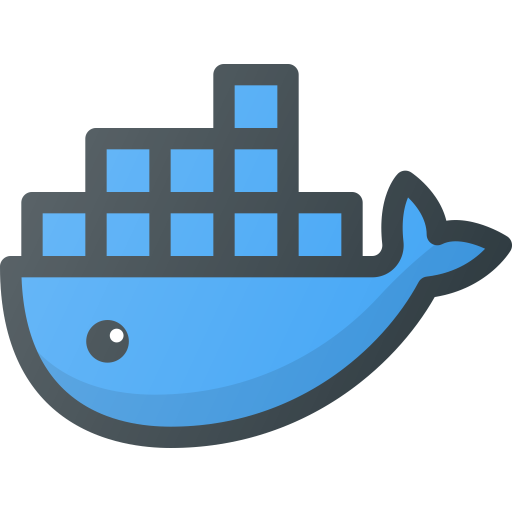
\includegraphics[width=6mm]{../figures/docker_icon.jpg}} ([xshift=-10mm,yshift=-9mm]interior.north west);
    }
}

\newtcblisting{bnflisting}[1][]{%
    #1,
    listing options={
        language=bnf,
        basicstyle=\ttfamily\footnotesize,
        numberstyle=\noncopyable,
        breaklines=true,
        numbers=right,
        showstringspaces=false,
    },
    fonttitle=\ttfamily\small,
    underlay unbroken and first={%
        \path[draw=none] (interior.north west) rectangle node[white]{
\includegraphics[width=5mm]{../figures/bnf_file.png}} ([xshift=-10mm,yshift=-10mm]interior.north west);
    }
}

\newtcblisting{pythonlisting}[1][]{%
    #1,
    listing options={
        language=Python,
        basicstyle=\ttfamily\footnotesize,
        numberstyle=\noncopyable,
        breaklines=true,
        numbers=right,
        showstringspaces=false,
        keywordstyle=\color{blue}\bfseries,
        escapeinside={(*}{*)}
    },
    fonttitle=\ttfamily\small,
    underlay unbroken and first={%
        \path[draw=none] (interior.north west) rectangle node[white]{
\includegraphics[width=5mm]{../figures/python_icon.png}} ([xshift=-10mm,yshift=-10mm]interior.north west);
    }
}

\newtcblisting{rpilisting}[1][]{%
    listing options={
        language=BashPrompt,
        basicstyle=\ttfamily\footnotesize,
        numberstyle=\noncopyable,
        tabsize=2,
        inputencoding=utf8,
        #1
    },
    underlay unbroken and first={%
        \path[draw=none] (interior.north west) rectangle node[white]{
\includegraphics[width=8mm]{../figures/raspi_icon.png}} ([xshift=-10mm,yshift=-10mm]interior.north west);
    }
}

\tcbset{
    enhanced jigsaw,
    breakable,
    listing only,
    boxsep=-1pt,
    top=-1pt,
    bottom=-0.5pt,
    right=-0.5pt,
    overlay first={
        \node[black!50] (S) at (frame.south) {\Large\ding{34}};
        \draw[dashed,black!50] (frame.south west) -- (S) -- (frame.south east);
    },
    overlay middle={
        \node[black!50] (S) at (frame.south) {\Large\ding{34}};
        \draw[dashed,black!50] (frame.south west) -- (S) -- (frame.south east);
        \node[black!50] (S) at (frame.north) {\Large\ding{34}};
        \draw[dashed,black!50] (frame.north west) -- (S) -- (frame.north east);
    },
    overlay last={
        \node[black!50] (S) at (frame.north) {\Large\ding{34}};
        \draw[dashed,black!50] (frame.north west) -- (S) -- (frame.north east);
    },
    before={\par\vspace{10pt}},
    after={\par\vspace{\parskip}\noindent}
}

\newcommand*{\inlineimg}[1]{%
    \raisebox{-.3\baselineskip}{%
        \includegraphics[
            height=\baselineskip,
            width=\baselineskip,
            keepaspectratio,
        ]{#1}%
    }%
}

\definecolor{slightgray}{rgb}{0.90, 0.90, 0.90}

\usepackage{soul}
\makeatletter
\def\SOUL@hlpreamble{%
\setul{}{3.0ex}%
\let\SOUL@stcolor\SOUL@hlcolor%
\SOUL@stpreamble%
}
\makeatother

\newcommand{\inline}[1]{%
    \begingroup%
    \sethlcolor{slightgray}%
    \hl{\ttfamily\footnotesize #1}%
    \endgroup
}

\newcommand{\tinline}[1]{%
    \begingroup%
    \sethlcolor{slightgray}%
    \hl{\ttfamily\tiny #1}%
    \endgroup
}

% Downloads Table
\usepackage{pgfplots}
\usepackage{filecontents}
\usetikzlibrary{pgfplots.dateplot}

%% Packages utiles.
\usepackage{amssymb,subfigure,icomma}
\usepackage[labelfont=bf, width=\linewidth]{caption}

\def\chapterautorefname{Chapter}
\renewcommand{\sectionautorefname}{\S}
\newcommand{\algorithmautorefname}{Algorithm}
\usepackage{hypcap}
\usepackage{bookmark}

\newtheorem{cor}{\corollaryname}[section]
\newtheorem{deff}[cor]{\definitionname}
\newtheorem{ex}[cor]{\examplename}
\newtheorem{lem}[cor]{\lemmaname}
\newtheorem{prop}[cor]{Proposition}
\newtheorem{rem}[cor]{\remarkname}
\newtheorem{theo}[cor]{\theoremname}

\numberwithin{equation}{section}
\numberwithin{table}{chapter}
\numberwithin{figure}{chapter}

\renewcommand{\baselinestretch}{1.5}

%\AtBeginDocument{\hypersetup{pdfborderstyle={/S/S/W 1}}}
\begin{document}

\version{1}

\title{Programming tools for intelligent systems}

\author{Breandan Considine}

\copyrightyear{2019}

\department{D\'epartement d'informatique et de recherche op\'erationnelle}

\president{Marc Feeley}

\directeur{Liam Paull}

\codirecteur{Michalis Famelis}

\membrejury{Eug\`ene Syriani}

\dateacceptation{La date d'acceptation}

%% Voici les disciplines possibles (voir avec votre directeur):
%% \sujet{statistique},
%% \sujet{mathématiques}, \orientation{mathématiques appliquées},
%% \orientation{mathématiques fondamentales}
%% \orientation{mathématiques de l'ingénieur} et
%% \orientation{mathématiques appliquées}

\sujet{Informatique}

%%
%% Fin des variables à définir. La commande \maketitle créera votre
%% page titre.

\pagenumbering{roman}
\maketitle
\maketitle

% Pour générer la deuxième page titre, il faut appeler à nouveau \maketitle
% Cette page est optionnelle et son inclusion est laissé à la discrétion
% de l'étudiant et du directeur de recherche, ou de tout autre instance
% d'autorité.

%%------------------------------------------------- %
%%              pages iv                            %
%%------------------------------------------------- %
\anglais

\chapter*{Abstract}

Programming tools are computer programs which help humans program computers. Tools come in all shapes and forms, from editors and compilers to debuggers and issue trackers. Each of these facilitates a core task in the programming workflow which consumes cognitive resources when performed manually. In this thesis, we share some lessons learned designing four tools that facilitate the development of intelligent software systems, particularly in robotics settings. First, we introduce an integrated development environment (IDE) for programming in the Robot Operating System (ROS), called Hatchery. Second, we describe Kotlin$\nabla$, a language and type system for differentiable programming, an emerging programming paradigm in intelligent systems. Third, we present an automated test suite for differentiable programming, based on adversarial and metamorphic testing. Fourth, we explore a container infrastructure based on Docker, which enables the development of reproducible robotics software for the Duckietown platform. Finally, we offer some concluding remarks about the past, present and future of programming tools for intelligent systems.

\chapter*{Acknowledgements}
\vspace{-60pt} I would like to thank Gimmey, Mom, Uncle Mark, and Dad for their unfailing love and support. \href{http://hannelita.com/}{Hanneli Tavante} for teaching me type theory and the beauty of functional programming. Siyan Wang for his fellowship and adventures. \href{https://laverne.edu/directory/person/xiaoyan-liu/}{Xiaoyan Liu} for planting in me the seed of mathematics. Uncle Andy for watering the seed for many years. Aunt Shannon, Adam Devoe and Jacquie Kirrane for encouraging me to pursue grad school. \href{https://www.cs.rit.edu/~anh/}{Arthur Nunes-Harwitt} for teaching me algorithmic differentiation a long time ago. \href{https://www.sas.rochester.edu/bcs/people/faculty/miller_renee/index.html}{Renee Miller} for sparking my interest in neural science. \href{http://blog.locut.us}{Ian Clarke} for showing me a clever new language called \href{https://kotlinlang.org/}{Kotlin}. \href{https://hadihariri.com/}{Hadi Hariri} for placing more trust in me than I deserved. \href{https://www.jooq.org/}{Lukas Eder} and \href{https://jonnyzzz.com/}{Eugene Petrenko} for showing me the magic of type-safe DSLs and giving me advice about grad school. \href{https://github.com/rusi}{Rusi Hristov} for his patience and mentorship. \href{https://scholar.google.ca/citations?user=PsKlNzUAAAAJ}{Dmitry Serdyuk} for introducing me to Montr\'eal. \href{https://scholar.google.ca/citations?user=-Ss9QGkAAAAJ}{Isabela Albuquerque} and \href{https://scholar.google.ca/citations?user=hkO47vsAAAAJ}{Jo\~ao Monteiro} for showing me what good research looks like. \href{https://takeitallsource.github.io}{Manfred Diaz} and \href{https://pointersgonewild.com/}{Maxime Chevalier Boisvert} for the inspiration, conversations and feedback. \href{https://fgolemo.github.io/}{Florian Golemo} for his excellent engineering and architectural advice. \href{http://TurnerComputing.com}{Ryan Turner}, \href{https://saikrishna-1996.github.io}{Saikrishna Gottipati}, \href{https://maivincent.github.io}{Vincent Mai}, \href{https://krrish94.github.io/}{Krishna Murthy}, \href{https://bhairavmehta95.github.io/}{Bhairav Mehta}, \href{http://www.solomatov.me/}{Konstantin Solomatov} and \href{https://www.seas.upenn.edu/~xsi/}{Xujie Si} for the interesting conversations. \href{https://scholar.google.ca/citations?user=bn4xHHIAAAAJ}{Pascal Lamblin}, \href{http://breuleux.net}{Olivier Breleux} and \href{https://scholar.google.ca/citations?user=XE9SDzgAAAAJ}{Bart van Merri\"enboer} and for lighting the path between ML and PL. \href{http://conal.net/}{Conal Elliott} for teaching me the importance of simplicity and denotational semantics. \href{http://christianperone.com}{Christian Perone} for introducing me to PyTorch, \href{https://research.jetbrains.org/researchers/altavir}{Alexander Nozik}, \href{https://twitter.com/headinthebox}{Erik Meijer}, \href{https://scholar.google.com/citations?user=IcuGXgcAAAAJ}{Kiran Gopinathan}, \href{https://medium.com/@elizarov}{Roman Elizarov} and \href{https://cquic.unm.edu/member/jacob.miller/}{Jacob Miller} for their useful comments and feedback related to Kotlin$\nabla$. \href{https://miltos.allamanis.com/}{Miltos Allamanis} for showing me there is room for SE in ML. \href{https://diro.umontreal.ca/accueil/}{Celine Begin} at the Universit\'e de Montr\'eal for helping a stranger on a cold winter's eve in 2017. \href{https://www.iro.umontreal.ca/~monnier/}{Stefan Monnier} for thoughtfully and thoroughly replying to my rambling emails. \href{https://censi.science/}{Andrea Censi} for his advice and encouragement. Last but not least, I wish to thank my brilliant advisors \href{http://liampaull.ca/}{Liam Paull} for taking a chance on an out-of-distribution sample, providing strong gradients and giving me far more credit than I deserved, and \href{https://michalis.famelis.info/}{Michalis Famelis} for teaching me the value of intuitionistic logic, formal methods, and self-discipline. Thank you!

%%------------------------------------------------- %
%%        page v --- Table de matieres              %
%%------------------------------------------------- %

% Pour un mémoire en anglais, changer pour
% \anglais. Noter qu'il faut une permission
% pour écrire son mémoire en anglais.
% \cleardoublepage termine la page actuel et force TeX
% a poussé les éléments flottant (fig., tables, etc.) sur
% la page (normalement TeX les garde en suspend jusqu'à ce
% qu'il trouve un endroit approprié). Avec l'option <twoside>,
% la commande s'assure que la prochaine page de texte est sur
% le recto, pour l'impression. On l'utilise ici
% pour que TeX sache que la table des matières etc. soit
% sur la page qui suit.
%% TABLE DES MATIÈRES
\cleardoublepage
\pdfbookmark[chapter]{\contentsname}{toc}  % Crée un bouton sur
% la bar de navigation
\tableofcontents
% LISTE DES TABLES
\cleardoublepage
%\phantomsection  % Crée une section invisible (utile pour les hyperliens)
\listoftables
% LISTE DES FIGURES
\cleardoublepage
%\phantomsection
\listoffigures

\NoChapterPageNumber
\cleardoublepage
\pagenumbering{arabic}

\chapter{Introduction}\label{ch:introduction}

\setlength{\epigraphwidth}{0.85\textwidth}
\epigraph{``There is a race between the increasing complexity of the systems we build and our ability to develop intellectual tools for understanding their complexity. If the race is won by our tools, then systems will eventually become easier to use and more reliable. If not, they will continue to become harder to use and less reliable for all but a relatively small set of common tasks. Given how hard thinking is, if those intellectual tools are to succeed, they will have to substitute calculation for thought.''}{\begin{flushright}--Leslie \citet{lamport2002discussion}, \href{https://www.microsoft.com/en-us/research/uploads/prod/2016/12/A-Discussion-With-Leslie-Lamport.pdf}{\textit{A Discussion with Leslie Lamport}}\end{flushright}}

Computational complexity is of such concern in computer science that a great deal of the field is dedicated to understanding it through the lens of function analysis and information theory. In software engineering, researchers are primarily interested in the complexity of building software -- the digital manifestation of algorithms on physical hardware. One kind of software complexity is the cognitive effort required to understand a program.\hspace{-.08em}\footnote{This can be approximated by various metrics like cyclomatic or Halstead complexity.} While today's software is becoming rapidly more intelligent, it shows few signs of becoming more intelligible. Better tools are needed for managing the complexity of building software systems.

\textit{The objective of this thesis is to develop methods that reduce the cognitive effort required to build intelligent systems, using developer tools, programming language abstractions, automated testing, and virtualization technology.}

Broadly speaking, intelligent systems differ from ordinary software systems in that they enable machines to detect patterns, perform tasks, and solve problems which they are not explicitly programmed to solve and which human experts were previously incapable of solving by hard-coding explicit rules. Typically, these systems are able to:\\
%
\begin{enumerate}
    \item learn generalizable rules by processing large amounts of data
    \item tune a large number of free parameters (thousands to billions)
    \item outperform well-trained humans in domain-specific tasks
\end{enumerate}
%
While the idea of intelligent systems has existed for decades, three critical developments made modern intelligent systems ultimately successful. First, computer processing power has become faster, cheaper, and much more readily available. Similarly, the digitalization of new datasets has made vast amounts of information available, and data storage costs have plummeted dramatically. (A \$5 thumb drive today has 200 times more storage capacity than a 2,000 pound, 5 MB, IBM hard drive that leased for \$3,000 per month in 1956.) Most importantly, has been the development of more efficient learning algorithms.

In recent years, computer science and software engineering has made significant strides in building and deploying intelligent systems. Nearly every mobile computer in the world is able to detect objects in images, perform speech-to-text and language translation. These breakthroughs were the direct result of fundamental progress in neural networks and representation learning. Also key to the success of modern intelligent systems was the adoption of collaborative open source practices, pioneered by the software engineering community. Software engineers developed automatic differentiation libraries like Theano~\citep{bergstra2010theano}, Torch~\citep{collobert2002torch} and Caffe~\citep{jia2014caffe}, and built many popular simulators for reinforcement learning. The ease of use and availability of these tools was crucial for democratizing deep learning techniques.

Intelligent systems are widely deployed in virtual settings like data science and cloud services. But even with the tremendous success of machine learning algorithms in fully-observable domains like image recognition and speech processing, intelligent systems have yet to be widely adopted in robotics (at the time of writing this thesis). This dilemma can be partly attributed to various theoretical problems such as domain adaption and transfer learning. Yet with the proven capabilities of modern learning algorithms, exponential increase in processing power, and decades-long effort in building physically-embodied intelligent agents, we should have more progress to show. Why has this goal evaded researchers for so long? One reason, we conjecture, is a lack of programming tools and abstractions for designing, developing, deploying and evaluating intelligent systems. In practice, these activities consume a large amount of cognitive effort without the right set of tools and abstractions.

In this thesis, we explore several tools that facilitate the process of building intelligent systems, and which reduce the cognitive effort required to understand an intelligent program. First, we demonstrate an integrated development environment that assists users writing robotics software (\autoref{ch:hatchery}). Next, we show a type-safe domain-specific language for differentiable programming, an emerging paradigm in deep learning (\autoref{ch:kotlingrad}). To test this application, we use a set of techniques borrowed from property-based testing~\citep{fink1997property} and adversarial learning~\citep{lowd2005adversarial} (\autoref{ch:difftest}). Docker containers~\citep{merkel2014docker} are used to automate the building, testing and deployment of reproducible robotics applications on heterogeneous hardware platforms (\autoref{ch:ducker}). Finally, we offer some concluding remarks and lessons learned for incorporating these programming tools in (\autoref{ch:conclusion}).

% Finally, as a proof of concept for these ideas, we build an intelligent system comprised of a mobile autonomous vehicle and an Android mobile application, using the tools previously described (\autoref{ch:case-study}).

\section{Stages in the software development lifecycle}\label{sec:sldc-stages}

\begin{figure}
    \centering
    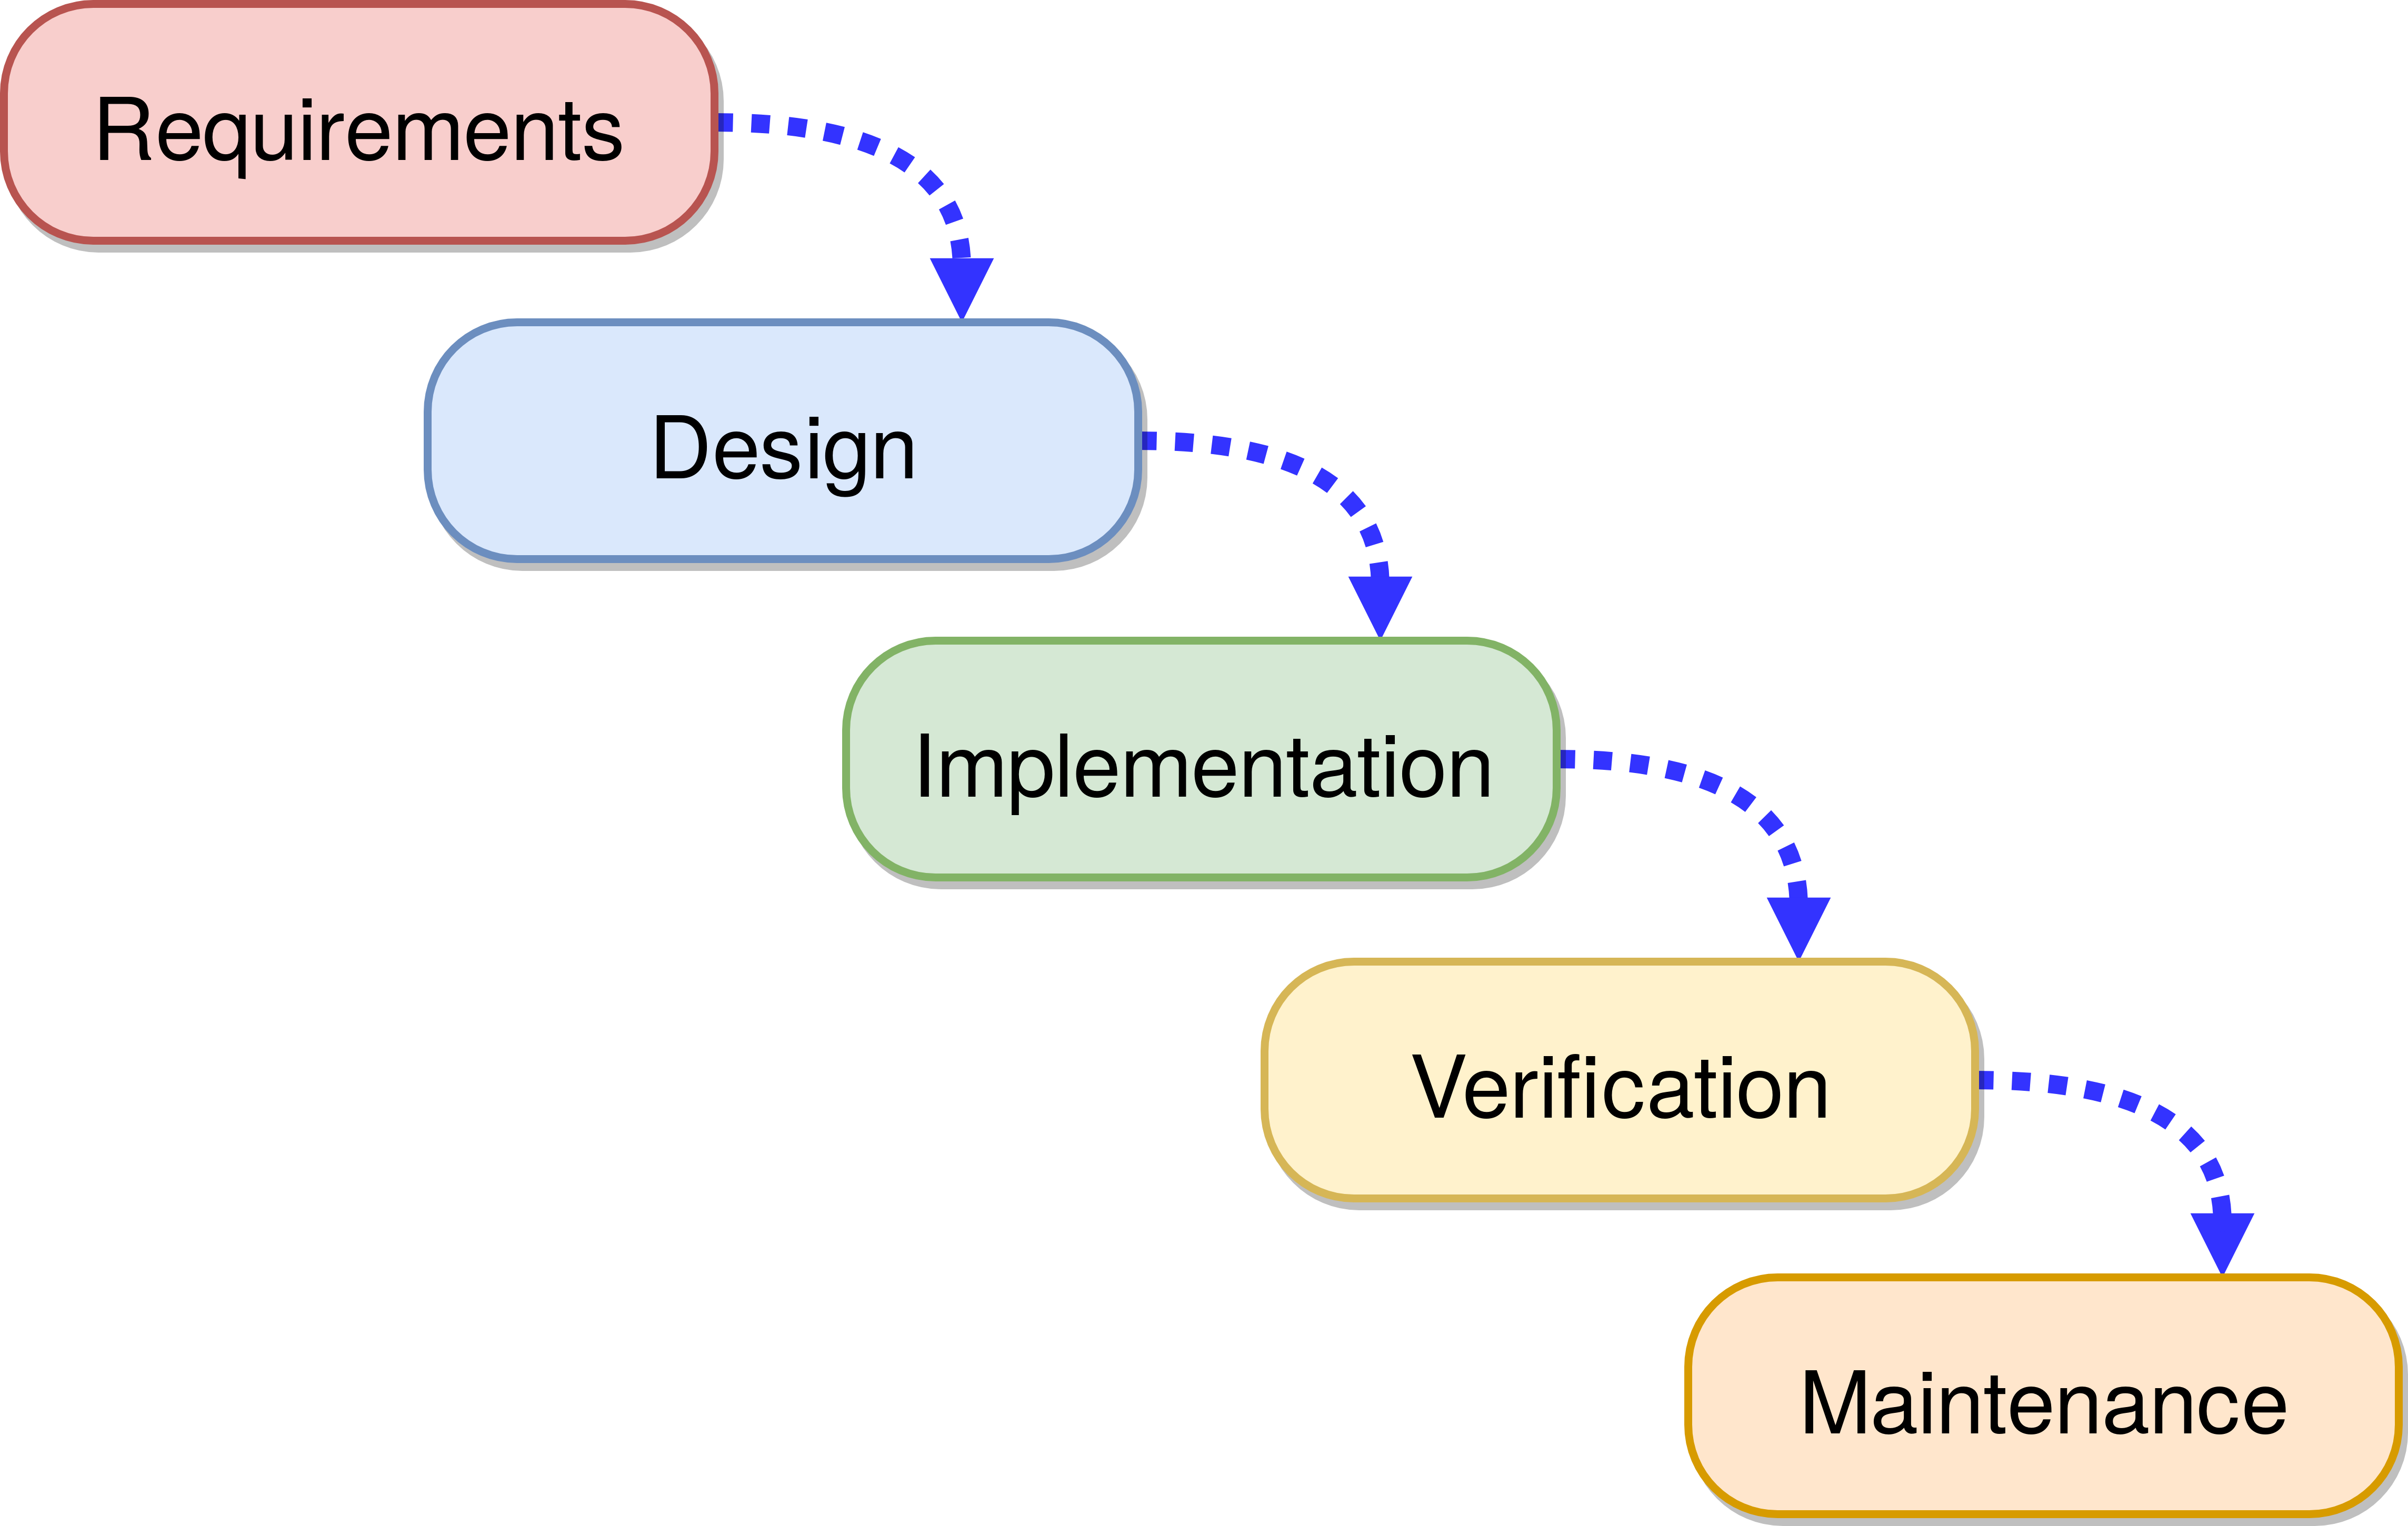
\includegraphics[width=0.70\textwidth]{../figures/waterfall_diagram.png}
    \caption{Royce's original waterfall model describes the software development process. We use it to guide our discussion and frame our contributions inside of this model.\vspace{-10pt}}
    \label{fig:waterfall_model}
\end{figure}

In traditional software engineering, the Waterfall model (\autoref{fig:waterfall_model}) is a classical model for software development comprising of various stages~\citep{royce1987managing}. Intended to describe the traditional software development process, a similar framework can be found in most engineering disciplines. We propose contributions to four stages: \textit{design} in \autoref{ch:hatchery}, \textit{implementation} in \autoref{ch:kotlingrad}, \textit{verification} in \autoref{ch:difftest} and \textit{maintenance} in \autoref{ch:ducker}.

\section{Design: Programming tools for robotics}

Today's software systems are deeply complex entities. Gone are the days where a solitary programmer, even a very skilled one, could maintain a large software system alone. To effectively scale modern software systems, programmers must pool their mental capacity to form a knowledge graph. Software projects which rely on a small set of maintainers tend to perish due to the so-called \textit{bus factor}~\citep{cosentino2015assessing} -- large portions of the knowledge graph are locked inside someone's head. Successful software projects learn how to distribute this graph and form connections to the outside world. The knowledge graph which accumulates around a software project contains facts, but it also contains workflows for programming, debugging, and delivery -- common paths through the labyrinth of software development. Components of this graph can be committed to writing, but documentation is time-consuming and grows stale over time. What is needed is a system that offers the benefits of documentation without the burdens of maintenance.

The development of software systems has a second component, the social graph. The social graph of a successful software project contains product designers, managers and software engineers who work in concert to build software that is well-designed, cohesive, and highly performant. Sometimes this means revising the specification to accommodate engineering challenges, or rewriting source code to remove technical debt. Software design is a multi-objective optimization process and requires contributors with a broad set of skills and common set of goals. To produce software that approximates the criteria of its stakeholders, developers are asked to provide rapid prototypes, and continuously integrate user feedback. Yet today's software systems are larger and more unwieldy than ever. So finding ways to collaborate more effectively is critical to building and maintaining intelligent systems.

First, let us consider the mechanical process of writing software with a keyboard.

Integrated development environments (IDEs) can assist developers building complex software applications by automating certain repetitive programming tasks. For example, IDEs perform static analyses and inspections for catching bugs quickly. They provide completion, refactoring and source code navigation, and they automate the process of building, running and debugging programs. While these tasks may seem trivial, their automation promises increased developer productivity by delivering earlier feedback, detecting clerical errors, and freeing mental resources to be used elsewhere. Rather than being forced to concentrate on the structure and organization of text, if developers are able to manipulate code at a semantic level, they will be much happier and more productive. Furthermore, by automating mechanical tasks in software development, these tools free one's attention towards the fundamental activity of writing and understanding programs.

But what are IDEs really doing? They are guiding developers through the knowledge graph of a software project. Consider what a new developer must learn to get up to speed: in addition to learning the language, developers must learn to use libraries and frameworks (arguably languages in their own right). They must become familiar with command line tools for software development, from build tools to version control and continuous integration. They must become familiar with the software ecosystem, programming styles, conventions and development workflows. And they must learn how to collaborate on a distributed team of developers. By automating common tasks in an interactive programming environment and making the graph connectivity explicit through document markup~\citep{goldfarb1981generalized} and projectional editing~\citep{voelter2014towards}, a well-designed IDE is a tool for graph traversal. It should come as little surprise IDEs are really graph databases.

In some aspects, the development of intelligent systems is no different than classical software engineering. The same principles and best-practices which guide software engineering are also applicable to intelligent systems. And the same activities, from design to maintenance will continue to play an important role in building intelligent systems. But in other respects, the generic programming tools used to develop traditional software will require domain-specific adaptations for learning systems to become truly first-class citizens in the next generation of intelligent software, particularly in the case of robotics development.

Towards that goal, we developed an IDE for the \href{https://www.ros.org/}{Robot Operating System} (ROS) called \href{https://github.com/duckietown/hatchery}{Hatchery}. It supports a number of common workflows for ROS development, such as creating ROS nodes, Gazebo simulator integration, support for remote debugging, static analysis, autocompletion and refactoring. In \autoref{ch:hatchery} we discuss the implementation of these features and some of the challenges of building language support, programming tools and integrating with the ROS middleware. We argue that such tools reduce the cognitive complexity of building ROS applications by adopting explicit coding conventions, annotating unstructured text and automating repetitive development tasks.

\section{Implementation: Type-safe differentiable programming}

In the early days of machine learning, it was widely believed that human-level intelligence would emerge from a sufficiently descriptive first-order logic. By accumulating a database of facts and their relations, researchers believed they could use symbolic reasoning to bypass learning altogether. This rule-based approach dominated a large portion of early research in artificial intelligence and considerable effort was poured into the creation of domain-specific ontologies to capture human knowledge. Despite the best efforts of roboticists, signal processing engineers and natural language researchers, \textit{expert systems} were unable to scale to real-world applications, causing a great disillusionment in artificial intelligence research for several decades. While computer scientists underestimated the difficulty of \text{learning}, expert systems excelled in areas where current machine learning systems struggle such as classical reasoning and interpretability, and there is growing evidence to suggest many of these ideas were simply ahead of their time. In our work, we take inspiration from some early work in symbolic reasoning, type systems and functional programming.

What was finally shown to scale, is the idea of connectionist learning. By nesting random function approximators, called perceptrons, and updating the free parameters using backpropagation~\citep{werbos1990backpropagation, rumelhart1988learning}, the resulting system is capable of learning a surprising amount of intelligent behavior. The approach, termed artificial neural networks (ANNs), can be traced back to the mid-20th century~\citep{ivakhnenko1965cybernetic, rosenblatt1958perceptron}, but was not fully-realized in silico until after the widespread availability of cheap computing and large datasets~\citep{lecun2015deep}. In theory, a single layer of nesting is able to approximate any continuous differentiable function~\citep{hornik1989multilayer}, but in practice, learning requires composing many such approximators in a deeply nested fashion, hence the term, \textit{deep neural networks} (DNNs). The importance of depth was suspected for many years, but the original backpropagation algorithm had difficulty training DNNs due to the vanishing gradient problem~\citep{bengio1994learning}. Solving this problem required a number of adaptations and many years to fully debug. It was not until circa 2013 when deep learning was competitive with human experts in specific domains.

While it took fundamental research in deep learning to realize the connectionist blueprint, the success of modern deep learning can be partly attributed to software tools for calculating mathematical derivatives, a key step in the backpropagation algorithm. Although it has not yet been established if or how derivatives might be calculated in biological circuits, derivatives are essential for ANN training. For many years, the symbolic form of these derivatives were analytically derived when prototyping a new neural network architecture, a tedious and error-prone process. There is a well-known algorithm in the scientific computing community dating back to the 1970s, called \textit{automatic differentiation} (AD)~\citep{linnainmaa1970representation, griewank1989automatic}, which is able to calculate derivatives for arbitrary differentiable functions. But surprisingly, it was not until much later, after the development of Theano~\citep{bergstra2010theano} when AD became widely adopted in the machine learning community. This library alone greatly accelerated the pace of deep learning research and spurred the development of others like TensorFlow~\citep{abadi2016tensorflow} and PyTorch~\citep{paszke2017automatic}.

Engineered intelligent systems must think carefully about languages and abstractions. If developers are required to implement backpropagation by hand, they will have scarce time to think about the high-level characteristics of these systems. Similarly, if programming abstractions are too specific, small variations will require costly reimplementation. This is no different from traditional software engineering -- as engineers, we need to choose the right abstractions for the task at hand. Too low-level and the design is lost in the details -- too abstract and the details are lost completely. With deep learning, the necessity of choosing good abstractions is even more important, as the relationship between source code and runtime behavior is already difficult to debug, due to the complexity of neural networks and array programming. One component of that complexity can be found in the type system.

Most existing AD frameworks for machine learning are written in dynamically-typed languages like Python, Lua and JavaScript, with some early implementations including projects like \href{http://deeplearning.net/software/theano/}{Theano}~\citep{bergstra2010theano}, \href{http://torch.ch/}{Torch}~\citep{collobert2002torch} and \href{https://caffe.berkeleyvision.org/}{Caffe}~\citep{jia2014caffe}. Similar ideas have arisen in statically-typed, functional languages, such as Java (\href{https://github.com/uniker9/JAutoDiff}{JAutoDiff}~\citep{nureki2012jautodiff}, \href{https://deeplearning4j.org/}{DL4J}~\cite{team2016dl4j}), Scala (\href{https://tongfei.me/nexus/}{Nexus}~\citep{chen2017typesafe}), F\# (\href{http://diffsharp.github.io/DiffSharp/}{DiffSharp}~\citep{baydin2015diffsharp}), \href{https://www.tensorflow.org/swift}{Swift}~\citep{lattner2018tensorflow}, Haskell (\href{https://github.com/leopiney/tensor-safe}{TensorSafe}~\citep{pineyro2019structure}) et al., but few of these are able to check the shape of multidimensional arrays in their type system, and those which do are typically implemented in experimental languages with sophisticated type-level programming features. In our work, we demonstrate the viability of shape-checked differentiable programming in a widely-used language. This ensures that programs on matrices, if they compile, are the correct shape and can be numerically evaluated at runtime.

\href{https://github.com/breandan/kotlingrad/}{Kotlin$\nabla$} is an embedded domain-specific language (eDSL) for differentiable programming in a language called \href{https://kotlinlang.org}{Kotlin}, a statically-typed programming language with support for asynchronous programming and multi-platform compilation. In Kotlin$\nabla$ (\autoref{ch:kotlingrad}), we describe an algebraically-grounded implementation of forward-mode automatic differentiation with shape-safe tensor operations. Our approach differs from most existing AD frameworks in that Kotlin$\mathbf{\nabla}$ is the first shape-safe AD library fully compatible with the Java type system, requiring no metaprogramming, reflection or compiler intervention to use.

\section{Verification: Testing intelligent systems}

Most naturally arising phenomena, particularly those related to vision, planning and locomotion are high dimensional creatures. Richard Bellman famously coined this problem as the ``curse of dimensionality''. Our physical universe is populated with problems which are simple to pose, but seemingly impossible to solve inside of it. Claude Shannon, a contemporary of Bellman, calculated the number of unique chess games to exceed $10^{120}$, more than the number of atoms in the universe by approximately forty orders of magnitude~\citep{shannon1950chess}. At the time, it was believed that such problems would be insurmountable without fundamental breakthroughs in algorithms and computing machinery. Indeed, while Bellman or Shannon did not live to see the day, it took only half a century of progress in computer science before solutions to problems with the same order of complexity, first discovered in the Cambrian explosion 541 million years ago, were implemented to a competitive margin in modern computers~\citep{pratt2015cambrian}.

While computer science has made enormous strides in solving the common cases, Bellman's curse of dimensionality still haunts the long tail of machine learning, particularly for distributions that are highly dispersed. Because the dimensionality of many real-world functions that we would like to approximate is intractably large, it is difficult to verify the behavior of a candidate solution in all regimes, especially in settings where failure is rare but catastrophic. According to some studies, humans drivers average 1.09 fatalities per hundred million miles~\citep{kalra2016driving}. A new software build for an autonomous vehicle would need to accumulate 8.8 billion miles of driving in order to approximate the fatality rate of a human operator to within 20\% with a 95\% confidence interval. Deploying such a scheme in the real-world would be logistically, not to mention ethically, problematic.

Realistically speaking, intelligent systems need better ways to practice their skills and probe the effectiveness of a candidate solution within a limited computational budget, without harming humans in the process. The goal of this testing is to highlight errors, but ultimately to provide feedback to the system. In software engineering, the real system under test are the ecosystem of humans and machines which provide each other's means of subsistence. The success of this arrangement depends on an external testing mechanism to enforce a minimum bar of rigor, typically some form of hardware- or human-in-the-loop testing. If the testing mechanism is not somehow opposed to the system under test, an intelligent system can deceive itself, which is neither in the system's nor its users' best interest.

More broadly, type checking (as explored in ~\autoref{ch:kotlingrad}) and testing can be seen as part of a wide spectrum of techniques for software verification and validation. The sooner developers can detect software anomalies, the easier they are to fix and the safer autonomous systems can become. Previous techniques in the software testing literature have called for domain experts to handcraft input-output examples or otherwise constrain the search space, but with advances in adversarial machine learning, automated software validation becomes an increasingly attractive proposition.

Towards that end, in \autoref{ch:difftest} we present preliminary work in adversarial fuzz testing, building on prior literature in adversarial learning, metamorphic and property-based testing. A similar technique is used for testing the numerical correctness of Kotlin$\nabla$'s implementation. We present a simple algorithm for property-based shrinking using projected gradient descent and suggest several future directions for improvement.

\section{Maintenance: Tools for reproducible robotics}

One of the challenges of building intelligent systems and programming in general, is the problem of reproducibility. Software reproducibility has several challenging aspects, including hardware compatibility, operating systems, file systems, build systems, and runtime determinism. While writing programs and feeding them directly into a computer may have once been common practice, today's source code is far too removed from its mechanical realization to be meaningfully executed in isolation. Today's handwritten programs are like schematics for a traffic light -- built inside a factory, and which require a city's-worth of infrastructure, cars, and traffic laws to serve their intended purpose. Like traffic lights, source code does not exist in a vacuum -- built by compilers, interpreted by virtual machines, executed inside an operating system, and which follow a specific communication protocol -- programs are essentially meaningless abstractions outside this context.

As necessary in any good schematic, much of the information required to build a program is divided into layers of abstraction. Most low-level instructions carried out by a computer during the execution of a program were not written nor intended to be read by the programmer and have since been automated and forgotten. In a modern programming language like Java, C\# or Python, the total information required to run a simple program often numbers in the trillions of bits. A portion of that data pertains to the software for building and running programs, including the build system, software dependencies, and development tools. Part of the data pertains to the operating system, firmware, drivers, and embedded software. For most programs, such as those found in a typical GitHub repository,\hspace{-.08em}\footnote{\url{https://help.github.com/en/articles/what-is-my-disk-quota}} a vanishingly small fraction of the information corresponds to the source code itself.

Applied machine learning shares many of the same practical challenges as traditional software development, with source code, release and dependency management. The current process of training a deep learning model can be seen as particularly long compilation step, but it differs significantly in that the source code is a high-level language which does not directly describe the computation being performed, but is a kind of meta-meta-program. The first meta-program describes the connectivity of a large directed graph (i.e.~ a computation graph or probabilistic graphical model), parameterized by weights and biases. The tuning of those parameters is another meta-program, describing the sequence of operations required to approximate a program which we do not have access, save for some input-output examples. Emerging techniques in meta-learning and hyper-parameter optimization (e.g.~differentiable architecture search~\citep{liu2018darts}) add even further meta-programming layers to this stack, by searching over the space of directed graphs themselves.

Hardware manufacturers have developed a variety of specialized accelerators to train and run these programs rapidly. But unlike most programming, deep learning is a much simpler model of computation -- so long as a computer can add and multiply, it has the ability to run a deep neural network. Yet due to the variety of hardware platforms which exist and the software churn associated with them, reproducing deep learning models can be painstakingly difficult on new hardware, even with the same source code and dependencies. Many graph formats, or \textit{intermediate representations} (IRs) in compiler parlance, promise hardware portability but if developers are not careful, their models may not converge during training, or may produce different results on different hardware. Complicating the problem, IRs are produced by competing vendors, selling competing chips with incompatible standards (e.g.~MLIR~\citep{mlir}, ONNX~\citep{bai2019}, nGraph~\citep{cyphers2018intel}, Glow~\citep{rotem2018glow}, TVM~\citep{tvm2018} et al.) While some have tried to leverage existing compilers such as GHC~\citep{elliott2018simple} or DLVM/LLVM~\citep{wei2017dlvm}, there are few signs of broader interoperability at the time of writing this thesis.

At the end of the day, researchers need to reproduce the work of other researchers, but the mental effort of re-implementing basic abstractions can impede scientific progress. Tools which facilitate software reproducibility and incremental development are essential. Fortunately, this is the same problem which has concerned the software industry for many years and produced a variety of version control systems (VCS). But VCS alone is insufficient, since these tools are primarily intended to store text. Text-based representations are temporarily stable, but when dependencies are updated and rebuilt, important details about the original development environment can be misplaced. To reproduce a program in its entirety, a snapshot of all digital information available during execution, and ideally, the physical computer itself is needed. Short of a full snapshot, the minimal set of dependencies and a near physical replica is highly desirable. Any variability in the physical or digital dependency graph can be a source of discrepancies which requires time and energy to later isolate.

In order to mitigate the effects of software variability and assist the development of intelligent systems on heterogeneous platforms, we use a developer tool called \href{https://www.docker.com}{Docker}, part of a loosely-related set of tools for build automation and developer operations which we shall refer to as \textit{container infrastructure}. Docker allows developers to freeze a software application and its host environment, allowing developers (e.g.~using a different environment) to quickly reproduce these applications. Docker itself is a technical solution, but also encompasses a set of best-practices and guidelines which are more methodological in nature. While Docker does not address the incompatibility of vendor standards and hardware drivers, it makes these variables explicit, and reduces the difficulty of reproducing software artifacts.

There is a second component to software reproducibility of intelligent systems, which incorporates the notion of time: simulators. Simulators are used in nearly every engineering discipline to imitate a physical process which may be expensive, dangerous or impractical to bring into reality. For example, simulators are often used to model the dynamics of another instruction set architecture~\citep{bellard2005qemu}, the dynamics of electromagnetic transients~\citep{tavante2018opensi}, the dynamics of orbital motion~\citep{bellman1965wengert}, the dynamics of human transportation systems~\citep{ruch2018amodeus}, or the dynamics of driving~\citep{gym_duckietown}. Today's computers are capable of running increasingly high fidelity simulations, but most practitioners agree that simulation alone will never be enough to capture the full distribution of real-world data. In this view, simulation can be a useful tool for detecting errors, but it cannot fully reproduce all the subtleties of the real-world, and should not be a surrogate for testing on real-world data. Others have suggested a middle road~\citep{bousmalis2018using}, where judicious use of simulator training, alongside domain adaptation is a sufficiently rigorous environment for evaluating intelligent systems. Regardless of which view prevails, our goal is to provide rapid feedback to developers, and to make the entire process from testing to deployment as reproducible as possible.

%\subsection{Case study: An application for autonomous robotics}\label{subsec:case-study}
%
%All great software has a secret recipe: software gets better when its authors use the product. In the best case, the authors are the core users -- ideally by choice, if not by necessity. When software engineers are using their own software on a regular basis -- bumping into sharp corners and encountering edge cases firsthand -- the product gets better. When there is an obviously missing feature, it gets implemented. When there is a bug, it gets fixed. It may not be easy to find users who are so inclined, or to build software which is so useful, but there must be some overlap in order for good software to become great. Termed ``dogfooding''~\citep{harrison2006eating}, this practice is an effective mechanism for building self-improving cybernetic systems and an important principle for open source software and safety-critical systems. Putting this principle into practice, we, as the authors and primary users of these tools, validate their effectiveness by developing a robotics application within an IDE (\autoref{ch:hatchery}), containing Kotlin$\nabla$ code (\autoref{ch:kotlingrad}), tested using adversarial fuzz testing (\autoref{ch:difftest}), and which is built and maintained using the Docker stack (\autoref{ch:ducker}).

\subsection{Iconography}

Throughout this thesis, the following iconography is used to denote: \\
%
\begin{enumerate}
\item[] \inlineimg{../figures/laptop_icon.png} &  Shell commands intended for a personal computer, or output derived thereof. \\
\item[] \inlineimg{../figures/bnf_file.png} & GrammarKit's \inline{.bnf} parsing expression grammar (PEG)~\footnote{GrammarKit usage notes: \url{https://github.com/JetBrains/Grammar-Kit/blob/master/HOWTO.md}} \\
\item[] \inlineimg{../figures/docker_icon.jpg} &  Either \inline{Dockerfile}~\footnote{Dockerfile reference: \url{https://docs.docker.com/engine/reference/builder/}} or Docker Compose~\footnote{Compose file reference: \url{https://docs.docker.com/compose/compose-file/}} syntax. \\
\item[] \inlineimg{../figures/raspi_icon.png}  &  Shell commands which should be run on a Raspberry Pi.\hspace{-.08em}\footnote{Raspberry Pi: \url{https://www.raspberrypi.org/}} \\
\item[] \inlineimg{../figures/duckietown.png}  &  Duckietown Shell (\inline{dts}) commands.\hspace{-.08em}\footnote{Duckietown Shell: \url{https://github.com/duckietown/duckietown-shell-commands}} \\
\item[] \inlineimg{../figures/launch_icon.png}  &  roslaunch \inline{.launch} files.\hspace{-.08em}\footnote{ROS Launch XML: \url{https://wiki.ros.org/roslaunch/XML}} \\
\item[] \inlineimg{../figures/python_icon.png}  &  Python source code.\hspace{-.08em}\footnote{Python documentation: \url{https://www.python.org/doc/}} \\
\item[] \inlineimg{../figures/kotlin_file.png}  &  Kotlin source code.\hspace{-.08em}\footnote{Kotlin documentation: \url{https://kotlinlang.org/docs/reference/}}
\end{enumerate}

\chapter{Programming tools for robotics}\label{ch:hatchery}
\setlength{\epigraphwidth}{0.78\textwidth}
\epigraph{``The hope is that, in not too many years, human brains and computing machines will be coupled together very tightly, and that the resulting partnership will think as no human brain has ever thought and process data in a way not approached by the information-handling machines we know today.''}{\begin{flushright}--Joseph \citet{licklider1960man}, \href{https://groups.csail.mit.edu/medg/people/psz/Licklider.html}{\textit{Man-Computer Symbiosis}}\end{flushright}}

In this chapter we will discuss the design and implementation of an integrated development environment (IDE) for building intelligent robotic software. Modern robots are increasingly driven by systems which learn and improve over time. Most researchers would agree that modern robotic systems have not yet achieved biologically competitive sensorimotor capabilities and most intelligent systems are not physically embodied. However, it is our view that any closed-loop control system that is not explicitly programmed to perform a specific task, but which learns it from experience is an \textit{intelligent system}. Furthermore, any closed-loop system with physical motors is a \textit{robotic system}. While research has demonstrated successful applications in both areas separately, it is widely believed the integration of intelligent systems and robotics will be tremendously fruitful when fully realized.

Hatchery is a tool designed to assist programmers writing robotics applications using the ROS middleware. At the time of its release, \href{https://github.com/duckietown/hatchery}{Hatchery} was the first ROS plugin for the \href{https://www.jetbrains.org/intellij/sdk/docs}{IntelliJ Platform} \footnote{An IDE platform for C/C++, Python and Android development, among other languages.}, and today, is the most widely used with over 10,000 unique downloads. While the idea is simple, its prior absence and subsequent adoption suggest there is unmet demand for such tools in the development of intelligent software systems, particularly in domain-specific applications like robotics.
%

\begin{figure}
\centering
\begin{tikzpicture}
\begin{axis}[
    ybar, ymin=0,
    ylabel=Downloads,
    date coordinates in=x,
    xmin=2017-12-01,
    xmax=2019-06-01,
    xtick=data,
    xticklabel style={
        rotate=70,
        anchor=near xticklabel,
    },
    xticklabel=\year-\month,
    nodes near coords,
    nodes near coords align={vertical},
    height=0.25\textwidth,
    width=0.95\textwidth,
    enlarge x limits=0.03,
    axis x line*=bottom,
    axis y line*=left,
    tick pos=left,
    compat=newest,
]
\addplot table[col sep=comma, x=Category,y=Downloads]{../data/hatchery_downloads.csv};
\end{axis}
\node[above,font=\large\bfseries] at (current bounding box.north) {Unique downloads of Hatchery};
\end{tikzpicture}
\caption{Unique downloads of Hatchery between the time of its release and June 2019. \url{https://plugins.jetbrains.com/plugin/10290-hatchery}.}
\label{fig:hatchery_downloads}
\end{figure}
%
\section{Introduction to the Robot Operating System}

The \href{https://www.ros.org/}{Robot Operating System} (ROS)~\citep{quigley2009ros} is a popular middleware for robotics applications. At its core, ROS provides software infrastructure for distributed messaging, but also includes a set of community-developed libraries and graphical tools for building robotics applications. ROS is not an operating system (OS) in the traditional sense, but it does support similar functionality such as shared memory and inter-process communication. Unlike pure message-oriented systems such as DDS~\citep{pardo2003omg} and \href{https://zeromq.org/}{ZMQ}~\citep{hintjens2013zeromq}, in addition to the communication infrastructure, ROS provides specific APIs for building decentralized robotic systems, particularly those which are capable of mobility. This includes standard libraries for serializing and deserializing geometric data, coordinate frames, maps, sensor messages, and imagery.

The ROS middleware provides several language front-ends for polyglot programming. According to one community census taken in 2018, 55\% of all ROS applications on GitHub are written in C/C++, followed by Python with a 25\%~\citep{Areserio54:online} developer share. Source code for a typical ROS application contains a mixture of C/C++ and Python code, corresponding to the respective language preferences in the robotics and machine learning communities. Hatchery is compatible with most common ROS client libraries, including \href{https://wiki.ros.org/rosjava}{rosjava} for Java, \href{https://wiki.ros.org/rospy}{rospy} for Python, \href{https://wiki.ros.org/rospy}{roscpp} for C/C++, and other language front ends.

\begin{figure}
\centering
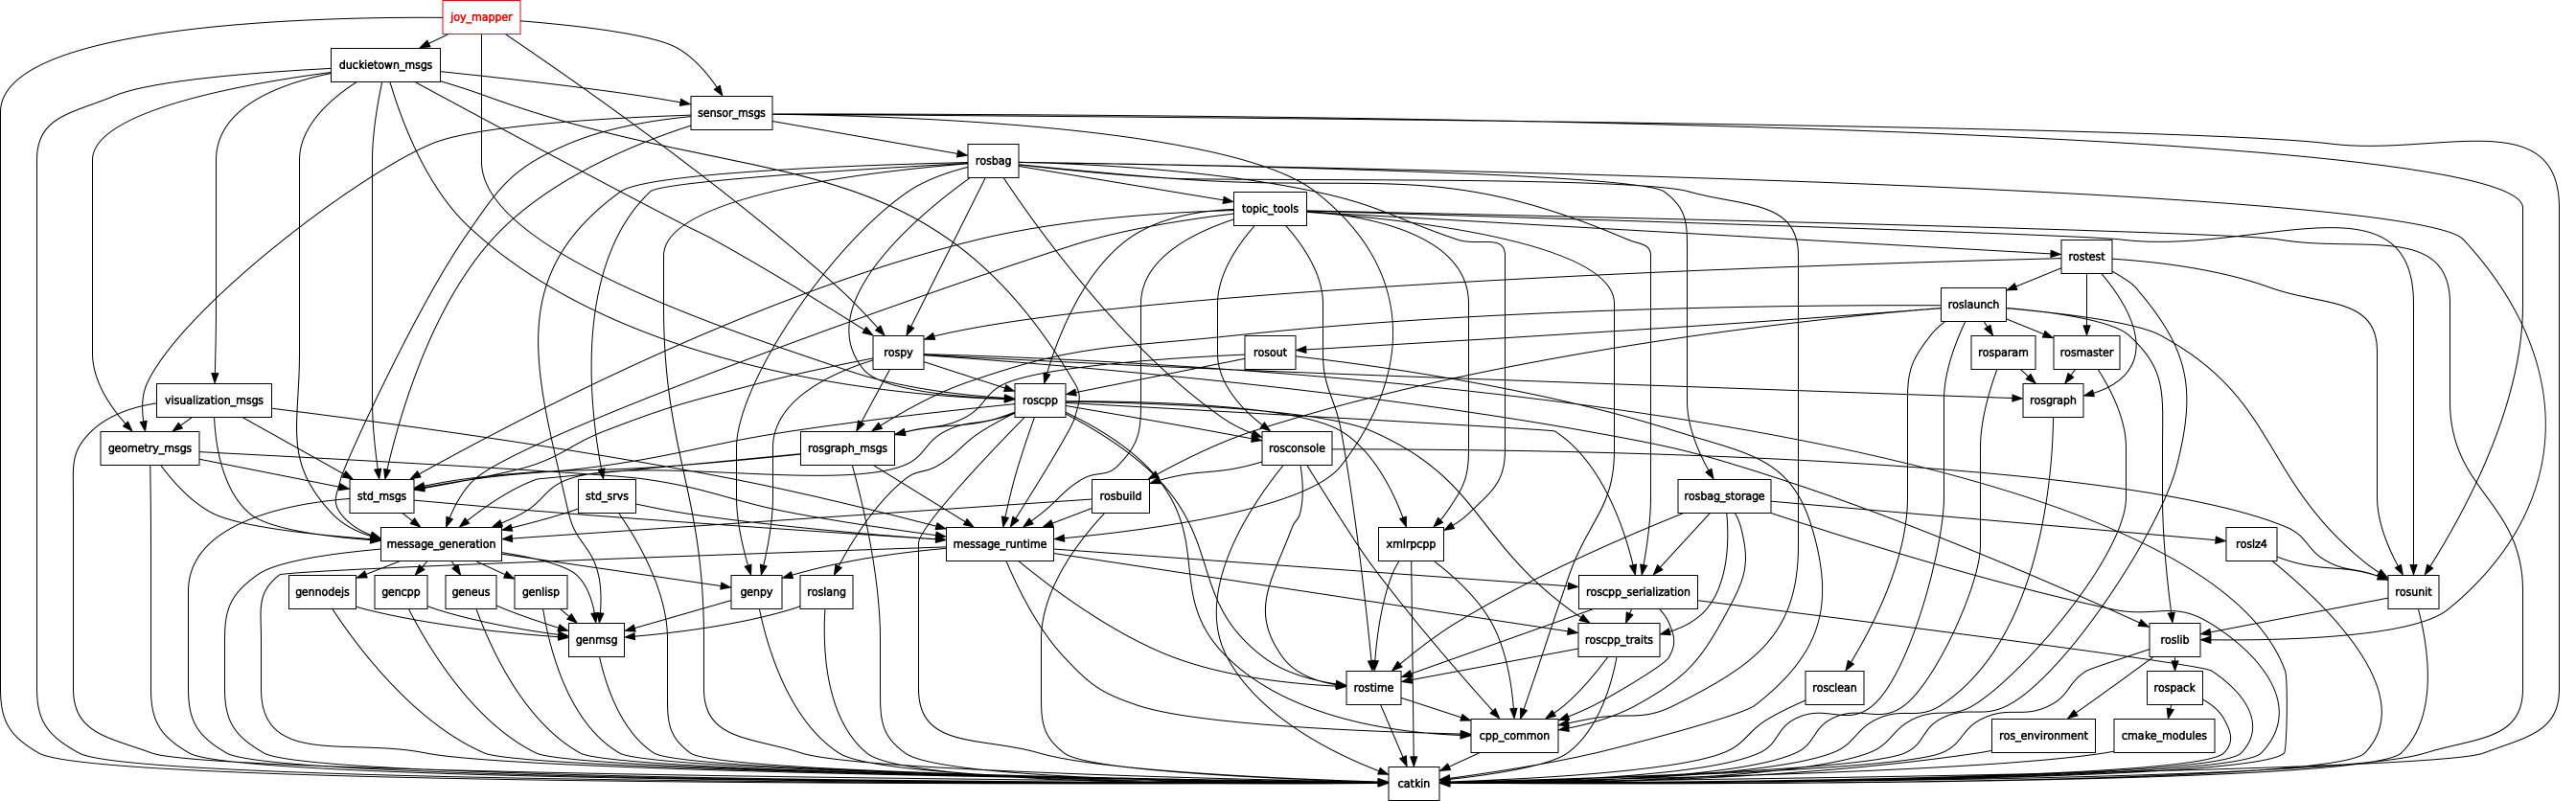
\includegraphics[width=\textwidth]{../figures/rqt_dep_graph.png}
\caption{A typical ROS application contains a large graph of dependencies.}
\end{figure}

A typical ROS project has several components, including the source code, configuration files, build infrastructure, compiled artifacts and the deployment environment. To build a simple ROS application, several steps are necessary. First, one must install the ROS system, which is only officially supported on Debian-based Linux distributions.\hspace{-.08em}\footnote{Detailed installation instructions may be found here: \url{https://wiki.ros.org/ROS/Installation}}
%
Assuming ROS has been installed to the default location, it can be sourced like so:
%
\begin{pclisting}
~$ source /opt/ros/<ROS DISTRO>/setup.[ba]sh
\end{pclisting}
%
A minimal ROS application contains at least one \textit{publisher} and \textit{subscriber}, which pass messages over a shared communication channel. The publisher might be defined as follows:
%
\begin{pythonlisting}[title=./catkin\_ws/src/pubsub/publisher.py]
import rospy
from std_msgs.msg import String

pub = rospy.Publisher("(*\hl{channel}*)", String, queue_size=10)
rospy.init_node("publisher", anonymous=True)
rate = rospy.Rate(10)
while not rospy.is_shutdown():
    pub.publish("Some message")
    rate.sleep()
\end{pythonlisting}
%
As the publisher writes messages to \hl{\ttfamily\small channel}, another node which is subscribed to the same channel will receive a callback when new messages arrive and can read them off the channel:
%
\begin{pythonlisting}[title=./catkin\_ws/src/pubsub/subscriber.py]
def callback(data):
    rospy.loginfo(rospy.get_caller_id() + "received data %s", data.data)

rospy.init_node("subscriber", anonymous=True)
rospy.Subscriber("(*\hl{channel}*)", String, callback)
rospy.spin()
\end{pythonlisting}
%
All ROS packages have launch file, which contain a manifest of available nodes:
%
\begin{launchlisting}[title=./catkin\_ws/src/pubsub/pubsub.launch]
<launch>
<node name="publisher" pkg="pubsub" type="publisher.py" output="screen"/>
<node name="subscriber" pkg="pubsub" type="subscriber.py" output="screen"/>
</launch>
\end{launchlisting}
%
To build and run the application, the following series of commands are required:
%
\begin{pclisting}
~$ cd catkin_ws && catkin_make
\end{pclisting}
%
\begin{pclisting}
~$ roslaunch pubsub pubsub.launch
\end{pclisting}
%
Rather than interacting with the command line, it would be convenient to have a graphical tool to perform all of these tasks automatically. Additionally, it would be helpful to detect if there were a typographical error or navigable reference in the launch file:
%
\begin{launchlisting}[title=./catkin\_ws/src/pubsub/pubsub.launch]
<launch>
<node name="publisher" pkg="pubsub" type="(*\color{red}\textbf{pubsher.py}*)" output="screen"/>
<node name="subscriber" pkg="pubsub" type="(*\color{blue}\underline{subscriber.py}*)" output="screen"/>
</launch>
\end{launchlisting}
%
Notice how the typographical error is printed in red and the valid file reference is underlined in blue, indicating it can be selected to open the file shown above. Broadly, these are the kinds of features IDEs provide and are examples of specific functionality in Hatchery.

\section{Installation}\label{subsec:installation}

\noindent To simply run the tool, users should have the following software dependencies:
%
\begin{enumerate}
    \item MacOS or Debian-based Linux distribution
    \item Robot Operating System (Electric Emys or later)
    \item Java SE (JRE 8+) or CLion/PyCharm 2019.1+
\end{enumerate}
%
\noindent ROS users can use the following command to open an existing ROS project:
%
\begin{pclisting}
~$ git clone https://github.com/duckietown/hatchery && cd hatchery && \
   ./gradlew runIde [-Project="<ABSOLUTE_PATH_TO_ROS_PROJECT>"]
\end{pclisting}
%
\noindent Duckietown users can simply use \inline{dts}, the Duckietown Shell:
%
\begin{dtslisting}
dt> hatchery
\end{dtslisting}
%
\noindent Hatchery can also be installed directly from inside the CLion or PyCharm IDEs, via the following menu options: \menu{File > Settings > Plugins > Marketplace > {\faSearch ``Hatchery''}}

\section{Plugin development}

To build an IDE, some tools are helpful. First, is an IDE, and its source code. Assume that IDE\textsubscript{0} exists. In order to build a new IDE, IDE\textsubscript{1}, we can load the source code from IDE\textsubscript{0} into IDE\textsubscript{0} and use IDE\textsubscript{0}, to modify, compile and re-run the code, which becomes IDE\textsubscript{1}, in which the process is repeated. However, this approach has some disadvantages. First, most IDEs are already quite cumbersome to compile and run. As most auxiliary features are small by comparison, modern IDEs have adopted a modular design, which allows them to load specific packages (i.e.\ \textit{plugins}) as needed. So most developers can skip the first step, and load their plugin inside IDE\textsubscript{0} directly. It is still convenient to have the platform source code for reference purposes, but in most cases this code is read-only.

Hatchery uses the \href{https://www.jetbrains.org/intellij/sdk/docs/}{IntelliJ Platform}, an IDE platform which supports most common programming languages. By targeting a platform with support for polyglot programming, we are able to focus on language-agnostic features in the ROS ecosystem, such as parsing and editing ROS-specific configuration files, build and run configuration and other common development tasks.

\subsection{Refactoring}\label{subsec:refactoring}

Refactoring is an essential feature in any IDE, and the essence of refactoring is renaming. Consider what must occur when a user wishes to rename a token in her program, such as the parameter named \inline{data} on line \#1 below:
%
\begin{pythonlisting}
def callback(data):
    rospy.loginfo(rospy.get_caller_id() + "received data: %s", data.data)
\end{pythonlisting}
%
If she were using the \inline{vim} text editor, one solution would be to replace all textual occurrences of the string \inline{data} within the file using \inline{:\%s/data/msg/g}, producing the following result:
%
\begin{pythonlisting}
def callback((*\hl{msg}*)):
    rospy.loginfo(rospy.get_caller_id() + "received (*\hl{msg}*): %s", (*\hl{msg}*).(*\hl{msg}*))
\end{pythonlisting}
%
There were four occurrences of the string \inline{data}, only two of which were correctly renamed. Instead, only those strings which refer to the function parameter should be renamed:
%
\newcommand{\cfbox}[2]{\colorlet{currentcolor}{.}{\color{#1}\fbox{\color{currentcolor}#2}}}

\begin{pythonlisting}
def callback((*\cfbox{red}{data}*)):
    rospy.loginfo(rospy.get_caller_id() + "received data: %s", (*\cfbox{red}{data}*).data)
\end{pythonlisting}
%
Generally, we would like the ability to rename identifiers across files and languages. To do so, we need a richer understanding of code that transcends text -- we need a parser.

\subsection{Parsing}\label{subsec:the-parser}

One of the most important and unappreciated components of an IDE is the parser. Unlike compilers, most IDEs do not use recursive descent or shift-reduce parsing as treated in most compiler textbooks~\citep{appel2003modern}, as these algorithms are not well-suited for real-time editing of source code. Edits are typically short, localized changes inside a large file, and are frequently invalid or incomplete between keystrokes. As most IDEs are expected to recover from local errors and provide responsive feedback while editing source code, re-parsing the entire program between minor edits would be expensive and unnecessary. In order to analyze source code undergoing simultaneous modification and provide interactive feedback, special consideration must be taken to ensure robust and responsive parsing.

Various techniques have been developed to improve the responsiveness of modern parsers. Incremental parsing techniques like those first proposed in \citet{ghezzi1979incremental} and further developed by \citet{wagner1997practical,wagner1997incremental} seek to incorporate caching and differential parsing to accelerate the analysis of programs under simultaneous modification. Fuzzy parsing techniques like those described in ~\citet{koppler1997systematic} aim to increase the flexibility and robustness of parsing in the presence of local errors. Both of these techniques have played a role in the development of language-aware programming tools, which must be able to provide rapid and specific feedback whilst the user is typing.

The procedural instructions for modern parsers are seldom written by hand unless the language being parsed is very simple or raw performance is desired. Even parsers designed for IDEs, where incremental parsing and error-tolerance is so important, metacompilation toolkits such as ANTLR~\citep{parr1995antlr}, or Xtext~\citep{eysholdt2010xtext} cover a surprising number of common use-cases. Hatchery uses \href{https://github.com/JetBrains/grammar-kit}{Grammar-Kit}, a toolkit designed to assist users developing custom language plugins for the \href{https://www.jetbrains.org/intellij/sdk/docs}{IntelliJ Platform}. It uses a DFA-based lexer generator, JFlex~\citep{klein2001jflex}, and a custom parser-generator loosely based on the parsing expression grammar (PEG)~\citep{ford2004parsing}, a descendant of the Backus-Naur Form (BNF) grammar specification. This specification is consumed by the GrammarKit parser generator and translated to Java source code, producing a parser which reads source code written in the specified language and constructs a program structure interface (PSI), the IntelliJ Platform's internal data structure for representing abstract syntax trees (ASTs). Here is an excerpt of a PEG BNF grammar for parsing ROS \href{https://wiki.ros.org/msg}{\inline{.msg}} files:
%
\begin{bnflisting}
rosInterfaceFile ::= ( property | COMMENT )*
property ::= ( TYPE FIELD SEPARATOR CONSTANT ) | ( TYPE FIELD ) {
    pin=3 // Identifies an unambiguous delimiter or fallback point
    recoverWhile="recover_property" // Error recovery predicate
    mixin="edu.umontreal.hatchery.psi.impl.RosMsgNamedElementImpl"
    implements="edu.umontreal.hatchery.psi.RosMsgNamedElement"
    methods=[getType getKey getValue getName setName getNameIdentifier]
}
private recover_property ::= ! ( TYPE | FIELD | SEPARATOR | COMMENT )
\end{bnflisting}
%
\begin{figure}
\centering
% To regenerate: https://homepage.ruhr-uni-bochum.de/jan.holthuis/posts/using-the-latex-rail-package#manual-compilation-and-latexmk-support
\begin{rail}
( [2] TYPE FIELD ( () | SEPARATOR CONSTANT) ) | ( [1] COMMENT )
\end{rail}
\caption{Railroad diagram for the grammar shown above (reads from left to right).}
\label{fig:railroad}
\end{figure}
%
The lexical rules for the tokens, \inline{TYPE}, \inline{FIELD}, \inline{CONSTANT} et al. are defined in a separate \inline{.flex} file, the \href{https://www.jflex.de/manual.html#Grammar}{JFlex grammar}. Below is an excerpt from the accompanying \inline{.flex} lexer:
%
\begin{flexlisting}
TYPE_CHARACTER=[^:=#\ \r\n\t\f\\]
FIELD_CHARACTER=[^:=#\ \r\n\t\f\\]
SEPARATOR_CHARACTER=[:=]
CONSTANT_CHARACTER=[^\r\n\f#]
COMMENT_CHARACTER=#[^\r\n\f]*
\end{flexlisting}

Grammar-Kit consumes these files and generates Java source code for parsing ROS \href{https://wiki.ros.org/msg}{\inline{.msg}} files. Generated sources can be manually refined to provide support for more advanced functionality such as more flexible error-recovery. For regular languages like the interface description languages (IDL) found in ROS \href{https://wiki.ros.org/msg}{\inline{.msg}} and \href{https://wiki.ros.org/srv}{\inline{.srv}} files, the default generated parser and lexer are usually sufficient. Hatchery is also capable of parsing \href{https://wiki.ros.org/urdf}{URDF}, \href{https://wiki.ros.org/Manifest}{package manifest} and \href{https://wiki.ros.org/roslaunch/XML}{roslaunch} XML.

\subsection{Running and debugging}

The process of compiling and running ROS applications often requires several steps, ex.:
%
\begin{pclisting}
~$ . /opt/ros/<DISTRO>/setup.[ba]sh &&
   cd <PROJECT>/catkin_ws &&
   catkin_make &&
   . devel/setup.sh &&
   [export ROS_MASTER_URI=<URI> &&]
   roslaunch [OPTIONS] src/.../<LAUNCH FILE> [ARGUMENTS]"
\end{pclisting}
%
Hatchery provides assistance for configuring, building and running ROS applications inside a custom graphical user interface (GUI). This GUI effectively serves as a wrapper for the ROS command line interface (CLI). Visual elements like configuration options and command line flags are written to an internal model called the ``Run Configuration'' (\autoref{fig:ros_run_config}). When a run configuration is manually triggered, Hatchery's internal model is serialized to a \inline{String}, representing the command to be executed. This \inline{String} is then sent to a terminal emulator, which invokes the command and displays the corresponding output.

\begin{figure}
\centering
\frame{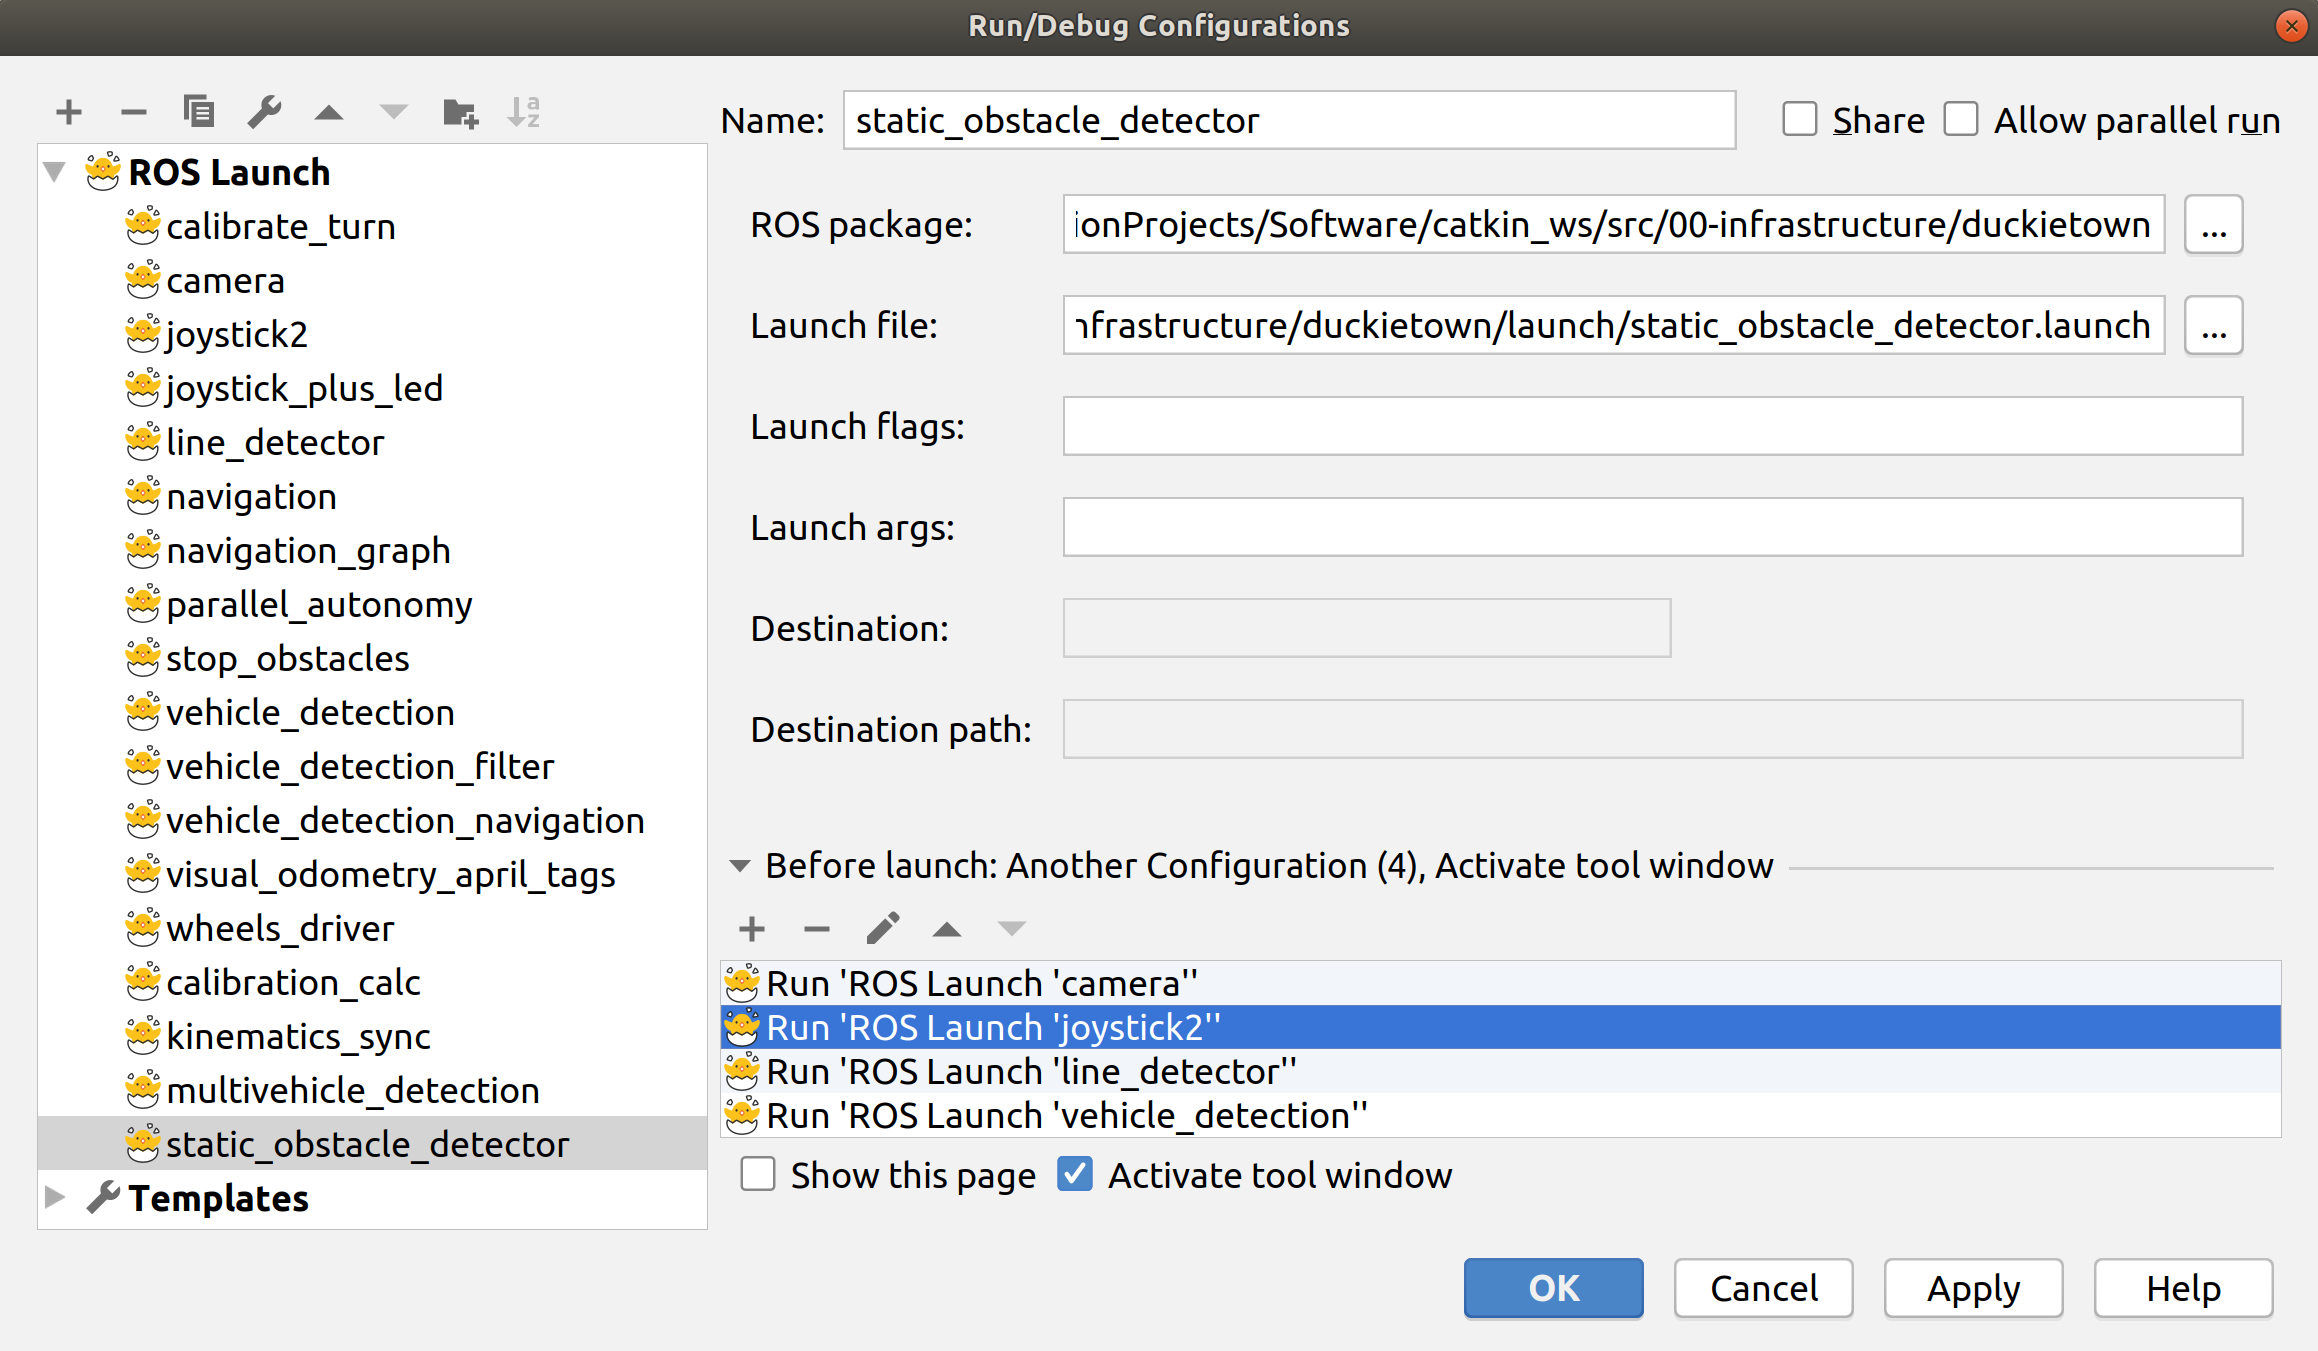
\includegraphics[width=0.90\textwidth]{../figures/ros_run_config.png}}
\caption{ROS Run Configuration. Accessible via: \menu{Run > Edit Configurations > + > ROS Launch}}
\label{fig:ros_run_config}
\end{figure}

\subsection{User interface}

An often overlooked, but important aspect of development tools is the graphical user interface, as the primary interface for editing source code. In the early days of modern computing, the only way of getting information in or out of a computer involved punching holes in paper. Later, computers were equipped with technology to emit the same binary pattern as pixels, which could be used to display a small alphabet called ASCII. With higher density and frequency displays, computers could render more sophisticated shapes and animations. These improvements are the direct result of graphical innovation, but can also be seen as progress in program representation, where the symbolic medium was itself just a notational convention which developers and machines used to communicate.

\begin{figure}
    \centering
    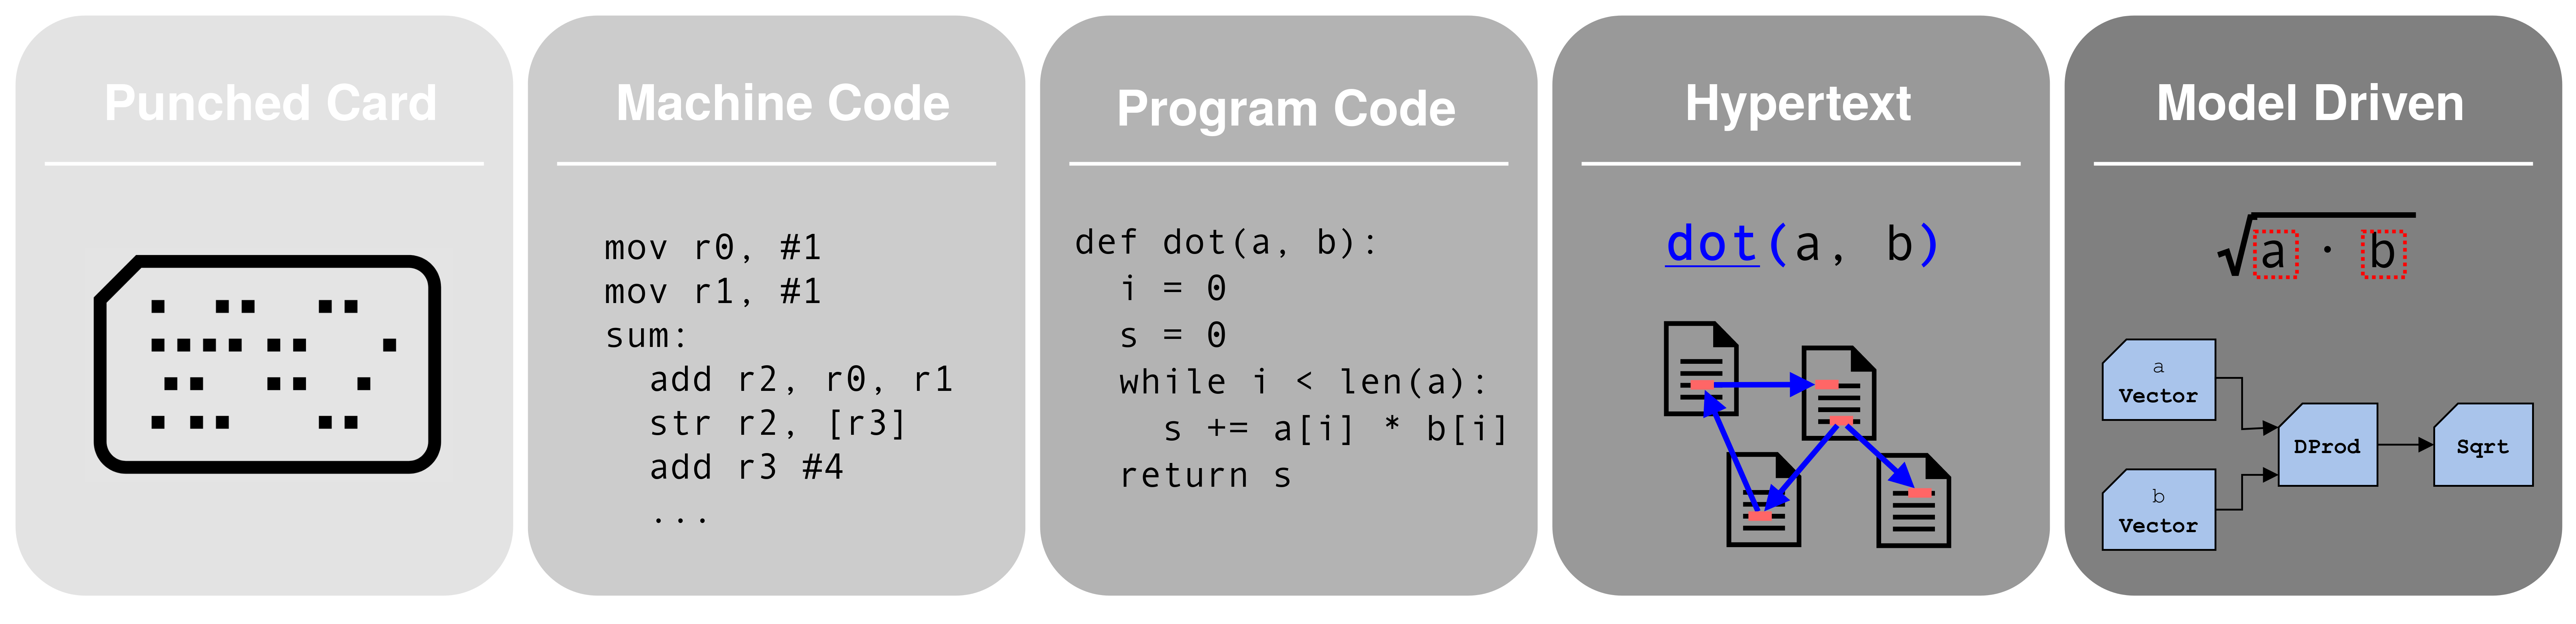
\includegraphics[width=0.90\textwidth]{../figures/progress_in_program.png}
    \caption{The evolution of code. On the left are languages that force the user to adapt to the machine. To the right are increasingly flexible representations of source code.}
    \label{fig:evolution_of_programming}
\end{figure}

ASCII is still the dominant medium for modern programming, although machines still use various forms of low-level assembly code for execution. A great deal of software infrastructure is dedicated to translating between such representations via programming languages and compilers. While many software frameworks provide a minimal command line interface (CLI) and some even provide sophisticated programming environments, these tools are fairly restrictive. In the same way that early computer scientists probably did not invent new algorithms by imagining patterns of holes in paper, ASCII is also an indirect medium for expressing ideas, albeit one slightly less contrived. As hardware and software technology progressed, programming languages moved ``up the stack'', allowing their users to express ideas in a notation which was more familiar and easy to reason about its execution.

\begin{figure}
    \centering
    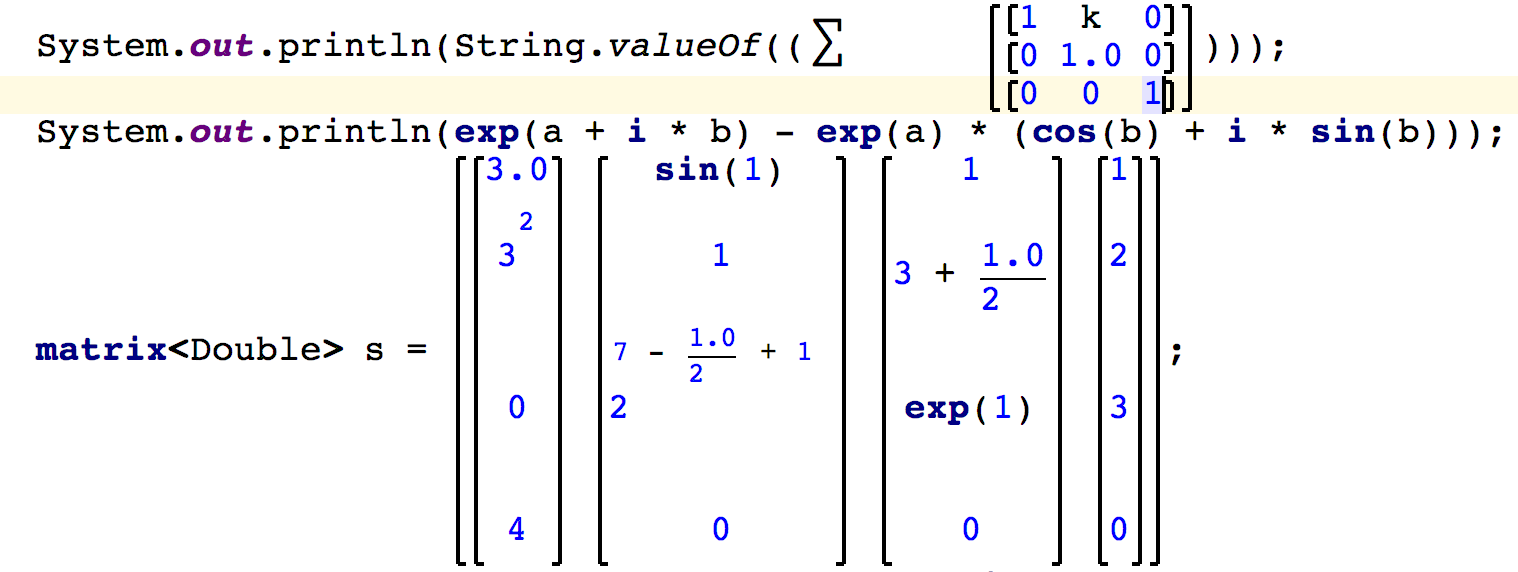
\includegraphics[width=0.90\textwidth]{../figures/mps_screenshot.png}
    \caption{Projectional editors such as \href{https://www.jetbrains.com/mps/}{MPS}~\citep{voelter2010language, pech2013jetbrains} (shown above) are able to render source code in visually creative ways. This might resemble freehand notation or some other visually appealing format.}
    \label{fig:mps_screenshot}
\end{figure}

With the development of modern languages came programming tools capable of representing code as a mixture of hypertext and graphical user interfaces. Such tools provide a richer representation for code than plaintext and help to capture programs' graph-based structure, but still use ASCII with sparse visual cues to render code. Some tools support larger character sets and font-based typographic ligatures, although the visual representation of source code remains mostly linear and textual.

More experimental UIs, as proposed in the language oriented programming~\citep{dmitriev2004language} and model-driven engineering~\citep{famelis2015mummint} literature, suggest the possibility of more visually flexible layouts. This uncoupling between the composition and representation of text raises many intriguing questions. With the proliferation of new abstractions and programming shorthands, what is the appropriate level of notation required for a given programming task? And who is the intended audience? These are important questions to consider when designing a new programming tool.

The Hatchery plugin provides a lightweight GUI overlaying the program's source code. This interface (\autoref{fig:hatchery_gui}) primarily consists of simple visual cues such as text highlighting, navigation assistance and other menus and configuration panels for performing various programming tasks. The host IDE offers a visual language consisting of iconography and repetitive visual motifs, which serve as cognitive landmarks to guide the developer's procedural memory. The IntelliJ Platform offers a palette of common design elements, which users who are familiar with the IDE can recognize at a glance. Plugins can use these same patterns to access procedural memories implanted in the userbase, facilitating transfer learning. To do this properly requires familiarity with the design language and careful integration with the target framework (i.e. ROS).

Hatchery provides a settings menu for configuring and managing ROS installations which can automatically detect local ROS distributions and also allows users to manually configure the \href{https://wiki.ros.org/ROS/Tutorials/InstallingandConfiguringROSEnvironment}{ROS environment}, as shown in ~\autoref{fig:ros_settings}.
%
\begin{figure}[b]
    \centering
    \frame{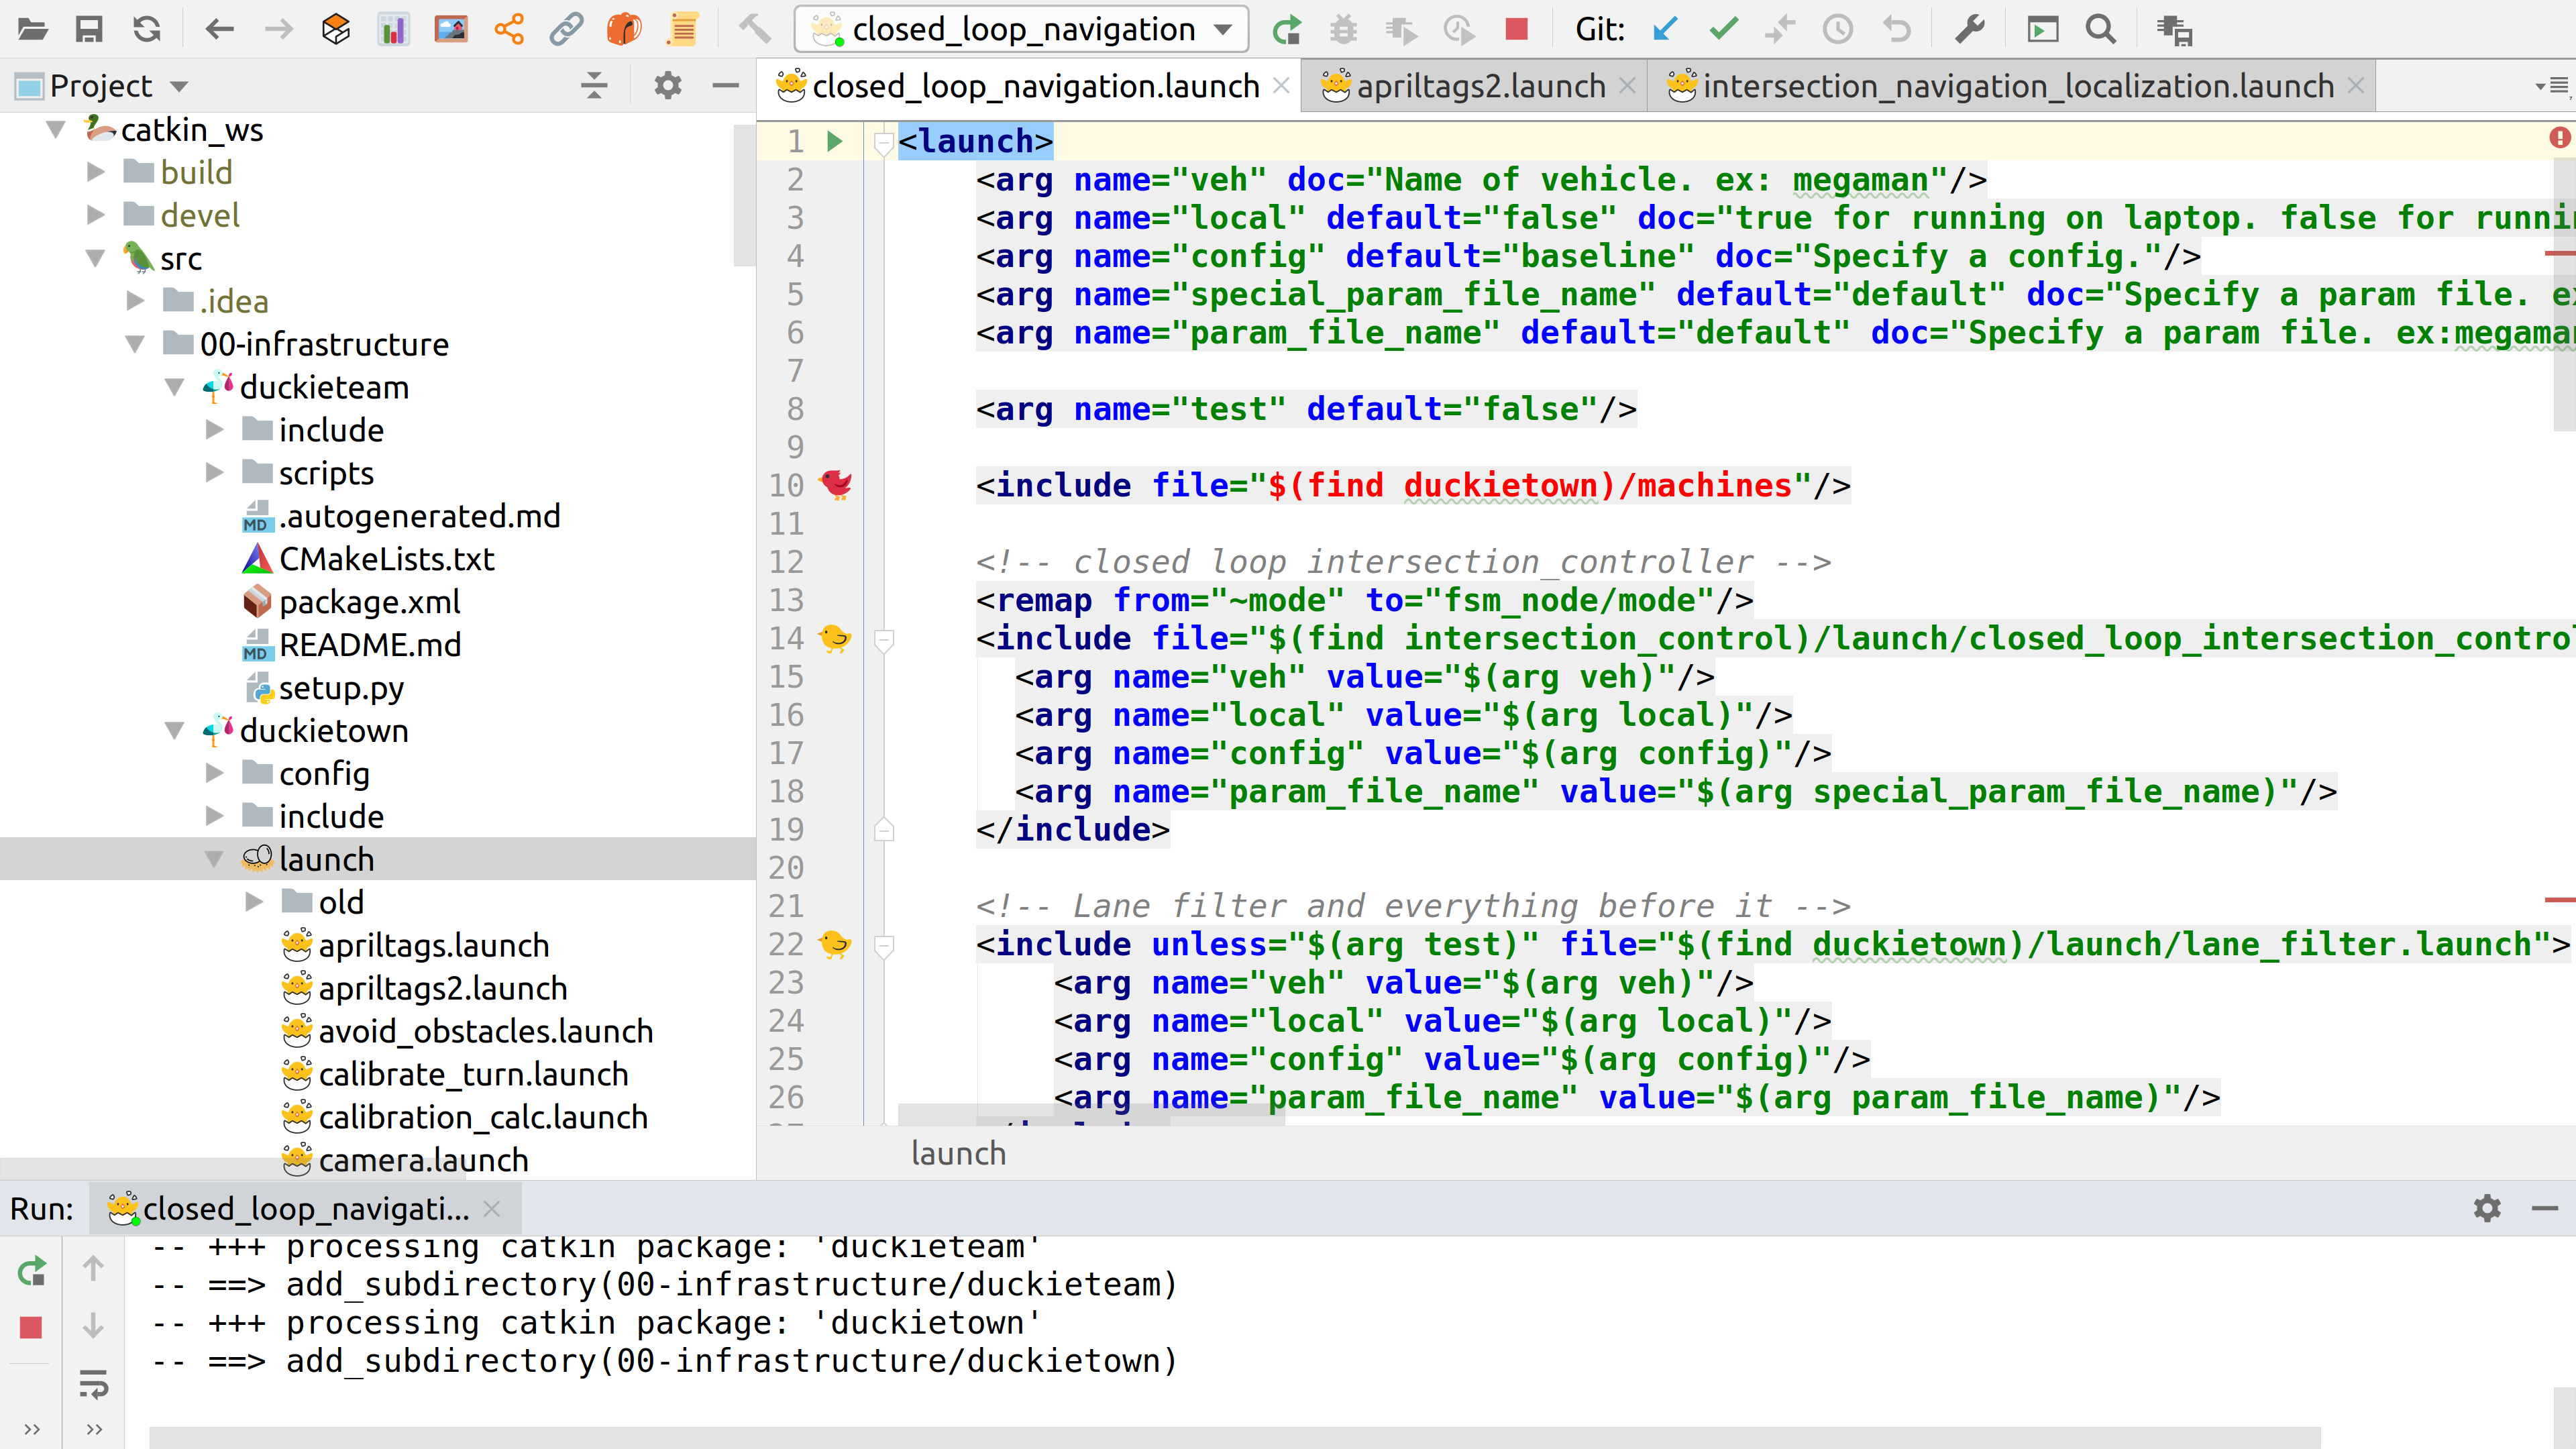
\includegraphics[width=0.90\textwidth]{../figures/hatchery_screenshot.png}}
    \caption{Hatchery UI supports syntax highlighting, validation and project navigation.}
    \label{fig:hatchery_gui}
\end{figure}
%
\begin{figure}
    \centering
    \frame{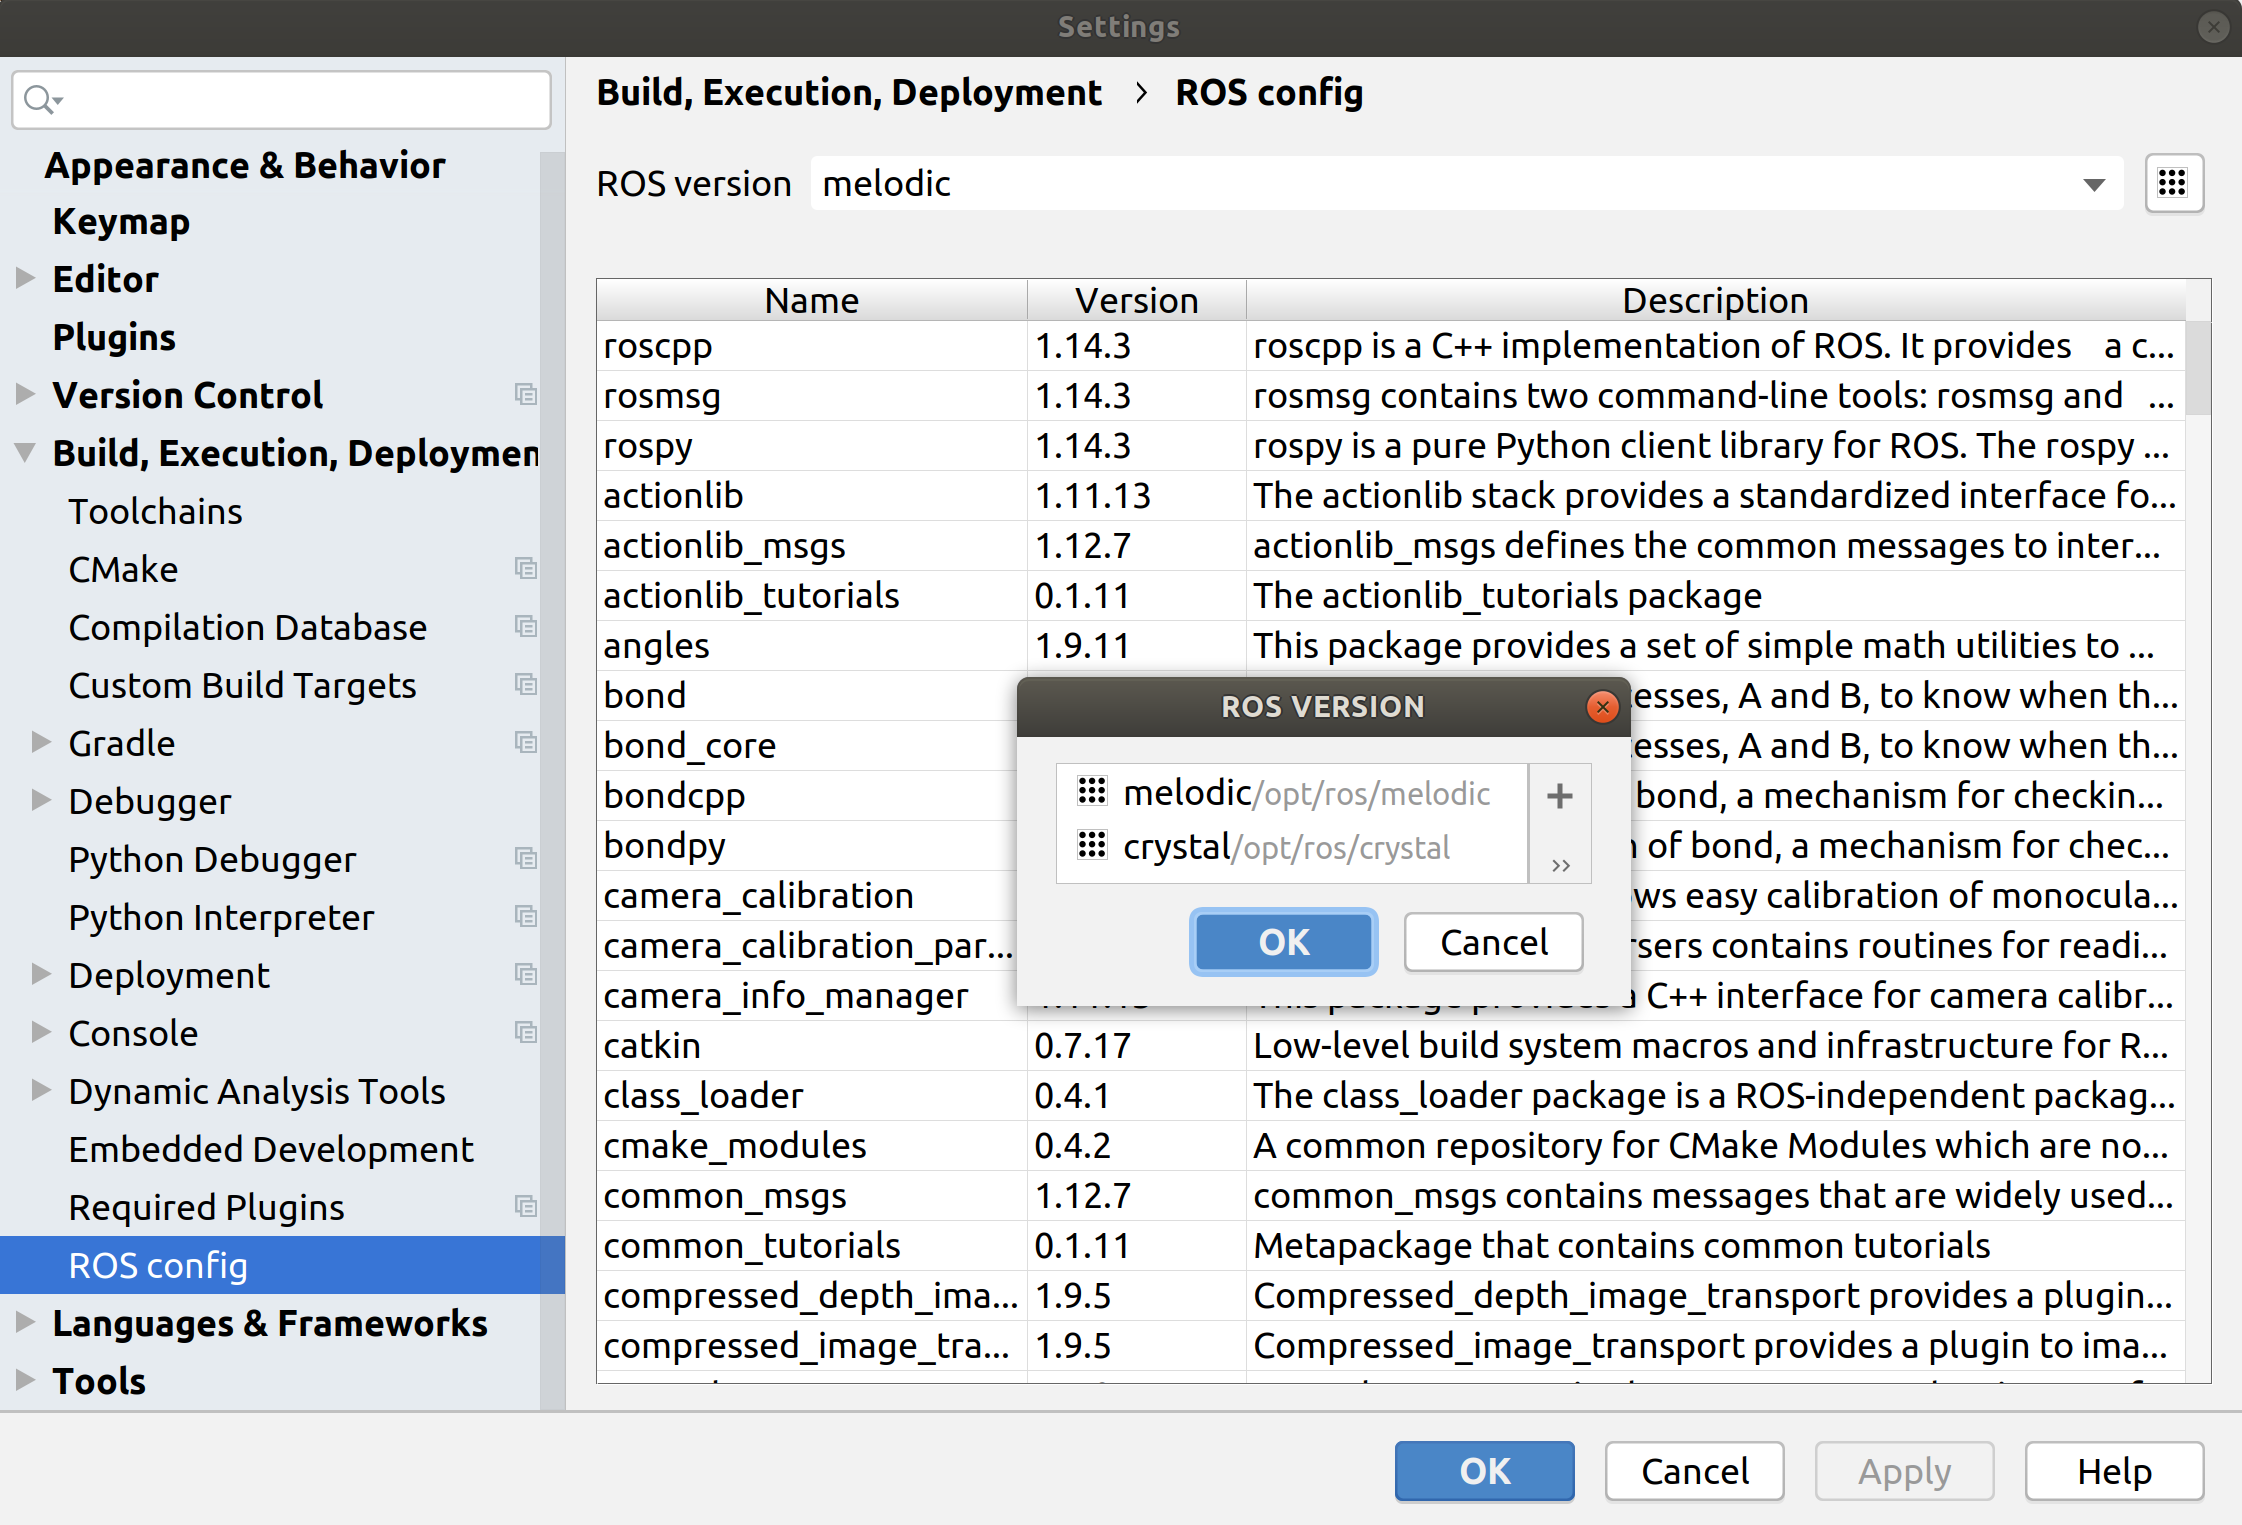
\includegraphics[width=0.90\textwidth]{../figures/ros_settings.png}}
    \caption{Detection of local ROS packages. Accessible via: \menu{File > Settings > ROS config}}
    \label{fig:ros_settings}
\end{figure}

\section{Ongoing work}

\noindent While it supports many common use cases such as rudimentary code navigation, static analysis and run assistance, Hatchery is currently a work in progress. We are working to expand Hatchery's support for ROS programming in some of the following areas:\vspace{10pt}
%
\begin{itemize}
\item \textbf{Syntax support} -- Highlighting, navigation, autocompletion
\item \textbf{Program analysis} -- Code inspections, intentions, and linting
\item \textbf{Testing support} -- Unit and integration testing, code coverage
\item \textbf{Project creation} -- Project setup and boilerplate code generation
\item \textbf{Dependency management} -- Track installed and missing packages
\item \textbf{Monitoring utils} -- Logging, diagnostics, profiling and visualization
\item \textbf{Crash analytics} -- Enhanced stack traces with source navigation
\item \textbf{Build automation} -- Delta rebuilds, cmake magic, code hotswap
\item \textbf{ROS integration} -- Nodes, topics, services, parameters, graphs
\item \textbf{Duckumentation} -- Usage instructions and supported features
\end{itemize}\vspace{10pt}
%
A more comprehensive list of currently supported and upcoming features are detailed below:\vspace{10pt}
%
\begin{multicols}{2}
\begin{todolist}
\item[\done] ROS Launch (\href{https://wiki.ros.org/roslaunch/XML}{\inline{*.launch}}, \href{https://wiki.ros.org/rostest/Writing}{\inline{*.test}})
    \begin{todolist}
    \item[\done] Syntax highlighting
    \item[\done] Resource references (\inline{\$(find <directory>)...})
    \end{todolist}
\item[\done] \href{https://wiki.ros.org/Manifest}{Package manifest (\inline{package.xml})}
    \begin{todolist}
    \item[\done] Syntax highlighting
    \item[\done] \href{https://wiki.ros.org/catkin/package.xml#Dependencies}{Package dependencies} (\inline{<build\_depend>}, \inline{<test\_depend>}, \inline{<run\_depend>})
    \end{todolist}
\item[\done] ROS URDF (\inline{*.urdf.xacro})
    \begin{todolist}
    \item[\done] Syntax highlighting
    \item[\done] Resource references (\inline{\$(find <directory>)...})
    \end{todolist}
\item[\done] \href{https://wiki.ros.org/Bags/Format}{ROS Bag (\inline{*.bag})}
    \begin{todolist}
    \item[\done] Syntax highlighting
    \end{todolist}
\item[\done] \href{https://wiki.ros.org/msg}{ROS Message (\inline{*.msg})}
\item[\done] \href{https://wiki.ros.org/srv}{ROS Service (\inline{*.srv})}
\item[\done] Implement preliminary project structure and XML support
\item[\done] Write an MVP/POC app that supports file renaming and refactoring
\item[\done] Add support for project templates and skeleton project creation
\item[\done] Add support for deploying a project from the local machine to the remote
\item Add support for monitoring and tracking running code, viewing logs
    \begin{todolist}
    \item Live logfile tracking
    \item Save to local disk
    \item Searching the log
    \end{todolist}
\item Collect crash dumps and link to the corresponding code points
    \begin{todolist}
    \item Link stack traces to source code
    \item Copy environment info and crash dump to clipboard
    \end{todolist}
\item Integration with the \href{https://www.ros.org}{Robot Operating System} (ROS)
    \begin{todolist}
    \item[\done] ROS 1 support (\href{https://wiki.ros.org/kinetic}{Kinetic Kame} recommended)
    \item \href{https://github.com/ros2/ros2/wiki}{ROS 2} support
    \item[\done] Managing ROS installations.
    \end{todolist}
\item[\done] \href{http://gazebosim.org/}{Gazebo} simulator integration
\item CMake build integration
\item Remote debugging support
\item Docker integration
    \begin{todolist}
    \item[\done] Basic Docker support
    \item Remote host and script support
    \item \href{https://hub.docker.com}{Docker Hub} namespace awareness
    \item Support for \href{https://platformio.org}{platformio} tooling
    \item X11 forwarding and \href{https://wiki.ros.org/rqt}{rqt} support
    \end{todolist}
\item Static analysis for \href{https://wiki.ros.org/rospy}{Python API} misuse
    \begin{todolist}
    \item[\done] Invalid dependency detection
    \item Validate \inline{.msg}/\inline{.srv} compatibility
    \item ROS nodes and graph analysis via \href{https://wiki.ros.org/rosdep}{\inline{rosdep}}/\href{https://wiki.ros.org/rqt_dep}{\inline{rqt\_dep}}
    \end{todolist}
\item \href{https://wiki.ros.org/rqt}{rqt} plugin support
    \begin{todolist}
    \item[\done] \href{https://wiki.ros.org/rqt_image_view}{\inline{rqt\_img\_view}} - View images
    \item[\done] \href{https://wiki.ros.org/rqt_plot}{\inline{rqt\_plot}} - Plot data visually
    \item[\done] \href{https://wiki.ros.org/rqt_graph}{\inline{rqt\_graph}} - Graph messages
    \item[\done] \href{https://wiki.ros.org/rqt_dep}{\inline{rqt\_dep}} - Visualize dependencies
    \item[\done] \href{https://wiki.ros.org/rqt_bag}{\inline{rqt\_bag}} - Replay and edit bag files
    \item \href{https://wiki.ros.org/rqt_common_plugins}{rqt\_common} - Other common plugins
    \end{todolist}
\end{todolist}
\end{multicols}

\section{Conclusion}

In this chapter we demonstrate the value of IDEs for general purpose software development and present a domain-specific IDE plugin for robotics development, originally developed as a final project in the Duckietown class~\citep{paull2017duckietown}. By using Hatchery, developers can receive assistance when writing, compiling and running ROS applications. The author wishes to express his gratitude to \href{https://github.com/paoloach}{Paolo Achdjian} for contributing several features.

\chapter{Type-safe differentiable programming}\label{ch:kotlingrad}

\setlength{\epigraphwidth}{0.86\textwidth}
\epigraph{``Although mathematical notation undoubtedly possesses parsing rules, they are rather loose, sometimes contradictory, and seldom clearly stated\textellipsis Because of their application to a broad range of topics, their strict grammar, and their strict interpretation, programming languages can provide new insights into mathematical notation.''}{\begin{flushright}--Kenneth \citet{iverson1999math}, \href{https://www.cs.trinity.edu/About/The_Courses/cs301/math-for-the-layman/}{\textit{Math for the Layman}}\end{flushright}}

In this chapter, we will discuss the theory and implementation of a type-safe domain-specific language for automatic differentiation (AD), an algorithm with a variety of applications in numerical optimization and machine learning. The key idea behind AD is fairly simple. A small set of primitive mathematical operations form the basis for all modern computers, and by composing these operations over the real numbers in an orderly fashion, one can compute any computable function. In machine learning, we are often given a computable function in the form of a program which does not work properly. We would like an algorithm for determining how to change the input slightly, to produce a more suitable output.

In 1964, such an algorithm was first conceived in~\citet{wengert1964simple}, whose method is known today as forward-mode AD. Not long after, a certain Richard Bellman reproduced Wengert's algorithm to numerically estimate the orbital dynamics of a two-body system, recognizing its potential for, ``the treatment of large systems of differential equations which might not otherwise be undertaken''~\citep{bellman1965wengert}. Around the same time, key details of the backpropagation algorithm first emerged~\citep{dreyfus1990artificial}. It was in~\citet{linnainmaa1970representation} where the idea of calculating derivatives over computation graphs was first recorded. Linnaimaa's algorithm was particularly important for neural networks, and is today known as reverse-mode AD. But it was not until 2010 when standard software tools~\citep{bergstra2010theano} for AD became widely available in machine learning. It is here where our journey begins.

\section{Automatic differentiation}\label{sec:automatic-differentiation}

Given some input to a function, AD tells us how to change the input by a minimal amount, in order to maximally change the outputs. Suppose we are handed a function $P_k: \mathbb{R}\rightarrow\mathbb{R}$, composed of a series of nested functions, each with the same type:
%
\begin{equation}
    P_k(x) = \begin{cases} p_1 \circ x = x &\text{if } k=1\\ p_k\circ P_{k-1} \circ x&\text{if } k > 1 \end{cases}
\end{equation}
%
From the chain rule, we recall the derivative of a composition is a product of the derivatives:
%
\begin{equation} \label{eq:sfun_chain_rule}
    \frac{dP}{dp_1} = \frac{dp_k}{dp_{k-1}}\frac{dp_{k-1}}{dp_{k-2}}\dots\frac{dp_2}{dp_1}= {\displaystyle \prod_{i=1}^{k-1} \frac{dp_{i+1}}{dp_{i}}}
\end{equation}
%
Given $Q(q_1, \dots, q_m): \mathbb{R}^m\rightarrow\mathbb{R}$, the \textit{gradient} is a function $\nabla Q: \mathbb{R}^m\rightarrow\mathbb{R}\rightarrow\mathbb{R}^m$ defined as:
%
\begin{equation}
    \nabla Q = \left[ \frac{\partial Q}{\partial q_1}, \dots, \frac{\partial Q}{\partial q_m}\right]
\end{equation}
%
The \textit{Hessian} is a function $\mathbf{H}:\mathbb{R}^m\rightarrow\mathbb{R}\rightarrow\mathbb{R}^{m\times m}$ returning a matrix of second-order partials:
%
\begin{equation}
\mathbf{H}(Q) = \begin{bmatrix}{\dfrac {\partial ^{2}Q}{\partial x_{1}^{2}}}&{\dfrac {\partial ^{2}Q}{\partial x_{1}\,\partial x_{2}}}&\cdots &{\dfrac {\partial ^{2}Q}{\partial x_{1}\,\partial x_{m}}}\\[2.2ex]{\dfrac {\partial ^{2}Q}{\partial x_{2}\,\partial x_{1}}}&{\dfrac {\partial ^{2}Q}{\partial x_{2}^{2}}}&\cdots &{\dfrac {\partial ^{2}Q}{\partial x_{2}\,\partial x_{m}}}\\[2.2ex]\vdots &\vdots &\ddots &\vdots \\[2.2ex]{\dfrac {\partial ^{2}Q}{\partial x_{m}\,\partial x_{1}}}&{\dfrac {\partial ^{2}Q}{\partial x_{m}\,\partial x_{2}}}&\cdots &{\dfrac {\partial ^{2}Q}{\partial x_{m}^{2}}}\end{bmatrix}
\end{equation}
%
For vector functions $\mathbf{f}: \mathbb{R}^m\rightarrow\mathbb{R}^n$, the \textit{Jacobian}, $\mathcal{J}_{\mathbf{f}}: \mathbb{R}^m\rightarrow\mathbb{R}^n\rightarrow\mathbb{R}^{n \times m}$ is defined as:
%
\begin{equation}
\mathcal{J}_{\mathbf{f}} =
\begin{bmatrix}
    \dfrac{\partial \mathbf{f}}{\partial x_1} & \cdots & \dfrac{\partial \mathbf{f}}{\partial x_m}
\end{bmatrix} =
\begin{bmatrix}
    \dfrac{\partial f_1}{\partial x_1} & \cdots & \dfrac{\partial f_1}{\partial x_m}\\
    \vdots & \ddots & \vdots\\
    \dfrac{\partial f_n}{\partial x_1} & \cdots & \dfrac{\partial f_n}{\partial x_m}
\end{bmatrix} =
\begin{bmatrix}
    \nabla f_1 \\
    \vdots \\
    \nabla f_m
\end{bmatrix}
\end{equation}
%
For scalar functions, the transpose of the Hessian is equivalent to the Jacobian of the gradient:
%
\begin{equation}
\mathbf{H}(Q)^\intercal = \mathcal{J}_\mathbf{q}(\nabla Q)
\end{equation}
%
For a vector function $\mathbf{P}_k(\mathbf{x}): \mathbb{R}^m\rightarrow\mathbb{R}^n$, the chain rule from \autoref{eq:sfun_chain_rule} still applies:
%
\begin{equation} \label{eq:vfun_chain_rule}
\mathcal{J}_\mathbf{P_k} = \displaystyle \prod_{i=1}^{k} \mathcal{J}_{p_i} = \underbrace{\bigg(\Big((\mathcal{J}_{p_k} \mathcal{J}_{p_{k-1}}) \dots \mathcal{J}_{p_2}\Big) \mathcal{J}_{p_1}\bigg)}_{\textit{``Reverse accumulation''}} = \underbrace{\bigg(\mathcal{J}_{p_k} \Big(\mathcal{J}_{p_{k-1}} \dots (\mathcal{J}_{p_2} \mathcal{J}_{p_1})\Big)\bigg)}_{\textit{``Forward accumulation''}}
\end{equation}
%
For completeness, but rarely used in practice, is the second-order partials for vector functions:
%
\begin{equation}
\mathbf{H} (\mathbf {f} )=[\mathbf {H} (f_{1}), \mathbf {H} (f_{2}), \dots, \mathbf {H} (f_{n})]
\end{equation}
%
We can use these tools to compute the direction to adjust the inputs of a computable function, in order to maximally change that function's output, i.e.\ the direction of steepest descent.

\noindent Sometimes a function has the property that given an input $a$, no matter how $a$ is changed, the output remains the same. We say that such functions have zero gradient for that input.
%
\begin{equation}
    (\nabla F)(a) \approx \mathbf{0}
\end{equation}
%
The cost of calculating the Hessian, $\mathbf{H}$ is approximately quadratic~\citep{griewank1993some} with respect to the number of independent variables under differentiation. If $\mathbf{H}(a)$ is tractable to compute and invertible, we could use the second-partial derivative test to determine that:\\
%
\begin{enumerate}
    \item If all eigenvalues of $\mathbf{H}(a)$ are positive, $a$ is a local minimum
    \item If all eigenvalues of $\mathbf{H}(a)$ are negative, $a$ is a local maximum
    \item If $\mathbf{H}$ contains a mixture of positive and negative eigenvalues, $a$ is a \textit{saddle point}\\
\end{enumerate}
%
For some classes of computable functions, small changes to the input will produce a sudden large change in the output. We say that such functions are non-differentiable.
%
\begin{equation}
    ||\nabla F|| \approx \pm \infty
\end{equation}
%
It is an open question whether non-differentiable functions exist in the real-world~\citep{buniy2005hilbert}. At the current physical (10nm) and temporal (10ns) scale of modern computing, there exist no such functions, but most modern computers are incapable of reporting the true value of their binary-valued functions. For all intents and purposes, programs implemented by most physical computers are discrete relations. Nevertheless, discrete programs are capable of approximating bounded functions on $\mathbb{R}^m$ to arbitrary precision given enough time and space. For most applications, a low precision (32-64 bit) approximation is sufficient.

There exists at the heart of machine learning a theorem that states a simple family of functions, which compute a weighted sum of a non-linear function $\varphi: \mathbb{R} \rightarrow \mathbb{R}$ composed with a linear function $\theta^\intercal x + b$, can approximate any bounded function on $\mathbb{R}^m$ to arbitrary precision. More precisely, the universal approximation theorem~\citep{hornik1989multilayer} states that for all real-valued continuous functions $\mathbf{f}: C(\mathbb{I}_m)$, where $\mathbb{I}_m = [0, 1]^m \rightarrow [0, 1]$, there exists a function $\mathbf{\hat f}: \mathbb{R}^m \times \mathbb{R}^{n \times m}$, parameterized by $\Theta \in \mathbb{R}^{n \times m}$, taking an input $\mathbf x \in [0, 1]^m$ and constants $n \in \mathbb{N}, \mathbf{\beta} \in \mathbb{R}^n, \mathbf{b} \in \mathbb{R}^n, \epsilon \in \mathbb{R}^+$ such that following statement holds:
%
\begin{equation}
    \begin{split}
        \mathbf{\hat{f}}(\mathbf{x}; \Theta) = \mathbf{\beta}^\intercal \varphi_{\odot} \left(\Theta^\intercal \mathbf{x} + \mathbf{b}\right) \\
        \forall \mathbf{x} \in \mathbb{I}_m, \ | \mathbf{\hat f}( \mathbf{x} ) - \mathbf{f} ( \mathbf{x} ) | < \epsilon
    \end{split}
\end{equation}
%
Where $\varphi_{\odot}$ indicates the nonlinear function $\varphi$ applied elementwise to a vector. This theorem only tells us that $\Theta$ exists, but does not tell us how to find it nor does it place an upper bound on the constant $n$, somewhat limiting its practical applicability. But for reasons not yet fully understood, empirical results suggest it is possible to approximate many naturally-arising functions in a relatively short number of steps by composing several \textit{layers} of $\Theta^\intercal \mathbf{x} + \mathbf{b}$ and $\varphi$ in an alternating fashion, and updating each $\Theta$ using a procedure based on gradient descent. The resulting model might be expressed as follows\footnote{The notation below assumes some familiarity with currying and partial function application, in which $\mathbf{\hat P}: \mathbb{R}^m \rightarrow \mathbb{R}^n \equiv \underbrace{\mathbb R \rightarrow \ldots \rightarrow \mathbb R}_{m}\rightarrow \mathbb{R}^n$. For further details, see \citet{schonfinkel1924bausteine, curry1958combinatory} et al.},
%
\begin{equation} \label{eq:recursive_parametric_eq}
    \mathbf{\hat P}_k(\mathbf{x}; \bm\Theta) = \begin{cases} \mathbf{\hat p}_1(\Theta_1)\circ\mathbf{x} &\text{if } k=1\\ \mathbf{\hat p}_k(\Theta_k)\circ \mathbf{\hat P}_{k-1}(\bm\Theta_{[1, k-1]})\circ\mathbf{x}&\text{if } k > 1 \end{cases} \\
\end{equation}
%
where $\bm\Theta = \{\Theta_1, \dots, \Theta_k\}$ are free parameters and $\mathbf{x} \in \mathbb{R}^m$ is a single input. To approximate $\mathbf{P}(\mathbf x)$, one must obtain $\mathbf{X} = \{\mathbf{x}^{(0)}, \dots, \mathbf{x}^{(z)}\}, \mathbf{Y} = \{\mathbf{y}^{(0)} = \mathbf{P}(\mathbf{x}^{(0)}), \dots, \mathbf{y}^{(z)} = \mathbf{P}(\mathbf{x}^{(z)})\}$ in as great and varied a quantity as possible and repeat the following procedure until $\bm\Theta$ converges:
%
\begin{equation} \label{eq:stochastic_grad_descent}
    \bm\Theta \leftarrow \bm\Theta - \alpha\frac{1}{z}\nabla_{\bm\Theta} \sum_{i=1}^z\mathcal{L}\big(\mathbf{\hat P}_k(\mathbf{x}^{(i)}; \bm\Theta), \mathbf{y}^{(i)}\big)
\end{equation}
%
In the general case, we can solve for the gradient using \autoref{eq:vfun_chain_rule}. For most common $\mathcal{L}$, the complexity of this procedure is linear with $z$. As $z$ can be quite large in practice, and since obtaining the exact gradient is not important, we use a stochastic variant by resampling a \textit{minibatch} $\mathbf{X}', \mathbf{Y}'$ consisting of pairs $\mathbf{x}^{(i)}, \mathbf{y}^{(i)}$ for $i \sim \{0, ..., z\}$ without replacement on each update step. This is slightly noisier, but runs considerably more quickly.

\section{Differentiable programming}\label{sec:differentiable-programming}

\begin{figure}
    \centering
    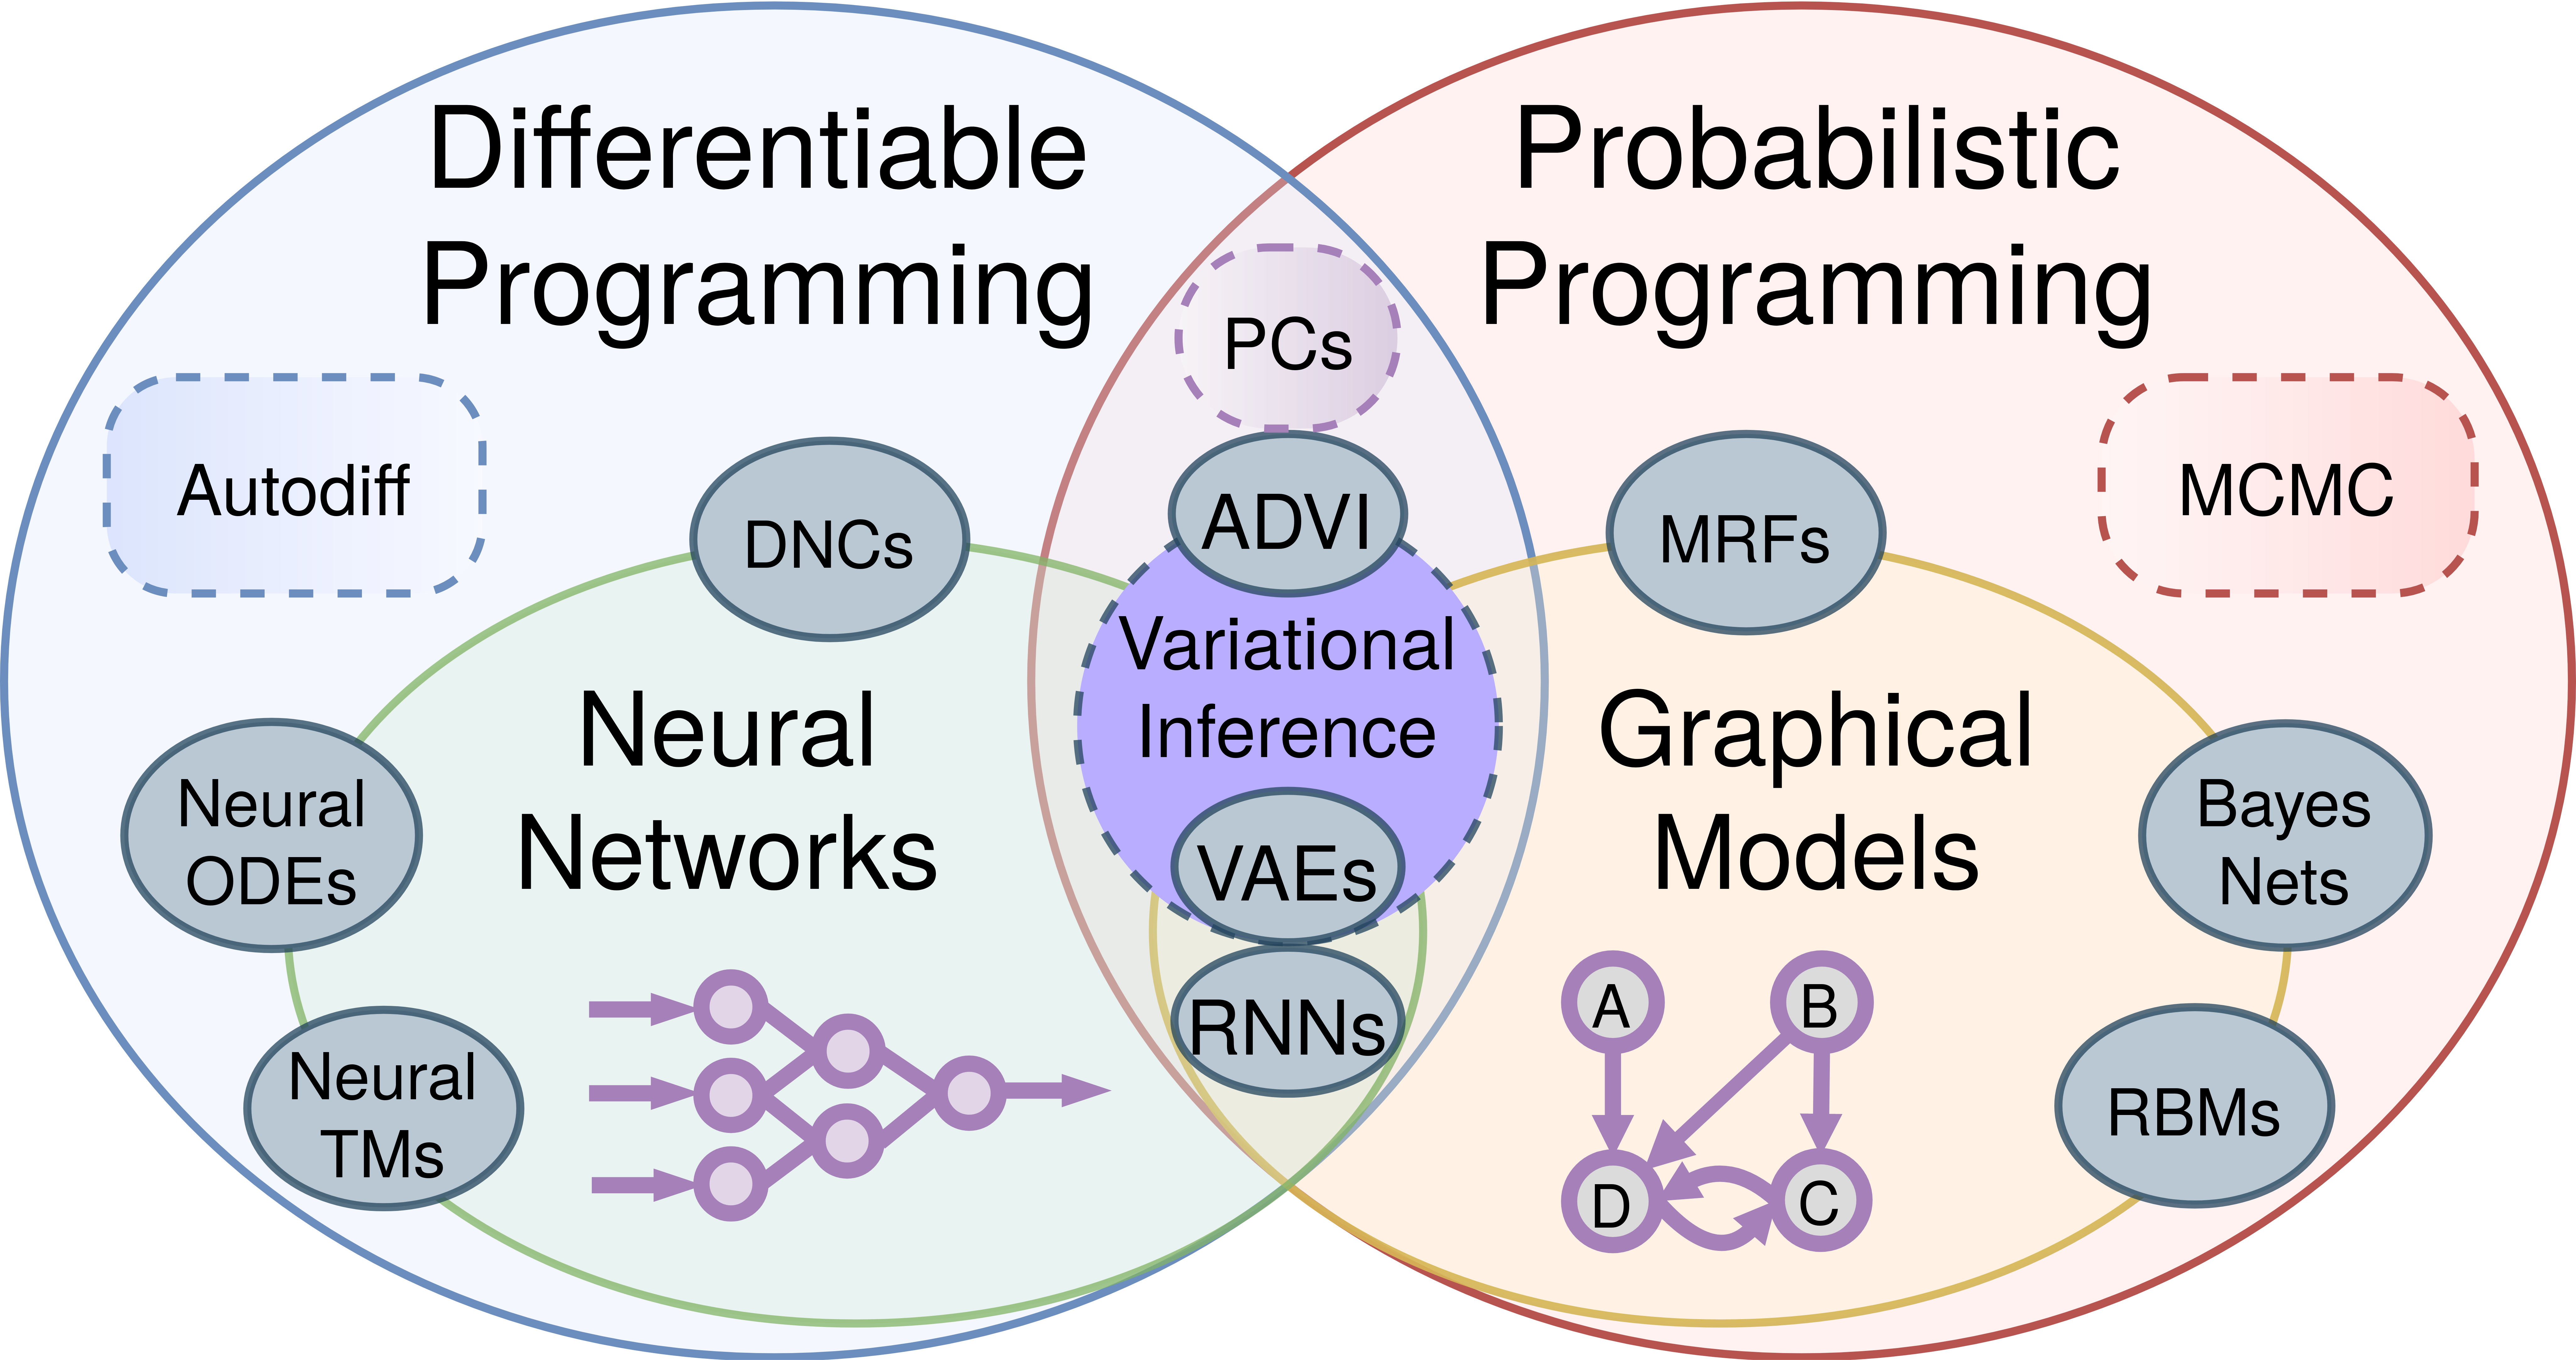
\includegraphics[width=0.90\textwidth]{../figures/diff_prob_prog.png}
    \caption{\textit{Differentiable programming} includes neural networks, but more broadly, arbitrary programs which use automatic differentiation and gradient-based optimization to approximate a loss function. \textit{Probabilistic programming}~\citep{carpenter2017stan, gorinova2018slicstan} is a generalization of probabilistic graphical models which uses Markov chain Monte Carlo (MCMC) and differentiable inference to approximate a probability density function.}
    \label{fig:diff_prob_prog}
\end{figure}

The renaissance of modern deep learning is widely attributed to progress in three research areas: algorithms, data and hardware. Among algorithms, most research has focused on deep learning architectures and representation learning. Equally important, arguably, is the role that automatic differentiation (AD) has played in facilitating the implementation of these ideas. Prior to the advent of general-purpose AD libraries such as \href{http://deeplearning.net/software/theano/}{Theano}, \href{https://pytorch.org/}{PyTorch} and \href{https://tensorflow.org/}{TensorFlow}, gradients had to be derived manually. The widespread adoption of AD software simplified and accelerated the pace of gradient-based machine learning, allowing researchers to build deeper network architectures and new learning representations. Some of these ideas in turn, formed the basis for new methods in AD, which continues to be an \href{http://www.autodiff.org}{active area} of research in the programming language and scientific computing communities.

A key aspect of the connectionist paradigm is gradient descent of a statistical loss function defined on a neural network with respect to its free parameters. For gradient descent to work, the representation must be differentiable almost everywhere. However, many representations are non-differentiable in their natural domain. For example, the structure of written language is not easily differentiable, as small changes to a word's symbolic form can cause sudden changes to its semantics~\citep{vanmerrienboer2018phd}. A key insight from representation learning is that many discrete data types can be mapped into a smoother latent space. For example, if we represent words as a vector of real numbers, $\mathbb R^N$, then it is possible to learn a mapping from words to $\mathbb R^N$ so that semantic relations between words (as defined by their statistical co-occurrence in large corpora) are geometrically preserved in vector space~\citep{pennington2014glove} -- words with similar meanings map to similar vectors. Many classes of discrete problems can be relaxed to continuous surrogates by learning such representations, or \textit{embeddings} in an unsupervised, or semi-supervised manner.

Around the same time, the deep learning community realized that perhaps strict differentiability was not so important all along. It was shown in practice, that computers using 8-bit floating point~\citep{wang2018training} and integer~\citep{wu2018training, jacob2018quantization} arithmetic are able to train neural networks without sacrificing performance. Strong assumptions like Lipschitz-continuity and $\beta$-smoothness once thought to be indispensable for gradient-based learning could be relaxed, as long as the noise introduced by quantization was negligible compared to stochastic gradient methods. In hindsight, this should have been less surprising, since all digital computers use discrete representations anyway and were capable of training neural networks for nearly half a century. This suggests strict differentiability was not as important as having a good metric. As long as the loss surface permits metric learning, gradient descent is surprisingly resilient to quantization.

As deep learning solved problems across various domains, researchers observed that neural networks were part of a broader class of differentiable architectures that could be designed, implemented and analyzed in a manner not unlike computer programs. Hence the term \textit{differentiable programming}~\citep{olah2015neural} (DP) was born. Today, DP has many applications, from protein folding~\citep{alquraishi2018end}, to physics engines~\citep{hu2019difftaichi, de2018end, degrave2016differentiable} and graphics rendering~\citep{loper2014opendr} to meta-learning~\citep{liu2018darts}. These domains all have parameters that are tuned via gradient descent. Traditionally, handcrafted optimization algorithms were required, but given a smooth metric, DP promises to learn these parameters for a broad class of models, more or less automatically. Discrete optimization, however, remains an open question. To ``learn'' discrete relations without ad hoc embedding, additional techniques (\autoref{sec:future-work}), such as probabilistic programming, are likely needed. As seen in \autoref{fig:diff_prob_prog}, these two fields have developed many productive collaborations in recent years.

\section{Static and dynamic languages}

Most programs in machine learning and scientific computing are written in dynamic languages, such as Python. In contrast, most of the industry uses statically-typed languages~\citep{github}. According to some studies, type-related errors account for over 15\% of software bugs~\citep{gao2017type}. While the causality between defectiveness and static typing has not been conclusively established, dynamically-typed languages are seldom used for building safety-critical systems, and the majority of robotics applications~\citep{Areserio54:online} are written in statically-typed languages.

Static typing eliminates a broad class of runtime errors, allowing developers and tools to reason more carefully about the behavior of programs without needing to execute them. In addition to stronger syntax validation for general-purpose programming, a well-designed library in a strongly-typed language can eliminate domain-specific errors related to API misuse that would otherwise require documentation and code samples to avert, improving usability and reducing maintenance. Furthermore, strong type systems allow us to build more intelligent static analysis tools, which can provide relevant autocompletion, source code navigation, and earlier detection of runtime errors.

One frequent objection to using strongly-typed languages is attributed to the additional burden of manual type annotation. While early type-safe languages like C++ and Java required programmers to exhaustively annotate function and variable declarations, with judicious use of type inference in modern languages like Kotlin, Scala, Rust et al., most type signatures may be safely omitted and easily recovered from the surrounding context. Type inference enables modern languages to offer the brevity of dynamic-typed languages with the safety of static type checking.

\section{Imperative and functional languages}

Most programs today are written in the imperative style, due the prevalence of the Turing Machine and von Neumann architecture~\citep{backus2007can}. $\lambda$-calculus provides an equivalent\footnote{In the sense that the Turing Machine and $\lambda$-calculus are both Turing complete.} language for computing, which we argue, is a more appropriate notation for expressing mathematical functions and computing their derivatives. In imperative programming the sole purpose of using a function is to pass it values, and there is no way to refer to a function without doing so. More troubling in the case of AD, is that imperative programs have mutable state, which requires taking extra precautions when computing their derivatives.

The mathematical notion for function composition is a first-class citizen in functional programming. Just like in calculus, to take the derivative of a program composed with another program, we simply apply the chain rule (\autoref{sec:automatic-differentiation}). Since there is no mutable state in FP, no exotic data structures or compiler tricks are required.

For example, consider the vector function $f(l_1, l_2) = l_1 \cdot l_2$, seen in \autoref{fig:fp_vs_ip}. Imperative programs, by allowing mutation, are effectively destroying intermediate information. In order to recover the computation graph for reverse-mode AD, we either need to override the assignment operator, or use a tape to store the intermediate values. In pure functional programming, mutable variables do not exist, which makes our lives much easier.

\begin{figure}[t]
    \centering
    \begin{tabular}{|l|l|}
        \hline
        Imperative & Functional \\
        \hline
        {\begin{lstlisting}[style=barelisting, linewidth=5.5cm, numbers=left]
fun dot(l1, l2) {
  if (len(l1) != len(l2))
    return error
  var sum = 0
  for(i in 0 to len(l1))
    sum += l1[i] * l2[i]
  return sum
}
        \end{lstlisting}}
         &
        {\begin{lstlisting}[style=barelisting, linewidth=6.1cm, numbers=none]
fun dot(l1, l2) {
  return if (len(l1) != len(l2))
    error
  else if (len(l1) == 0) 0
  else
    head(l1) * head(l2) +
    dot(tail(l1), tail(l2))
}
        \end{lstlisting}}
        \\
        \hline
    \end{tabular}
    \caption{Two equivalent programs, both implementing the function $f(l_1, l_2) = l_1 \cdot l_2$.}
    \label{fig:fp_vs_ip}
\end{figure}

Functional programming lets Kotlin$\nabla$ use the same abstraction for representing mathematical functions and programming functions. All functions in Kotlin$\nabla$ are pure functions, composed of expressions forming a data-flow graph (DFG). An expression is simply a \inline{Function}, which is only evaluated when invoked with numerical values, e.g. \inline{z(0, 0)}. In this way, Kotlin$\nabla$ is similar to other graph-based frameworks like \href{https://www.tensorflow.org/guide/graphs}{TensorFlow} and \href{http://deeplearning.net/software/theano/extending/graphstructures.html}{Theano}.

\section{Kotlin}\label{sec:kotlin}

When programming in a statically-typed language, a common question one might ask the compiler is, ``Given a value, \inline{x}, can \inline{x} be assigned to a variable of type \inline{Y}?'' (e.g. type checking \inline{x instanceof Y}) In Java, this question turns out to be \href{http://io.livecode.ch/learn/namin/unsound}{ill-posed}~\citep{amin2016java} and undecidable~\citep{grigore2017java} in the general case. It is possible to construct a Java program in which the answer is ``yes'' regardless of \inline{Y}, or for which an answer cannot always be determined in finite time. Undecidability is not necessarily a showstopper, but Java's unsoundness is more critical and unclear how to fix, even though it rarely occurs in practice.

Kotlin is a statically-typed language that is well-suited for building cross-platform applications, with compiler support for JVM, JavaScript and native targets. Unlike most programming languages, Kotlin was designed with IDE support from the outset, and has gained some traction in the JVM ecosystem due to its ergonomics. Kotlin's type system~\citep{tate2013mixed} is strictly \href{https://kotlinlang.org/docs/reference/generics.html#variance}{less expressive}, but fully interoperable with Java's. It is unknown whether the same issues which affect Java's type system are present in Kotlin's, but interoperability with Java has broadened its adoption and remains a key usability feature of the language.

In this work, we make use of several language features unique to Kotlin, such as first-class functions (\autoref{sec:first-class-functions}), extension functions (\autoref{sec:extension-functions}), operator overloading (\autoref{sec:operator-overloading}), and algebraic data types (\autoref{sec:adts}). Furthermore, we make heavy use of Kotlin's \href{https://kotlinlang.org/docs/reference/type-safe-builders.html}{DSL support} to implement shape-safe array programming. Together, these language features provide a concise, flexible and type-safe platform for mathematical programming.

\section{Kotlin\textorpdfstring{$\nabla$}}\label{sec:kotlingrad}

Prior work has demonstrated the possibility of encoding a deterministic context free (DCF) language in the Java type system as a \textit{fluent interface}~\citep{gil2016formal, nakamaru2017silverchain}. This result was strengthened to prove Java's type system is Turing complete (TC)~\citep{grigore2017java}, which enables us to perform shape checking and inference on array programs written in Java. Kotlin is a Java descendant which is at least DCF at the type level. Kotlin$\nabla$, an embedded DSL in the Kotlin language is TC at the value level and DCF at the type level. A similar approach is feasible in most languages with generic types.

Differentiable programming has a rich history among dynamic languages like Python, Lua and JavaScript, with early implementations including projects like \href{http://deeplearning.net/software/theano/}{Theano}~\citep{bergstra2010theano}, \href{http://torch.ch/}{Torch}~\citep{collobert2002torch}, and \href{https://tensorflow.org/}{TensorFlow}~\citep{abadi2016tensorflow}. Similar ideas have been implemented in functional languages such as Scheme (\href{https://github.com/Functional-AutoDiff/STALINGRAD}{Stalin$\nabla$}~\citep{pearlmutter2008using}), and statically-typed languages like F\# (\href{https://diffsharp.github.io/DiffSharp/}{DiffSharp}~\citep{baydin2015diffsharp}) and \href{https://www.tensorflow.org/swift}{Swift}~\citep{lattner2018tensorflow}. However, the majority of existing automatic differentiation (AD) libraries use a loosely-typed DSL, and few offer shape-safe tensor operations in a widely-used programming language.

Existing AD implementations for the JVM include \href{https://feiwang3311.github.io/Lantern/}{Lantern}~\citep{wang2018demystifying}, \href{https://tongfei.me/nexus/}{Nexus}~\citep{chen2017typesafe} and \href{https://github.com/ThoughtWorksInc/DeepLearning.scala}{DeepLearning.scala}~\citep{yang2018dl4s}, however these are Scala-based and do not interoperate with other JVM languages. Kotlin$\nabla$ is fully interoperable with vanilla Java, enabling broader adoption in neighboring languages. To our knowledge, Kotlin has no prior AD implementation. However, the language has several useful features for implementing a native AD framework. Kotlin$\nabla$ primarily relies on the following language features:

\begin{itemize}
\item \textbf{Operator overloading and infix functions} allow a concise notation for defining arithmetic operations on tensor-algebraic structures, i.e.\ groups, rings and fields.
\item \textbf{$\mathbf{\lambda}$-functions} support functional programming, following~\citet{pearlmutter2008reverse, pearlmutter2008using, siskind2008nesting, elliott2009beautiful, elliott2018simple}, et al.
\item \textbf{Extension functions} support extending classes with new fields and methods which can be exposed to external callers without requiring sub-classing or inheritance.
\end{itemize}

\begin{figure}
    \centering
    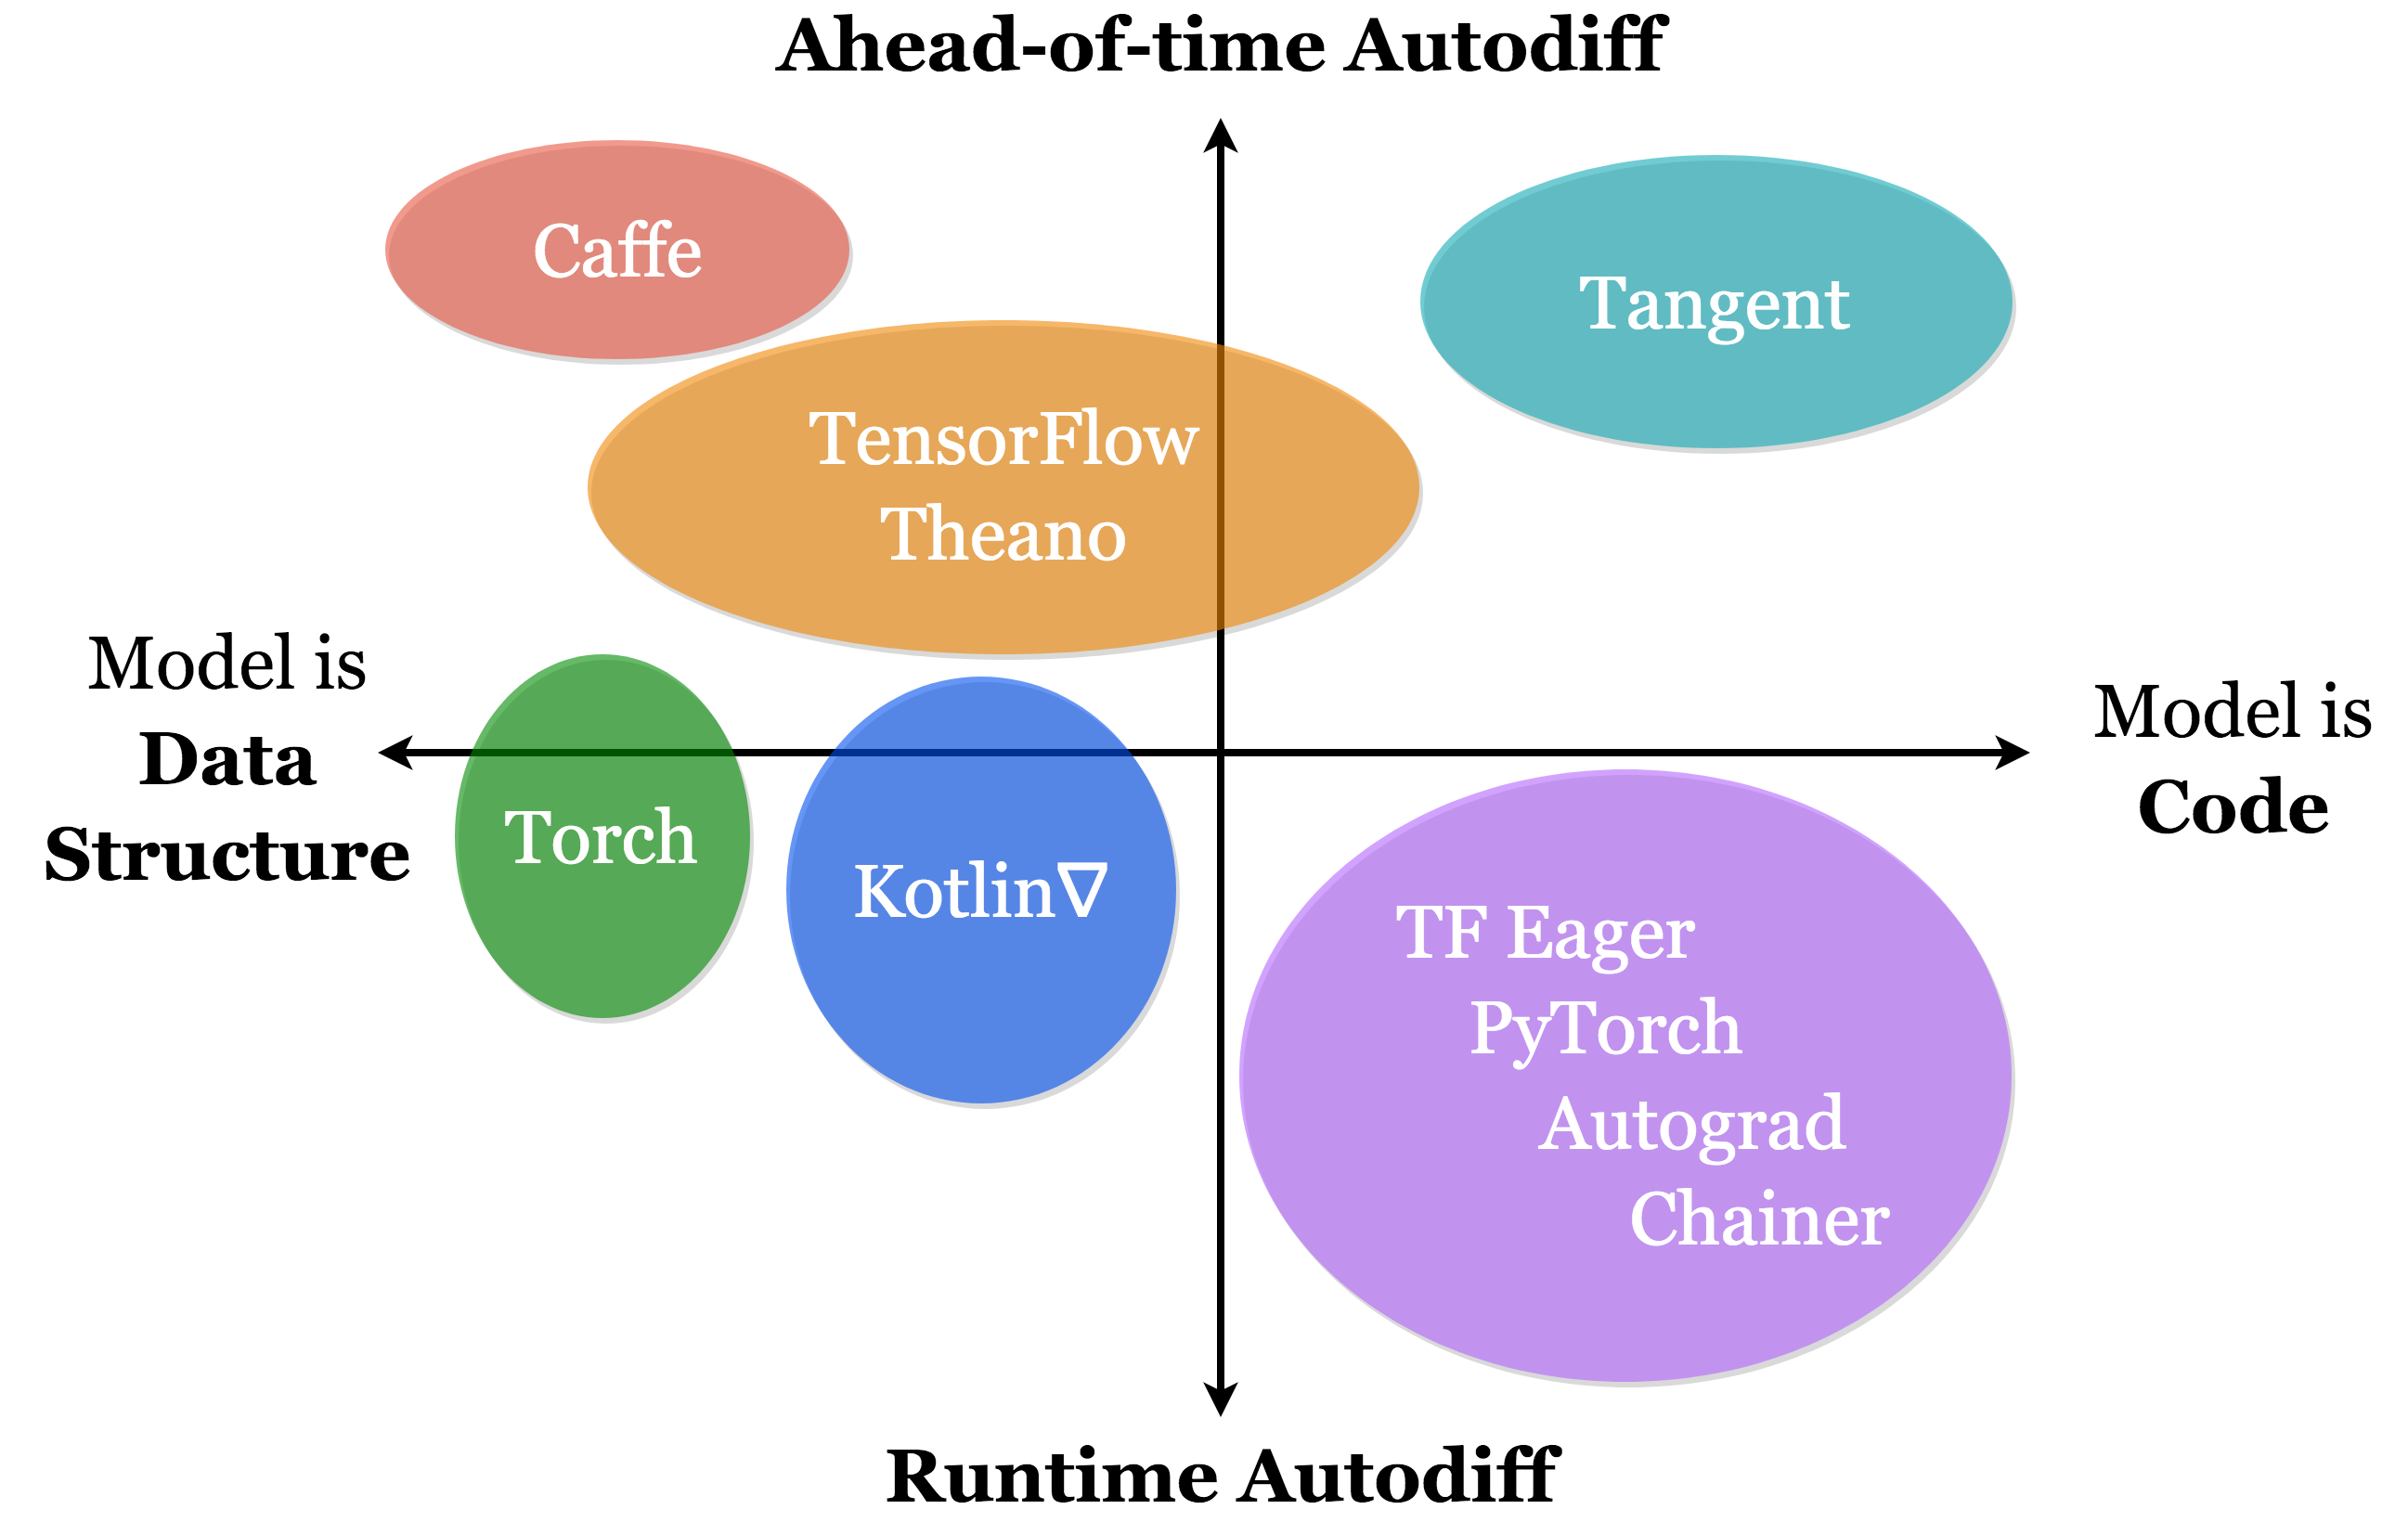
\includegraphics[width=0.70\textwidth]{../figures/kotlingrad_diagram.png}
    \caption{Adapted from~\citet{van2018tangent}. Kotlin$\nabla$ models are data structures, constructed by an embedded DSL, eagerly optimized, and lazily evaluated.}
    \label{fig:kotlingrad_digram}
\end{figure}

Kotlin$\nabla$ models are embedded domain-specific languages (eDSLs). These languages may look and act different from the host language, but are really just carefully disguised functions for building an abstract syntax tree (AST). Often these ASTs represent simple state machines, but are also used to embed a programming language. Popular examples include \href{https://docs.microsoft.com/en-us/dotnet/framework/data/adonet/sql/linq/}{SQL/LINQ}~\citep{meijer2006linq}, \href{http://stanford-ppl.github.io/Delite/optiml/}{OptiML}~\citep{sujeeth2011optiml} and other fluent interfaces~\citep{fowler05fluent}. In a sufficiently expressive host language, one can implement any language as a library, without the need to write a lexer, parser, compiler or interpreter. And with proper typing, users will receive code completion and static analysis from their favorite developer tools. Functional languages are often suitable host languages~\citep{elliott2003compiling,rompf2010lightweight}, perhaps owing to the notion of code as data.

\section{Usage}

Kotlin$\nabla$ allows users to implement differentiable programs by composing expressions. Consider the following Kotlin$\nabla$ program with two inputs and one output:
%
\begin{figure}[H] \label{fig:basic_kotlingrad}
\begin{unbreakablekotlin}
with(DoublePrecision) { // Uses double precision numerics for evaluation
  val x = Var("x") // Declare immutable variables (these variables are
  val y = Var("y") // just symbolic constructs used for differentiation)
  val z = sin(10 * (x * x + pow(y, 2))) / 10 // Lazily evaluated
  val dz_dx = d(z) / d(x) // Supports Leibniz notation(*~\citep{christianson2012leibniz}*)
  val d2z_dxdy = d(dz_dx) / d(y) // Mixing higher order partials
  val d3z_d2xdy = grad(d2z_dxdy)[x] // Equivalent to d(f)/d(x)
  plot3D(d3z_d2xdy, -1.0, 1.0) // Plot in 3-space (-1 < x, y, z < 1)
}
\end{unbreakablekotlin}
%    \centering $z = \sin{\big(10(x*x + y^2)\big)} / 10$, \texttt{plot}$\Big\left(\frac{\partial^{3z}}{\partial{x^2}\partial{y}}\Big\right)$ \\
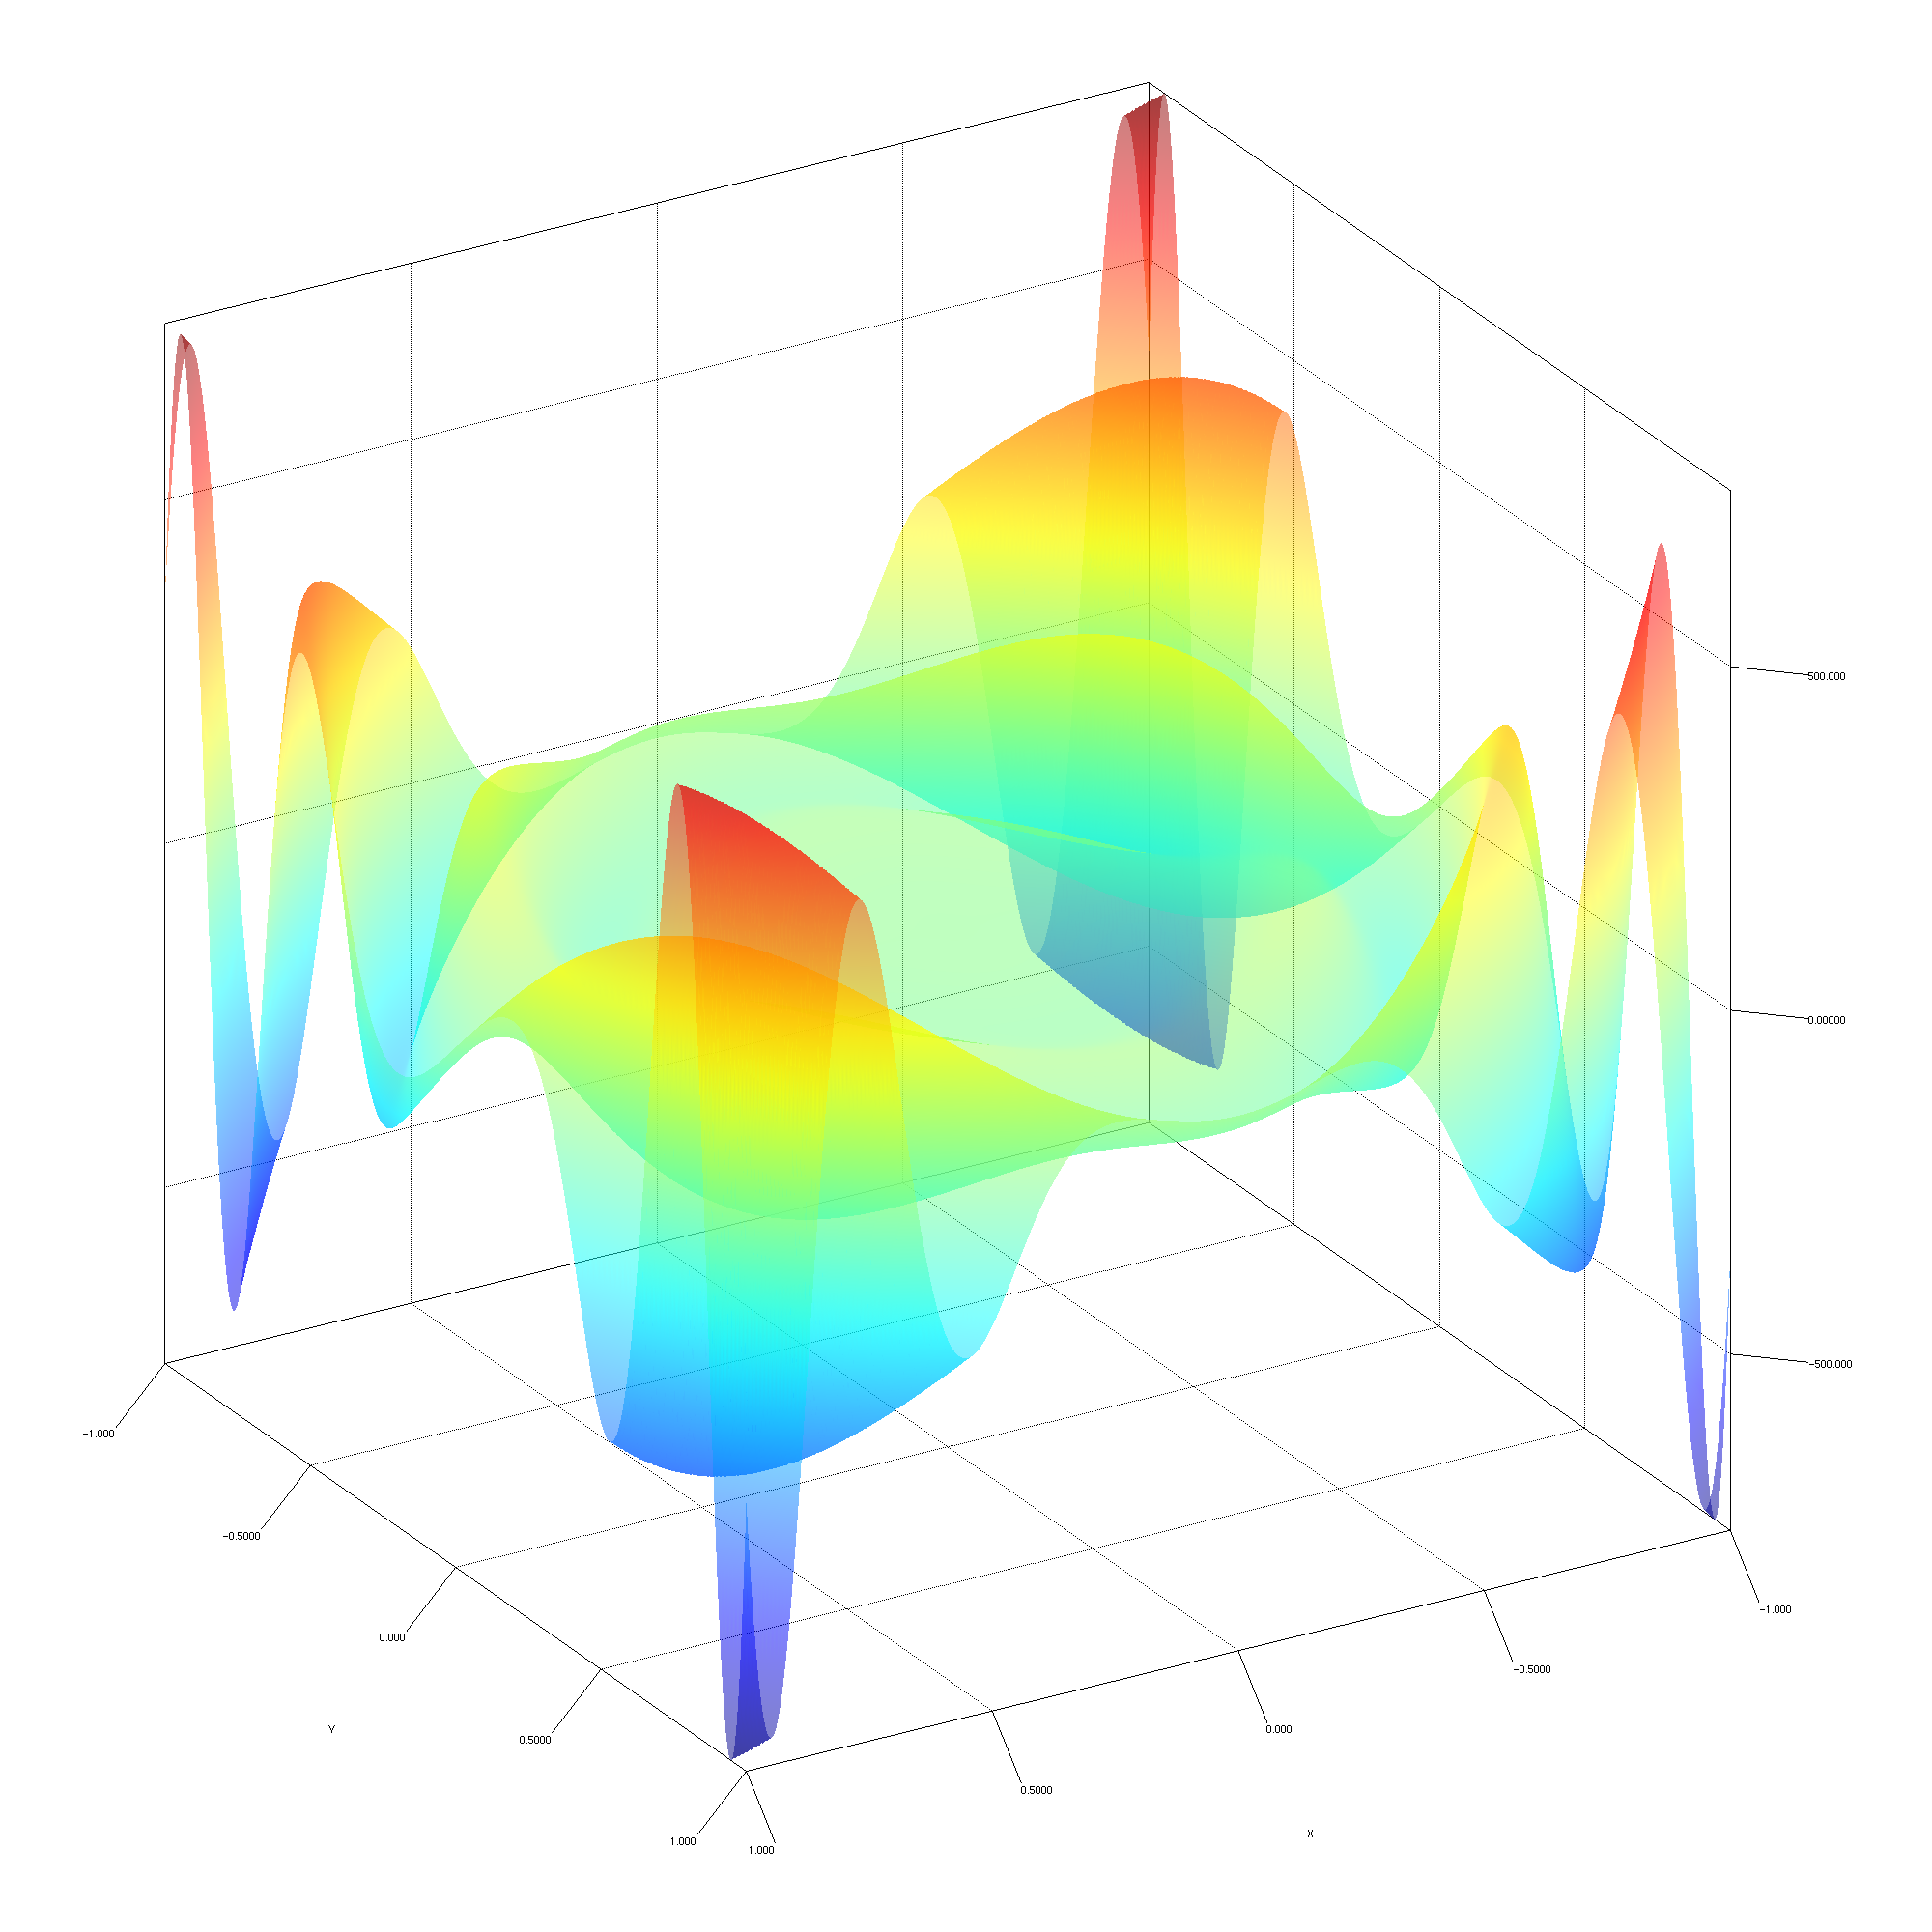
\includegraphics[scale=0.43]{../figures/plot_result.png}
\end{figure}
%
Above, we define a function with two variables and take a series of partial derivatives with respect to each variable. Expressions are lazily evaluated inside a numerical context, which may be imported on a per-file basis or lexically scoped for finer-grained control over the runtime behavior. The function is numerically evaluated on the interval $(-1, 1)$ in each dimension and rendered in 3-space.
% We can also plot higher dimensional manifolds (e.g.\ the loss surface of a neural network), projected into four dimensions, and rendered in three, where one axis is represented by time.
%
\begin{figure}
%\begin{unbreakablekotlin}
%val z = sin(10 * (x * x + pow(y, 2))) / 10 // Does not perform calculation
%\end{unbreakablekotlin}
\begin{unbreakablekotlin}
val t = (1 + x * 2 + z / y).d(y).d(x) + z / y * 3 - 4 * (y pow y).d(y)
\end{unbreakablekotlin}
\end{figure}
\vspace{-40pt}
\begin{figure}
\centering
%\begin{tikzpicture}[grow=left]
%    \tikzset{level distance=60pt}
%    \Tree [.$\div$ [.\inline{sin} [.$\times$ \inline{10} [.$+$ [.$\times$ \inline{\textbf{x}} \inline{\textbf{x}} ] [.\inline{pow} \inline{\textbf{y}} \inline{2} ] ] ] ] \inline{10} ]
%\end{tikzpictre}
%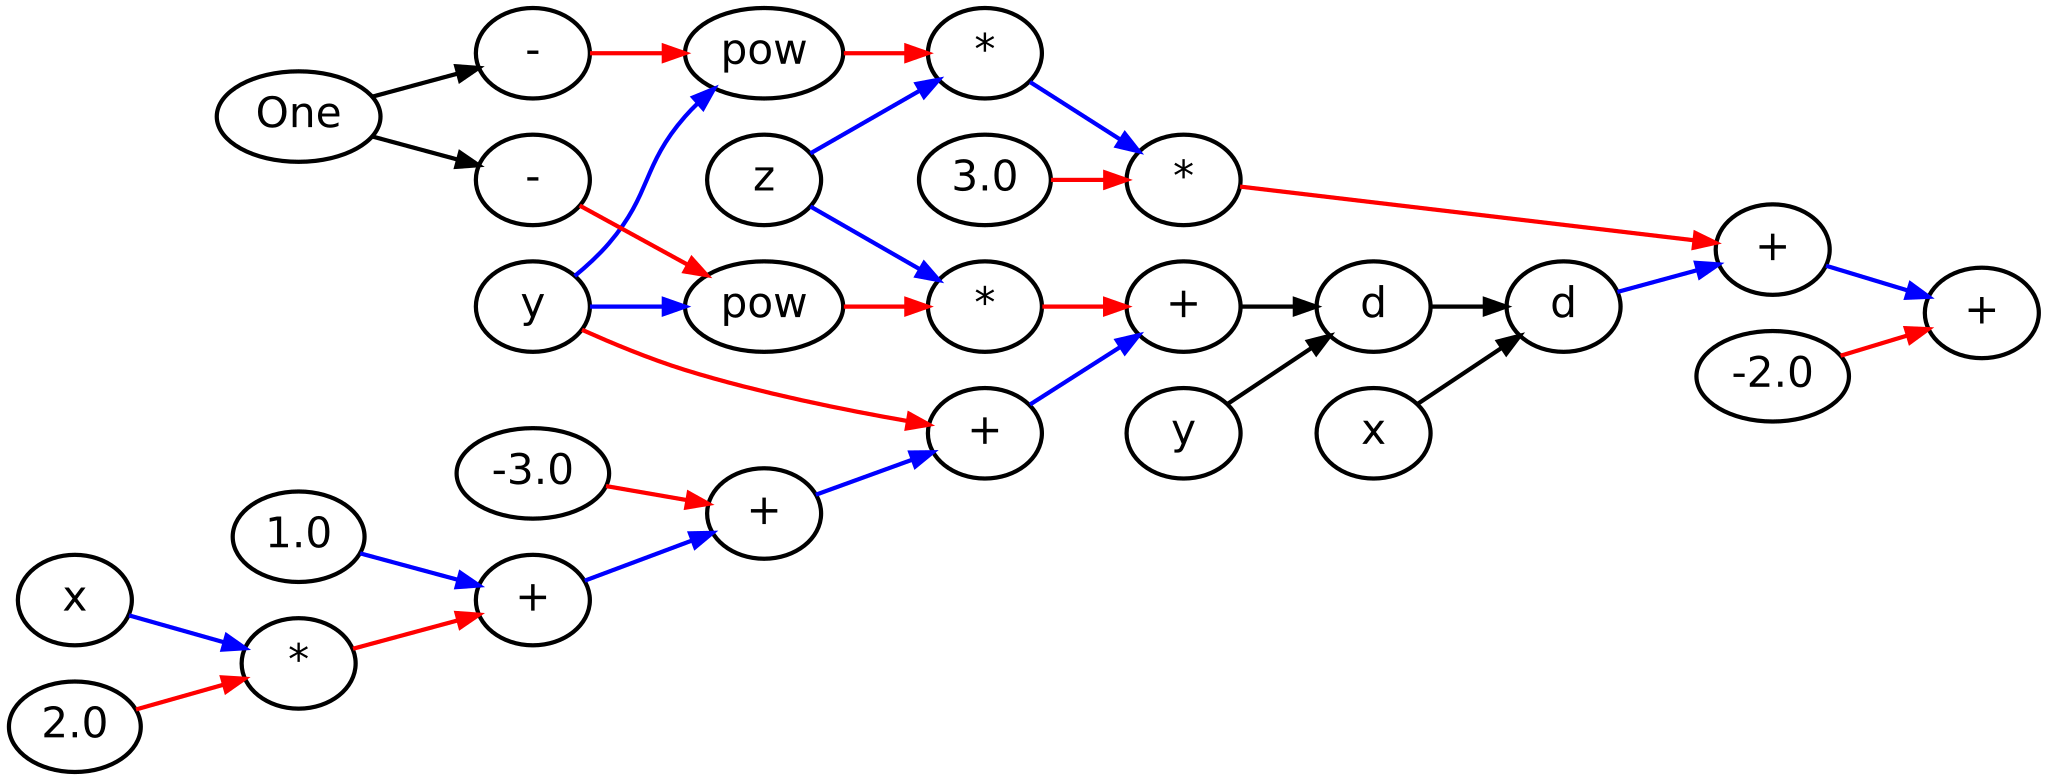
\includegraphics[scale=0.60]{../figures/dataflow.png}
\digraph[scale=0.5]{abc} {
graph ["rankdir"="LR","bgcolor"="transparent"];
"209813603" ["color"="black","fontcolor"="black","fontname"="Helvetica","fontsize"="20","style"="setlinewidth(2)","label"="+"];
"659748578" ["color"="black","fontcolor"="black","fontname"="Helvetica","fontsize"="20","style"="setlinewidth(2)","label"="+"];
"483422889" ["color"="black","fontcolor"="black","fontname"="Helvetica","fontsize"="20","style"="setlinewidth(2)","label"="d"];
"1277181601" ["color"="black","fontcolor"="black","fontname"="Helvetica","fontsize"="20","style"="setlinewidth(2)","label"="d"];
"488970385" ["color"="black","fontcolor"="black","fontname"="Helvetica","fontsize"="20","style"="setlinewidth(2)","label"="+"];
"93122545" ["color"="black","fontcolor"="black","fontname"="Helvetica","fontsize"="20","style"="setlinewidth(2)","label"="+"];
"1239731077" ["color"="black","fontcolor"="black","fontname"="Helvetica","fontsize"="20","style"="setlinewidth(2)","label"="1.0"];
"249515771" ["color"="black","fontcolor"="black","fontname"="Helvetica","fontsize"="20","style"="setlinewidth(2)","label"="*"];
"x" ["color"="black","fontcolor"="black","fontname"="Helvetica","fontsize"="20","style"="setlinewidth(2)"];
"1627960023" ["color"="black","fontcolor"="black","fontname"="Helvetica","fontsize"="20","style"="setlinewidth(2)","label"="2.0"];
"1811044090" ["color"="black","fontcolor"="black","fontname"="Helvetica","fontsize"="20","style"="setlinewidth(2)","label"="*"];
"z" ["color"="black","fontcolor"="black","fontname"="Helvetica","fontsize"="20","style"="setlinewidth(2)"];
"940060004" ["color"="black","fontcolor"="black","fontname"="Helvetica","fontsize"="20","style"="setlinewidth(2)","label"="*"];
"1945604815" ["color"="black","fontcolor"="black","fontname"="Helvetica","fontsize"="20","style"="setlinewidth(2)","label"="*"];
"328638398" ["color"="black","fontcolor"="black","fontname"="Helvetica","fontsize"="20","style"="setlinewidth(2)","label"="pow"];
"y" ["color"="black","fontcolor"="black","fontname"="Helvetica","fontsize"="20","style"="setlinewidth(2)"];
"1121172875" ["color"="black","fontcolor"="black","fontname"="Helvetica","fontsize"="20","style"="setlinewidth(2)","label"="pow"];
"1644443712" ["color"="black","fontcolor"="black","fontname"="Helvetica","fontsize"="20","style"="setlinewidth(2)","label"="pow"];
"745160567" ["color"="black","fontcolor"="black","fontname"="Helvetica","fontsize"="20","style"="setlinewidth(2)","label"="d"];
"391447681" ["color"="black","fontcolor"="black","fontname"="Helvetica","fontsize"="20","style"="setlinewidth(2)","label"="*"];
"1308927845" ["color"="black","fontcolor"="black","fontname"="Helvetica","fontsize"="20","style"="setlinewidth(2)","label"="-"];
"440434003" ["color"="black","fontcolor"="black","fontname"="Helvetica","fontsize"="20","style"="setlinewidth(2)","label"="-"];
"1" ["color"="black","fontcolor"="black","fontname"="Helvetica","fontsize"="20","style"="setlinewidth(2)","label"="One"];
"1595953398" ["color"="black","fontcolor"="black","fontname"="Helvetica","fontsize"="20","style"="setlinewidth(2)","label"="-"];
"1277181601{color=black, fontcolor=black, fontname=Helvetica, fontsize=20, style=setlinewidth(2)}->" ["color"="black","fontcolor"="black","fontname"="Helvetica","fontsize"="20","style"="setlinewidth(2)","label"="y"];
"483422889{color=black, fontcolor=black, fontname=Helvetica, fontsize=20, style=setlinewidth(2)}->" ["color"="black","fontcolor"="black","fontname"="Helvetica","fontsize"="20","style"="setlinewidth(2)","label"="x"];
"1684106402" ["color"="black","fontcolor"="black","fontname"="Helvetica","fontsize"="20","style"="setlinewidth(2)","label"="3.0"];
"403424356" ["color"="black","fontcolor"="black","fontname"="Helvetica","fontsize"="20","style"="setlinewidth(2)","label"="4.0"];
"745160567{color=black, fontcolor=black, fontname=Helvetica, fontsize=20, style=setlinewidth(2)}->" ["color"="black","fontcolor"="black","fontname"="Helvetica","fontsize"="20","style"="setlinewidth(2)","label"="y"];
"659748578" -> "209813603" ["color"="blue","arrowhead"="normal","style"="setlinewidth(2)"];
"483422889" -> "659748578" ["color"="blue","arrowhead"="normal","style"="setlinewidth(2)"];
"1277181601" -> "483422889" ["color"="black","arrowhead"="normal","style"="setlinewidth(2)"];
"488970385" -> "1277181601" ["color"="black","arrowhead"="normal","style"="setlinewidth(2)"];
"93122545" -> "488970385" ["color"="blue","arrowhead"="normal","style"="setlinewidth(2)"];
"1239731077" -> "93122545" ["color"="blue","arrowhead"="normal","style"="setlinewidth(2)"];
"249515771" -> "93122545" ["color"="red","arrowhead"="normal","style"="setlinewidth(2)"];
"x" -> "249515771" ["color"="blue","arrowhead"="normal","style"="setlinewidth(2)"];
"1627960023" -> "249515771" ["color"="red","arrowhead"="normal","style"="setlinewidth(2)"];
"1811044090" -> "488970385" ["color"="red","arrowhead"="normal","style"="setlinewidth(2)"];
"z" -> "1811044090" ["color"="blue","arrowhead"="normal","style"="setlinewidth(2)"];
"z" -> "940060004" ["color"="blue","arrowhead"="normal","style"="setlinewidth(2)"];
"940060004" -> "1945604815" ["color"="blue","arrowhead"="normal","style"="setlinewidth(2)"];
"1945604815" -> "659748578" ["color"="red","arrowhead"="normal","style"="setlinewidth(2)"];
"328638398" -> "1811044090" ["color"="red","arrowhead"="normal","style"="setlinewidth(2)"];
"y" -> "328638398" ["color"="blue","arrowhead"="normal","style"="setlinewidth(2)"];
"y" -> "1121172875" ["color"="blue","arrowhead"="normal","style"="setlinewidth(2)"];
"y" -> "1644443712" ["color"="blue","arrowhead"="normal","style"="setlinewidth(2)"];
"y" -> "1644443712" ["color"="red","arrowhead"="normal","style"="setlinewidth(2)"];
"1121172875" -> "940060004" ["color"="red","arrowhead"="normal","style"="setlinewidth(2)"];
"1644443712" -> "745160567" ["color"="black","arrowhead"="normal","style"="setlinewidth(2)"];
"745160567" -> "391447681" ["color"="red","arrowhead"="normal","style"="setlinewidth(2)"];
"391447681" -> "1308927845" ["color"="black","arrowhead"="normal","style"="setlinewidth(2)"];
"1308927845" -> "209813603" ["color"="red","arrowhead"="normal","style"="setlinewidth(2)"];
"440434003" -> "328638398" ["color"="red","arrowhead"="normal","style"="setlinewidth(2)"];
"1" -> "440434003" ["color"="black","arrowhead"="normal","style"="setlinewidth(2)"];
"1" -> "1595953398" ["color"="black","arrowhead"="normal","style"="setlinewidth(2)"];
"1595953398" -> "1121172875" ["color"="red","arrowhead"="normal","style"="setlinewidth(2)"];
"1277181601{color=black, fontcolor=black, fontname=Helvetica, fontsize=20, style=setlinewidth(2)}->" -> "1277181601" ["color"="black","arrowhead"="normal","style"="setlinewidth(2)"];
"483422889{color=black, fontcolor=black, fontname=Helvetica, fontsize=20, style=setlinewidth(2)}->" -> "483422889" ["color"="black","arrowhead"="normal","style"="setlinewidth(2)"];
"1684106402" -> "1945604815" ["color"="red","arrowhead"="normal","style"="setlinewidth(2)"];
"403424356" -> "391447681" ["color"="blue","arrowhead"="normal","style"="setlinewidth(2)"];
"745160567{color=black, fontcolor=black, fontname=Helvetica, fontsize=20, style=setlinewidth(2)}->" -> "745160567" ["color"="black","arrowhead"="normal","style"="setlinewidth(2)"];
}
\caption{Implicit DFG constructed by the original expression, shown above.}
\label{lst:edsl}
\end{figure}\\\\

\section{Type systems}\label{sec:type-systems}

Early work in type-safe dimension analysis can be found in \citet{kennedy1994dimension, kennedy1996programming} which uses types to encode dimensionality and prevent common bugs related to dimension mismatch from arising, and was later realized in the F\# language~\citep{kennedy2010types}. \citet{jay1996shape}, \citet{rittri1995dimension}, and \citet{zenger1997indexed} explore the application of dimension types for linear algebra. More recently, \citet{kiselyov2005number, kiselyov2010fun} and \citet{griffioen2015type}, show how to manipulate arrays in more complex ways. With the resurgence of interest in tensor algebra and array programming, \citet{chen2017typesafe} and \citet{rink2018modeling} demonstrate how to encode shape-safety for tensor algebra in various type systems.

The problem we attempt to solve can be summarized as follows. Given two values \inline{x} and \inline{y}, and operator \inline{\$}, how do we determine whether the expression \inline{z = x \$ y} is valid, and if so, what is the result type of \inline{z}? For matrix multiplication, when \inline{x} $\in \mathbb{R}^{m \times n}$ and \inline{y} $\in \mathbb{R}^{n \times p}$, the expression is well-typed and we can infer \inline{z} $\in \mathbb{R}^{m \times p}$. More generally, we would like to infer the type of \inline{z} for some operator \inline{@} $: (\mathbb{R}^\mathbf{a}, \mathbb{R}^\mathbf{b}) \rightarrow \mathbb{R}^\mathbf{c}$ where $\mathbf{a} \in \mathbb{N}^q, \mathbf{b} \in \mathbb{N}^r, \mathbf{c} \in \mathbb{N}^s$ and $q, r, s \in \mathbb{N}$. For many linear algebra operations such as matrix multiplication, $\mathcal{T}(\mathbf a, \mathbf b) \stackrel{?}{=} \mathbf c$ is computable in $\mathcal{O}(1)$ -- we can simply check the inner dimensions for equivalence ($\mathbf{a}_2 \stackrel{?}{=} \mathbf{b}_1$).

Shape checking operations on multidimensional arrays is not always decidable. For arbitrary type functions $\mathcal{T}(\mathbf{a}, \mathbf{b})$, checking $\mathcal{T}(\mathbf{a}, \mathbf{b}) \stackrel{?}{=} \mathbf{c}$ requires a Turing machine. If $\mathcal{T}$ is allowed to use the multiplication operator, as in the case of convolutional arithmetic~\citep{dumoulin2016guide}, shape inference becomes equivalent to Peano arithmetic, which is undecidable~\citep{godel1931formal}. Addition, subtraction, indexing and comparison of integers are all decidable operations in Presburger arithmetic~\citep{suzuki1980verification, bradley2006decidable, charlier2011enumeration}. Equality checking is trivially decidable, and can be implemented in most static type systems.

Evaluating an arbitrary $\mathcal{T}$ which uses multiplication or division (e.g.\ convolutional arithmetic) requires a dependently typed language~\citep{xi1998eliminating, pineyro2019structure}, but checking shape equality (e.g. ordinary arithmetic) is feasible in Java and its cousins.\hspace{-.08em}\footnote{Java's type system is known to be Turing complete~\citep{grigore2017java}. Thus, emulation of dependent types in Java is theoretically possible, but likely intractable due to the practical limitations noted by Grigore.} Furthermore, we believe that shape checking ordinary matrix arithmetic is decidable in any type system loosely based on System F${}_{<:}$~\citep{cardelli1991extension}. We propose a type system for enforcing shape-safety which can be implemented in any language with subtyping and generics, such as \href{https://docs.oracle.com/javase/tutorial/java/generics/index.html}{Java}~\citep{naftalin2007java}, \href{https://kotlinlang.org/docs/reference/generics.html}{Kotlin}~\citep{tate2013mixed}, \href{https://www.typescriptlang.org/docs/handbook/advanced-types.html}{TypeScript}~\citep{bierman2014understanding} or \href{https://doc.rust-lang.org/1.7.0/book/generics.html}{Rust}~\citep{crozet2019nalgebra}.

{\tiny
\begin{table}
    \begin{tabular}{|c|c|c|c|l|}
        \hline
        \multicolumn{1}{|c|}{Math}                             &  Infix                                                                           & Prefix                                                                                    & Postfix                                                                                      & Operator Type Signature                                                                                                                                                                                      \\ \hline
                 $A(B)$                                        & \tinline{a(b)}                                                                   &                                                                                           &                                                                                              & $ (\texttt{a}:  \mathbb{R}^{\tau}\rightarrow\mathbb{R}^{\pi}, \texttt{b}: \mathbb{R}^{\lambda} \rightarrow \mathbb{R}^{\tau}) \rightarrow (\mathbb{R}^{\lambda}\rightarrow \mathbb{R}^{\pi})               $ \\ \hline
                 $A\pm B$                                      & \begin{tabular}{@{}c@{}}\tinline{a + b}\\\tinline{a - b}\end{tabular}            & \begin{tabular}{@{}c@{}}\tinline{plus(a, b)}\\\tinline{minus(a, b)}\end{tabular}          &                                                                                              & $ (\texttt{a}:  \mathbb{R}^{\tau}\rightarrow\mathbb{R}^{\pi}, \texttt{b}: \mathbb{R}^{\lambda} \rightarrow \mathbb{R}^{\pi}) \rightarrow (\mathbb{R}^{?}\rightarrow \mathbb{R}^{\pi})                      $ \\ \hline
                 $A   B$                                       & \begin{tabular}{@{}c@{}}\tinline{a * b}\\\tinline{a.times(b)}\end{tabular}       & \tinline{times(a, b)}                                                                     &                                                                                              & $ (\texttt{a}: \mathbb{R}^{\tau}\rightarrow\mathbb{R}^{m \times n}, \texttt{b}: \mathbb{R}^{\lambda}\rightarrow\mathbb{R}^{n \times p})    \rightarrow (\mathbb{R}^{?}\rightarrow\mathbb{R}^{m \times p})  $ \\ \hline
\begin{tabular}{@{}c@{}}$\frac{A}{B}$\\$AB^{-1}$\end{tabular}  & \begin{tabular}{@{}c@{}}\tinline{a / b}\\\tinline{a.div(b)}\end{tabular}         & \tinline{div(a, b)}                                                                       &                                                                                              & $ (\texttt{a}: \mathbb{R}^{\tau}\rightarrow\mathbb{R}^{m \times n}, \texttt{b}: \mathbb{R}^{\lambda}\rightarrow\mathbb{R}^{p \times n}) \rightarrow (\mathbb{R}^{?}\rightarrow\mathbb{R}^{m \times p})     $ \\ \hline
\begin{tabular}{@{}c@{}}$-A$\\$+A$\end{tabular}                &                                                                                  & \begin{tabular}{@{}c@{}}\tinline{-a}\\\tinline{+a}\end{tabular}                           & \begin{tabular}{@{}c@{}}\tinline{a.unaryMinus()}\\\tinline{a.unaryPlus()}\end{tabular}       & $                   (\texttt{a}: \mathbb{R}^{\tau}\rightarrow\mathbb{R}^{\pi}) \rightarrow (\mathbb{R}^{\tau}\rightarrow\mathbb{R}^{\pi})                                                                  $ \\ \hline
%\begin{tabular}{@{}c@{}}sin(a)\\cos(a)\\tan(a)\end{tabular}    &                                                                                  & \begin{tabular}{@{}c@{}}\tinline{sin(a)}\\\tinline{cos(a)}\\\tinline{tan(a)}\end{tabular} & \begin{tabular}{@{}c@{}}\tinline{a.sin()}\\\tinline{a.cos()}\\\tinline{a.tan()}\end{tabular} & $                                            (\texttt{a}: \mathbb{R}\rightarrow\mathbb{R}) \rightarrow (\mathbb{R}\rightarrow\mathbb{R})                                                                   $ \\ \hline
                $\ln(A)$                                       &                                                                                  & \begin{tabular}{@{}c@{}}\tinline{ln(a)}\\\tinline{log(a)}\end{tabular}                    & \begin{tabular}{@{}c@{}}\tinline{a.ln()}\\\tinline{a.log()}\end{tabular}                     & $                  (\texttt{a}: \mathbb{R}^{\tau}\rightarrow\mathbb{R}^{m \times m}) \rightarrow (\mathbb{R}^{\tau}\rightarrow\mathbb{R}^{m \times m})                                                     $ \\ \hline
               $\log_b A$                                      & \tinline{a.log(b)}                                                               & \tinline{log(a, b)}                                                                       &                                                                                              & $       (\texttt{a}: \mathbb{R}^{\tau}\rightarrow\mathbb{R}^{m \times m}, \texttt{b}: \mathbb{R}^{\lambda}\rightarrow\mathbb{R}^{m \times m}) \rightarrow (\mathbb{R}^{?}\rightarrow\mathbb{R})            $ \\ \hline
                $A^{b}$                                        & \tinline{a.pow(b)}                                                               & \tinline{pow(a, b)}                                                                       &                                                                                              & $       (\texttt{a}: \mathbb{R}^{\tau}\rightarrow\mathbb{R}^{m \times m}, \texttt{b}: \mathbb{R}^{\lambda}\rightarrow\mathbb{R}) \rightarrow (\mathbb{R}^{?}\rightarrow\mathbb{R}^{m \times m})            $ \\ \hline
\begin{tabular}{@{}c@{}}$\sqrt{a}$\\$\sqrt[3]{a}$\end{tabular} & \begin{tabular}{@{}c@{}}\tinline{a.pow(1.0/2)}\\\tinline{a.root(3)}\end{tabular} & \begin{tabular}{@{}c@{}}\tinline{a.pow(1.0/2)}\\\tinline{a.root(3)}\end{tabular}          & \begin{tabular}{@{}c@{}}\tinline{a.sqrt()}\\\tinline{a.cbrt()}\end{tabular}                  & $                        (\texttt{a}: \mathbb{R}^{\tau}\rightarrow\mathbb{R}^{m \times m}) \rightarrow (\mathbb{R}\rightarrow\mathbb{R}^{m \times m})                                                      $ \\ \hline
\begin{tabular}{@{}c@{}}$\frac{da}{db}$\\$a'(b)$\end{tabular}  & \tinline{a.d(b)}                                                                 & \tinline{grad(a)[b]}                                                                      & \tinline{d(a) / d(b)}                                                                        & $         (\texttt{a}: \mathbb{R}^{\tau}\rightarrow\mathbb{R}^{\pi}, \texttt{b}: \mathbb{R}^{\lambda}\rightarrow\mathbb{R}^{\omega}) \rightarrow (\mathbb{R}^{?}\rightarrow\mathbb{R}^{\pi \times \omega}) $ \\ \hline
    \end{tabular}
\caption{\label{tab:shape_system}Kotlin$\nabla$'s shape system specifies the output shape for tensor expressions.}
\end{table}
}
%$\dagger$ \inline{a} and \inline{b} are higher order functions. These may be constants (e.g. 0, 1.0), variables (e.g. \inline{Var("x")}) or expressions (e.g. \inline{x + 1}, \inline{2 * x + y}).

\section{Shape safety}\label{sec:shape-safety}

\noindent There are three broad strategies for handling shape errors in array programming: \\
%
\begin{enumerate}
    \item Conceal the error by implicitly reshaping or \href{https://docs.scipy.org/doc/numpy-1.15.0/user/basics.broadcasting.html}{broadcasting arrays}.
    \item Announce the error at runtime with a relevant message, e.g.~\href{https://www.tensorflow.org/api_docs/python/tf/errors/InvalidArgumentError}{\inline{InvalidArgumentError}}.
    \item Do not allow programs which can result in a shape error to compile. \\
\end{enumerate}
%
Most array programming libraries such as NumPy~\citep{van2011numpy} or TensorFlow~\citep{abadi2016tensorflow} use the first or second strategy. In Kotlin$\nabla$, we adopt the third, which allows an incremental type checker, such as those typically found in modern IDEs, to instantaneously detect when a matrix operation is invalid. Consider the following example:
%
\begin{kotlinlisting}
val vecA = Vec(1.0, 2.0)      // Inferred type: Vec<Int, D2>
val vecB = Vec(1.0, 2.0, 3.0) // Inferred type: Vec<Int, D3>
val vecC = vecB + vecB
val vecD = (*\uwave{vecA + vecB}*) // Compile error: Expected Vec<2>, found Vec<3>
\end{kotlinlisting}
%
Attempting to sum two vectors whose shapes do not match will fail to compile.
%
\begin{kotlinlisting}
val matA = Mat1x4(1.0, 2.0, 3.0, 4.0) // Inferred type: Mat<Double, D1, D4>
val matB = Mat4x1(1.0, 2.0, 3.0, 4.0) // Inferred type: Mat<Double, D4, D1>
val matC = matA * matB
val matD = (*\uwave{matA *\ matC}*) // Compile error: Expected Mat<4, *>, found Mat<1, 1>
\end{kotlinlisting}
%
Similarly, multiplying two matrices whose inner dimensions do not match will not compile.
%
\begin{kotlinlisting}
val matA = Mat2x4(1.0, 2.0, 3.0, 4.0,
                  5.0, 6.0, 7.0, 8.0)
val matB = Mat4x2(1.0, 2.0,
                  3.0, 4.0,
                  5.0, 6.0,
                  7.0, 8.0)
val matC: Mat<Double, D2, D2> = a * b // Types are optional, but encouraged
val matD = Mat2x1(1.0, 2.0)
val matE = matC * matD
val matF = Mat3x1(1.0, 2.0, 3.0)
val matG = (*\uwave{matE *\ matF}*) // Compile error: Expected Mat<1, *>, found Mat<3, 1>
\end{kotlinlisting}
%
It is required to specify the parameter types in a method signature. Explicit return types are optional but encouraged for readability. If omitted, the type system can often infer them:
%
\begin{kotlinlisting}
fun someMatFun(m: Mat<Double, D3, D1>): Mat<Double, D3, D3> = ...
fun someMatFun(m: Mat<Double, D2, D2>) = ...
\end{kotlinlisting}
%
Shape safety is currently supported up to rank-2 tensors, i.e.\ matrices. To perform dimension checking in our type system, first we enumerate a list of integer type literals as a chain of subtypes, $C <: C - 1 <: C - 2 <: \dots <: 1 <: 0$, where $C$ is the largest fixed-length dimension we wish to represent, which can be specified by the user prior to compilation. This guarantees linear space and time complexity for subtype checking, with a constant upper bound.
%
\begin{kotlinlisting}[caption={Shape safe tensor addition for rank-1 tensors, $\forall C\leq2.$}]
interface Nat<T: D0> { val i: Int }
// Integer literals have reified Int values should we need to compare them at runtime
sealed class D0(open val i: Int = 0) { companion object: D0(), Nat<D0> }
sealed class D1(override val i: Int = 1): D0(i) { companion object: D1(), Nat<D1> }
sealed class D2(override val i: Int = 2): D1(i) { companion object: D2(), Nat<D2> }
sealed class D3(override val i: Int = 3): D2(i) { companion object: D3(), Nat<D3> }
//...Code for integer literals should be generated
sealed class D99(override val i: Int = 99): D98(i) { companion object: D99(), Nat<D99> }
\end{kotlinlisting}
%
Next, we overload the call operator to emulate instantiating a collection literal, using arity to infer its dimensionality. Consider the rank-1 case for length inference on vector literals:
%
\begin{kotlinlisting}
open class Vec<E, Len: D1> constructor(val contents: List<E>) {
    companion object {
        operator fun <T> invoke(t: T): Vec<T, D1> = Vec(listOf(t))
        operator fun <T> invoke(t0: T, t1: T): Vec<T, D2> = Vec(listOf(t0, t1))
        operator fun <T> invoke(t0: T, t1: T, t2: T): Vec<T, D3> = Vec(listOf(t0, t1, t2))
    }
}
\end{kotlinlisting}
%
Finally, we overload arithmetical operators using generic shape constraints. Since our type-level integers are a chain of subtypes, we only need to define one operator and can rely on Liskov substitution~\citep{liskov1987} to preserve shape safety for all subtypes.
%
\begin{kotlinlisting}
// <C: D1> will accept 1 <= C <= 99 via Liskov substitution
operator fun <E, C: D1, V: Vec<X, C>> V.plus(v: V): V = TODO()
\end{kotlinlisting}
%
The operator \inline{+} can now be used like so. Incompatible operands will cause a type error:
%
\begin{kotlinlisting}
// Type-checked vector addition with shape inference
val Y = Vec(0, 0) + Vec(0, 0) // Y: Vec<Float, D2>
val X = (*\uwave{Vec(0, 0) + Vec(0, 0, 0)}*) // Compile error: Expected Vec<Int, D2>, found Vec<Int, D3>
\end{kotlinlisting}
%
Dynamic length construction is also permitted, although it may fail at runtime. For example:
%
\begin{kotlinlisting}
val one = Vec(0, 0, 0) + Vec(0, 0, 0) // Always runs safely
val add = Vec(0, 0, 0) + Vec<Int, D3>(listOf(...)) // Compiles, but may fail at runtime
val vec = Vec(0, 0, 0) // Inferred type: Vec<3>
val sum = (*\uwave{Vec(0, 0) + add}*) // Compile error: Expected Vec<Int, D2>, found Vec<Int, D3>
\end{kotlinlisting}
%
Matrices and tensors have a similar syntax. For example, Kotlin$\nabla$ can infer the shape of matrix multiplication, and will not compile if the arguments' inner dimensions disagree:
%
\begin{kotlinlisting}
open class Mat<X, R: D1, C: D1>(vararg val rows: Vec<X, C>)
fun <X> Mat1x2(d0: X, d1: X): Mat<X, D1, D2> = Mat(Vec(d0, d1))
fun <X> Mat2x1(d0: X, d1: X): Mat<X, D2, D1> = Mat(Vec(d0), Vec(d1))

operator fun <X, Q: D1, R: D1, S: D1> Mat<X, Q, R>.times(m: Mat<X, R, S>): Mat<X, Q, S> =
    Mt( *(rows.indices).map { i -> /* ... */ }.toTypedArray() )

val matM = Mat1x2(0, 0)
val matO = (*\uwave{matM *\ matM}*) // Compile error: Expected Mat<2, *>, found Mat<1, 2>
\end{kotlinlisting}
%
A similar technique can be found in nalgebra~\citep{crozet2019nalgebra}, a shape-checked linear algebra library for the Rust language which also uses synthetic type-level integers. This technique originates in Haskell, a language which supports more powerful forms of type-level computation, such as \textit{type arithmetic}~\citep{kiselyov2005number}. Type arithmetic simplifies array concatenation, convolutional arithmetic~\citep{dumoulin2016guide} and other operations which are currently difficult to express in Kotlin$\nabla$, where arbitrary type-level functions $\mathcal{T}(\mathbf a, \mathbf b)$ (ref.~\autoref{sec:type-systems}) can require enumerating up to $C^{q + r}$ Kotlin functions to compute.

\section{Testing}\label{sec:testing}

Kotlin$\nabla$ claims to eliminate certain runtime errors, but how do we know the implementation is not incorrect? One method is known as property-based testing (PBT)~\citep{fink1997property} (\autoref{subsec:property-based-testing}), closely related to the notion of metamorphic testing~\citep{chen1998metamorphic} (\autoref{subsec:metamorphic-testing}). Notable implementations include \href{http://www.cse.chalmers.se/~rjmh/QuickCheck/manual.html}{QuickCheck}~\citep{claessen2011quickcheck}, \href{https://hypothesis.readthedocs.io/en/latest/}{Hypothesis}~\citep{Hypothesis} and \href{https://github.com/kotlintest/kotlintest}{KotlinTest}~\citep{kotlintest}, on which our test suite is based. PBT uses algebraic properties to verify the result of a calculation by constructing semantically equivalent but syntactically distinct expressions. When evaluated on the same inputs, these should produce the same answer, to within numerical precision. Two such equivalences are used to test Kotlin$\nabla$: \\
%
\begin{enumerate}
    \item \textbf{Analytical differentiation}: manually differentiate selected functions and compare the numerical result of evaluating random chosen inputs from their domain with the numerical result obtained by evaluating AD on the same inputs.
    \item \textbf{Finite difference approximation}: sample the space of symbolic differentiable functions, comparing the numerical results suggested by the \hyperref[sec:fdm]{finite difference method} and the equivalent AD result, up to a fixed-precision approximation. \\
\end{enumerate}
%
For example, the following test checks whether the analytical derivative and the automatic derivative, when evaluated at random points, are equal to within numerical precision:
%
\begin{kotlinlisting}
val x = Var("x")
val y = Var("y")
val z = y * (sin(x * y) - x)            // Function under test
val dz_dx = d(z) / d(x)                 // Automatic derivative
val manualDx = y * (cos(x * y) * y - 1) // Manual derivative

"dz/dx should be y * (cos(x * y) * y - 1)" {
    NumericalGenerator.assertAll { x0, y0 ->
        // Evaluate the results at a given seed
        val autoEval = dz_dx(x to x0, y to y0)
        val manualEval = manualDx(x to x0, y to y0)
        autoEval shouldBeApproximately manualEval // Fails iff eps < |adEval - manualEval|
    }
}
\end{kotlinlisting}
%
PBT will search the input space for two numerical values \inline{x0} and \inline{y0}, which violate the specification, then ``shrink'' them to discover pass-fail boundary values. We can construct a similar test using the \hyperref[sec:fdm]{finite difference method}, e.g. $f'(x)=\lim _{h\to 0}{\frac {f(x+h)-f(x)}{h}}$:
%
\begin{kotlinlisting}
val dx = 1E-8
val x = Var("x")
val f = sin(x)
val df_dx = d(f) / d(x)
val fd_dx = (sin(x + dx) - sin(x)) / dx

"d(sin x)/dx should be equal to (sin(x + dx) - sin(x)) / dx" {
    NumericalGenerator.assertAll { x0 ->
        val autoEval = df_dx(x0)
        val fdEval = fd_dx(x0)
        autoEval shouldBeApproximately fdEval // Fails iff eps < |adEval - fdEval|
    }
}
\end{kotlinlisting}
%
There are many other ways to independently verify the numerical gradient, such as dual numbers or the complex step derivative. Another method to validate Kotlin$\nabla$'s implementation would be to compare the numerical output against the output of a well-known AD framework, such as TensorFlow. In future work, we intend to conduct a more thorough comparison of numerical accuracy and performance.

\section{Operator overloading}\label{sec:operator-overloading}

\noindent Operator overloading~\citep{corliss1993operator} is one of the simplest ways to implement automatic differentiation. We use Kotlin's \href{https://kotlinlang.org/docs/reference/operator-overloading.html}{operator overloading} functionality on a numeric tower (ref. ~\autoref{sec:numeric-tower}) to provide a concise notation for abstract algebraic operations. For example, suppose we have an interface \inline{Group}, which overloads the operators \inline{+} and \inline{*}:
%
\begin{kotlinlisting}
interface Group<T: Group<T>> {
    operator fun plus(addend: T): T
    operator fun times(multiplicand: T): T
}
\end{kotlinlisting}
%
Here, we specify a recursive type bound using a method known as F-bounded polymorphism~\citep{canning1989f} to ensure that operations return the concrete value of the type variable \inline{T}, rather than something more abstract like \inline{Group} (effectively, \inline{T} is a \inline{self} type). Imagine a class \inline{Fun} which has implemented \inline{Group}. It can be used as follows:
%
\begin{kotlinlisting}
fun <T: Group<T>> cubed(t: T): T = t * t * t
fun <X: Fun<X>> twiceExprCubed(e: X): X = cubed(e) + cubed(e)
\end{kotlinlisting}
%
Like \href{https://docs.python.org/3/reference/datamodel.html#special-method-names}{Python}, Kotlin supports overloading a limited set of operators, which are evaluated using a \href{https://kotlinlang.org/docs/reference/grammar.html#precedence}{fixed precedence}. In the current version of Kotlin$\nabla$, operators do not perform any computation, they simply construct a directed acyclic graph representing the symbolic expression. Expressions are only evaluated when invoked as a function.

\section{First-class functions}\label{sec:first-class-functions}

By supporting higher-order functions and lambdas, Kotlin treats functions as first-class citizens. This allows us to represent mathematical functions and programming functions with the same underlying abstractions (i.e.\ typed FP). Following a number of recent papers in functional AD~\citep{pearlmutter2008reverse,wang2018backpropagation}, all expressions in Kotlin$\nabla$ are treated as functions. For example:

\begin{kotlinlisting}
fun <T: Group<T>> makePoly(x: Var<T>, y: Var<T>) = x * y + y * y + x * x
val x: Var<DoubleReal> = Var()
val y: Var<DoubleReal> = Var()
val f = makePoly(x, y)
val z = f(1.0, 2.0) // Returns a value
println(z) // Prints: 7
\end{kotlinlisting}
%
Currently, it is possible to represent functions where all inputs and outputs share a single data type. It may be possible to extend support for building functions with varying input/output types and enforcing constraints on both, by using covariant and contravariant type bounds.

\section{Numeric Tower}\label{sec:numeric-tower}

Kotlin$\nabla$ uses a numeric tower~\citep{st2012typing}. An early example of this pattern can be found in \href{https://www.gnu.org/software/guile/manual/html_node/Numerical-Tower.html}{Scheme}~\citep{sperber2009revised}. This strategy is also suited to object oriented languages~\citep{niculescu2003design, niculescu2011using, kennedy2005generalized} and applied in libraries such as \href{https://github.com/mipt-npm/kmath}{KMath}~\citep{nozik2019kmath} and \href{https://commons.apache.org/proper/commons-math/}{Apache Commons Math}~\citep{developers2012apache}.

\begin{kotlinlisting}
interface Group<X: Group<X>> {
    operator fun unaryMinus(): X
    operator fun plus(addend: X): X
    operator fun minus(subtrahend: X): X = this + -subtrahend
    operator fun times(multiplicand: X): X
}

interface Field<X: Field<X>> : Group<X> {
    val e: X
    val one: X
    val zero: X
    operator fun div(divisor: X): X = this * divisor.pow(-one)
    infix fun pow(exp: X): X
    fun ln(): X
}
\end{kotlinlisting}
%
The numeric tower allows us to define common behavior such as subtraction and division on abstract algebraic structures, e.g. \inline{Group}, \inline{Ring}, and \inline{Field}. These abstractions are extensible to concrete number systems, such as complex numbers and quaternions. For example, to later define a field over complex numbers or quaternions,\hspace{-.08em}\footnote{ex. In order to calculate derivatives in a quaternion neural network. \citep{isokawa2003quaternion}} one must simply extend the numeric tower and override the default implementation. Most mathematical operations can be defined in terms of a small set of primitive operators, which can be differentiated in a generic fashion, rather than on an ad hoc basis.

\section{Algebraic data types}\label{sec:adts}

\noindent Algebraic data types (ADTs) in the form of \href{https://kotlinlang.org/docs/reference/sealed-classes.html}{sealed classes} (a.k.a.\ sum types) facilitate a limited form of pattern matching over a closed set of subclasses. When matching against subclasses of a sealed class, the compiler forces the author to provide an exhaustive control flow over all concrete subtypes of an abstract class. Consider the following classes:
%
\begin{kotlinlisting}
class Const<T: Fun<T>>(val number: Number) : Fun<T>()
class Sum<T: Fun<T>>(val left: Fun<T>, val right: Fun<T>) : Fun<T>()
class Prod<T: Fun<T>>(val left: Fun<T>, val right: Fun<T>) : Fun<T>()
class Var<T: Fun<T>> : Fun<T>() { override val variables: Set<Var<X>> = setOf(this) }
class Zero<T: Fun<T>> : Const<T>(0.0)
class One<T: Fun<T>> : Const<T>(1.0)
\end{kotlinlisting}
%
When branching on the type of a sealed class, consumers must explicitly handle every case, since incomplete control flow will not compile rather than fail silently at runtime. Let us now consider a simplified definition of \inline{Fun}, a sealed class which defines the behavior of function invocation and differentiation, using a restricted form of pattern matching. It can be constructed with a set of \inline{Var}s, and can be invoked with a numerical value:
%
\begin{kotlinlisting}
sealed class Fun<X: Fun<X>>(open val variables: Set<Var<X>> = emptySet()) : Group<Fun<X>> {
    constructor(vararg fns: Fun<X>): this(fns.flatMap { it.variables }.toSet())
    // Since the subclasses of Fun are a closed set, no `else -> ...` is required.
    operator fun invoke(map: Map<Var<X>, X>): Fun<X> = when (this) {
        is Const -> this
        is Var -> map.getOrElse(this) { this } // Partial application is permitted
        is Prod -> left(map) * right(map) // Smart casting implicitly casts after checking
        is Sum -> left(map) + right(map)
    }

    fun d(variable: Var<X>): Fun<X> = when(this) {
       is Const -> Zero
       is Var -> if (variable == this) One else Zero
       // Product rule: d(u*v)/dx = du/dx * v + u * dv/dx
       is Prod -> left.d(variable) * right + left * right.d(variable)
       is Sum -> left.d(variable) + right.d(variable)
    }

    operator fun plus(addend: Fun<T>) = Sum(this, addend)
    operator fun times(multiplicand: Fun<T>) = Prod(this, multiplicand)
}
\end{kotlinlisting}
%
Kotlin's \href{https://kotlinlang.org/docs/reference/typecasts.html#smart-casts}{smart casting} implicitly downcasts the abstract type \inline{Fun} as a subtype, such as \inline{Sum} after performing an \inline{is Sum} check. If \inline{Fun} were not sealed, we would have needed to write \inline{(this as Sum).left} instead to access its member, \inline{left}. If the type cast was mistaken, a \inline{ClassCastException} would need to be thrown, which smart casting also prevents.

\section{Multiple Dispatch}\label{sec:multiple-dispatch}

In conjunction with ADTs, Kotlin$\nabla$ uses multiple dispatch to instantiate the most specific result type of an arithmetic operation based on the type of its component operands. Like ADTs, multiple dispatch is not directly supported in the language, but it can be emulated using dynamic dispatch and overloading. Building on \autoref{sec:adts}, suppose we wish to rewrite some algebraic expression, e.g. to reduce expression swell or improve numerical stability. We can use \inline{when} to detect the type of a subexpression at runtime. Smart casting allows us to access its members, as though it were previously cast:

\begin{kotlinlisting}
override fun times(multiplicand: Fun<X>): Fun<X> =
    when {
        this == zero -> this
        this == one -> multiplicand
        multiplicand == one -> this
        multiplicand == zero -> multiplicand
        this == multiplicand -> pow(two)
        // w/o smart cast: Const((this as Const).number * (multiplicand as Const).number)
        this is Const && multiplicand is Const -> Const(number * multiplicand.number)
        // Further simplification is possible using rules of replacement
        else -> Prod(this, multiplicand)
    }

val result = Const(2.0) * Sum(Var(2.0), Const(3.0))
//         = Sum(Prod(Const(2.0), Var(2.0)), Const(6.0))
\end{kotlinlisting}
%
Multiple dispatch allows us to put all related control flow on a single abstract class which is inherited by subclasses, simplifying readability, debugging and refactoring.

\section{Extension Functions}\label{sec:extension-functions}

\href{https://kotlinlang.org/docs/reference/extensions.html}{Extension functions} augment external classes with new fields and methods. By using context-oriented programming~\citep{hirschfeld2008context}, we can expose custom extensions (e.g.\ through \inline{DoubleContext}) to consumers without requiring subclassing or inheritance.
%
\begin{kotlinlisting}[caption={We can provide numerical extensions, wrapped in a context.}]
object DoubleContext {
    operator fun Number.times(expr: Fun<Double>) = Const(toDouble()) * expr
}
\end{kotlinlisting}
%
Now, we can use the context to define another extension, \inline{Fun.multiplyByTwo()}, which computes the product inside a \inline{DoubleContext}, using the operator overload defined above:
%
\begin{kotlinlisting}
fun Fun<Double>.multiplyByTwo() = with(DoubleContext) { 2 * this }
\end{kotlinlisting}
%
Extensions can also be defined in another file or context and imported on demand, an approach borrowed from \href{https://github.com/mipt-npm/kmath}{KMath}~\citep{nozik2019kmath}, another mathematical library for Kotlin. This approach is also suitable for defining convenience methods for variable assignment and type adapters for numerical primitives in a context sensitive manner. For example:
%
\begin{kotlinlisting}
object DoubleContext: Proto<DConst, Double>() {
    override val Const<DConst, Number>.value: Double
        get() = c.toDouble()
    override fun wrap(default: Number): DConst = DConst(default.toDouble())
    override val X: X<DConst> = object: X<DConst>(DConst(0.0)) {
        override fun invoke(X: XBnd<DConst>): DConst = X.const
        override fun toString() = "X"
    }
    override val Y: Y<DConst> = object: Y<DConst>(DConst(0.0)) {
        override fun invoke(Y: YBnd<DConst>): DConst = Y.const
        override fun toString() = "Y"
    }
    override infix fun X<DConst>.to(c: Double) = XBnd(DConst(c))
    override infix fun Y<DConst>.to(c: Double) = YBnd(DConst(c))
}
\end{kotlinlisting}
%
This DSL, which is used to support variable capture and currying, can be used as follows:
%
\begin{kotlinlisting}
with(DoubleContext) {
    val t = X + Y + 0.0
    val l = t(X to 1.0, Y to 2.0)
    val r = t(X to 1.0)(Y to 3.0) // Currying
    val o = X + Z + 0.0
    val p = o(X to 1.0) // Partial application
    val k = (*\uwave{o(Y to 4.0)}*) // Does not compile
}
\end{kotlinlisting}

\section{Automatic, Symbolic Differentiation}

It has long been claimed by the AD literature that automatic differentiation is not symbolic differentiation~\citep{baydin2015survey}. Many, including the author of this thesis, have suspected this claim to be misleading. Recently, the claim has been questioned~\citep{wang2018demystifying} and refuted~\citep{laue2019equivalence}. While it may be true that certain implementations of automatic differentiation interleave numerical evaluation and symbolic differentiation at runtime, this interleaving is certainly not a prerequisite for a differentiation library to be considered \textit{automatic}. Nor, as suggested by prior literature~\citep{baydin2014ad}, is the problem of expression swell unique to symbolic differentiation~\citep{laue2019equivalence}, whose findings we can numerically reproduce as shown in ~\autoref{fig:pbt_comparison}.

The distinction between AD and SD becomes increasingly blurry when we consider more flexible execution models~\citep{wang2018demystifying} and hybrid ADs~\citep{abadi2016tensorflow} which are capable of both eager~\citep{agrawal2019tensorflow} and lazy evaluation. Instead, we take the view that symbolic differentiation is a type of automatic differentiation which the AD literature has been too quick to dismiss. SD in particular, affords the compiler far more flexibility to perform global optimizations such as algebraic simplification~\citep{bergstra2010theano}, loop vectorization~\citep{agarwal2019static} and tensor comprehension~\citep{vasilache2018tensor}. These optimizations would otherwise be impossible if their symbolic differentiation and numerical evaluation were performed in lockstep, when the dataflow graph is only partially available.

\section{Coroutines}\label{sec:coroutines}

Coroutines are a generalization of subroutines for non-preemptive multitasking, typically implemented using continuations~\citep{haynes1984continuations}. Continuations are a mechanism that allow functions to access and modify subsequent computation. In Continuation Passing Style \citep{sussman1975scheme} (CPS), every function, in addition to its usual arguments, takes another function representing the subsequent routine. Rather than returning to its caller after completion, the function invokes its continuation, and the process is restarted.

One form of continuation, known as delimited continuations, are sufficient for implementing reverse-mode AD with operator overloading alone (without any additional data structures) as described by \citet{wang2018demystifying} and later in \citet{wang2018backpropagation}. Delimited continuations can be implemented with \href{https://kotlinlang.org/docs/reference/coroutines-overview.html}{Kotlin Coroutines}, and merits further investigation.

\section{Comparison}\label{sec:comparison}

Inspired by \href{https://github.com/Functional-AutoDiff/STALINGRAD}{Stalin$\nabla$}~\citep{pearlmutter2008using}, \href{https://github.com/HIPS/autograd/}{Autograd}~\citep{maclaurin2015autograd, maclaurin2016phd}, \href{http://deeplearning.net/software/theano/}{Theano}~\citep{bergstra2010theano}, \href{https://github.com/mila-iqia/myia}{Myia}~\citep{breuleux2017automatic, vanmerrienboer2018ad}, \href{https://github.com/uniker9/JAutoDiff/}{JAutoDiff}~\citep{nureki2012jautodiff}, \href{https://tongfei.me/nexus/}{Nexus}~\citep{chen2017typesafe}, \href{https://feiwang3311.github.io/Lantern/}{Lantern}~\citep{wang2018demystifying}, \href{https://github.com/google/tangent}{Tangent}~\citep{van2018tangent}, \citet{elliott2018simple}, \href{https://people.csail.mit.edu/tzumao/gradient_halide/}{Halide}~\citep{li2018halide} et al., Kotlin$\nabla$ attempts to port recent developments in automatic differentiation (AD) to the Kotlin language. In the process, it introduces a number of experimental ideas, including \hyperref[sec:shape-safety]{compile-time shape-safety}, \hyperref[sec:multiple-dispatch]{algebraic simplification} and numerical stability checking through \hyperref[sec:testing]{property-based testing}. Prior work, including \href{https://pytorch.org/}{PyTorch}~\citep{paszke2017automatic}, \href{https://www.tensorflow.org/}{TensorFlow}~\citep{abadi2016tensorflow}, \href{https://chainer.org/}{Chainer}~\citep{chainer}, \href{https://deeplearning4j.org/}{DL4J}~\cite{team2016dl4j} and others have developed general-purpose AD libraries in less safe languages.

Unlike most existing AD implementations, Kotlin$\nabla$ is a purely symbolic, graph-based AD that does not require any template metaprogramming, compiler augmentation or runtime reflection to ensure type safety. As we have seen, this approach is primarily achieved through \hyperref[sec:operator-overloading]{operator overloading}, parametric polymorphism, and \hyperref[sec:adts]{pattern matching}. The practical advantage of this approach is that it can be implemented as a simple library or embedded domain-specific language (eDSL), thereby leveraging the host language's type system to receive code completion and type inference for free. Our approach is particularly well-suited to functional programming, and employs several functional programming concepts, including lambda expressions, higher order functions, partial application, currying and algebraic data types. For a more detailed comparison of Kotlin$\nabla$ with existing AD libraries, see \autoref{tab:ad_comparison}.\\

\begin{table}
\begin{tabular}{llllllllll}
    Framework & Language &
    \rot{Symbolic Differentiation} &
    \rot{Automatic Differentiation} &
    \rot{Differentiable Programming} &
    \rot{Functional Programming} &
    \rot{Type-Safe} &
    \rot{Shape-Safe} &
    \rot{Dependently-Typed} &
    \rot{Multiplatform}
    \\ \hline
\href{https://github.com/breandan/kotlingrad}{Kotlin$\nabla$}                    & Kotlin  & \cmark & \cmark & \wmark & \cmark & \cmark & \cmark & \xmark & \wmark \\
\href{https://diffsharp.github.io/DiffSharp/}{DiffSharp}                          & F\#     & \xmark & \cmark & \cmark & \cmark & \cmark & \xmark & \xmark & \xmark \\
\href{https://github.com/fsprojects/fsharp-ai-tools}{TensorFlow.FSharp}          & F\#     & \xmark & \cmark & \cmark & \cmark & \cmark & \cmark & \xmark & \xmark \\
%\href{https://github.com/ThoughtWorksInc/DeepLearning.scala}{DeepLearning.scala} & Scala   & \xmark & \cmark & \cmark & \cmark & \cmark & \xmark & \xmark & \xmark \\
\href{https://tongfei.me/nexus/}{Nexus}                                          & Scala   & \xmark & \cmark & \cmark & \cmark & \cmark & \cmark & \xmark & \xmark \\
\href{https://feiwang3311.github.io/Lantern/}{Lantern}                           & Scala   & \xmark & \cmark & \cmark & \cmark & \cmark & \xmark & \xmark & \xmark \\
%\href{https://github.com/HuwCampbell/grenade}{Grenade}                           & Haskell & \xmark & \cmark & \xmark & \cmark & \cmark & \cmark & \xmark & \xmark \\
\href{https://github.com/leopiney/tensor-safe}{Tensor Safe}                      & Haskell & \xmark & \cmark & \xmark & \cmark & \cmark & \cmark & \cmark & \xmark \\
\href{https://github.com/hasktorch/hasktorch}{Hasktorch}                         & Haskell & \xmark & \cmark & \cmark & \cmark & \cmark & \cmark & \xmark & \xmark \\
\href{https://deeplearning4j.org}{Eclipse DL4J}                                  & Java    & \xmark & \cmark & \xmark & \xmark & \cmark & \xmark & \xmark & \xmark \\
\href{https://uniker9.github.io/JAutoDiff/}{JAutoDiff}                            & Java    & \cmark & \cmark & \xmark & \xmark & \cmark & \xmark & \xmark & \xmark \\
%\href{https://halide-lang.org}{Halide}                                           & C++     & \xmark & \cmark & \cmark & \xmark & \cmark & \xmark & \xmark & \xmark \\
\href{https://github.com/Functional-AutoDiff/STALINGRAD}{Stalin$\nabla$}         & Scheme  & \xmark & \cmark & \xmark & \xmark & \xmark & \xmark & \xmark & \xmark \\
\href{https://github.com/mila-iqia/myia}{Myia}                                   & Python  & \cmark & \cmark & \cmark & \cmark & \xmark & \xmark & \xmark & \wmark \\
% \href{https://github.com/HIPS/autograd/}{Autograd}                               & Python  & \xmark & \cmark & \xmark & \xmark & \xmark & \xmark & \xmark & \xmark \\
\href{https://github.com/google/jax}{JAX}                                        & Python  & \xmark & \cmark & \cmark & \cmark & \xmark & \xmark & \xmark & \wmark \\
\href{https://github.com/google/tangent}{Tangent}                                & Python  & \xmark & \cmark & \xmark & \xmark & \xmark & \xmark & \xmark & \xmark \\

\end{tabular}
\caption{\label{tab:ad_comparison} Comparison of AD libraries. The \wmark symbol indicates work in progress.}
\end{table}

\vspace{-20pt}\section{Future work}\label{sec:future-work}

%\vspace{40pt}\setlength{\epigraphwidth}{0.80\textwidth}
%\epigraph{``It is well known that the central problem of the whole of modern mathematics is the study of the transcendental functions defined by differential equations.''}{\begin{flushright}--Felix \citet{klein1893lectures}, \textit{Lectures on mathematics}\end{flushright}}

\vspace{2pt}\setlength{\epigraphwidth}{0.65\textwidth}
\epigraph{``The derivative, as this notion appears in the elementary differential calculus, is a familiar mathematical example of a function for which both [the domain and the range] consist of functions.''}{\begin{flushright}--Alonzo \citet{church1941calculi}, \href{https://archive.org/details/AnnalsOfMathematicalStudies6ChurchAlonzoTheCalculiOfLambdaConversionPrincetonUniversityPress1941}{\textit{The Calculi of Lambda Conversion}}\end{flushright}}

The derivative, as it is most commonly used, is usually associated with the calculus of infinitesimals. But the same rules for symbolic differentiation introduced by Leibniz and Newton over three centuries ago have reappeared in strange and marvelous places throughout computer science. In \citet{brzozowski1964derivatives}, we encounter an example of symbolic differentiation in a discrete setting, i.e. regular expressions. Brzozowski's work has important and far-reaching applications in automata theory~\citep{berry1986regex, antimirov1996partial, champarnaud1999regular} and incremental parsing \citep{might2011parsing, moss2014derivatives}. Later in \citet{thayse1981boolean} the boolean differential calculus was first introduced,\hspace{-.08em}\footnote{Although early work on the subject can be traced back to \citet{talantsev1959analysis} and \citet{sellers1968analyzing}} a branch of boolean algebra which has important applications in switching theory~\citep{thayse1973boolean} and synthesis of digital circuits~\citep{steinbach2017boolean}. Symbolic differentiation has useful applications in other mathematical settings, including $\lambda$-calculus~\citep{ehrhard2003differential, cai2014theory, kelly2016evolving, brunel2020backpropagation}, incremental computation~\citep{alvarez2019fixing, alvarez2019change}, type theory~\citep{mcbride2001derivative, mcbride2008clowns, chen2012type}, category theory~\citep{blute2006differential, blute2009cartesian}, domain theory~\citep{edalat2002domain}, probability theory~\citep{kac1951probability} and linear logic~\citep{ehrhard2018introduction, clift2018derivatives}.

Many further examples of symbolic differentiation can be found in unrelated bodies of literature. This pattern seems unlikely to be mere coincidence, and suggests an unrealized connection between differential and algebraic geometry, perhaps holding important insights for differentiable programming and the study of change propagation in computation graphs.

The work described in this chapter establishes a framework for exploring symbolic differentiation using algebraic structures like \inline{Group}, \inline{Ring}, and \inline{Field} (\autoref{sec:numeric-tower}). In future work, we hope to explore the relationship between differentiable programming and symbolic differentiation in other topologies. Perhaps there exists an analogous mechanism to gradient descent which can be exploited to accelerate optimization in such spaces, e.g. for learning boolean variables and other data structures like graphs and trees.

As shown in prior literature~\citep{bergstra2010theano, baydin2015survey, laue2019equivalence}, intermediate expression swell is a pernicious issue in computer algebra and automatic differentiation. The ad-hoc algebraic simplification procedure described in \autoref{sec:multiple-dispatch} is almost certainly inadequate for general use cases. One interesting direction would be training a model to minimize numerical drift, by applying general-purpose rewriting rules. There exists a long list of prior work in rewriting algorithms for numerical stability, dating back to \citet{kahan1965summation, dekker1971floating, ogita2005accurate} and more recently explored by \citet{zaremba2014learning, zaremba2016learning} and ~\citet{wang2019global} from a machine learning perspective.

Providing a type for matrix structure (e.g.\ \inline{Singular}, \inline{Symmetric}, \inline{Orthogonal}) would allow specializations of the matrix derivative (\S 2.8 of~\citet{petersen2012matrix} for a detailed review of specific techniques for differentiating structured matrices). In terms of enhancing the type system, \citet{makwana2018numlin} have developed a linearly-typed encoding of linear algebra which would also be interesting to explore.

From a performance standpoint, migrating to a dedicated linear algebra backend such as \href{https://deeplearning4j.org/docs/latest/nd4j-overview}{ND4J}~\citep{team2016nd4j}, \href{https://commons.apache.org/proper/commons-math/}{Apache Commons Math}~\citep{developers2012apache}, \href{http://ejml.org}{EJML}~\citep{abeles2010efficient} or \href{http://jblas.org/}{JBlas}~\citep{braun2011jblas} would likely yield some speedup. Ultimately, we plan to compile to a dedicated intermediate representation such as \href{https://docs.tvm.ai/dev/relay_intro.html}{RelayIR}~\citep{roesch2018relay} in order to receive hardware acceleration on other platforms.

\section{Conclusion}

In this chapter, we have demonstrated Kotlin$\nabla$, an embedded domain specific language for differentiable programming and its implementation in the Kotlin programming language. Using our DSL as a vehicle, we explored some interesting topics in automatic differentiation and shape safe array programming. The author wishes to thank Hanneli Tavante, Alexander Nozik, Erik Meijer, Maxime Chevalier-Boisvert and Kiran Gopinathan for their valuable feedback during the development of this project.

\chapter{Testing intelligent systems}\label{ch:difftest}

\setlength{\epigraphwidth}{0.80\textwidth}
\epigraph{``If we use, to achieve our purposes, a mechanical agency with whose operation we cannot efficiently interfere\ldots then we had better be quite sure the purpose put into the machine is the purpose which we really desire.''}{\begin{flushright}--Norbert \citet{wiener1960some}, \href{https://www.ias.ac.in/article/fulltext/reso/004/01/0080-0088}{\textit{Some moral and technical consequences of automation}}~\end{flushright}}

Today's deep neural networks are capable of learning a broad range of functions, but have specific weaknesses. Training neural networks which can robustly transfer to new domains where the training and test distributions are highly dissimilar poses a significant challenge. These models are often susceptible to failure when presented with carefully crafted inputs. However, the same gradient-based optimization techniques used for training neural networks can also be exploited to probe their failure modes.

In software engineering, techniques for software testing are becoming increasingly automated and general-purpose. Tests help prevent regressive behavior and are a form of specification in which the developer communicates the intended result of running a program. While essential for validating a program's correctness, tests are often cumbersome to implement. Techniques in coverage-guided fuzzing have enabled developers to write fewer tests with higher coverage. This is made possible by automated testing.

In this chapter, we will explore the relationship between testing in machine learning and software engineering. We will see how the notion of adversarial testing shares a curious resemblance to fuzz testing in software engineering. In particular, we show how probabilistic sampling and constrained optimization can be seen as an extension of property-based testing (PBT) for adversarial training of differentiable programs, and propose a PBT algorithm which incorporates features of probabilistic programming and gradient-based optimization.

\section{Unit Testing}

\noindent In traditional unit testing, most tests are written in the following manner:
%
\begin{kotlinlisting}
fun unitTest(subroutine: (Input) -> Output) {
    val input = Input() // Construct an input
    val expectedOutput = Output() // Construct an output
    val actualOutput = subroutine(input)
    assert(expectedOutput == actualOutput) { "Expected $expectedOutput, got $actualOutput"}
}
\end{kotlinlisting}
%
When carefully applied, unit testing can be an effective method for detecting bugs and validating the author's belief of preconditions and postconditions. The trouble is, someone needs to write a bunch of test cases for it to work. In addition, it only tests subprograms, and must be updated when the program changes. This has the unintended side effect of decreasing agility, discouraging refactoring, or discarding prior work when tests become obsolete.

\section{Integration Testing}

\noindent In integration testing, we are more concerned about the overall behavior of a program, rather than the specific behavior of its subroutines. Consider the following example:

\begin{kotlinlisting}
fun <I, O> integrationTest(program: (I) -> O, inputs: Set<I>, checkOutput: (O) -> Boolean) =
    inputs.forEach { input: I ->
        try {
            val output: O = program(input)
            assert(checkOutput(output)) { "Postcondition failed on $input, $output" }
        } catch (exception: Exception) {
            assert(false) { exception }
        }
    }
\end{kotlinlisting}
%
With this strategy, there are fewer tests to write down, since we only care about end-to-end behavior. Integration testing simply checks a program for terminating exceptions and simple post conditions. For this reason, it is often too coarse-grained.

For simplicity, in the following sections, we will only consider examples of programs which are pure functions, i.e. which have no external state and produce no side effects.

\section{Fuzz Testing}

Fuzz testing is an automated testing methodology which generates random inputs to test a given program. For example, consider the following test:
%
\begin{kotlinlisting}
fun <I, O> fuzzTest(program: (I) -> O, oracle: (I) -> O, rand: () -> I) =
    repeat(1000) {
        val input: I = rand()
        assert(program(input) == oracle(input)) { "Oracle and program disagree on $input" }
    }
\end{kotlinlisting}
%
The trouble is, we need an oracle, an often unreasonable assumption. This is known as the \textit{test oracle problem}. But even if we had an oracle, since the space of inputs is often large, it can take a long time to find an output where they disagree. Since a single call to \inline{program(i)} can be quite expensive in practice, this method can also be quite inefficient.

\section{Property-based Testing}\label{subsec:property-based-testing}

Property-based testing~\citep{fink1997property} (PBT) attempts to mitigate the test oracle problem by using \textit{properties}. It consists of two phases, searching and shrinking. Users specify a property over all outputs and the test fails if a counterexample can be found:
%
\begin{kotlinlisting}
fun <I, O> gen(program: (I) -> O, property: (O) -> Boolean, rand: () -> I) =
    repeat(1000) {
        val randomInput: I = rand()

        assert(property(program(randomInput))) {
            val shrunken = shrink(randomInput, program, property)
            "Minimal input counterexample of property: $shrunken"
        }
    }
\end{kotlinlisting}
%
Roughly speaking, \inline{shrink} attempts to minimize the counterexample.
%
\begin{kotlinlisting}
tailrec fun <I, O> shrink(failure: I, program: (I) -> O, property: (O) -> Boolean): I =
    if (property(program(decrease(failure)))) failure // Property holds once again
    else shrink(decrease(failure), program, property) // Decrease until property holds
\end{kotlinlisting}
%
For example, given a \inline{program: (Float) -> Any}, we might implement \inline{decrease} like so:
%
\begin{kotlinlisting}
fun decrease(failure: Float): Float = failure - failure / 2
\end{kotlinlisting}
%
\begin{figure}
\begin{tikzpicture}
\begin{axis}[title={Log errors between AD and SD on $f(x) = \frac{\sin(\sin(\sin(x))))}{x} + x\sin(x) + \cos(x) + x$}, width=0.95\textwidth, height=10cm, xlabel=$x$, ylabel=$\log_{10}(\Delta)$, legend pos=south east, align=center]
\addplot table [mark=none, x index=0, y index=1, col sep=comma] {../data/adsd_comparison.csv};
\addlegendentry{$\Delta$(SD, AP) $\approx\Delta$(AD, IP)}
\addplot table [mark=none, x index=0, y index=2, col sep=comma] {../data/adsd_comparison.csv};
\addlegendentry{$\Delta$(AD, SD)}
\addplot table [mark=none, x index=0, y index=3, col sep=comma] {../data/adsd_comparison.csv};
\addlegendentry{$\Delta$(FD, AP)}
\end{axis}
\end{tikzpicture}
\caption{We compare numerical drift between AD and SD over a swollen expression using fixed precision and arbitrary precision (AP). AD and SD both exhibit relative errors (i.e. with respect to each other) several orders of magnitude lower than their absolute error. These results are consistent with the findings of ~\citet{laue2019equivalence}.\vspace{-10pt}}
\label{fig:pbt_comparison}
\end{figure}
%
Consider \autoref{fig:pbt_comparison}, which portrays the log difference between various forms of computational differentiation (evaluated using standard 32-bit precision) and AP (computed to 30 significant figures).\hspace{-.08em}\footnote{To calculate AP, we symbolically derive the function and numerically evaluate it using \hyperref[sec:fdm]{finite difference approximation} and MacLaurin series expansion of sine and cosine.} Given two algorithms for calculating the derivative, a property-based test might check whether the absolute difference is bounded over all inputs.

The trouble is, finding the right properties to test can be highly sensitive, and requires a lot of effort and domain-specific expertise. In addition, the user must specify a custom shrinker, which is unclear how to implement efficiently. What if there were a better way?

\section{Metamorphic testing}\label{subsec:metamorphic-testing}

It is often the case we would like to test the behavior of a program without providing an exhaustive specification. Many naturally-occurring generative processes exhibit a kind of local invariance -- small changes to the input do not drastically change the output. We can exploit this property to design general-purpose fuzzing methods given a small set of inputs and outputs. Metamorphic testing (MT) is a property testing methodology which addresses the test oracle problem and the challenge of cheaply discovering bugs in the low-data regime. It has been successfully applied in testing driverless cars~\citep{zhou2019metamorphic, pei2017deepxplore, tian2018deeptest} and other stateful deep learning systems~\citep{du2018deepcruiser}.

First, let us consider the following concrete example, from \citet{tian2018deeptest}: suppose we have implemented a program which takes an image from a vehicle while driving, and predicts the simultaneous steering angle of the vehicle. Given a single image and the corresponding ground-truth steering angle from an oracle (e.g. a human driver or simulator), our program should preserve invariance under various image transformations, such as limited illumination changes, linear transformations or additive noise below a certain threshold. Intuitively, the steering angle should remain approximately constant, regardless of any single transformation or sequence of transformations applied to the original image which satisfy our chosen criteria. If not, this is a strong indication our program is not sufficiently robust and may not respond well to the sort of variability it may encounter in an operational setting.

Metamorphic testing can be expressed as follows: Given an oracle $\mathbf P: \mathcal I \rightarrow \mathcal O$, and a set of inputs $\mathbf X = \{\mathbf{x}^{(1)}, \dots, \mathbf{x}^{(z)}\}$ and outputs $\mathbf Y = \{\mathbf{y}^{(1)} = \mathbf{P}(\mathbf{x}^{(1)}), \dots, \mathbf{y}^{(z)} = \mathbf{P}(\mathbf{x}^{(z)})\}$, a metamorphic relation (MR) is a relation $\mathcal R \subset \mathcal I^z \times \mathcal O^z$ where $z \geq 2$. In the simplest case, an MR is an equivalence relation $\mathcal R$, i.e.: $\langle \mathbf x, \mathbf y, \mathbf x', \mathbf y' \rangle \in \mathcal R \Leftrightarrow \mathbf x \sim_{\mathcal R} \mathbf x' \Leftrightarrow \mathbf P(\mathbf x) \approx \mathbf P(\mathbf x')$.

Suppose our MR is $\forall \varphi \in \mathcal I: ||\mathbf\varphi|| \leq \varepsilon, \mathbf P(\mathbf x) \approx \mathbf P(\mathbf x' = \mathbf x + \varphi) \approx \mathbf y$. Given a program $\mathbf{\hat P}$ and a comparatively small set of inputs $\mathbf X$ and outputs $\mathbf Y$ from our oracle $\mathbf P$, the MR produces a set $\mathbf X', |\mathbf X| \ll |\mathbf X'|$ on which to test $\mathbf{\hat P}$, without requiring corresponding outputs from $\mathbf P$. If we can show $\exists \mathbf x' \in \mathbf X' \mid \mathbf{\hat P}(\mathbf x') \not\approx \mathbf P(\mathbf x)$, this implies at least one of the following:

\begin{enumerate}
\item $\langle \mathbf x, \mathbf P(\mathbf x), \mathbf x', \mathbf P(\mathbf x')\rangle \notin \mathcal R$, i.e. our assumptions were invalid
\item $\mathbf{\hat P}(\mathbf x') \not\approx \mathbf{P}(\mathbf x')$, i.e. the program under test is unsound
\end{enumerate}
%
In either case, we have obtained useful information. If our assumptions were invalid, we can strengthen the invariant, $\mathcal R$, by removing the counterexample. Otherwise, we have detected an error and can adjust the program to ensure compliance -- both are useful outcomes.

Consider the following example of an MT which uses an equivalence-based MR:

\begin{kotlinlisting}
fun <I, O> mrTest(program: (I) -> O, mr: (I, O, I, O) -> Boolean, rand: () -> Pair<I, O>) =
    repeat(1000) {
        val (input: I, output: O) = rand()
        val tx: (I) -> I = genTX(program, mr, input, output)
        val txInput: I = tx(input)
        val txOutput: O = program(txInput)
        assert(mr(input, output, txInput, txOutput)) {
            "<$input, $output> not related to <$txInput, $txOutput> by $mr ($tx)"
        }
    }
\end{kotlinlisting}
%
The trouble is, generating valid transformations is a non-trivial exercise. We could try to generate random transformations until we find one which meets our criteria:
%
\begin{kotlinlisting}
fun <I, O> genTX(program: (I) -> O, mr: (I, O, I, O) -> Boolean, i: I, o: O): (I) -> I {
    while (true) {
        val tx: (I) -> I = sampleRandomTX()
        val txInput: I = tx(i)
        val txOutput: O = program(txInput)
        if (mr(i, o, txInput, txOutput)) return tx
    }
}
\end{kotlinlisting}

But this would be very inefficient and depending on the type of input and output, is not guaranteed to terminate. We could handcraft a transformation, but this requires extensive domain knowledge. Instead, we should seek a more principled, computationally efficient and general purpose method of mutating an input in our dataset to discover invalid outputs.

\section{Adversarial Testing}

This leads us to adversarial testing. In the general case, we are given an input-output pair from an oracle and a program approximating the oracle, but not necessarily the oracle itself. Our goal is to find a small change to the input of a function, which produces the largest change to its output, relative to the original output.

Imagine a function $\mathbf{\hat P}: \mathbb R^m \rightarrow \mathbb R$, each component $g_1, ..., g_{m}$ of which we seek to change by a fixed amount so as to produce the largest output value $\mathbf{\hat P}(g'_1, ..., g'_{m})$ directly. Suppose for each input parameter $g_1, \ldots, g_{m}$, we have one of three choices to make: either we can increase the value by $c$, decrease the value by $c$, or leave it unchanged. We are given no further information about $\mathbf{\hat P}$. Consider the na\"ive solution, which tries every combination of variable perturbations and selects the input corresponding to the greatest output value:

\begin{algorithm}[H]
\caption{Brute Force Adversary}
\label{alg:bf_adversary}
\begin{algorithmic}[1]
\Procedure{BfAdversary}{$\mathbf{\hat P}: \mathbb{R}^m \rightarrow \mathbb{R}$, $c: \mathbb R$, $g_1: \mathbb R$, $g_2: \mathbb R$, $\ldots$, $g_{m}: \mathbb R$}: $\mathbb{R}^m$
\If {$m = 1$} \Comment{Evaluate $\mathbf{\hat P}$ and return the best variable perturbation}
\State \Return $\operatorname{argmax}\{\mathbf{\hat P}(g_1 + c), \mathbf{\hat P}(g_1 - c), \mathbf{\hat P}(g_1)\}$
\Else \Comment{Partially apply candidate perturbation and recurse}
\State \Return $\operatorname{argmax}\{\mathbf{\hat P}(g_1 + c) \circ$\Call{BfAdversary}{$\mathbf{\hat P}(g_1 + c), c, g_2, \ldots, g_{m}$},\newline
\hspace*{10em} $\mathbf{\hat P}(g_1 - c)\circ$\Call{BfAdversary}{$\mathbf{\hat P}(g_1 - c), c, g_2, \ldots, g_{m}$},\newline
\hspace*{10em} $\mathbf{\hat P}(g_1)\circ$\Call{BfAdversary}{$\mathbf{\hat P}(g_1), c, g_2, \ldots, g_{m}$}$\}$
\EndIf
\EndProcedure
\end{algorithmic}
\end{algorithm}

As we can see, algorithm \autoref{alg:bf_adversary} is $\mathcal{O}(3^m)$ with respect to $\mathbf{\hat P}$ -- not a very efficient search routine, especially if we want to consider a larger set of perturbances. Clearly, if we want to find the best direction to update $\mathbf g$, we need to be more careful about how we perform the search.

Even if we cannot compute a closed-form derivative for $\mathbf{\hat P}$, if $\mathbf{\hat P}$ is differentiable almost everywhere, we can still use numerical differentiation to approximate pointwise values of its derivative. Consider algorithm \autoref{alg:fd_fuzz}, a refinement of algorithm \autoref{alg:bf_adversary} which uses the \hyperref[sec:fdm]{finite difference method} to approximate the derivative with respect to each component of the input. This tells us how to minimally change the input to produce the largest output in reach, without needing to exhaustively check every perturbation.

\begin{algorithm}[H]
\caption{Finite Difference Adversary}
\label{alg:fd_fuzz}
\begin{algorithmic}[1]
\Procedure{FdAdversary}{$\mathbf{\hat P}: \mathbb{R}^m \rightarrow \mathbb{R}$, $c: \mathbb R$, $g_1: \mathbb R$, $g_2: \mathbb R$, $\ldots$, $g_{m}: \mathbb R$}: $\mathbb{R}^m$
\If {$m = 1$} \Comment{Compute finite (centered) difference and perform gradient ascent}
\State \Return $g_1 + \frac{\mathbf{\hat P}(g_1 - c) - \mathbf{\hat P}(g_1 + c)}{2c}$
\Else \Comment{Apply single-step gradient ascent using componentwise finite difference}
\State \Return $g_1 + \frac{\mathbf{\hat P}(g_1 - c, 0, \ldots) - \mathbf{\hat P}(g_1 + c, 0, \ldots)}{2c}$, \Call{FdAdversary}{$\mathbf{\hat P}, c, g_1, \ldots, g_{m}$}
\EndIf
\EndProcedure
\end{algorithmic}
\end{algorithm}

We now have a procedure that is $\mathcal{O}(m)$ with respect to $\mathbf{\hat P}$, but must be recomputed for each input -- we can still do better by assuming further structure on $\mathbf{\hat P}$. Furthermore, we have not yet incorporated any form of constraint on the input values. Perhaps we can combine the notion of metamorphic testing seen in \autoref{subsec:metamorphic-testing} with constrained optimization to accelerate the search for adversarial examples.

During backpropagation we perform gradient descent on a differentiable function with respect to its parameters for a specific set of inputs. In gradient-based adversarial testing, we perform gradient ascent on a loss function with respect to the inputs using a fixed parameter setting. Suppose we have a differentiable vector function $\mathbf{\hat P}: \mathbb{R}^m\rightarrow\mathbb{R}^n$, defined as follows:
%
\begin{equation} \tag{\autoref{eq:recursive_parametric_eq} revisited}
    \mathbf{\hat P}_k(\mathbf{x}; \bm\Theta) = \begin{cases} \mathbf{\hat p}_1(\Theta_1)\circ\mathbf{x} &\text{if } k=1\\ \mathbf{\hat p}_k(\Theta_k)\circ \mathbf{\hat P}_{k}(\bm\Theta_{[1, k]})\circ\mathbf{x}&\text{if } k > 1 \end{cases} \\
\end{equation}
%
In deep learning, given pairs $\mathbf{X} = \{\mathbf{x}^{(1)}, \dots, \mathbf{x}^{(z)}\}, \mathbf{Y} = \{\mathbf{y}^{(1)} = \mathbf{P}(\mathbf{x}^{(1)}), \dots, \mathbf{y}^{(z)} = \mathbf{P}(\mathbf{x}^{(z)})\}$ we want to find $\bm\Theta^* = \argmin{\boldsymbol{\Theta}}\mathcal{L}\big(\mathbf{\hat P}_k(\mathbf{x}^{(i)}; \bm\Theta), \mathbf{y}^{(i)}\big)$ which is typically achieved by performing stochastic gradient descent on the loss with respect to the model parameters:
%
\begin{equation} \tag{\autoref{eq:stochastic_grad_descent} revisited}
    \bm\Theta \leftarrow \bm\Theta - \alpha\frac{1}{z}\nabla_{\bm\Theta} \sum_{i=1}^z\mathcal{L}\big(\mathbf{\hat P}_k(\mathbf{x}^{(i)}; \bm\Theta), \mathbf{y}^{(i)}\big)
\end{equation}
%
We can solve for the gradient with respect to $\bm\Theta$ by multiplying the Jacobians (\autoref{eq:vfun_chain_rule}), $\mathcal{J}_{\mathbf{p}_1} \cdots \mathcal{J}_{\mathbf{p}_k}$. In white box adversarial learning, we are given a fixed $\bm\Theta$~\footnote{In contrast with backpropagation, where the parameters $\bm\Theta$ are updated.} and control the value of $\mathbf x$, so we can rewrite $\mathbf{\hat P}_k(\mathbf{x}^{(i)};\bm\Theta)$ instead as $\mathbf{\hat P}(\mathbf x)$, and take the gradient directly with respect to $\mathbf x$. Our objective is to find the ``worst'' $\mathbf x$ within a small distance of any $\mathbf x^{(i)}$, i.e. where $\mathbf{P}(\mathbf x)$ least resembles $\mathbf{\hat P}(\mathbf x)$. More concretely, this can be expressed as,
%
\begin{equation}
\mathbf{x}^* = \argmax{\mathbf{x}}\mathcal{L}\big(\mathbf{\hat P}(\mathbf{x}), \mathbf{y}^{(i)}\big) \text{ subject to } CS = \{\mathbf{x} \in \mathbb{R}^m \text{ s.t. } ||\mathbf{x}^{(i)} - \mathbf{x}||_p    < \epsilon\}
\end{equation}
%
To do so, we can initialize $\mathbf{x} \sim U[CS]$ and perform projected gradient ascent on the loss:
%
\begin{equation}\label{eq:projected_gd}
    \mathbf x \leftarrow \bm\Phi_{CS}\Big(\mathbf x + \alpha\mathbf\nabla_{\mathbf x} \mathcal{L}\big(\mathbf{\hat P}(\mathbf{x}), \mathbf{y}^{(i)}\big)\Big) \text{, where }
	\bm\Phi_{CS}(\mathbf \phi') = \argmin{\mathbf \phi \in CS}\frac{1}{2}||\mathbf \phi - \mathbf \phi'||^2_2
\end{equation}
%
Henceforth we shall refer to $\mathcal{L}\big(\mathbf{\hat P}(\mathbf{x}), \mathbf{y}^{(i)}\big)$ as $\mathcal{L}(\mathbf x)$. Imagine a single test $\mathbf{T}: \mathbb{R}^m \times \mathbb{R} \rightarrow \mathbb{B}$:
%
\begin{equation} \label{eq:output_constraint_example}
\mathbf T(\mathbf{x}, C) = \mathcal{L}(\mathbf{x}) < C
\end{equation}
%
Where $C \in \mathbb{R}$. How should we find a set of inputs that break our test given a fixed computational budget (i.e.\ constant number of program evaluations)? More concretely:
%
\begin{equation}
\{ D_\mathbf T: \mathbf x \in CS \mid \mathbf{\hat P}(\mathbf x) \implies \neg \mathbf T \}, maximize |D_\mathbf T|
\end{equation}
%
Assuming zero knowledge about the program's implementation or the data distribution, $D_{\mathbf{\hat P}}$, we can do no better than random search~\citep{wolpert1997no}. Given access to $\mathbf{\hat P}$'s implementation, we could use classical fuzzing techniques to prioritize the search for inputs more likely to violate $\mathbf T$. Assuming the program is differentiable, given input-output access but not the source code, we can still use zeroth order optimization techniques to approximate the gradient. Given access to its implementation, we can accelerate the search by using automatic differentiation. Furthermore, given information about the data distribution, we could re-parameterize the distribution to initialize the search in promising regions of the input space. By assuming the program has previously been tested on common inputs, we might sample from the inverse training distribution $x \sim \frac{1}{D_{\mathbf{\hat P}}}$ to select low probability inputs, possibly more likely to elicit an error.

% Finally, we could train a neural network to predict inputs that were likely to cause a program to fail a given specification. As input, the network would take the function and test cases, and as its output, produce values that were likely to violate $T$.

\section{Generative Adversarial Testing}

What constitutes a good adversary? For an adversary to be considered a strong adversary, a significant fraction of her candidate inputs must break the program specification. To generate plausible test cases, not only must she be able to exploit weaknesses of the program, but ideally possess a good understanding of $p_{data}$.

Suppose we are given a program which takes a high dimensional input and produces a boolean, i.e. a binary classifier. How should we test its implementation, without providing an exhaustive specification, or some prior distribution over the input values? One solution, known as a generative adversarial network~\citep{goodfellow2014gan} or GAN, produces low-cost adversaries which satisfy our desired criteria. The vanilla GAN is a two-player game consisting of a Generator $G$ and a Discriminator $D$, whose objective can be expressed as:

\begin{equation}
\min_G \max_D V(D, G) = \mathbb{E}_{\mathbf x \sim p_{data}(\mathbf x)}\big[\log D(\mathbf x)\big] + \mathbb{E}_{\mathbf z \sim p_{\mathbf z}(\mathbf z)}\big[\log\big(1 - D(G(\mathbf z))\big)\big]
\end{equation}

This objective can be optimized by sampling minibatches $\mathbf x \sim p_{data}(\mathbf x)$ and $\mathbf z \sim p_{G}(\mathbf z)$, then updating the parameters of $G$ and $D$ using their respective stochastic gradients:

\begin{equation}
\theta_D \leftarrow \theta_D + \nabla_{\theta_D}\frac{1}{m}\sum_{i=1}^m\Big[\log D(\mathbf x^{(i)}) + \log\Big(1 - D\big(G(\mathbf z^{(i)})\big)\Big)\Big]
\end{equation}

\begin{equation}
\theta_G \leftarrow \theta_G - \nabla_{\theta_G}\frac{1}{m}\sum_{i=1}^m \log\Big(1 - D\big(G(\mathbf z^{(i)})\big)\Big)
\end{equation}
%
\citet{albuquerque2019hgan} propose an augmented version of this game using multiple Discriminators which each receive a fixed, random projection $P_k(\cdot)$ of the Generator's output, and solves the following multi-objective optimization problem:
%
\begin{equation}
\min \mathbf{\mathcal{L}}_G(\mathbf x) = \left[l_1(\mathbf z), l_2(\mathbf z), \ldots, l_K(\mathbf z)\right] \text{, where } l_k = -\mathbb E_{z \sim p_z} \log D_k(P_k(G(z_k)))
\end{equation}
%
This can be achieved by using a variant of hypervolume maximization:
%
\begin{equation}
\nabla_\Theta \mathcal{L}_G = \sum_{k=1}^K \frac{1}{\eta - l_k}\nabla_\Theta l_k
\end{equation}

Where $\eta$ is a common, fixed upper bound on every $l_k$. Further GAN variants such as WGAN~\citep{arjovsky2017wgan}, MHGAN~\citep{turner2019mhgan}, et al. have proposed augmentations to the vanilla GAN to improve stability and sample diversity. GANs have been successfully applied in various domains from speech~\citep{donahue2019wavegan} to graph synthesis~\citep{wang2018graphgan}. One practical extension to the latter could be applying the GAN framework to program synthesis and compiler optimization by choosing a suitable metric and following the approach proposed by e.g.~\citet{adams2019learning, mendis2019compiler}.
%
\section{Probabilistic Adversarial Testing}

% Furthermore, we hypothesize that if a sufficiently large fraction of the input space existed where $T$ were false, then as we sample from that space, the probability of detection would approach 1:
%
% \begin{equation}
%     (\forall i \in I^\dagger, p(i) \implies \neg T) \implies \lim_{|x|\to \infty}Prob(\hat{T}=False) = 1
% \end{equation}
%

Let us consider an extension of classical fuzzing methods to differentiable functions on continuous random variables. First, we select $\mathbf{x}_j: \mathbb{R}^m \sim \mathcal S_m$ (e.g.\ uniform random prior, or using a meta-learner $\mathbf M: (\mathbb{R}^m \rightarrow \mathbb{R}^n) \times (\mathbb{R}^m \times \mathbb R \rightarrow \mathbb B) \rightarrow \mathbb{R}^m$ as input). If $\mathbf{\hat P}(\mathbf{x}^i)$ violates $\mathbf T$, we can append $\mathbf x^i$ to $D_\mathbf T$ and repeat. Otherwise, we update $\mathbf x$ following $\nabla_{\mathbf x}\mathcal{L}(\mathbf{x})$ and repeat until test failure, gradient descent convergence, or a fixed number of steps $C$ are reached before resampling $\mathbf{x}$ from $\mathcal S_m$. $C$ ensures each gradient descent trajectory terminates before exhausting the allotted computational budget. This procedure is described in \autoref{alg:prob_adversary}.

We hypothesize that if $\mathbf{\hat P}$'s implementation were indeed flawed and a counterexample to \autoref{eq:output_constraint_example} existed, as sample size increased, a subset of gradient descent trajectories would fail to converge at all, a subset would converge to local minima, and the remaining trajectories would discover inputs violating the program specification.

\begin{algorithm}[ht]
\caption{Probabilistic Generator}
\label{alg:prob_adversary}
\begin{algorithmic}[1]
\Procedure{ProbAdversary}{$\mathcal L: \mathbb R^m \rightarrow \mathbb R$, $\mathcal S_m$, budget: $\mathbb Z^+$}
\State $D_\mathbf T \gets \{\}, j \gets 0$
\While{$j \le$ budget}\Comment{Iterate until count exceeds our budget}
\State $\mathbf{x}_j \sim \mathcal S_m$\Comment{Sample from S}
\If {$\mathbf T\big(\mathbf{x}_j, \mathcal L(\mathbf{x}_j)\big)$} \Comment{Inside feasible set, perform gradient ascent}
\State $D_\mathbf T \gets D_\mathbf T$ $\cup$ \Call{DiffShrink}{$-\mathcal L, \mathbf{x}_j, \mathbf T$}
\Else \Comment{Outside feasible set, perform gradient descent}
\State $D_\mathbf T \gets D_\mathbf T$ $\cup$  \Call{DiffShrink}{$\mathcal L, \mathbf{x}_j, \mathbf T$}
\EndIf
\State $j \gets j + 1$
\EndWhile
\State \Return $D_\mathbf T$
\EndProcedure
\end{algorithmic}
\end{algorithm}

\begin{algorithm}[ht]
\caption{Differential Shrinker}
\label{alg:diff_adversary}
\begin{algorithmic}[1]
\Procedure{DiffShrink}{$\mathcal L: \mathbb R^m \rightarrow \mathbb R$, $\mathbf{x}_1: \mathbb R^m$}
\State $i \gets 1$
\State $t_1 \gets \mathbf T\big(\mathbf x_1, \mathcal L(\mathbf x_1)\big)$ \Comment{Store initial state to detect when test flips.}
\While {$i \leq I_{max}$ \textbf{and} $\mathbf ||\mathbf x_i - \mathbf x_{i-1}||_2^2 < \epsilon$} \Comment{While in budget and not converged.}
\State $\mathbf x_i \gets \bm\Phi_{CS}\big(\mathbf x_{i-1} - \alpha\mathbf\nabla_{\mathbf x_{i-1}} \mathcal{L}(\mathbf{x}_{i-1})\big)$ \Comment{PGD step (\autoref{eq:projected_gd})}
\If {$\mathbf T\big(\mathbf{x}_i, \mathcal L(\mathbf{x}_i)\big) \neq t_1$} \Comment{Boundary value was found.}
\State \Return $\{\mathbf{x}_{i-1}\}$ \Comment{Return previous iterate.}
\EndIf
\State $i \gets i + 1$
\EndWhile
\State \Return \textbf{if } $\neg t_1$ \textbf{ then } $\{\mathbf x_{i-1}\}$ \textbf{ else } $\varnothing$ \Comment{Return last iterate or $\varnothing$ if test passed.}
\EndProcedure
\end{algorithmic}
\end{algorithm}

To evaluate our algorithm, we train a multilayer perceptron (MLP) on input-output pairs from a set of random algebraic expressions. We generate these expressions by uniformly sampling from the space of perfect binary trees of depth 5, whose leaf nodes contain either (1) a random alphabetical variable or (2) a random 64-bit IEEE 754 floating point number in the range $[0, 1]$. The internal nodes contain with equal probability a random operator in the set ${+, -, \times}$. Our training set consists of input-output pairs produced by binding the set of free variables belonging to the same datatype and numerical range as the constants, evaluating the expression and re-normalizing all output values in the range $[0, 1]$. For each expression in our dataset, we then train a single MLP to convergence. Then, for both adversarial testing and uniform random sampling strategies, compare the average number of violations detected per evaluation as a function of input dimension and error tolerance.

\begin{figure}
\centering
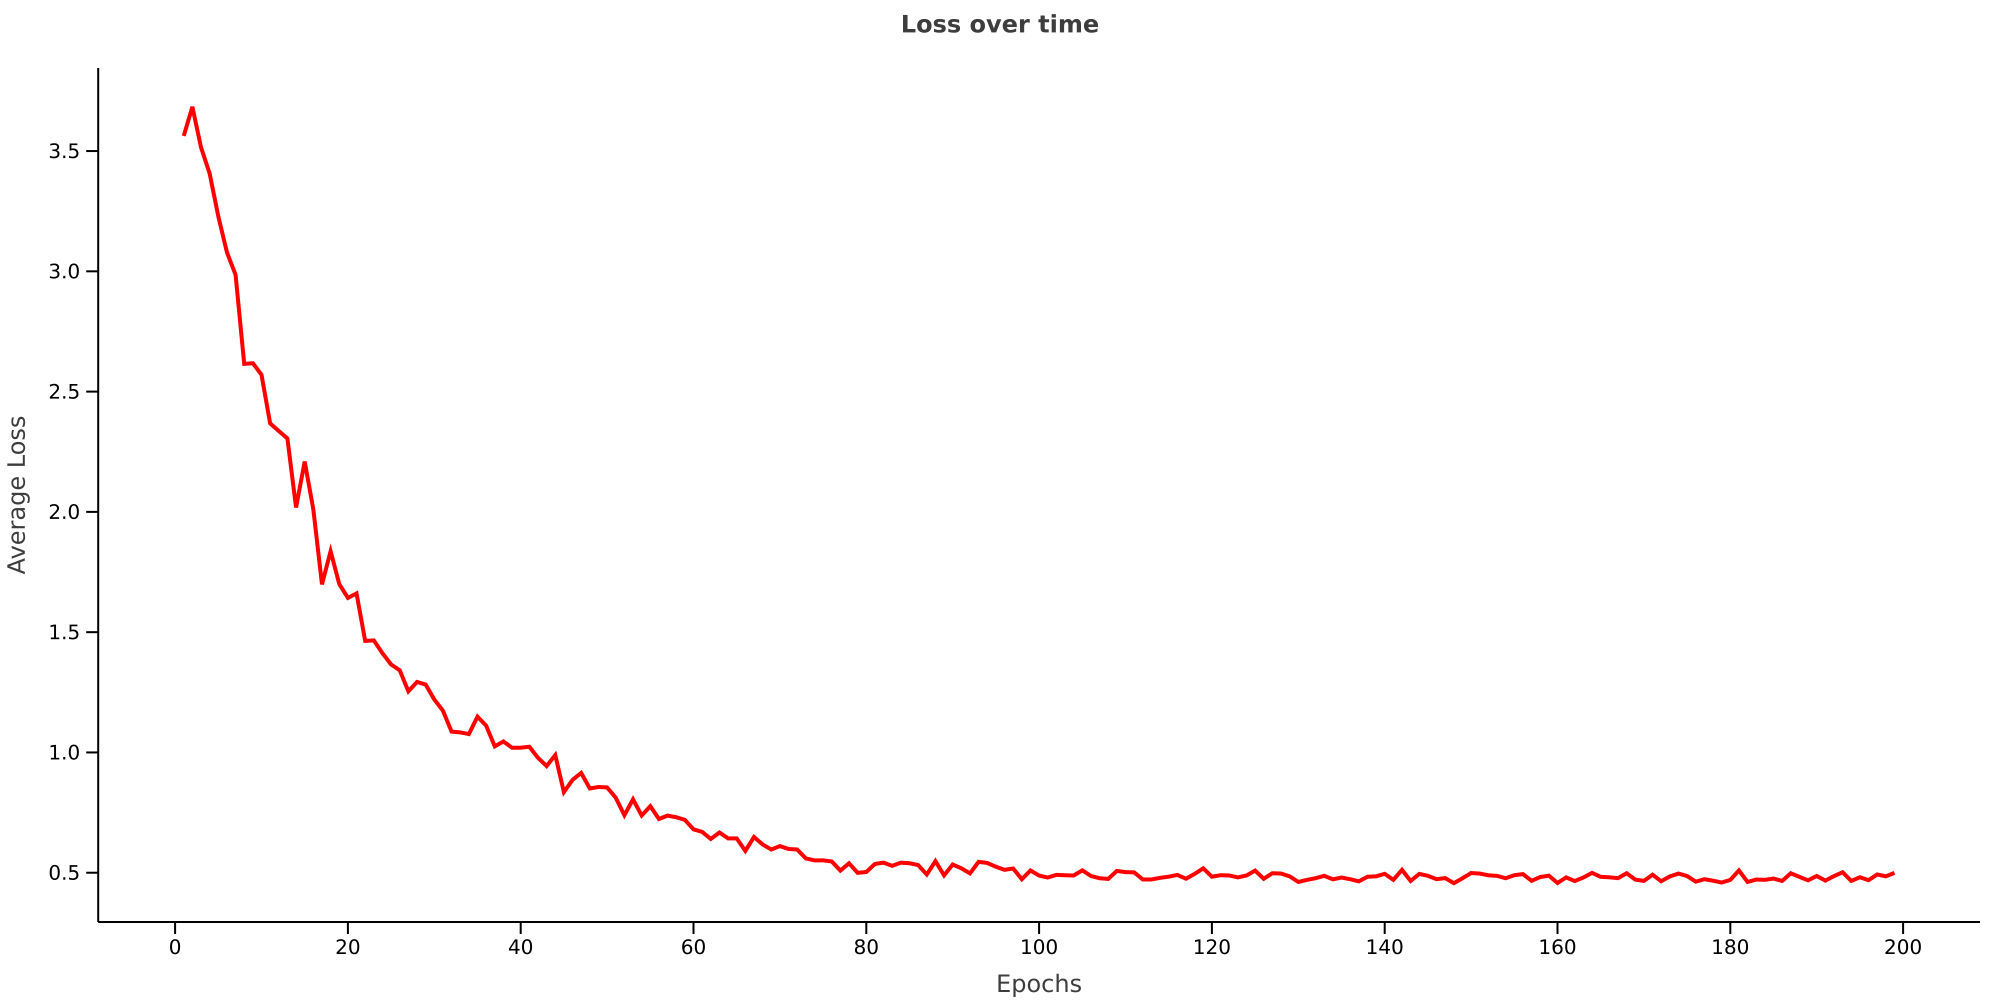
\includegraphics[width=0.80\textwidth]{../figures/training_curve.png}
\caption{Training curve of a single trajectory of gradient descent in the parameter space.}
\label{fig:training_curve}
\end{figure}

\section{Conclusion}

In this chapter we have visited some interesting ideas for validating intelligent systems from the perspective of software engineering and machine learning. We have seen a curious resemblance between some new and old ideas in adversarial learning and fuzz testing. We have proposed a framework for evaluating differentiable programs in a low-cost, data-driven manner and suggest some intriguing directions for future research.

\begin{figure}
\centering
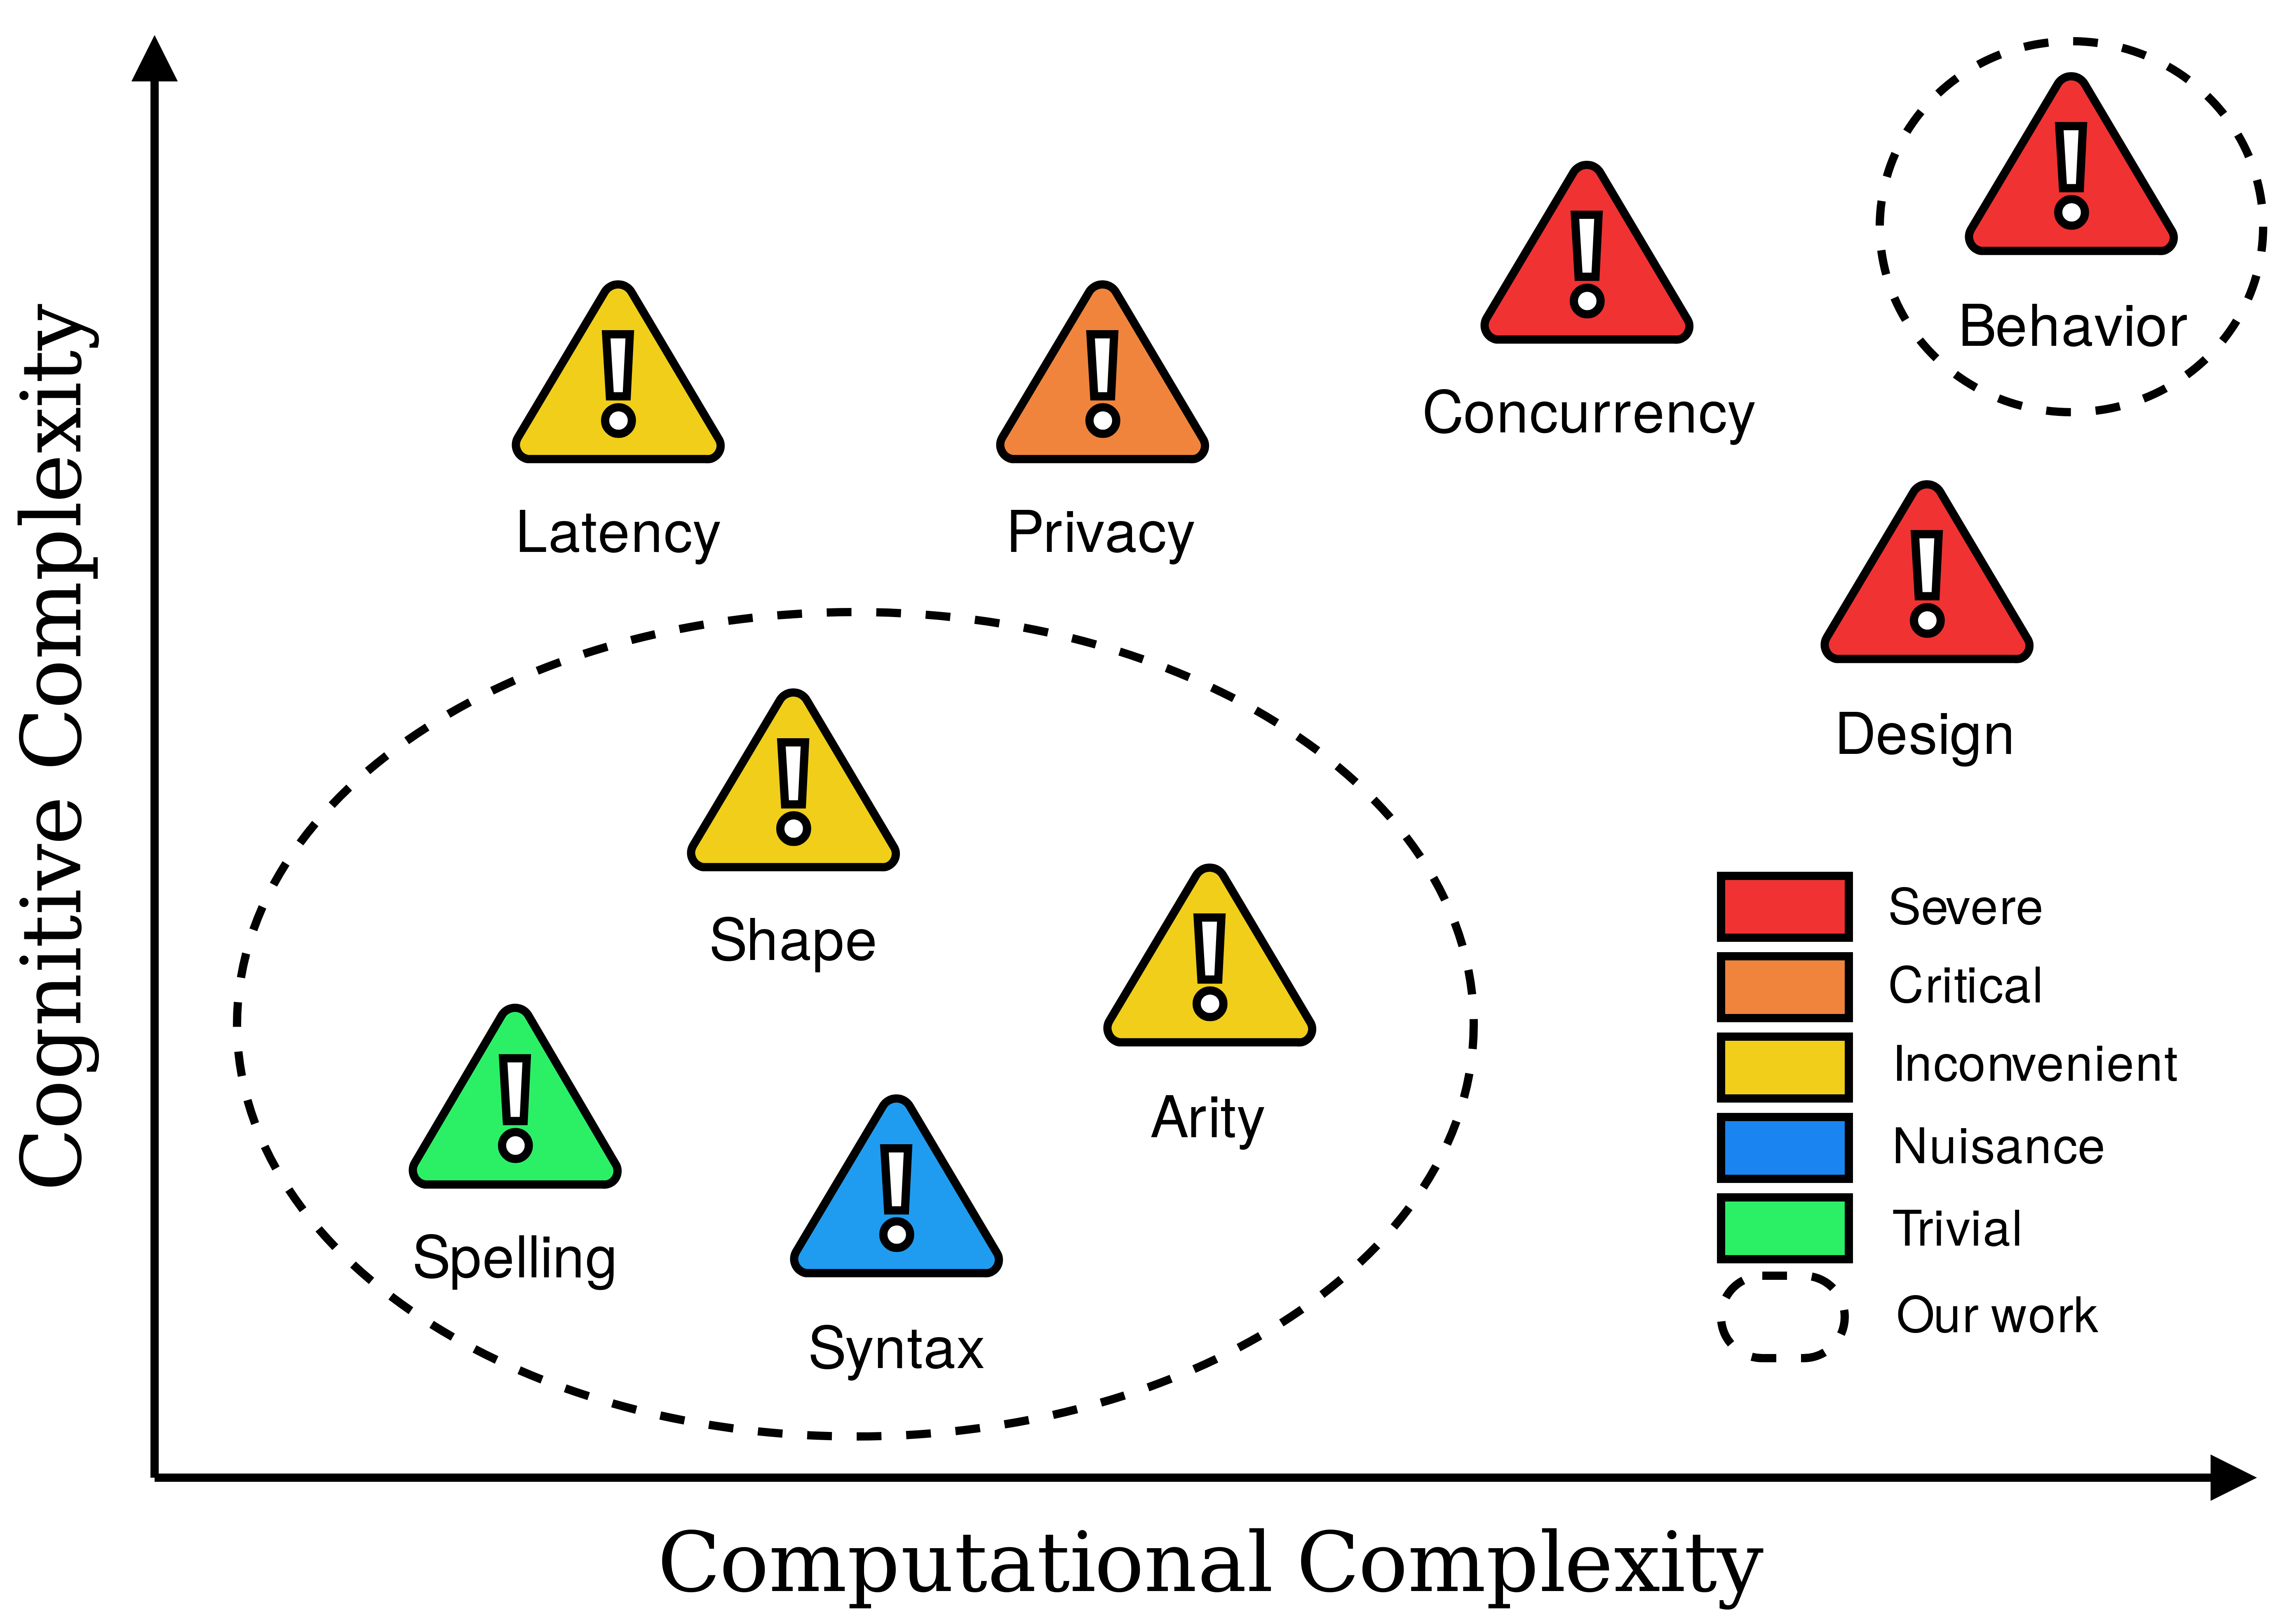
\includegraphics[width=0.60\textwidth]{../figures/verification_complexity.png}
\caption{Complexity of detecting various types of programming errors.}
\label{fig:verification_complexity}
\end{figure}

Type systems, compilers and fuzzers are all part of a broader class of validation and verification tools. The goal of these tools is to provide feedback as early as possible. Some errors (e.g. syntactical errors), are minor nuisances and can be quickly detected with a good incremental parser (\autoref{subsec:the-parser}). Others, as shown in~\autoref{fig:verification_complexity}, are more complex but can be detected by spending computation. We argue this computational cost is often justified as undetected bugs can have catastrophic consequences. Spending computation frees up valuable cognitive resources better spent on more challenging tasks downstream. Studies have shown bugs detected early in development are more likely to be fixed~\citep{distefano2019scaling} -- saving minutes in development could save lives during operation.

Learning capabilities will play a crucial role in autonomous systems. As today's engineers begin to incorporate learning in tomorrow's safety-critical robotic systems, we believe the increased assurance provided by intelligent validation and verification tools will be indispensable for the widespread deployment of these complex adaptive cyberphysical systems.

\chapter{Tools for reproducible robotics}\label{ch:ducker}

\setlength{\epigraphwidth}{0.70\textwidth}
\epigraph{``An article about computational science in a scientific publication is not the scholarship itself, it is merely advertising of the scholarship. The actual scholarship is the complete software development environment and the complete set of instructions which generated the figures.''}{\begin{flushright}--\citet{buckheit1995wavelab}, \href{https://statweb.stanford.edu/~wavelab/Wavelab_850/wavelab.pdf}{\textit{WaveLab and Reproducible Research}}\end{flushright}}

In this chapter, we discuss the challenge of software reproducibility and how best practices in software engineering such as continuous integration and containerization tools can help researchers mitigate the variability associated with building and maintaining robotics software. Broadly, our work attempts to isolate sources of computational variability, and does not consider notions of statistical variability arising from aleatoric or epistemic risk. However, minimizing the computational variability (which often impedes experimental reproducibility) is a key step in enabling researchers to more rapidly identify and diagnose these more elusive variables in robotics and machine learning.

In order to address the issue of software reproducibility, we assembled a set of tools and development workflows representing best practices in software engineering. These tools are primarily based on containerization, a widely adopted virtualization technology in the software industry. To lower the barrier of entry for new contributors and minimize variability across hardware platforms, we developed a state-of-the-art container infrastructure based on Docker~\citep{merkel2014docker}, one popular container engine. Docker allows users to set up versioned deployment artifacts which effectively freeze an entire filesystem, and manage resource constraints via a sandboxed runtime environment.

The contents of this chapter are organized as follows. In \autoref{sec:dependency-management} we introduce the problem of dependency resolution and the challenge of building reproducible software artifacts. In \autoref{sec:os-and-virtualization}, we describe a broad solution to this problem, software virtualization. Next, in \autoref{sec:containerization}, we discuss a lightweight approach to virtualization, known as containerization. In \autoref{sec:docker-intro}, we take a guided tour through one container implementation, called Docker. Finally, in \autoref{sec:ros-docker}, we present DuckieOS, a Dockerized environment for building reproducible robotics applications for research and pedagogical use.

\section{Dependency management}\label{sec:dependency-management}

One common source of variability in software development are software dependencies. For many years, developers struggled with dependency management before it was discovered the dependency resolution problem was NP-complete~\citep{abate2012dependency}. If we assume no two versions of the same dependency can be installed simultaneously, then for a given set of software packages which must be installed, and dependencies required to install them, determining the most recent consistent version of the dependencies is as hard as the hardest problems in NP. Informally, this problem is known as \textit{dependency hell} and becomes increasingly problematic as software projects grow and introduce new dependencies.

Dependency hell does not just arise inside individual software projects, but across projects and development environments. Hundreds of package managers have been developed for various operating systems, programming languages, and development frameworks. Ubuntu has the \href{https://help.ubuntu.com/lts/serverguide/apt.html}{Advanced Package Tool} (\inline{apt}), macOS has \href{https://brew.sh/}{Homebrew} (\inline{brew}), Windows has \href{https://chocolatey.org/}{Chocolatey} (\inline{choco}). Most programming language ecosystems have their own bespoke package managers; \href{https://conan.io/}{Conan} for C/C++, \href{https://maven.apache.org}{Maven} for Java, and \href{https://www.haskell.org/cabal/}{Cabal} for Haskell. Python has developed many overlapping solutions for package management, including \href{https://pypi.org/project/pip/}{pip}, \href{https://www.anaconda.com/}{Anaconda}, \href{https://github.com/pyenv/pyenv}{PyEnv}, \href{https://virtualenv.pypa.io/}{Virtualenv}, and others. Some of these install system-wide packages, and others provide command line environments. Over the lifetime of a computer system, as packages are installed and partially removed it becomes difficult to keep track of changes and their side effects.

The problem basically stems from the requirement that no two versions of the same dependency can be installed simultaneously. In addition, software installers tend to spray files across the file system, which can become corrupted and are difficult to completely remove should the need arise. To address these issues, some notion of ``checkpointing'' is required, so that when new software is installed, any future changes can be traced and reverted. Hardware backups would do the job, but are cumbersome to manage and are unsuitable for development purposes. Rather, it would be convenient to have a tool which allowed applications to create a private file system, install their dependencies, and avoid contaminating the host OS.

\section{Operating systems and virtualization}\label{sec:os-and-virtualization}

With the growth of developer operations (devops) a number of solutions emerged for building and running generic software artifacts. Most primitive of these are emulators, which completely simulate a foreign processor architecture, and thereby any software which runs ontop of it. Another solution are virtual machines (VMs), a kind of isolated runtime environment which use a \textit{hypervisor} to mediate access to hardware, but usually run on bare metal. The downside of both methods is their efficiency. Virtual machines contain full-fledged operating systems and are therefor cumbersome to run and debug. This is particularly unnecessary for building and running a small application on a foreign OS. Emulators run significantly more slowly than native machine code depending on the host and target architectures.

In 2006, Linux introduced several new kernel features for controlling groups of processes, under the aegis of \textbf{cgroups}~\citep{menage2007adding}. Collectively, these features support a form of lightweight virtualization, featuring many of the benefits of virtual machines (VMs) such as resource control and namespace isolation, without the computational overhead associated with full virtualization. These features paved the way for a set of tools that are today known as containers. Unlike VMs, containers share a common kernel, but remain isolated from their host OS and sibling containers. Where VMs often require server-class hardware to run smoothly, containers are suitable for a much broader class of mobile and embedded platforms due to their light resource footprint.

\begin{figure}
    \centering
    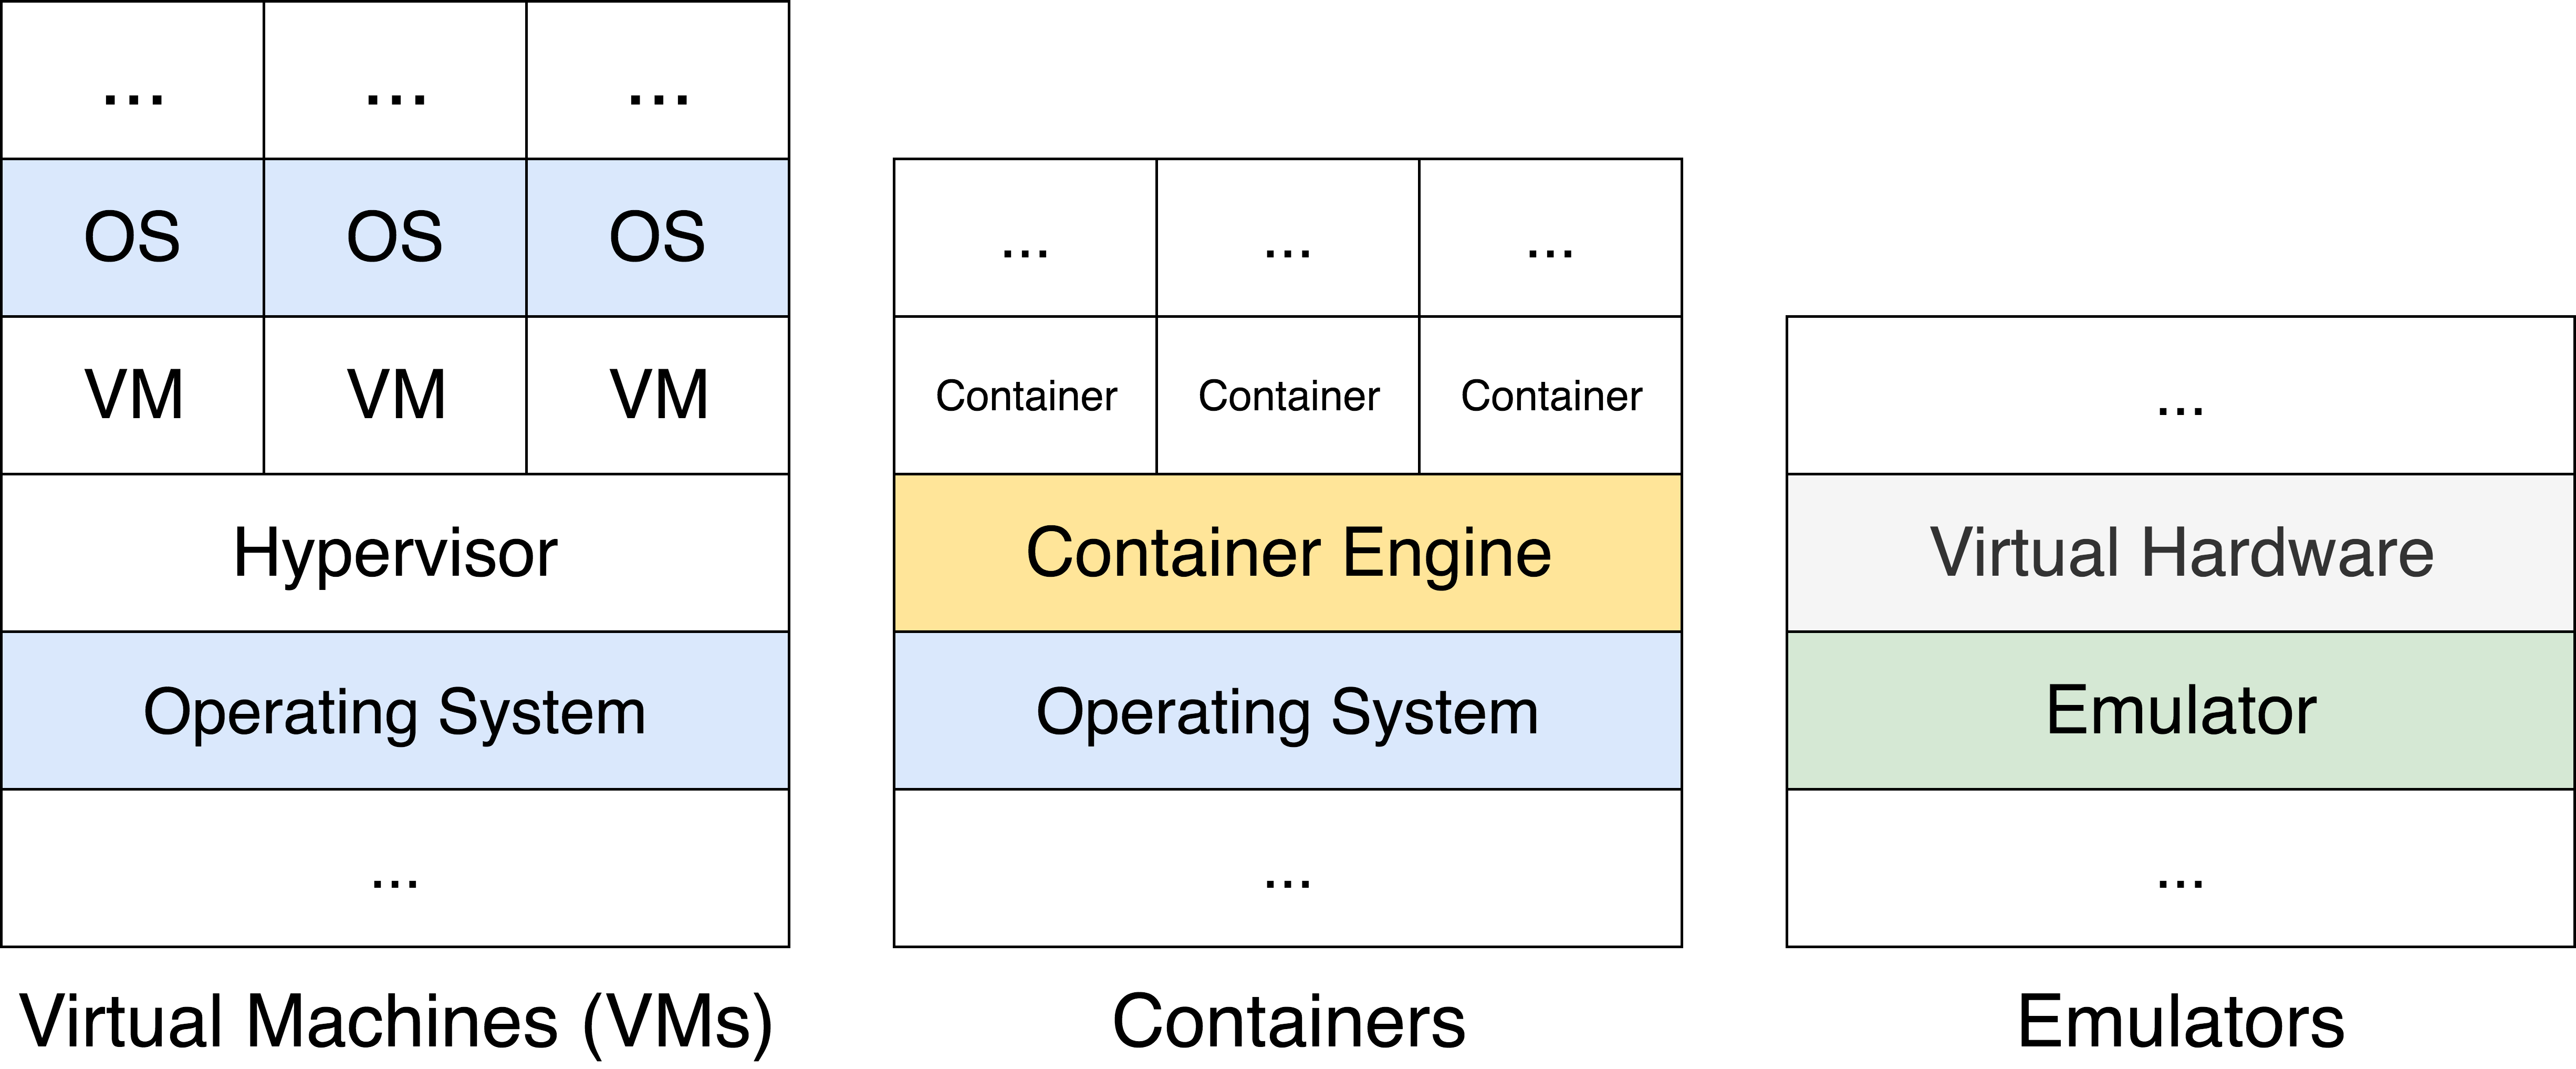
\includegraphics[width=0.70\textwidth]{../figures/vms_containers_emulators.png}
    \caption{Full virtualization is a very resource-hungry process. Containerization is cheaper, as it shares a kernel with the host OS. Emulation lets us emulate hardware as software. Any of these methods can be used in conjunction with any other.\vspace{-10pt}}
    \label{fig:vms_containers_emulators}
\end{figure}

\section{Containerization}\label{sec:containerization}

One of the challenges of distributed software development across heterogeneous platforms is the problem of variability. With today's increasing pace of software development comes the added burden of software maintenance. As hardware and software stacks evolve, source code must periodically be updated to build and run correctly. Maintaining a stable and well-documented codebase can be a considerable challenge, especially in an academic setting where contributors are frequently joining and leaving a project. Together, these challenges present significant obstacles to experimental reproducibility and scientific collaboration.

\begin{figure}[ht]
    \centering
    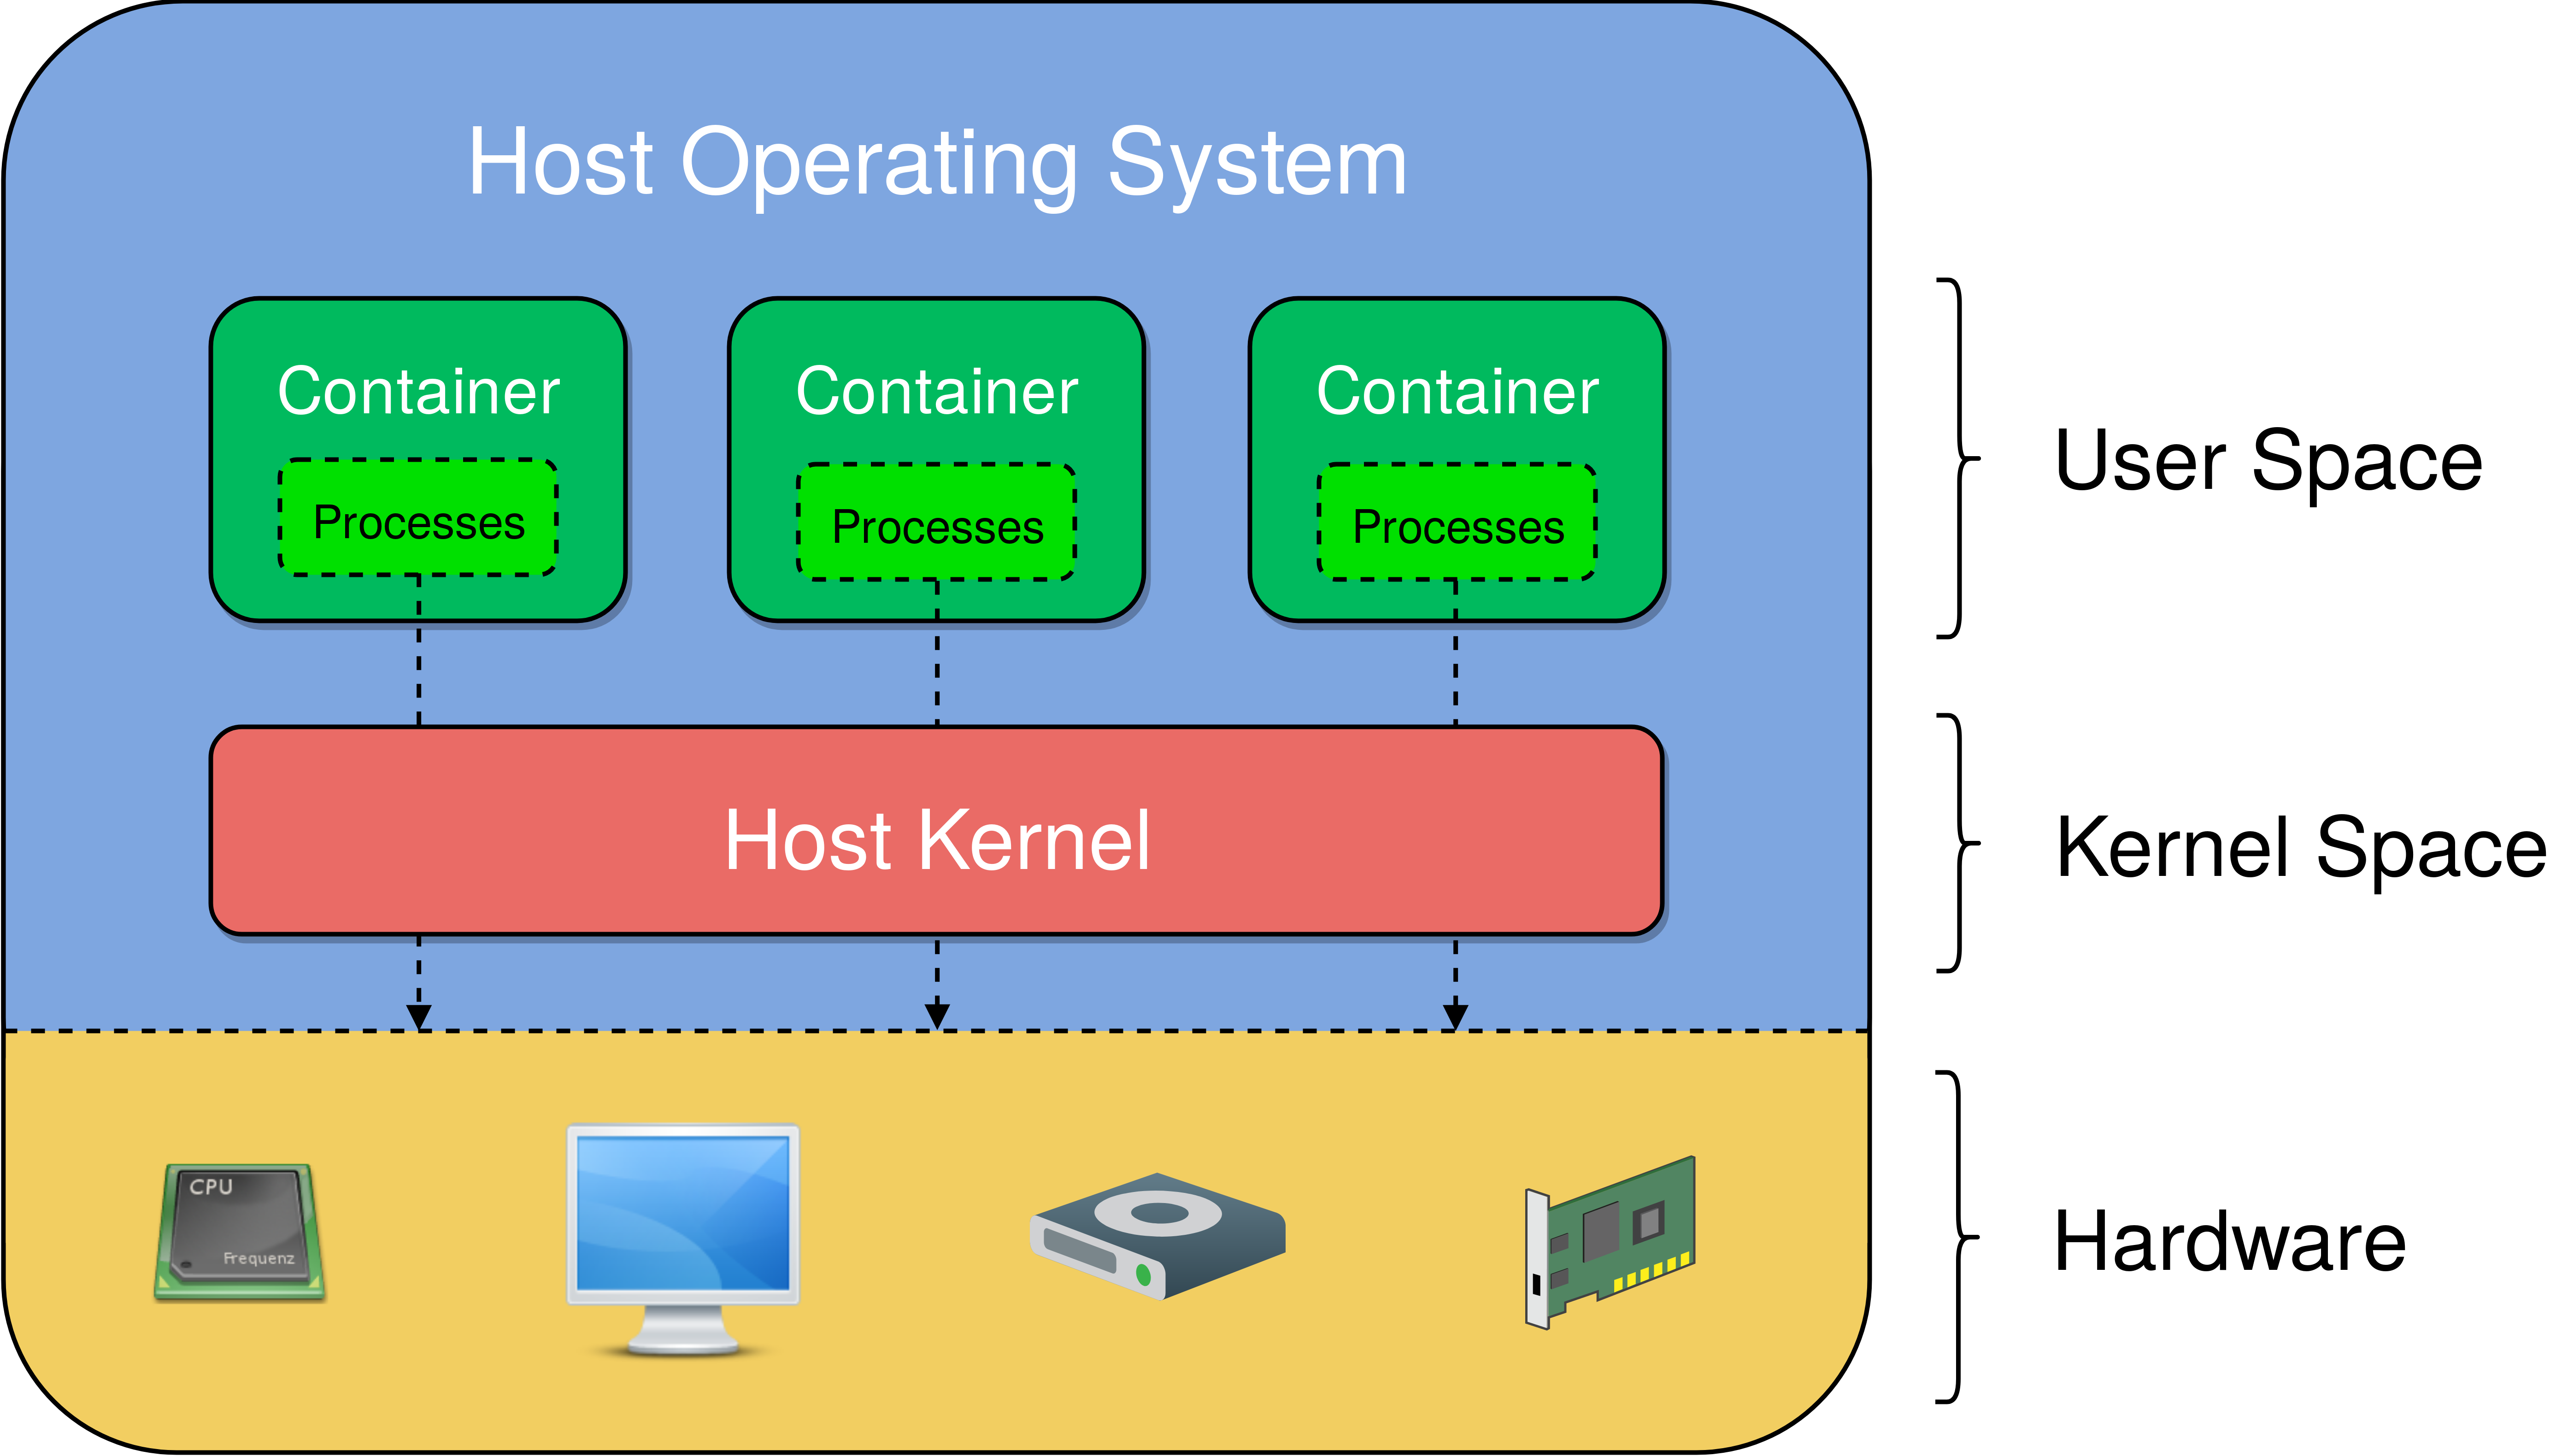
\includegraphics[width=0.65\textwidth]{../figures/user_kernel_hardware.png}
    \caption{Containers live in user space. By default they are sandboxed from the host OS and sibling containers, but unlike VMs, share a common kernel with each other and the host OS. All system calls are passed through host kernel.}
    \label{fig:user_kernel_hardware}
\end{figure}

Docker containers are sandboxed runtime environments that are portable, reproducible and version-controlled. Each environment fully contains its dependencies, but remains isolated from the host OS and file system. Docker provides a mechanism to control the resources each container is permitted to access, and provisions a separate Linux namespace for each container, effectively isolating the network, users, and file system mounts from the host OS. Unlike virtual machines, container-based virtualization tools like Docker are suitable for portable SBCs and can run with close to zero overhead compared to native Linux processes. A single Raspberry Pi is capable of simultaneously running hundreds of containers with no noticeable degradation in performance.\hspace{-.08em}\footnote{\url{https://blog.docker.com/2015/09/update-raspberry-pi-dockercon-challenge/}}

While containerization considerably simplifies the process of building and deploying applications, it also introduces some additional complexity in the software development lifecycle. Docker, like most container platforms, uses a layered filesystem. This enables Docker to take an existing ``image'' and change it by installing new dependencies or modifying its functionality. Images are typically constructed as a sequence of layers, each of which must periodically be updated. Care is required when designing the development pipeline to ensure that such updates do not silently break a subsequent layer, as we describe in \autoref{sec:retrospective}.

\section{Introduction to Docker}\label{sec:docker-intro}

Suppose there is a program which is known to run on some computer. It would be nice to give another computer -- any computer with an internet connection -- a short string of ASCII characters, press \keys{\return}, and return to see that same program running. Never mind where the program was built or what software happened to be running at the time. This may seem trivial, but is a monumental software engineering problem. Various package managers have attempted to solve this, but even when they work as intended, only support natively compiled binaries on operating systems with the same package manager.

Docker\footnote{The following tutorial uses Docker, but the workflow described is similar to most container platforms.} is a tool for portable, reproducible computing. With Docker, users can run any Linux program on almost any networked computing device on the planet, regardless of the underlying operating system or hardware architecture. All of the environment preparation, installation and configuration steps can be automated from start to finish. Depending on how much network bandwidth is available, it might take some time, but users will never need to intervene in the installation process.

To install Docker itself, execute the following command on a POSIX-compliant shell of any \href{https://docs.docker.com/install/#supported-platforms}{Docker-supported platform}:

\begin{pclisting}
~$ curl -sSL https://get.docker.com/ | sh
\end{pclisting}
%
A Docker \textit{image} is basically a filesystem snapshot -- a single file that contains everything needed to run a certain Docker container. Docker images are hosted in \textit{registries}, similar to Git repositories or VCS servers. The following command will fetch a Docker image, e.g. \inline{daphne/duck} from the default \hyperref[subsec:docker_hub]{Docker Hub} repository:

\begin{pclisting}
~$ docker pull daphne/duck
\end{pclisting}
%
Every Docker image has an image ID, a name and a tag:

\begin{pclisting}
~$ docker images
REPOSITORY      TAG        IMAGE ID         CREATED       SIZE
daphne/duck     latest     ea2f90g8de9e     1 day ago     869MB
\end{pclisting}
%
To run a Docker container\footnote{When a Docker image is running, it is referred to as a \textit{container}.}, use the following command:

\begin{pclisting}
~$ docker run daphne/duck
\end{pclisting}
%
The following command will verify the container is indeed running:

\begin{pclisting}
~$ docker ps
CONTAINER ID     IMAGE           ...     NAMES
52994ef22481     daphne/duck     ...     happy_hamster
\end{pclisting}
%
Note how Daphne's duck container has an alphanumeric container ID, a base image, and a memorable name, \inline{happy\_hamster}. This name is an alias for the container ID, which can be used interchangeably to refer to the container.

Docker images can be created two different ways. First, in \autoref{subsec:creating-an-image-snapshot}, we will see how to create a Docker image by taking a snapshot from a running container, then in \autoref{subsec:writing-an-image-recipe}, how to create a new Docker container using a special kind of recipe, called a \href{https://docs.docker.com/engine/reference/builder/}{\inline{Dockerfile}}.

\subsection{Creating an image snapshot}\label{subsec:creating-an-image-snapshot}

When a Docker container writes to its own filesystem, those changes are not persisted unless committed to a new image. For example, start a container with an interactive shell:

\begin{pclisting}
~$ docker run -it daphne/duck /bin/bash
root@295fd7879184:/#
\end{pclisting}
%
Note the container ID: \inline{295fd7879184}. If we write to disk and leave the container,

\begin{pclisting}
root@295fd7879184:/# touch new_file && ls -l
total 0
-rw-r--r-- 1 root root 0 May 21 20:52 new_file
root@295fd7879184:/# exit
\end{pclisting}
%
\inline{new\_file} will not be persisted. If we re-run the same command again:

\begin{pclisting}
~$ docker run -it daphne/duck /bin/bash
root@18f13bb4571a:/# ls
root@18f13bb4571a:/# touch new_file1 && ls -l
total 0
-rw-r--r-- 1 root root 0 May 21 21:32 new_file1
\end{pclisting}
%
It seems like \inline{new\_file} has disappeared! Notice how the container ID (\inline{18f13bb4571a}) is now different. This is because the command \inline{docker run daphne/duck} created a new container from the base image \inline{daphne/duck}, rather than restarting the previous container. To see all containers on a Docker host, run the following command:

\begin{pclisting}
~$ docker container ls -a
CONTAINER ID      IMAGE            STATUS             NAMES
295fd7879184      daphne/duck      Exited (130)       merry_manatee
18f13bb4571a      daphne/duck      Up 5 minutes       shady_giraffe
52994ef22481      daphne/duck      Up 10 minutes      happy_hamster
\end{pclisting}
%
It appears \inline{295fd7879184} a.k.a. \inline{merry\_manatee} survived, but it is no longer running. Whenever a container's main process (recall we ran \inline{merry\_manatee} with \inline{/bin/bash}) finishes, the container will stop, but it will not cease to exist. In fact, we can resume the stopped container right where it left off:
%
\begin{pclisting}
~$ docker start -a merry_manatee
root@295fd7879184:/# ls -l
total 0
-rw-r--r-- 1 root root 0 May 21 20:52 new_file
\end{pclisting}
%
Nothing was lost! To verify this, we can check which other containers are running:

\begin{pclisting}
~$ docker ps
CONTAINER ID       IMAGE             ...       NAMES
295fd7879184       daphne/duck       ...       merry_manatee
18f13bb4571a       daphne/duck       ...       shady_giraffe
52994ef22481       daphne/duck       ...       happy_hamster
\end{pclisting}
%
Now suppose we would like to share the container \inline{shady\_giraffe} with someone else. To do so, we must first snapshot the running container, or commit it to a new image with a name and a tag. This will create a checkpoint that we may later restore:

\begin{pclisting}
~$ docker commit -m "forking daphne/duck" shady_giraffe user/duck:v2
\end{pclisting}
%
To refer to the container, we can either use \inline{18f13bb4571a} or the designated name (i.e. \inline{shady\_giraffe}). This image repository will be called \inline{user/duck}, and has an optional version identifier, \inline{:v2}, which can be pushed to the \hyperref[subsec:docker_hub]{Docker Hub} registry:

\begin{pclisting}
~$ docker push user/duck:v2
~$ docker images
REPOSITORY    TAG        IMAGE ID         CREATED          SIZE
daphne/duck   latest     ea2f90g8de9e     1 day ago        869MB
user/duck     v2         d78be5cf073e     2 seconds ago    869MB
~$ docker pull user/duck:v2
~$ docker run user/duck ls -l
total 0
-rw-r--r-- 1 root root 0 May 21 21:32 new_file1
\end{pclisting}
%
This is a convenient way to share an image with colleagues and collaborators. Anyone with access to the repository can pull this image and continue where we left off, or create another image based on top.

\subsection{Writing an image recipe}\label{subsec:writing-an-image-recipe}

The second way to create a Docker image is to write a recipe, called a \inline{Dockerfile}. A \inline{Dockerfile} is a text file that specifies the commands required to create a Docker image, typically by modifying an existing container image using a scripting interface. They also have special \href{https://docs.docker.com/engine/reference/builder/}{keywords} (which are conventionally \inline{CAPITALIZED}), like \href{https://docs.docker.com/engine/reference/builder/#from}{\inline{FROM}}, \href{https://docs.docker.com/engine/reference/builder/#from}{\inline{RUN}}, \href{https://docs.docker.com/engine/reference/builder/#entrypoint}{\inline{ENTRYPOINT}} and so on. For example, create a file called \inline{Dockerfile} with the following content:

\begin{dockerlisting}
FROM daphne/duck      # Defines the base image
RUN touch new_file1   # new_file1 will be part of our snapshot
CMD ls -l             # Default command run when container is started
\end{dockerlisting}
%
Now, to build the image, we can simply run:

\begin{pclisting}
~$ docker build -t user/duck:v3 (*\hl{.}*)
\end{pclisting}
%
The \inline{.} indicates the current directory, which should be the same one containing our \inline{Dockerfile}. This command should produce something like the following output:

\begin{pclisting}
Sending build context to Docker daemon  2.048kB
Step 1/3 : FROM daphne/duck
--- ea2f90g8de9e
Step 2/3 : RUN touch new_file1
--- e3b75gt9zyc4
Step 3/3 : CMD ls -l
--- Running in 14f834yud59
Removing intermediate container 14f834yud59
--- 05a3bd381fc2
Successfully built 05a3bd381fc2
Successfully tagged user/duck:v3
\end{pclisting}
%
The command, \inline{docker images} should display an image called \inline{user/duck:v3}:

\begin{pclisting}
~$ docker images
REPOSITORY    TAG        IMAGE ID         CREATED          SIZE
daphne/duck   latest     ea2f90g8de9e     1 day ago        869MB
user/duck     v2         d78be5cf073e     5 minutes ago    869MB
user/duck     v3         05a3bd381fc2     2 seconds ago    869MB
\end{pclisting}
%
This procedure is identical to the snapshot technique performed in \autoref{subsec:creating-an-image-snapshot}, but the result is cleaner. Rather than maintaining a 869 MB image, we can just store the 4 KB text file instead. To run the resulting image, we can simply use the same command as before:

\begin{pclisting}
~$ docker run -it user/duck:v3
total 0
-rw-r--r-- 1 root root 0 May 21 21:35 new_file1
\end{pclisting}
%
Notice that as soon as we run the container, Docker will execute the \inline{ls -l} command as specified by the \inline{Dockerfile}, revealing that \inline{new\_file1} was indeed stored in the image. However, this default command can be overridden by supplying a custom command:

\begin{pclisting}
~$ docker run -it user/duck:v3 [custom_command]
\end{pclisting}
%
\subsection{Layer Caching}

\href{https://docs.docker.com/storage/storagedriver/#images-and-layers}{Layers} are an important concept to understand when working with Docker. One way to think of a layer is like a Git commit -- a set of changes to a previous image or layer, uniquely identified by a hash code. In a \inline{Dockerfile}, layers begin with a \href{https://docs.docker.com/engine/reference/builder/#from}{keyword}.

\begin{dockerlisting}
FROM daphne/duck
RUN touch new_file1                            # Defines a new layer
RUN mkdir config && mv new_file1 config        # Layers can chain commands
RUN apt-get update && apt-get install -y wget  # Install a dependency
RUN wget https://get.your.app/install.sh       # Download a script
RUN chmod +x install.sh && ./install.sh        # Run the script
\end{dockerlisting}
%
To build this image, we can run the following command:

\begin{pclisting}
~$ docker build -t user/duck:v4 .
Sending build context to Docker daemon  2.048kB
Step 1/6 : FROM daphne/duck
---> cd6d8154f1e1
...
Removing intermediate container 8fb56ef38bc8
---> 3358ca1b8649
Step 5/6 : RUN wget https://get.your.app/install.sh
---> Running in e8284ff4ec8b
...
2018-10-30 06:47:57 (89.9 MB/s) - 'install.sh' saved [13847/13847]
Removing intermediate container e8284ff4ec8b
---> 24a22dc2900a
Step 6/6 : RUN chmod +x install.sh && ./install.sh
---> Running in 9526651fa492
# Executing install script, commit: 36b78b2
...
Removing intermediate container 9526651fa492
---> a8be23fea573
Successfully built a8be23fea573
Successfully tagged user/duck:v4
\end{pclisting}
%
Layers are conveniently cached by the \href{https://docs.docker.com/engine/reference/commandline/dockerd/}{Docker daemon}. Should we need to run the same command twice, Docker will use the cache instead of rebuilding the entire image:

\begin{pclisting}
Sending build context to Docker daemon  2.048kB
Step 1/6 : FROM daphne/duck
---> cd6d8154f1e1
Step 2/6 : RUN touch new_file1
---> Using cache
---> 0473154b2004
...
Step 6/6 : RUN chmod +x index.html && ./index.html
---> Using cache
---> a8be23fea573
Successfully built a8be23fea573
Successfully tagged user/duck:v4
\end{pclisting}
%
If we need to make a change to the \inline{Dockerfile}, Docker will only rebuild the image starting from the first modified step. Suppose we were to add a new \inline{RUN} command at the end of our \inline{Dockerfile} and trigger a rebuild like so:

\begin{pclisting}
~$ echo 'RUN echo "Change here!"' >> Dockerfile
~$ docker build -t user/duck:v4 .
Sending build context to Docker daemon  2.048kB
...
Step 6/7 : RUN chmod +x index.html && ./index.html
---> Using cache
---> a8be23fea573
Step 7/7 : RUN echo "Change here!"
---> Running in 80fc5c402304
Change here!
Removing intermediate container 80fc5c402304
---> c1ec64cef9c6
Successfully built c1ec64cef9c6
Successfully tagged user/duck:v4
\end{pclisting}
%
If Docker had to rerun the entire \inline{Dockerfile} from top to bottom each time it was rebuilt, this would be slow and inconvenient. Instead, Docker caches the unmodified steps by default, and only reruns the minimum set of steps necessary to rebuild. This can sometimes introduce unexpected results, especially when the cache is stale. To ignore the cache and force a clean rebuild, use the \inline{-{}-no-cache} flag when building a \inline{Dockerfile}.

What does Docker consider when deciding whether to use the cache? First is the \inline{Dockerfile} itself -- when a step in a \inline{Dockerfile} changes, both it and any subsequent steps will need to be rerun during a build. Docker also checks the \href{https://docs.docker.com/engine/reference/commandline/build/#extended-description}{build context} for changes. When \inline{docker build -t TAG .} is written, the \inline{.} indicates the build context, or path where the build should occur. Often, this path contains build artifacts. For example:

\begin{dockerlisting}
FROM daphne/duck
COPY duck.txt .
RUN cat duck.txt
\end{dockerlisting}
%
Now if we add some message in \inline{duck.txt} and rebuild our image, the file will be copied into the Docker image, and its contents will be printed:

\begin{pclisting}
~$ echo "Make way!" > duck.txt && docker build -t user/duck:v5 .
Sending build context to Docker daemon  3.072kB
Step 1/3 : FROM daphne/duck
---> cd6d8154f1e1
Step 2/3 : COPY duck.txt .
---> e0e03d9e1791
Step 3/3 : RUN cat duck.txt
---> Running in 590c5420ce29
Make way!
Removing intermediate container 590c5420ce29
---> 1633e3e10bef
Successfully built 1633e3e10bef
Successfully tagged user/duck:v5
\end{pclisting}
%
As long as the first three lines of the \inline{Dockerfile} and \inline{duck.txt} are unmodified, these layers will be cached and Docker will not rebuild them. If the contents of the file \inline{duck.txt} are subsequently modified, this will trigger a rebuild to occur. For example, if we append to the file and rebuild, only the last two steps will need to be executed:

\begin{pclisting}
~$ echo "Thank you. Have a nice day!" >> duck.txt
~$ docker build -t user/duck:v5 .
Sending build context to Docker daemon  3.072kB
Step 1/3 : FROM ubuntu
---> cd6d8154f1e1
Step 2/3 : COPY duck.txt .
---> f219efc150a5
Step 3/3 : RUN cat duck.txt
---> Running in 7c6f5f8b73e9
Make way!
Thank you. Have a nice day!
Removing intermediate container 7c6f5f8b73e9
---> e8a1db712aee
Successfully built e8a1db712aee
Successfully tagged user/duck:v5
\end{pclisting}
%
A common mistake when writing \inline{Dockerfile}s is to \inline{COPY} more files than are strictly necessary to perform the following build step. For example, if \inline{COPY . .} is written at the beginning of the \inline{Dockerfile}, whenever any file is changed within the build context, this will trigger a rebuild of all subsequent build steps. In order to maximize cache reusability and minimize rebuild time, users should be as conservative as possible and only \inline{COPY} the minimum set of files necessary to accomplish the following build step.

% Like Git's \inline{.gitignore}, Docker also has a \inline{.dockerignore} file. If we add a line to the \inline{.dockerignore} file, then all paths matching this line in the build context will be ignored. Docker also accepts other patterns like regular expressions and negation.~\footnote{Further details: \url{https://docs.docker.com/engine/reference/builder/#dockerignore-file}}

\subsection{Volume Sharing}\label{subsec:volume_sharing}

There is a second method of depositing data into a container, which does not require baking it into the parent image at compile-time. This method is more appropriate for data which is required at runtime, but non-essential for the build. It takes the following form:

\begin{pclisting}
~$ docker run user/duck:v6 (*\hl{-v HOST\_PATH:TARGET\_PATH}*)
\end{pclisting}
%
Suppose we have a \inline{Dockerfile} which provides a default \inline{CMD} instruction:

\begin{dockerlisting}
FROM daphne/duck
CMD /bin/bash -c "/launch.sh"
\end{dockerlisting}
%
If we built this image and tried to run it, the file \inline{launch.sh} would be missing:

\begin{pclisting}
~$ docker build -t user/duck:v6 && docker run user/duck:v6
bash: /launch.sh: No such file or directory
\end{pclisting}
%
Instead, when running the container, we need to share the file via the Docker CLI:

\begin{pclisting}
~$ echo -e '#!/bin/bash\necho Launching...' >> launch.sh && \
   chmod 775 launch.sh && \
   docker run user/duck:v6 (*\hl{-v launch.sh:/launch.sh}*)
Launching...
\end{pclisting}
%
This way, the local file \inline{launch.sh} will be available to use from within the container at the designated path, \inline{/launch.sh}.

\subsection{Multi-stage builds}

Docker's filesystem is additive, so each layer will only increase the size of the final image. For this reason, it is often necessary to tidy up unneeded files after installation. For example, when installing dependencies on Debian-based images, it is a common practice to run:

\begin{dockerlisting}
RUN apt-get update && apt-get install ... && (*\hl{rm -rf /var/lib/apt/lists/*}*)
\end{dockerlisting}
%
This ensures the package list is not baked into the image (Docker will only checkpoint the layer after each step is complete). Builds can often consume several steps, despite only producing a single artifact. Instead of chaining together several commands and cleaning up changes in a single step, multi-stage builds let us build a series of images inside a \inline{Dockerfile}, and copy resources from one to another, discarding all intermediate build artifacts:

\begin{dockerlisting}
FROM user/duck:v3 as template1

FROM daphne/duck as template2
COPY --from=template1 new_file1 new_file2
FROM donald/duck as template3
COPY --from=template2 new_file2 new_file3
CMD ls -l
\end{dockerlisting}
%
Now we can build and run this image as follows:

\begin{pclisting}
~$ docker build . -t user/duck:v4
Sending build context to Docker daemon  2.048kB
Step 1/6 : FROM user/duck:v3 as template1
--- e3b75ef8ecc4
Step 2/6 : FROM daphne/duck as template2
--- ea2f90g8de9e
Step 3/6 : COPY --from=template1 new_file1 new_file2
---> 72b96668378e
Step 4/6 : FROM donald/duck:v3 as template3
---> e3b75ef8ecc4
Step 5/6 : COPY --from=template2 new_file2 new_file3
---> cb1b84277228
Step 6/6 : CMD ls
---> Running in cb1b84277228
Removing intermediate container cb1b84277228
---> c7dc5dd63e77
Successfully built c7dc5dd63e77
Successfully tagged user/duck:v4
~$ docker run -it user/duck:v4
total 0
-rw-r--r-- 1 root root 0 Jul  8 15:06 new_file3
\end{pclisting}
%
One application of multi-stage builds is compiling a project dependency from its source code. In addition to all the source code, the compilation process could introduce gigabytes of build artifacts and transitive dependencies, just to build a single binary. Multi-stage builds allow us to build the file, and copy it to a fresh layer, unburdened by intermediate files.

\section{ROS and Docker}\label{sec:ros-docker}

\begin{figure}[ht]
    \centering
    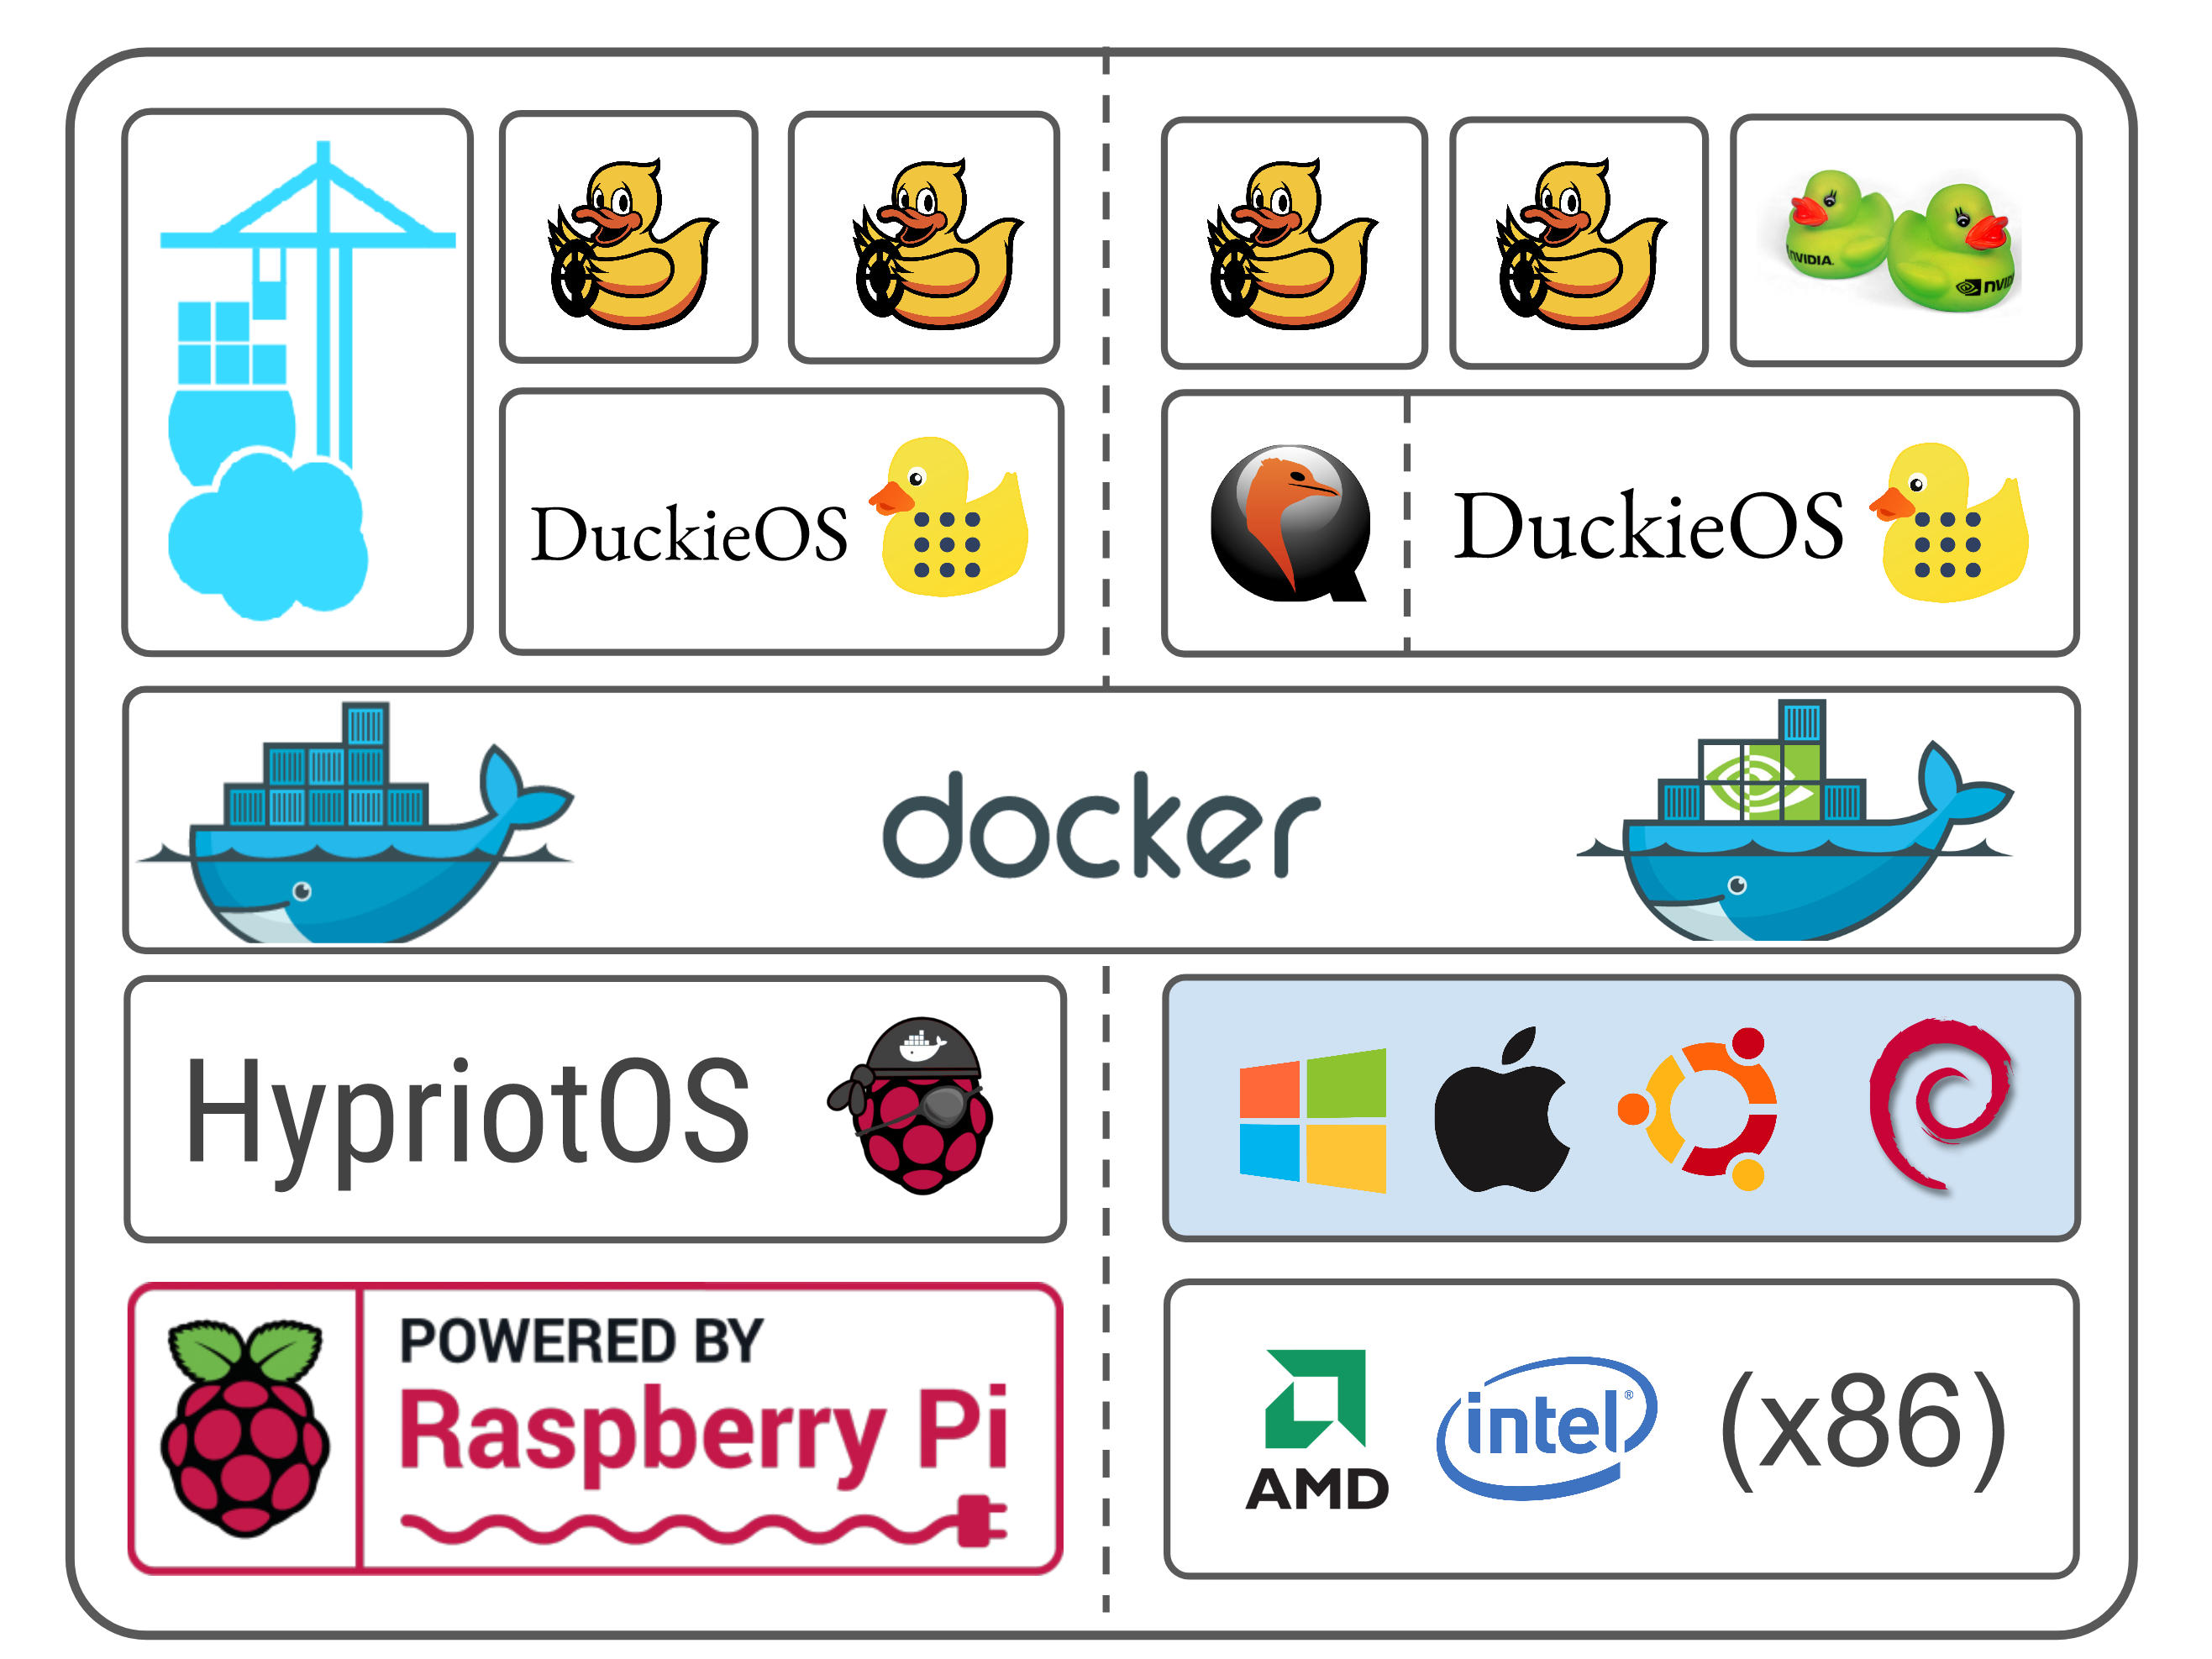
\includegraphics[width=0.48\textwidth]{../figures/docker_stack_1.png}
    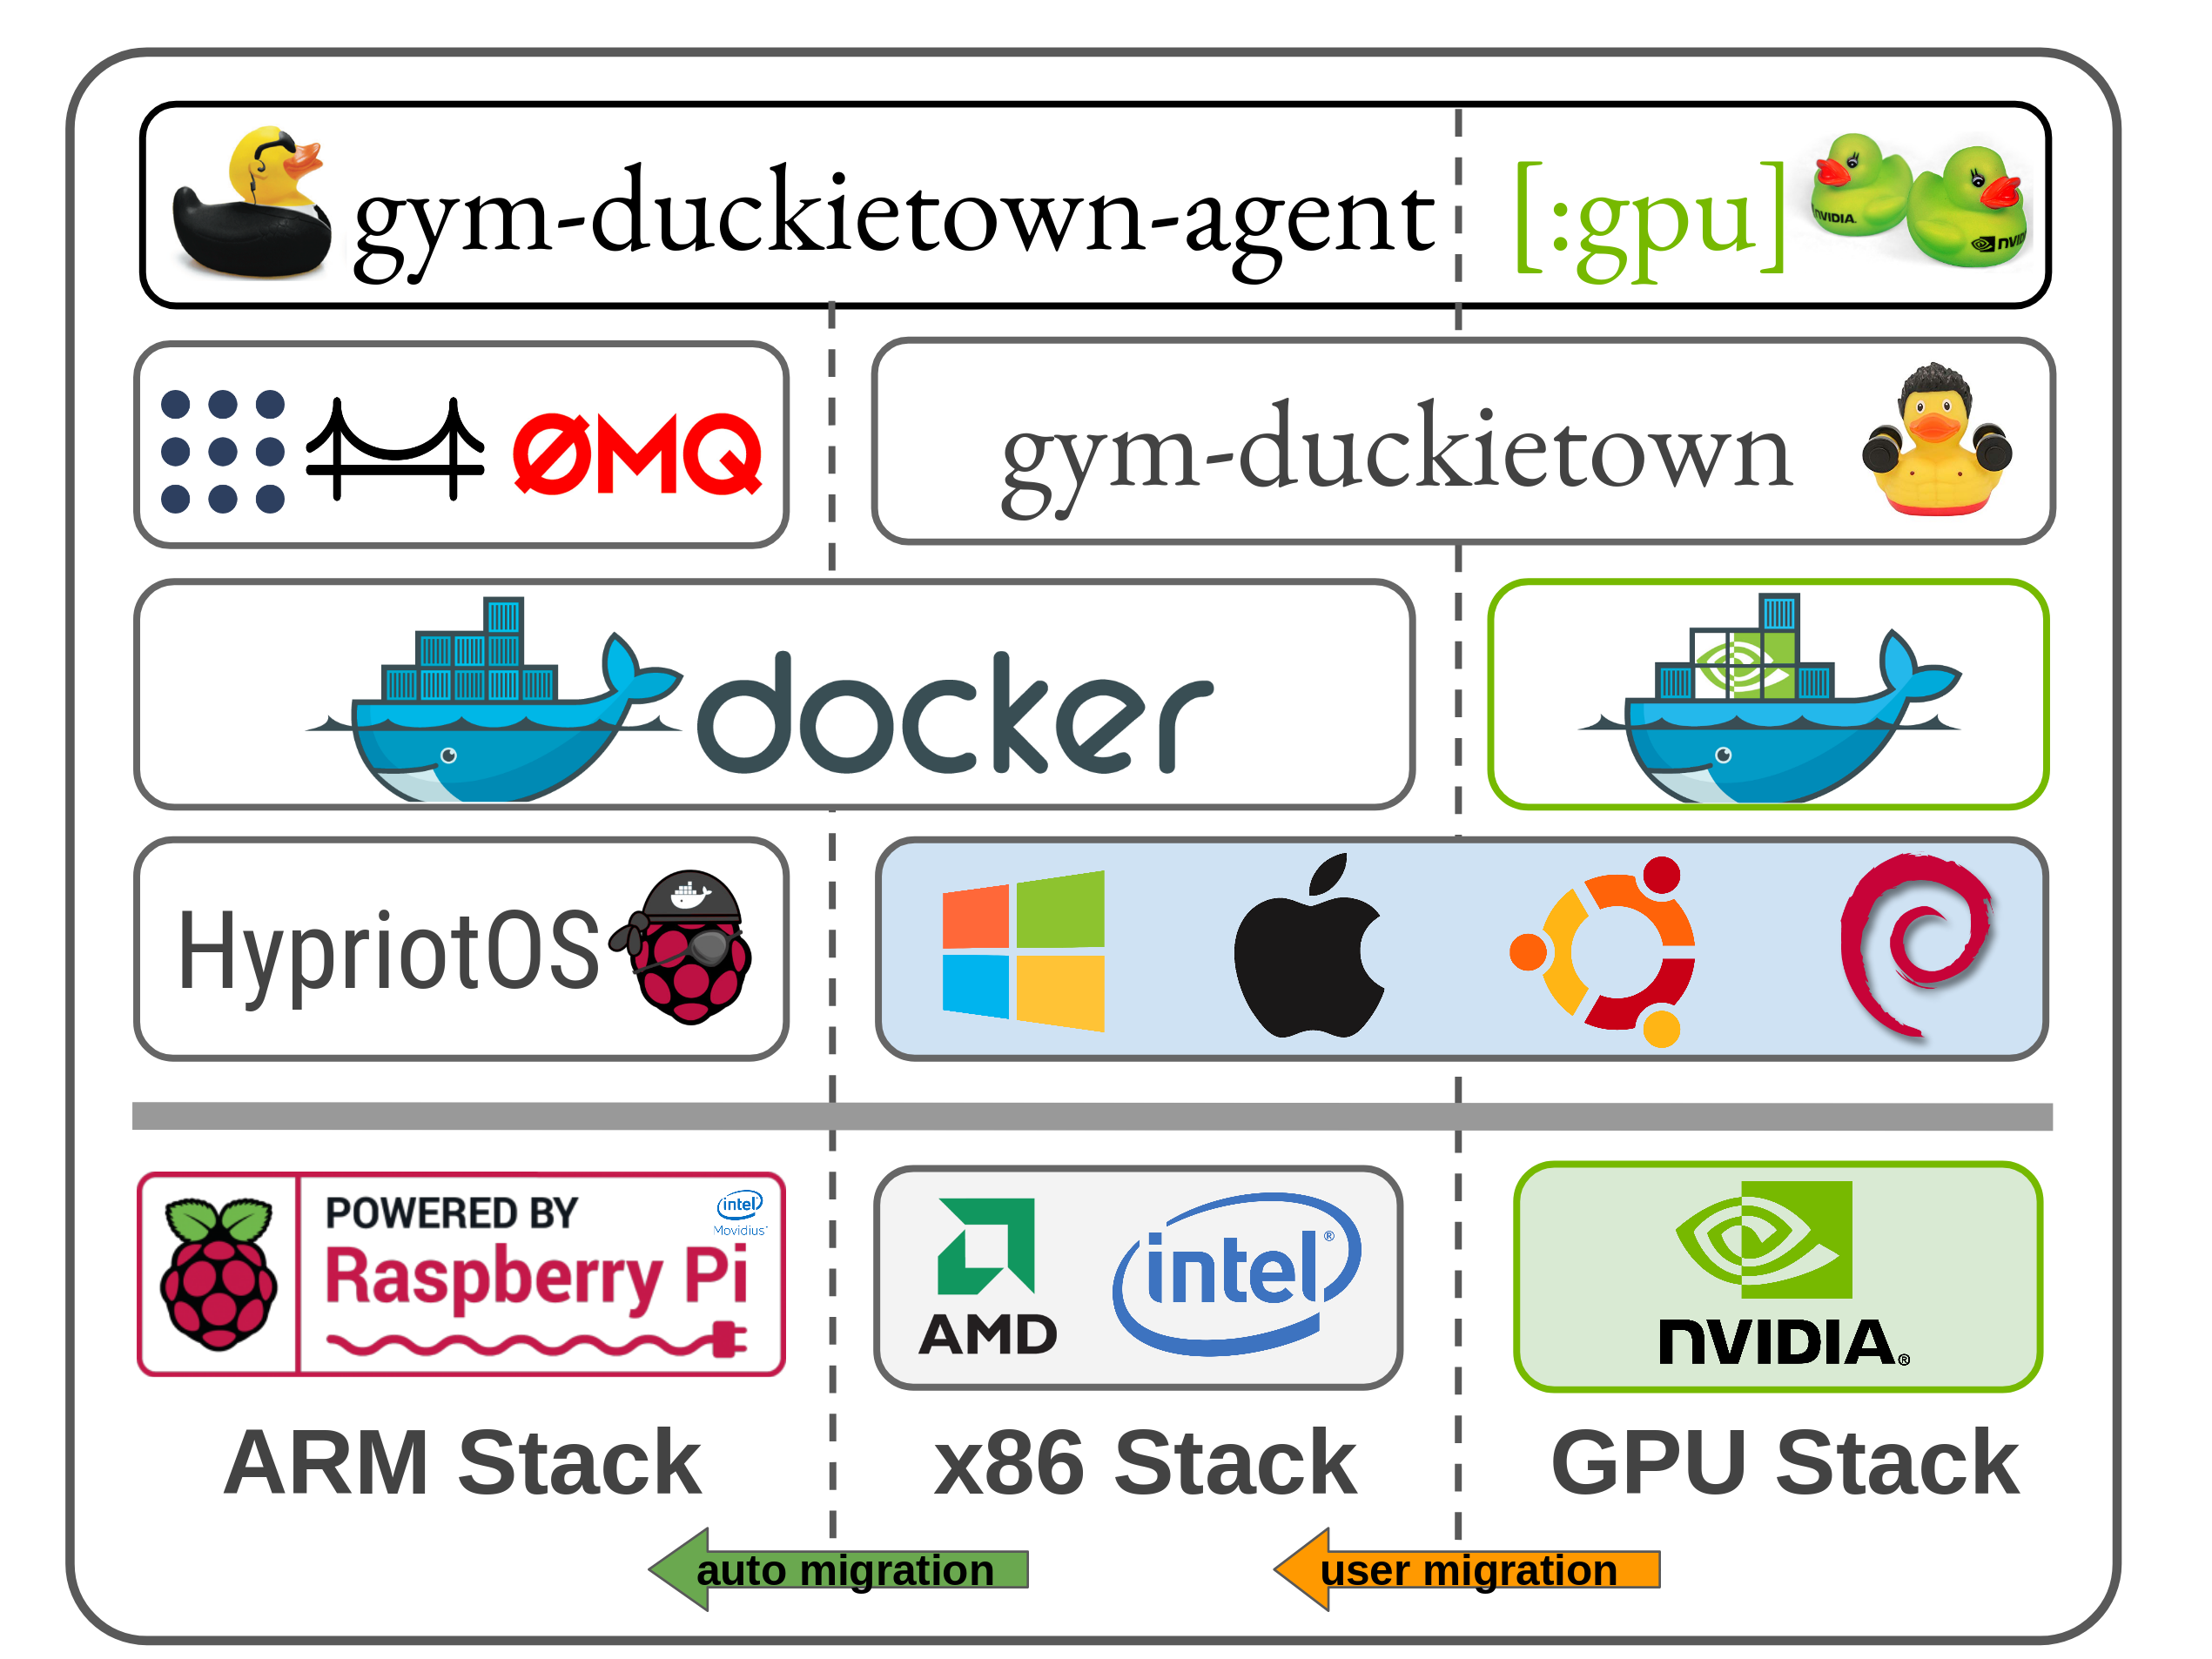
\includegraphics[width=0.48\textwidth]{../figures/docker_stack_2.png}
    \caption{Container infrastructure. \textbf{Left}: The ROS stack targets two primary architectures, x86 and ARM. To simplify the build process, we build ARM artifacts on x86 using \href{https://www.qemu.org}{QEMU}~\citep{bellard2005qemu}. \textbf{Right}: Reinforcement learning stack. Build artifacts are trained on a GPU, and transferred to CPU for evaluation. Deep learning models may be also be run on an ARM device using an \href{https://software.intel.com/en-us/neural-compute-stick}{accelerator}.}
    \label{fig:docker}
\end{figure}

\citet{white2017ros-docker} previously explored Dockerizing ROS, whose work forms the basis for our own, which extends their implementation to the Duckietown platform~\citep{paull2017duckietown}, a more hardware- and domain-specific set of ROS applications.

The \href{https://www.duckietown.org}{Duckietown platform} supports two primary instruction set architectures: x86 and ARM. To ensure the runtime compatibility of Duckietown packages, we cross-build using hardware virtualization to ensure build artifacts can be run on either target architecture. Runtime emulation of foreign artifacts is also possible, using a similar technique.\hspace{-.08em}\footnote{For more information, this technique is described in further depth at the following URL: \url{https://www.balena.io/blog/building-arm-containers-on-any-x86-machine-even-dockerhub/}.} For performance and simplicity, we only use emulation where necessary (e.g., on x86 devices). On ARM-native, the base operating system is \hyperref[subsec:hypriot]{HypriotOS}, a lightweight Debian distribution for the Raspberry Pi and other ARM-based SBCs, with native support for Docker. For both x86 and ARM-native, Docker is the underlying container platform upon which all user applications are run, inside a container. Since both ROS and Docker have extensive command line interfaces, a unified interface, the \href{https://github.com/duckietown/duckietown-shell}{Duckietown Shell} (\inline{dts}), is provided to wrap their functionality and perform common tasks.

\section{Duckiebot Development using Docker}

\noindent Software development for the Duckietown platform requires the following physical objects:
%
\begin{enumerate}
    \item Duckiebot (including custom hat, camera, wheels, and Raspberry Pi 3B+)\footnote{Full materials list can be located at the following URL: \url{https://get.duckietown.org/}}
    \item Micro SD card (16GB+ recommended)
    \item Personal computer
    \item Internet-enabled router
    \item MicroSD card adapter
\end{enumerate}
%
In addition, we assume the following software dependencies have been installed on (3):
%
\begin{enumerate}[label=(\alph*)]
    \item \href{https://get.docker.com}{Docker CE}
    \item POSIX-compliant shell
    \item \inline{dts}, the Duckietown shell\footnote{May be obtained at the following URL: \url{https://github.com/duckietown/duckietown-shell}}
    \item Web browser (e.g. \href{https://www.google.com/chrome/}{Chrome} or \href{https://mozilla.org/firefox/}{Firefox})
    \item \inline{wget}/\inline{curl}
\end{enumerate}

\noindent The following workflow has been tested extensively on Linux hosts running Ubuntu 16.04 (and to a lesser extent, Mac OS X and VMs). No other dependencies are assumed or required.

\subsection{Flashing a bootable disk}

One of the first steps in the Duckietown manual requires users to manually install a custom operating system onto bootable media, a tedious and time-consuming process. The following installation script was written to automate this process, allowing users to setup a reproducible software environment more easily:

\begin{pclisting}
~$ bash -c "(*\$*)(wget -O- h.ndan.co)"
\end{pclisting}
%
Now, with the \href{https://github.com/duckietown/duckietown-shell}{Duckietown Shell}, the following command is all that is needed:
%
\begin{dtslisting}
dt> init_sd_card [--hostname "DUCKIEBOT_NAME"] [--wifi "username:password"]
\end{dtslisting}
%
Users must insert an SD card and follow the instructions provided. When complete, the card is removed and inserted into the SD card slot on the Raspberry Pi. On first boot, care must be taken to ensure the device is powered continuously for a minimum of ten minutes in order to allow installation to complete and avoid filesystem corruption.

\subsection{Web interface}

To access the DuckieOS web interface, users can visit the following URL in any JavaScript-enabled web browser: \url{http://DUCKIEBOT_NAME:9000/}. If the installation process successfully completed and the network is properly configured, the web application displayed in~\autoref{fig:portainer_ui} should be accessible. This application allows users unfamiliar with the CLI to manage containers on their Duckiebots from within the browser.

\begin{figure}
    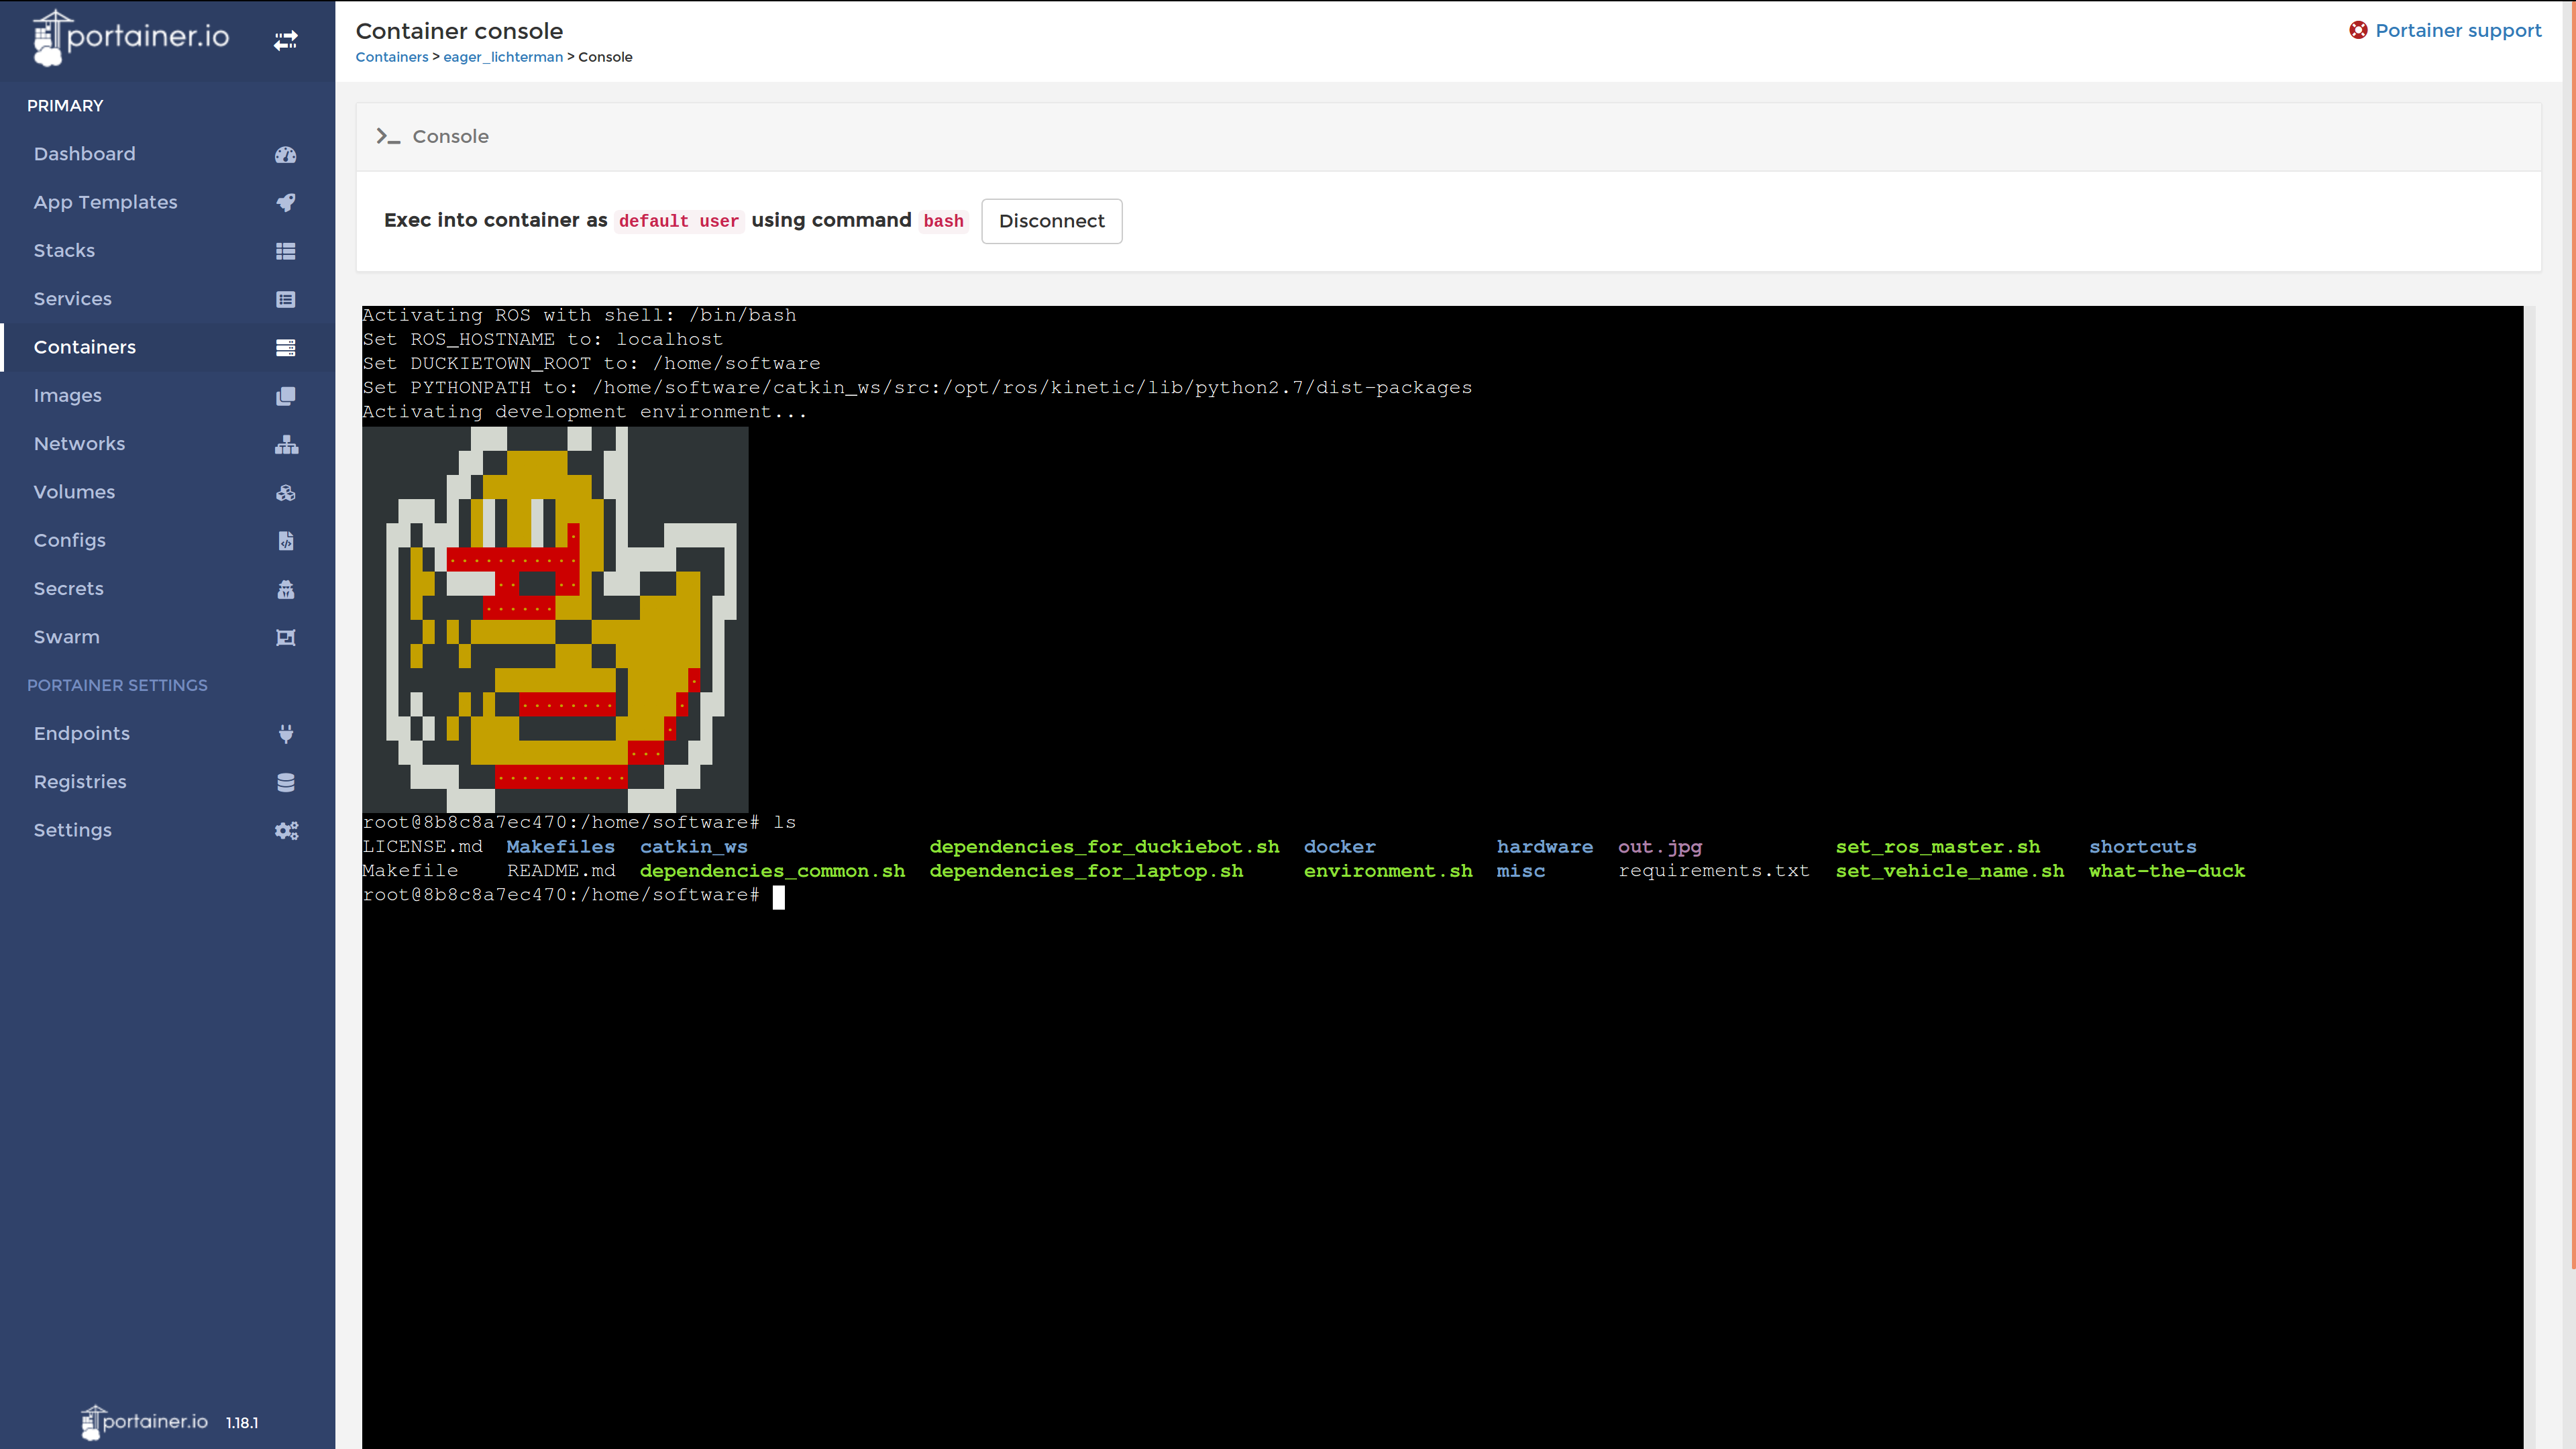
\includegraphics[width=0.80\textwidth]{../figures/portainer_screenshot.png}
    \caption{Browser interface for individual Duckiebots. It is provided by \href{https://www.portainer.io/}{Portainer}, a RESTful web dashboard, which wraps the Docker CLI and offers support for container management, configuration, networking and terminal emulation (shown above). \menu{{\url{http://DUCKIEBOT_NAME:9000/#/container/container_name}} > ``\underline{Console}'' \faMousePointer}}
    \label{fig:portainer_ui}
\end{figure}

\subsection{Testing ROS}

\noindent To verify Docker is working properly, launch a remote container, interactively, like so:

\begin{pclisting}
~$ docker (*\hl{-H DUCKIEBOT\_NAME}*) run -it --privileged --net host \
   duckietown/rpi-ros-kinetic-base:master18
\end{pclisting}
%
The \inline{-H} flag indicates a remote Docker host on the local area network where the Docker command should be executed. For the \inline{DUCKIEBOT\_NAME} address to work, mDNS must be properly configured in the network settings, otherwise an IP address is required.

\subsection{Build and deployment}

Docker images can be cross-compiled by enclosing the ARM-specific portion of the \inline{Dockerfile} with the \inline{RUN [ "cross-build-start" ]} and \inline{RUN [ "cross-build-end" ]} instructions. The following command can be used for deployment:

\begin{pclisting}
~$ docker save TAG_NAME | ssh -C duckie@DUCKIEBOT_NAME docker load
\end{pclisting}
%
Alternately, it is possible to build directly on ARM devices by creating a file named \inline{Dockerfile.arm}, adding a base image and build instructions, then running the command:

\begin{rpilisting}
~$ docker build --file=FILE_PATH/Dockerfile.arm --tag [TAG NAME] .
\end{rpilisting}
%
\subsection{Multi-architecture support}

As of Docker version 18.09.6, ARM-specific \inline{Dockerfile}s will not build on x86 machines.\hspace{-.08em}\footnote{With the exception of the Mac OS Docker client, which offers multi-architecture support. Further details on multiarch support can be found here: \url{https://docs.docker.com/docker-for-mac/multi-arch/} More recent versions of Docker Desktop for Mac OS and Windows have introduced native ARM emulation: \url{https://engineering.docker.com/2019/04/multi-arch-images/}}, and attempting to build one will produce the following error when running \inline{docker build}:

\begin{pclisting}
standard_init_linux.go:175: exec user process caused "exec format error"
\end{pclisting}
%
In order to circumvent this restriction, ARM-specific \inline{Dockerfile}s can be ported to run on x86 by using the \inline{RUN [ "cross-build-start" ]} and \inline{RUN [ "cross-build-end" ]} directives, after the \inline{FROM} and before the \inline{CMD} instructions. See \autoref{subsec:balena} for further details.

All Duckietown Docker images ship with the \href{https://www.qemu.org}{QEMU}~\citep{bellard2005qemu} emulator -- this allows us to run ARM images on x86 directly. To run a pure compute ROS node (i.e.\ one that does not require any camera or motor access) on an x86 platform, developers must supply a custom entrypoint to Docker when running the image using the entrypoint flag as follows:

\begin{pclisting}
~$ docker run ... (*\hl{-{}-entrypoint=qemu3-arm-static}*) IMAGE [RUN_COMMAND]
\end{pclisting}
%
Here, \inline{RUN\_COMMAND} may be a shell such as \inline{/bin/bash} or another command such as \inline{/bin/bash -c "roscore"}. The entrypoint refers to the ARM emulator packaged within the base image, \inline{duckietown/rpi-ros-kinetic-base}, which allows ARM binaries to be run on x86 hosts.

\subsection{Running a simple HTTP file server}

\noindent All persistent data is stored in \inline{/data}. To serve this directory, a web server is provided:

\begin{pclisting}
~$ docker -H DUCKIEBOT_NAME run -d -v /data:/data -p 8082:8082 \
   duckietown/rpi-simple-server:master18
\end{pclisting}
%
To then access this directory, visit the following URL: \url{http://DUCKIEBOT_NAME:8082/}

\subsection{Camera testing}

\noindent The following command can be used to test the camera is working properly. By default, images will be hosted at: \url{http://DUCKIEBOT_NAME:8081/figures/image.jpg}

\begin{pclisting}
~$ docker -H DUCKIEBOT_NAME run -d --privileged -v /data:/data -p 8081:8081
   duckietown/rpi-docker-python-picamera:master18
\end{pclisting}
%
Like most commands, a Python-based shell is provided for the user's convenience:

\begin{dtslisting}
dt> duckiebot demo --demo_name camera --duckiebot_name DUCKIEBOT_NAME
\end{dtslisting}
%
\subsection{Graphical User Interface tools}

To use GUI tools, one must first allow incoming X connections from the host. On Linux hosts, this can be done by running \inline{xhost +} outside Docker.\hspace{-.08em}\footnote{See \url{https://wiki.ros.org/docker/Tutorials/GUI#The_safer_way} for a more secure alternative.} A container with common ROS GUI plugins can be started with following command:

\begin{pclisting}
~$ docker run -it --rm --net host \
   --env ROS_MASTER_URI=http://DUCKIEBOT_IP:11311 \
   --env ROS_IP=LAPTOP_IP \
   --env="DISPLAY" \
   --env="QT_X11_NO_MITSHM=1" \
   --volume="/tmp/.X11-unix:/tmp/.X11-unix:rw" \
   duckietown/rpi-gui-tools
\end{pclisting}
%
Packaged within this image are common ROS plugins which can be run on graphical environments. A shell wrapper is also provided for convenience:

\begin{dtslisting}
dt> start_gui_tools DUCKIEBOT_NAME rqt_image_view
\end{dtslisting}
%
The above command opens a ROS shell that will connect to the \inline{DUCKIEBOT}'s ROS master node. To test the ROS connection works, run \inline{roswtf}.

\subsection{Remote control}

\noindent The following container launches the joystick demo (USB joystick must be connected):

\begin{pclisting}
~$ docker -H DUCKIEBOT_NAME run --privileged --net host -v /data:/data \
   duckietown/rpi-duckiebot-joystick-demo:master18
\end{pclisting}
%
\begin{dtslisting}
dt> duckiebot demo --demo_name joystick --duckiebot_name DUCKIEBOT_NAME
\end{dtslisting}
%
\begin{dtslisting}
dt> duckiebot keyboard_control DUCKIEBOT_NAME
\end{dtslisting}
%
\subsection{Camera calibration}

\noindent The following container will launch the extrinsic calibration procedure:

\begin{pclisting}
~$ docker -H DUCKIEBOT_NAME run -it --privileged --net host (*\hl{-v /data:/data}*)
   duckietown/rpi-duckiebot-calibration:master18
\end{pclisting}
%
Passing \inline{-v /data:/data} is necessary so that all calibration settings will be preserved. When placed on the calibration pattern, the following commands will initiate an interactive calibration sequence for the camera.

\begin{dtslisting}
dt> duckiebot calibrate_extrinsics DUCKIEBOT_NAME
\end{dtslisting}
%
\begin{dtslisting}
dt> duckiebot calibrate_intrinsics DUCKIEBOT_NAME
\end{dtslisting}
%
\subsection{Wheel calibration}

\noindent To calibrate the gain and trim of the wheel motors, the following commands are needed:

\begin{dtslisting}
dt> duckiebot demo --demo_name base --duckiebot_name NAME
\end{dtslisting}
\begin{pclisting}
~$ rosservice call /DUCKIEBOT_NAME/inverse_kinematics_node/set_gain --GAIN
\end{pclisting}
\begin{pclisting}
~$ rosservice call /DUCKIEBOT_NAME/inverse_kinematics_node/set_trim --TRIM
\end{pclisting}
%
\subsection{Lane following}

\noindent Once calibrated, the lane following demo can be launched as follows:

\begin{pclisting}
~$ docker -H DUCKIEBOT_NAME run -it --privileged --net host -v /data:/data
   duckietown/rpi-duckiebot-lanefollowing-demo:master18
\end{pclisting}
%
\begin{dtslisting}
dt> duckiebot demo --demo_name lane_following --duckiebot_name DUCKIEBOT_NAME
\end{dtslisting}
%
\section{Retrospective}\label{sec:retrospective}

One problem encountered during the development of Duckietown's Docker infrastructure was the matter of whether to store source code inside or outside the container (e.g. as described in \autoref{subsec:volume_sharing}). If stored externally, a developer can still load source code in a shared volume and rebuild on container startup. Both approaches can produce reproducible artifacts if properly versioned, but Docker images launch more quickly when images are fully prebuilt and tend to be more inspectable with sources included.

Initially, we made the explicit decision to ship user source code directly inside the image. As a consequence, any modifications to the source code would trigger a subsequent rebuild, tying the sources and Docker image together. While including sources enables easier troubleshooting and diagnostics, it also adds some friction during development, which caused users to struggle with environment setup and Docker configuration issues.

\begin{figure}
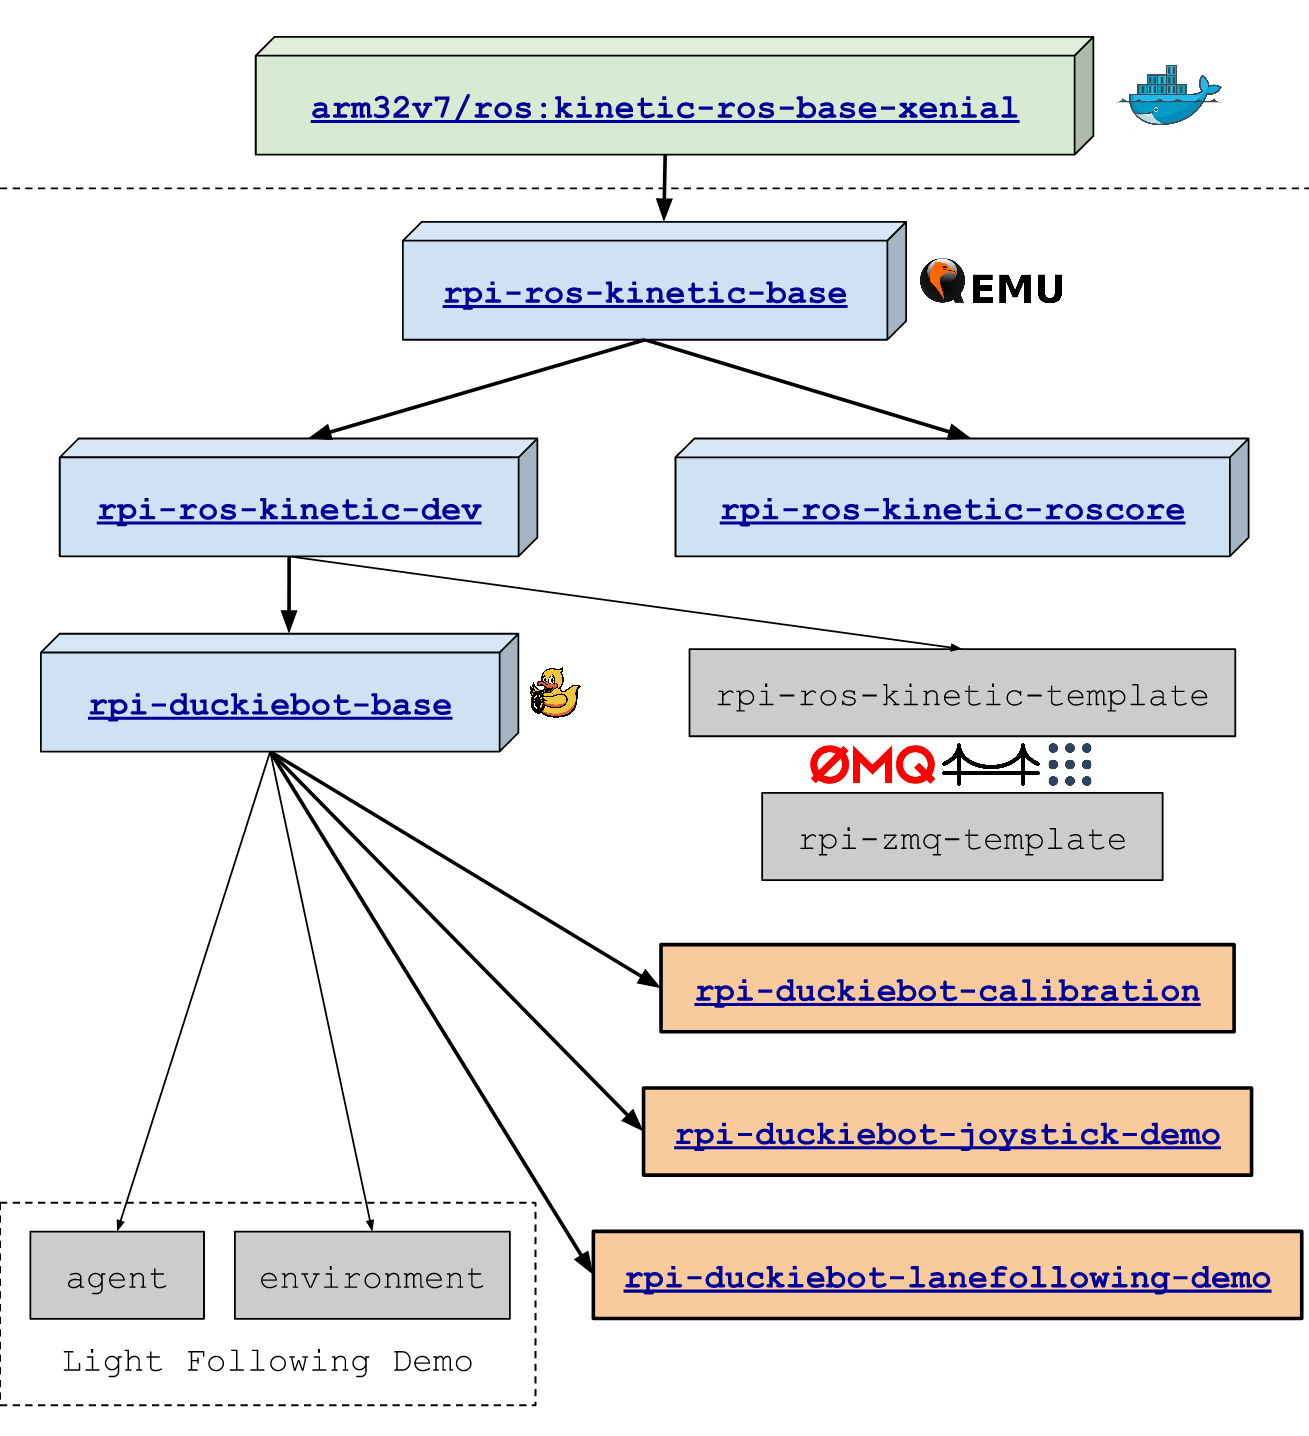
\includegraphics[width=0.80\textwidth]{../figures/image_provenance.png}
\caption{Early prototype of the Docker image hierarchy. Chaining unversioned autobuilds without disciplined unit testing creates a potential domino effect which allows breaking changes to propagate downstream, resulting in a cascade of silent failures.}
    \label{fig:early_prototype}
\end{figure}

The root cause of this friction was a product of imprecise versioning and over-automation. As version tags were initially omitted, all images were built and pulled from latest commit on the mainline development branch. The auto-build feature of the CI server caused upstream modifications to cascade to downstream images. Our short-term solution was to disable auto-building, and push local builds to the server manually, however fixing it required us to rethink the role of versioning and testing Docker builds in the CI toolchain.

\begin{figure}
    
\includegraphics[width=0.40\textwidth]{../figures/aido_logo.png}
    \caption{The \href{https://www.duckietown.org/research/ai-driving-olympics}{AI Driving Olympics}, a primary use case for the system described above.}
    \label{fig:aido_logo}
\end{figure}

A more stable solution is to store all sources on the local development environment and rebuild the image only when its upstream dependencies change. The image only contains its compiled upstream dependencies and is only paired with source code at runtime.

One of the primary use cases for the Duckietown container infrastructure is a biannual autonomous robotics competition called the AI Driving Olympics~\citep{aido2018} (AIDO). To participate, competitors must submit a Docker image (various templates are provided for \href{https://github.com/duckietown/challenge-aido_LF-baseline-RL-sim-pytorch}{reinforcement learning}, \href{https://github.com/duckietown/challenge-aido_LF-baseline-IL-logs-tensorflow}{imitation learning} and \href{https://github.com/duckietown/challenge-aido_LF-template-ros}{classical robotics}). The submitted image, together with a Git repository and a commit hash, constitutes an AIDO submission. The submission is retrieved by the organizers and evaluated on a random map in Duckietown's \href{https://github.com/duckietown/gym-duckietown}{simulator}~\citep{gym_duckietown}. This evaluation produces a numerical score in several categories. Valid submissions may also be run on a physical \textit{robotarium}. The highest ranking submissions are evaluated in a final round at NeurIPS and ICRA.

\subsection{Remarks on security}

An unfortunate technical shortcoming of the Docker system is its reliance on superuser privileges. While Docker takes a variety of preventative measures to ensure container inhabitants cannot gain escalated privileges, numerous breakout attacks have been discovered~\citep{martin2018docker} in the wild. Any process which can circumvent container security gains unfettered access to the host OS, making Docker especially unsuitable for deployment on cloud, grid, and cluster computing environments.

Furthermore, Docker provides a mechanism to bypass its own security measures, allowing container applications to run as if they were root processes on the host OS: the \href{https://docs.docker.com/engine/reference/run/#security-configuration}{\inline{-{}-privileged} flag}. This feature, alongside the fact that most Docker users are unqualified to audit upstream images, which are liable to include packages of dubious provenance~\citep{martin2018docker}, makes Docker particularly troublesome for shared-computing environments.

Docker's unnecessarily high privileges and susceptibility for misuse are serious issues. While operator error may be partly at fault, these vulnerabilities are primarily the result of poor implementation choices. Docker's flagrant violation of the principle of least privilege~\citep{saltzer1975protection} effectively compromises the entire Linux security model.

To address these issues, various container platforms, including \href{https://docs.nersc.gov/programming/shifter/overview/}{Shifter}~\citep{gerhardt2017shifter} and \href{https://sylabs.io/docs/}{Singularity}~\citep{kurtzer2017singularity}, have emerged and gained traction in the scientific computing community, owing to their lower privileges and compatibility with legacy Linux distributions used by many academic computing environments. Since then, Docker has also introduced a \href{https://engineering.docker.com/2019/02/experimenting-with-rootless-docker/}{rootless mode}, but it remains experimental at the time of writing this thesis.

\section{Conclusion}

In this chapter we have taken a guided tour through the process of containerization and demonstrated the effectiveness of containers for building reproducible robotics software -- a key step in the broader quest for experimental reproducibility. We offer a set of best practices and lessons learned during the design, development and deployment of Docker containers for the Duckietown~\citep{paull2017duckietown} platform. The author wishes to thank Rusi Hristov for his invaluable technical assistance during the preliminary stages of this project.

%\mediumrare{\chapter{An application for autonomous robotics}\label{ch:case-study}}
%
%\setlength{\epigraphwidth}{0.80\textwidth}
%\epigraph{``Thus, I came to the conclusion that the designer of a new system must not only be the implementor and the first large-scale user; the designer should also write the first user manual. The separation of any of these four components would have hurt TeX significantly. If I had not participated fully in all these activities, literally hundreds of improvements would never have been made, because I would never have thought of them or perceived why they were important.''}{\begin{flushright}-- Donald E.~\citet{knutherrors}, \href{https://yurichev.com/mirrors/knuth1989.pdf}{\textit{The Errors of \TeX}}\end{flushright}}
%
%As a case study, we have implemented a mobile application using ROS, Docker, and Android, using the tools proposed in \autoref{ch:hatchery}--\autoref{ch:ducker}. The source code for this section can be found at the following URL: \url{https://github.com/breandan/duckietown-rc}
%
%\section{Design}
%
%Hatchery is compatible with most IDEs built on the IntelliJ Platform, including \href{https://developer.android.com/studio}{Android Studio}, the official IDE for Android mobile development. To use ROS-specific features from within Android Studio, ensure the Hatchery plugin is installed as described in ~\autoref{subsec:installation}. First create a new ROS Android project or clone an existing one from version control. Then create a symbolic link inside the Android project's root directory to the ROS project:
%%
%\begin{pclisting}
%~$ ln -s /absolute/path/to/ros/project /android/project
%\end{pclisting}
%%
%Import the project in Android Studio via \menu{File > New > Project from Existing sources\textellipsis}.  Now, the ROS project can be managed from within Android Studio.\vspace{10pt}\\
%%
%\begin{centering}
%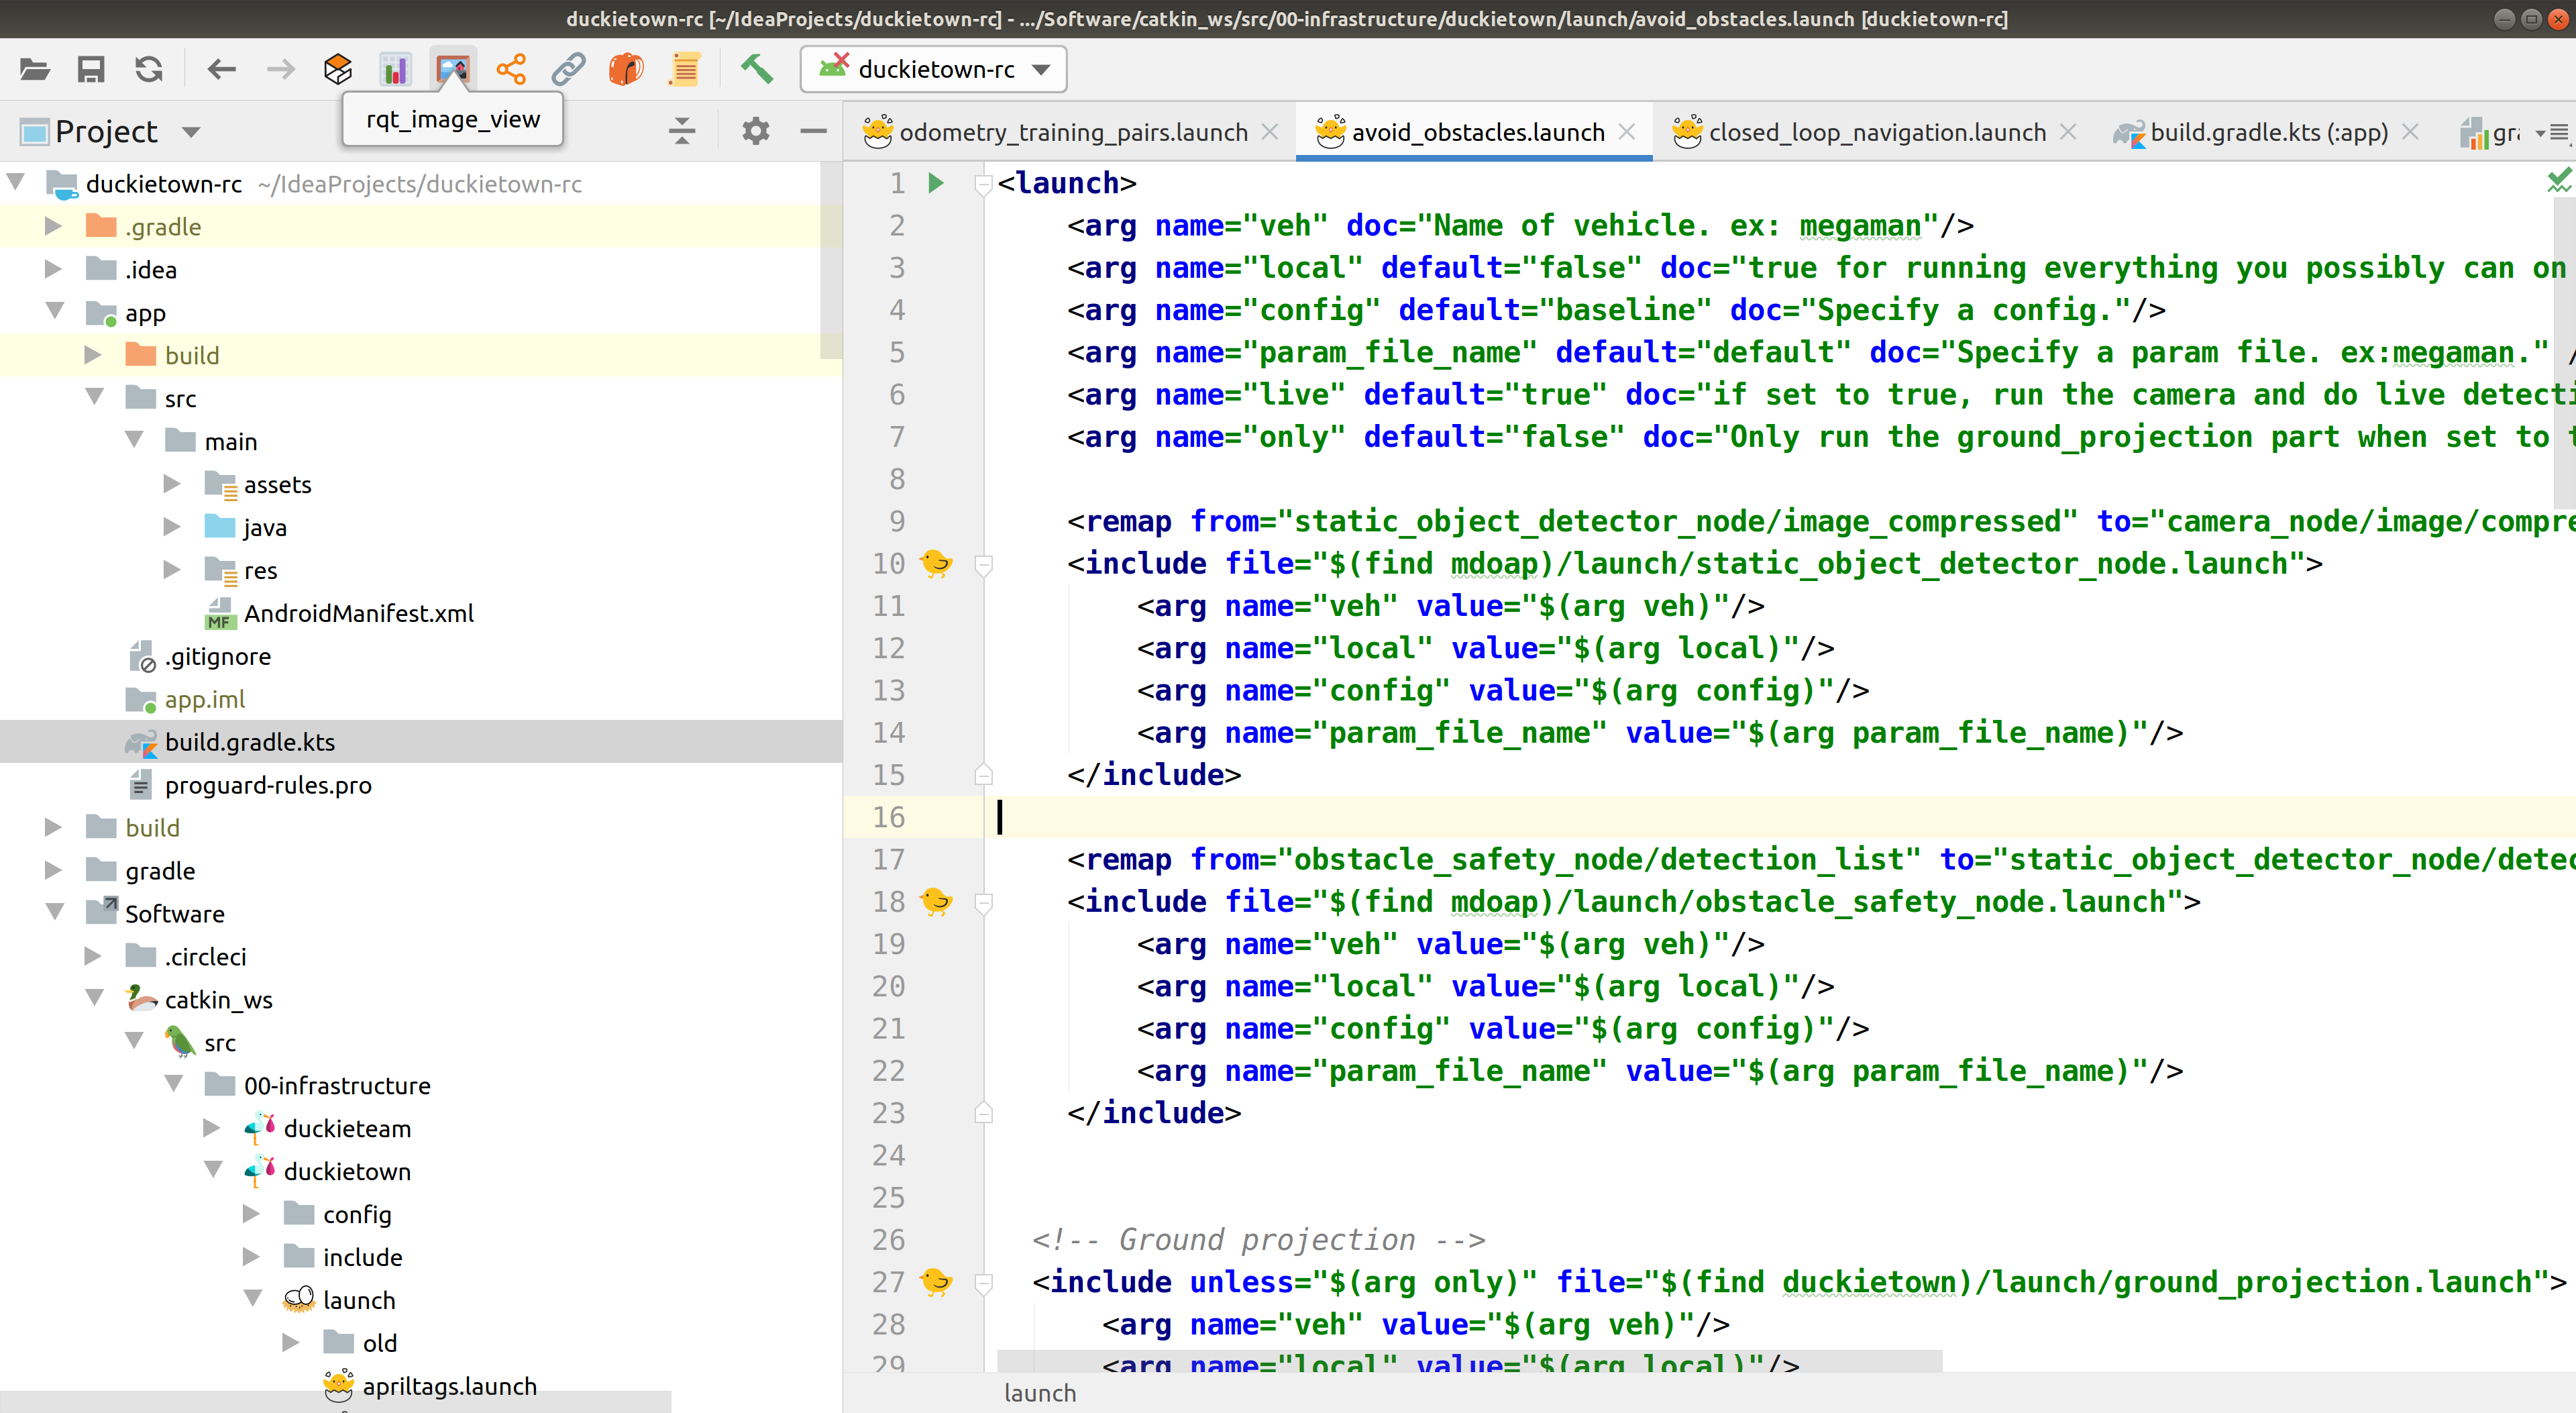
\includegraphics[width=\textwidth]{../figures/hatchery_android.png}
%\end{centering}\vspace{10pt}
%%
%Running ROS nodes on desktop or embedded devices follows the same procedure as ordinary rospy projects. Running ROS nodes on Android devices, however, requires the use of \href{https://wiki.ros.org/rosjava}{rosjava}, a pure Java implementation of the ROS messaging protocol. The rosjava project provides examples of various \href{https://github.com/rosjava/android_apps}{Android applications}, including a basic Android UI and support for communicating with networked ROS nodes.
%
%ROS Android applications can be run on either a physical Android or Android Virtual Device (AVD). To enable bidirectional communication between an external node and AVD ROS node, use the following commands to open a \inline{telnet} connection and configure port forwarding, as described in the \href{https://developer.android.com/studio/run/emulator-networking#consoleredir}{Android developer documentation}:
%%
%\begin{pclisting}
%~$ telnet localhost 5554
%~$ redir add tcp:11311:11311
%\end{pclisting}
%
%\section{Implementation}
%
%Due to Android's Kotlin interoperability, Kotlin libraries are directly usable inside Android projects. To use Kotlin$\nabla$ in an Android project, first add a custom Maven repository to the project's \inline{build.gradle.kts} file:
%%
%\begin{kotlinlisting}
%repositories {
%    maven("https://maven.pkg.github.com/breandan/kotlingrad")
%}
%\end{kotlinlisting}
%%
%Then add the \href{https://github.com/breandan/kotlingrad/packages}{latest version of Kotlin$\nabla$} to \inline{dependencies} in the \inline{build.gradle.kts} file:
%%
%\begin{kotlinlisting}
%dependencies {
%    compile("edu.umontreal:kotlingrad:<VERSION>")
%}
%\end{kotlinlisting}
%%
%Kotlin$\nabla$ can now be used just like an ordinary library in any Android application.
%
%\section{Testing and validation}
%
%Verified using property-based testing.\vspace{10pt}\\
%%
%\begin{centering}
%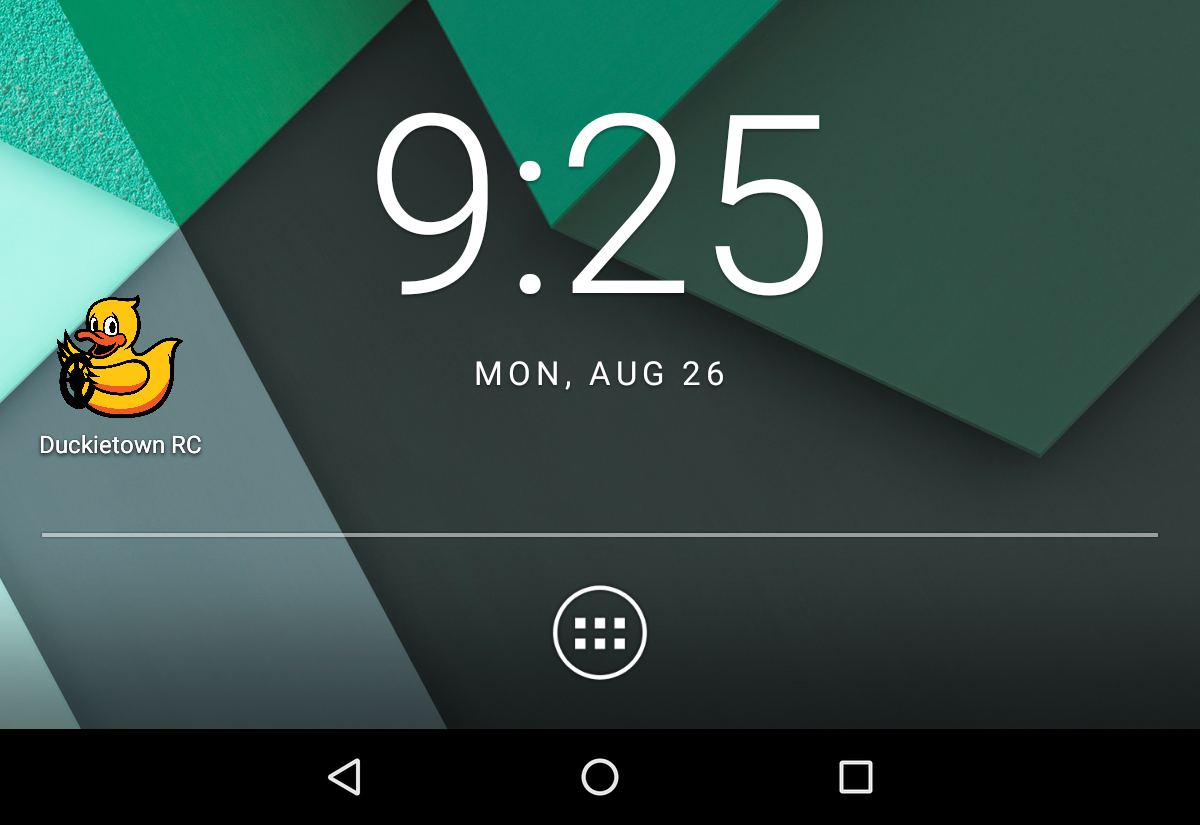
\includegraphics[width=\textwidth]{../figures/android_screenshot.png}
%\end{centering}
%
%\section{Containerization}
%
%Deployed and CI-tested using Docker.
%
%\section{Conclusion}
%
%In this chapter, we illustrate one feasible application of the toolchain previously proposed. As a toy example, it is primarily intended to be illustrative in nature.

\chapter{Conclusion}\label{ch:conclusion}
\setlength{\epigraphwidth}{0.90\textwidth}
\epigraph{``We are all shaped by the tools we use, in particular: the formalisms we use shape our thinking habits, for better or for worse, and that means that we have to be very careful in the choice of what we learn and teach, for unlearning is not really possible.''}{\begin{flushright}--Edsger W. \citet{dijkstra2000answers}, \href{https://www.cs.utexas.edu/~EWD/transcriptions/EWD13xx/EWD1305.html}{\textit{Answers to questions from students of Software Engineering}}\end{flushright}}

In this work, we explored four different programming tools from software engineering for the development of intelligent systems, broadly addressing cognitive complexity arising in various stages of Royce's Waterfall method~\autoref{fig:waterfall_model}. These tools have varying degrees of practicality, from highly experimental (adversarial testing of differentiable programs ~\autoref{ch:difftest}) to more pragmatic (containerization ~\autoref{ch:ducker}). In each, we provide some motivating examples and use cases which demonstrate key deficiencies in the current state of programming tools for intelligent systems and propose candidate solutions which address a few of those shortcomings. While we certainly hope that intelligent system programmers (e.g. roboticists and machine learning practitioners) may derive some value from the tools themselves, our intention is to be \textit{instructive} rather than \textit{prescriptive}.

By building tools and validating their effectiveness for toy applications, we hope that middleware and tools developers will carefully consider the cognitive complexity which software abstraction can introduce and the importance of notational and denotational design practices. In addition, we hope that by providing some examples illustrating programming tools in the ML/IS domain, developers will be inspired to re-imagine the possibilities for computer-aided programming towards the design of intelligent systems and begin to design better tools for developers working on similar problems.

By complementing the cognitive abilities of human programmers -- who excel at creative problem solving and high-level abstract reasoning -- with the low-level symbolic processing capabilities of programming tools, we can accelerate the design, development and validation of intelligent systems in real-world applications. This process, we argue, deserves more specific tools than general-purpose programming due to the opportunities and challenges which intelligent systems present and the unique interplay of human-machine intelligence.

As we start to engineer autonomous systems which take increasingly human decisions, programmers will play a critical role in shaping the behavior and dynamics of these systems. In order to build trustworthy autonomous systems, it will be important to have tools which enable humans to understand and inform their behavior in a more rigorous manner than monitoring training curves and performing hyperparameter sweeps. This requires us to actively rethink the programming model in machine learning to incorporate human knowledge, e.g. using differentiable programming and type theory (\autoref{ch:kotlingrad}) or building custom tools which incorporate automatic reasoning capabilities and visualization tools (e.g. customized run and debugging assistance \autoref{ch:hatchery}). Finally, to make the resulting software artifacts more reproducible will require sound build systems and best practices for reproducible software installation and configuration (\autoref{ch:ducker}).

\section{Future work}

\subsection{Requirements engineering}

Traditional software engineering has followed a rigorous process model and testing methodology. This model has guided the development of traditional software engineering, intelligent systems will need to re-imagine these ideas to build systems which adapt to their environment. Intelligent systems are trained on objective functions, which are typically one- or low-dimensional metrics for evaluating the performance of the system. Most often, these take the form of a single or small set of criteria, such as an \textit{error} or \textit{loss} which can represent descriptive phenomena such as latency, safety, energy efficiency or any number of objective measures.

In traditional software engineering, it is reasonable to assume the people who are implementing a system have some implicit knowledge and are generally well-intentioned human beings working towards a common goal. When building an intelligent system, it is not unreasonable to assume is that the entity implementing our requirements is a na\"ive but powerful genie. When given an optimization metric, it will take every available shortcut to satisfy that criteria. If we are not careful about engineering the requirements correctly, this entity can produce a system that does not work, or has unintended consequences.

When building an intelligent system developers must first ask, ``What are the requirements of the system?'' This question is often the most troublesome part, because the requirements must not be fuzzy specifications as often the case in software engineering, but precise constraints on the space of solutions. In a strict sense, specifying the requirements is often indistinguishable from implementing the system. With the right language abstractions (e.g.\ declarative programming), requirements and implementation can take the same notation. These ideas have been explored in recent decades with declarative languages like SQL and Prolog.

For example, in the design of a web-based advertisement recommendation system, we can optimize for various objectives such as click rate, engagement, sales conversion. So long as we can measure these parameters, modern function approximators can optimize for any single criterion or combination thereof. Much of the work involved in machine learning is finding representations which are suitable for downstream tasks, and prevent unintended consequences. For example, by optimizing for click rate, we create an artificial market for click bots. Similarly, in self-driving vehicles, we often want to optimize for passenger safety. However, by doing so na\"ively, we create a vehicle that never moves, or always yields to nearby vehicles.

\bibliography{thesis}
\bibliographystyle{plainnat}

\appendix
\chapter{Type-safe differentiable programming}

\section{Grammar}

Below is an approximately complete BNF grammar for Kotlin$\nabla$:

\newcommand{\mor}{\ensuremath{\;\mid\;}}
\newcommand{\code}[1]{\ensuremath{\text{\inline{#1}}}}
\newcommand{\bnfrl}[1]{\ensuremath{\langle#1\rangle}}
\begin{eqnarray*}
\bnfrl{type} & ::= & \code{Double} \mor \code{Float} \mor \code{Int} \mor \code{BigInteger} \mor \code{BigDouble} \\
\bnfrl{nat} & ::= & \code{1} \mor \ldots \mor \code{99} \\
\bnfrl{output} & ::= & \code{Fun<}\bnfrl{type}\code{Real>} \mor \code{VFun<}\bnfrl{type}\code{Real,}\bnfrl{nat}\code{>} \mor \code{MFun<}\bnfrl{type}\code{Real,}\bnfrl{nat}\code{,}\bnfrl{nat}\code{>} \\
\bnfrl{int} & ::= & \code{0} \mor \bnfrl{nat}\bnfrl{int} \\
\bnfrl{float} & ::= & \bnfrl{int}\code{.}\bnfrl{int} \\
\bnfrl{num} & ::= & \bnfrl{type}\code{(}\bnfrl{int}\code{)} \mor \bnfrl{type}\code{(}\bnfrl{float}\code{)} \\
\bnfrl{var} & ::= & \code{x} \mor \code{y} \mor \code{z} \mor \code{ONE} \mor \code{ZERO} \mor \code{E} \mor \code{Var()}} \\
\bnfrl{signOp} & ::= & \code{+} \mor \code{-} \\
\bnfrl{binOp} & ::= & \bnfrl{signOp} \mor \code{*} \mor \code{/} \mor \code{pow} \\
\bnfrl{trigOp} & ::= & \code{sin} \mor \code{cos} \mor \code{tan} \mor \code{asin} \mor \code{acos} \mor \code{atan} \mor \code{asinh} \mor \code{acosh} \mor \code{atanh} \\
\bnfrl{unaryOp} & ::= & \bnfrl{signOp} \mor \bnfrl{trigOp} \mor \code{sqrt} \mor \code{log} \mor \code{ln} \mor \code{exp} \\
\bnfrl{exp} & ::= & \bnfrl{var} \mor \bnfrl{num} \mor \bnfrl{unaryOp}\bnfrl{exp} \mor \bnfrl{var}\bnfrl{binOp}\bnfrl{exp} \mor \code{(} \bnfrl{exp} \code{)} \\
\bnfrl{expList} & ::= & \bnfrl{exp} \mor \bnfrl{exp} \code{,} \bnfrl{expList} \\
\bnfrl{linOp} & ::= & \bnfrl{signOp} \mor \code{*} \mor \code{ dot } \\
\bnfrl{vec} & ::= & \code{Vec(} \bnfrl{expList} \code{)} \mor \code{Vec} \bnfrl{nat} \code{(} \bnfrl{expList} \code{)} \\
\bnfrl{vecExp} & ::= & \bnfrl{vec} \mor \bnfrl{signOp}\bnfrl{vecExp} \mor \bnfrl{exp} \code{*} \bnfrl{vecExp} \mor \bnfrl{vec} \bnfrl{linOp} \bnfrl{vecExp} \\
&&\bnfrl{vecExp}\code{.norm(}\bnfrl{int}\code{)} \\
\bnfrl{mat} & ::= & \code{Mat} \bnfrl{nat} \code{x} \bnfrl{nat} \code{(} \bnfrl{expList} \code{)} \\
\bnfrl{matExp} & ::= & \bnfrl{mat} \mor \bnfrl{signOp}\bnfrl{matExp} \mor \bnfrl{exp}\bnfrl{linOp}\bnfrl{matExp} \mor \\
&&\bnfrl{vecExp}\bnfrl{linOp}\bnfrl{matExp} \mor \bnfrl{mat} \bnfrl{linOp} \bnfrl{matExp} \\
\bnfrl{anyExp} & ::= & \bnfrl{exp} \mor \bnfrl{vecExp} \mor \bnfrl{matExp} \mor \bnfrl{derivative} \mor \bnfrl{invocation} \\
\bnfrl{bindings} & ::= & \bnfrl{exp} \code{ to } \bnfrl{exp} \mor \bnfrl{exp} \code{ to } \bnfrl{exp} \code{,} \bnfrl{bindings} \\
\bnfrl{invocation} & ::= & \bnfrl{anyExp} \code{(} \bnfrl{bindings} \code{)} \\
\bnfrl{derivative} & ::= & \code{d(} \bnfrl{anyExp} \code{) / d(} \bnfrl{exp} \code{)} \mor \bnfrl{anyExp} \code{.d(} \bnfrl{exp} \code{)} \mor \bnfrl{anyExp} \code{.d(} \bnfrl{expList} \code{)} \\
\bnfrl{gradient} & ::= & \bnfrl{exp} \code{.grad()}
\end{eqnarray*}


\section{Linear regression}

\noindent Recall the matrix equation for linear regression, where $\mathbf{X}: \mathbb{R}^{m \times n}$ and $\bm\Theta: \mathbb{R}^{n \times 1}$:
%
\begin{equation}
\mathbf{\hat f}(\mathbf{X}; \bm\Theta) = \mathbf{X}\bm\Theta
\end{equation}
%
Imagine we are given the following dataset:
%
\begin{equation}
\mathbf{X} =
\begin{bmatrix}
\mathbf{x}_1 \\
\vdots \\
\mathbf{x}_m
\end{bmatrix} =
\begin{pmatrix}
1 & \ldots & x_{1n} \\
\vdots & \ddots & \vdots \\
1 & \ldots & x_{mn}
\end{pmatrix},
\mathbf{Y} =
\begin{bmatrix}
y_2 \\
\vdots \\
y_m
\end{bmatrix}
\end{equation}
%
Our goal in ordinary least squares (OLS) linear regression is to minimize the loss, or error between the data and the model's prediction:
%
\begin{equation}
\mathcal{L}(\mathbf{X}, \mathbf{Y}; \bm\Theta) = ||\mathbf{Y} - \mathbf{\hat f}(\mathbf{X}; \bm\Theta)||^2
\end{equation}
%
\begin{equation}
\bm\Theta^* = \underset{\bm\Theta}{\operatorname{argmin}}\mathcal{L}(\mathbf{X}, \mathbf{Y}; \bm\Theta)
\end{equation}

\subsection{Finite difference method}\label{sec:fdm}

First, we consider the scalar case, where $\mathbf{\hat f}(\mathbf{X}; \bm\Theta) = \hat f(x; \theta_2, \theta_1) = \theta_2 x + \theta_1$. Since $\mathbf{X}, \mathbf{Y}$ are considered to be fixed, we can rewrite $\mathcal{L}(\mathbf{X}, \mathbf{Y}; \bm\Theta)$ as simply:
%
\begin{equation}
\mathcal{L}(\bm\Theta) = \mathcal{L}(\theta_2, \theta_1) = \frac{1}{m}\sum_{i=1}^m(y_i - (\theta_2 x_i + \theta_1))^2
\end{equation}
%
To find the minimizer of $\mathcal{L}(\bm\Theta)$, we need $\nabla_{\bm\Theta}\mathcal{L} = \lbrack \frac{\partial\mathcal{L}}{\partial \theta_2}, \frac{\partial\mathcal{L}}{\partial \theta_1}\rbrack$. There are various ways to compute this. First, let's see FDM with centered differences:
%
\begin{align}
\frac{\partial\mathcal{L}}{\partial \theta_1} & = \underset{h \rightarrow 0}{\operatorname{lim}} \frac{\sum_{i=1}^m\left(y_i - \left(\theta_2 x_i + \theta_1 + h\right)\right)^2 - \sum_{i=1}^m\left(y_i - \left(\theta_2 x_i + \theta_1 - h\right)\right)^2}{2hm} \\ & = \underset{h \rightarrow 0}{\operatorname{lim}} \frac{1}{2hm}\sum_{i=1}^m\left(y_i - \left(\theta_2 x_i + \theta_1 + h\right)\right)^2 - \left(y_i - \left(\theta_2 x_i + \theta_1 - h\right)\right)^2 \\
\frac{\partial\mathcal{L}}{\partial \theta_2} & = \underset{h \rightarrow 0}{\operatorname{lim}} \frac{\sum_{i=1}^m\left(y_i - \left((\theta_2 + h) x_i + \theta_1\right)\right)^2 - \sum_{i=1}^m\left(y_i - \left(\left(\theta_2 - h\right) x_i + \theta_1\right)\right)^2}{2hm} \\ & = \underset{h \rightarrow 0}{\operatorname{lim}} \frac{1}{2hm}\sum_{i=1}^m\left(y_i - \left(\left(\theta_2 + h\right) x_i + \theta_1\right)\right)^2 - \left(y_i - \left(\left(\theta_2 - h\right) x_i + \theta_1\right)\right)^2
\end{align}
%
Using computer algebra, the above equations can be simplified considerably:
%
\begin{align}
\frac{\partial\mathcal{L}}{\partial \theta_1} & = \underset{h \rightarrow 0}{\operatorname{lim}} \frac{1}{2hm}\sum_{i=1}^m\left(4h ( \theta_1 +  \theta_2 x_i - y_i)\right) \label{eq:dL_dtheta0} \\
& = \boxed{\frac{2}{m}\sum_{i=1}^m\left(\theta_1 + \theta_2 x_i - y_i\right)} \\
\frac{\partial\mathcal{L}}{\partial \theta_2} & = \underset{h \rightarrow 0}{\operatorname{lim}} \frac{1}{2hm}\sum_{i=1}^m\left(4hx_i (\theta_2 x_i + \theta_1 - y_i)\right) \label{eq:dL_dtheta1} \\
& = \boxed{\frac{2}{m}\sum_{i=1}^m(x_i)(\theta_2 x_i + \theta_1 - y_i)}
\end{align}
%
\begin{enumerate}
    \item[] \autoref{eq:dL_dtheta0}: \url{https://www.wolframalpha.com/input/?i=(y_i-((%CE%B8_2%2Bh)x_i%2B%CE%B8_1))%5E2-(y_i-((%CE%B8_2-h)x_i%2B%CE%B8_1))%5E2}
    \item[] \autoref{eq:dL_dtheta1}: \url{https://www.wolframalpha.com/input/?i=(y_i-(%CE%B8_2*x_i%2B%CE%B8_1%2Bh))%5E2%E2%88%92(y_i-(%CE%B8_2*x_i%2B%CE%B8_1-h))%5E2}
\end{enumerate}

\subsection{Partial differentiation}

\noindent Alternatively, we can calculate the partials analytically, by applying the chain rule:
%
\begin{align}
\frac{\partial\mathcal{L}}{\partial \theta_1} & = \frac{\partial}{\partial \theta_1}\frac{1}{m}\sum_{i=1}^m(y_i - (\theta_2 x_i + \theta_1))^2 \\ & = \frac{1}{m}\sum_{i=1}^m 2 (y_i - (\theta_2 x_i + \theta_1))\frac{\partial}{\partial \theta_1}(y_i - (\theta_2 x_i + \theta_1)) \\ & = \frac{2}{m}\sum_{i=1}^m(y_i - (\theta_2 x_i + \theta_1))(-1) \\ & = \boxed{\frac{2}{m}\sum_{i=1}^m(\theta_2 x_i + \theta_1 - y_i)}
\end{align}
%
\begin{align}
\frac{\partial\mathcal{L}}{\partial \theta_2} & = \frac{\partial}{\partial \theta_2}\frac{1}{m}\sum_{i=1}^m(y_i - (\theta_2 x_i + \theta_1))^2 \\ & = \frac{1}{m}\sum_{i=1}^m 2(y_i - (\theta_2 x_i + \theta_1)) \frac{\partial}{\partial \theta_2}(y_i - (\theta_2 x_i + \theta_1)) \\ & = \frac{2}{m}\sum_{i=1}^m(y_i - (\theta_2 x_i + \theta_1))(-x_i) \\ & = \boxed{\frac{2}{m}\sum_{i=1}^m(x_i)(\theta_2 x_i + \theta_1 - y_i)}
\end{align}
%
Notice how analytical differentiation gives us the same answer as the \hyperref[sec:fdm]{finite difference method} (this is not by accident), with much less algebra. We can rewrite these two solutions in gradient form, i.e. as a column vector of partial derivatives:
%
\begin{equation}
\nabla_{\bm\Theta}\mathcal{L} =
\begin{bmatrix}
\frac{\partial\mathcal{L}}{\partial \theta_1} \\
\frac{\partial\mathcal{L}}{\partial \theta_2}
\end{bmatrix} = \frac{2}{m}
\begin{bmatrix}
\sum_{i=1}^m(\theta_2 x_i + \theta_1 - y_i) \\ \sum_{i=1}^m(x_i)(\theta_2 x_i + \theta_1 - y_i)
\end{bmatrix}
\end{equation}

\subsection{Matrix solution}

Having reviewed the scalar procedure for linear regression, let us now return to the general form of $\mathcal L(\bm\Theta)$. Matrix notation allows us to simplify the loss considerably:
%
\begin{align}
\mathcal L(\bm\Theta) & = \frac{1}{m} (\mathbf Y - \mathbf X \bm\Theta)^\intercal(\mathbf Y - \mathbf X \bm\Theta) \\ &= \frac{1}{m} (\mathbf Y^\intercal \mathbf Y - \mathbf Y^\intercal \mathbf X \bm\Theta - \bm\Theta^\intercal \mathbf X^\intercal \mathbf Y + \bm\Theta^\intercal \mathbf X^\intercal \mathbf X \bm\Theta) \\ &= \frac{1}{m} (\mathbf Y^\intercal \mathbf Y - 2 \bm\Theta^\intercal \mathbf X^\intercal \mathbf Y + \bm\Theta^\intercal \mathbf X^\intercal \mathbf X \bm\Theta)
\end{align}
%
Matrix notation allows us to derive the gradient and requires far less algebra:
%
\begin{align}
\nabla_{\bm\Theta}\mathcal L(\bm\Theta) & = \frac{1}{m} (\nabla_{\bm\Theta}\mathbf Y^\intercal \mathbf Y - 2 \nabla_{\bm\Theta} \bm\Theta^\intercal \mathbf X^\intercal \mathbf Y + \nabla_{\bm\Theta}\bm\Theta^\intercal \mathbf X^\intercal \mathbf X \bm\Theta) \\ & = \frac{1}{m} ( 0 - 2\mathbf{X}^\intercal \mathbf Y + 2 \mathbf{X}^\intercal \mathbf X \bm\Theta ) \\ & = \boxed{\frac{2}{m} (\mathbf{X}^\intercal \mathbf X \bm\Theta - \mathbf{X}^\intercal \mathbf Y)}
\end{align}
%
For completeness, and to convince ourselves the matrix solution is indeed the same:
%
\begin{align}
& = \frac{2}{m}\left(
\underbrace{\begin{bmatrix}
1 & \ldots & 1 \\
x_1 & \ldots & x_m \\
\end{bmatrix}}_{\mathbf{X}^\intercal}
\underbrace{\begin{bmatrix}
1 & x_1 \\
\vdots & \vdots \\
1 & x_m
\end{bmatrix}}_{\mathbf{X}}
\underbrace{\begin{bmatrix}
\theta_1 \\
\theta_2
\end{bmatrix}}_{\bm\Theta} -
\underbrace{\begin{bmatrix}
1 & \ldots & 1 \\
x_1 & \ldots & x_m \\
\end{bmatrix}}_{\mathbf{X}^\intercal}
\underbrace{\begin{bmatrix}
y_1 \\
\vdots \\
y_m
\end{bmatrix}}_{\mathbf{Y}}\right) \\
& = \frac{2}{m}\left(
\underbrace{\begin{bmatrix}
m & \sum_{i=1}^{m}x_i \\
\sum_{i=1}^{m}x_i & \sum_{i=1}^{m}x_i^2 \\
\end{bmatrix}}_{\mathbf{X}^\intercal\mathbf{X}}
\underbrace{\begin{bmatrix}
\theta_1 \\
\theta_2
\end{bmatrix}}_{\bm\Theta} -
\underbrace{\begin{bmatrix}
\sum_{i=1}^{m}y_i \\
\sum_{i=1}^{m}x_iy_i
\end{bmatrix}}_{\mathbf{X}^\intercal\mathbf{Y}}\right) \\
& = \frac{2}{m}\left(
\underbrace{\begin{bmatrix}
m \theta_1 + \sum_{i=1}^{m}\theta_2x_i \\
\sum_{i=1}^{m}\theta_1x_i + \sum_{i=1}^{m}\theta_2x_i^2
\end{bmatrix}}_{\mathbf{X}^\intercal\mathbf{X}\bm\Theta} -
\underbrace{\begin{bmatrix}
\sum_{i=1}^{m}y_i \\
\sum_{i=1}^{m}x_iy_i
\end{bmatrix}}_{\mathbf{X}^\intercal\mathbf{Y}}\right) \\
& = \boxed{\frac{2}{m}
\underbrace{\begin{bmatrix}
\sum_{i=1}^{m}\theta_2x_i + \theta_1 - y_i \\
\sum_{i=1}^{m}(x_i)(\theta_2x_i + \theta_1 - y_i)
\end{bmatrix}}_{\mathbf{X}^\intercal\mathbf{X}\bm\Theta - \mathbf{X}^\intercal\mathbf{Y}} =
\begin{bmatrix}
\frac{\partial\mathcal{L}}{\partial \theta_1} \\
\frac{\partial\mathcal{L}}{\partial \theta_2}
\end{bmatrix} = \nabla_{\bm\Theta}\mathcal{L}(\bm\Theta)}
\end{align}
%
Notice how we recover the same solution obtained from partial differentiation and finite difference approximation, albeit in a more compact form. For a good introduction to matrix calculus, the textbook by \citet{magnus2019matrix} is an excellent guide, of which \citet{petersen2012matrix} offer a review of important identities.

OLS linear regression is a convex optimization problem. If $\mathbf X^\intercal \mathbf X$ is invertible, i.e. full-rank, this implies a unique solution $\bm\Theta^*$, which we can solve for directly by setting $\nabla_{\bm\Theta}\mathcal{L} = \mathbf{0}$:
%
\begin{align}
0 & = \mathbf X^\intercal \mathbf X \bm \Theta - \mathbf X ^ \intercal \mathbf Y \\ \bm\Theta &= (\mathbf X^\intercal \mathbf X)^{-1}\mathbf X^\intercal\mathbf Y
\end{align}
%
Solving this requires computing $(\mathbf{X}^\intercal\mathbf{X})^{-1}$ which is at least $\mathcal{O}(n^{2.373})$\citep{williams2014multiplying} to the best of our knowledge, i.e. quadratic with respect to the number of input dimensions. Another way to find $\bm \Theta^*$ is by initializing $\bm\Theta \leftarrow \mathbf{0}$ and repeating the following procedure until convergence:
%
\begin{equation}
\bm\Theta' \leftarrow \bm\Theta - \alpha \nabla_{\bm\Theta}\mathcal L(\bm\Theta)
\end{equation}
%
Typically, $\alpha \in [0.001, 0.1]$. Although hyperparameter tuning is required to find a suitable $\alpha$ (various improvements like Nesterov momentum~\citep{nesterov2013gradient} and quasi-Newton methods also help to accelerate convergence), this procedure is guaranteed to be computationally more efficient than matrix inversion for sufficiently large $m$ and $n$. In practice, the normal equation is seldom used unless $m$ is very small.

\chapter{Tools for reproducible robotics}

\section{Useful Docker resources}

The following resources have proven particularly helpful during the development of Duckietown's container infrastructure.

\subsection{\href{https://www.balena.io/}{Balena}}\label{subsec:balena}

Balena is a very good source of base images for ARM devices. The best part of using Balena images, is that they can be rebuilt on x86 devices, such as a laptop or cloud server. Baked into every Balena image is a shim for the shell that will allow users to run ARM binaries on x86 from inside a container. To use this feature, the following \inline{Dockerfile} template is provided:
%
\begin{dockerlisting}
FROM balena/BASE_IMAGE # e.g. raspberrypi3-python
RUN [ "cross-build-start" ]
# ARM-specific code goes here...
RUN [ "cross-build-end" ]
CMD <DEFAULT_START_COMMAND>
\end{dockerlisting}
%
Balena uses \href{https://www.qemu.org/}{QEMU}~\citep{bellard2005qemu} to cross-build images.\hspace{-.08em}\footnote{\url{https://www.balena.io/blog/building-arm-containers-on-any-x86-machine-even-dockerhub/}} When running an ARM image, simply use the \inline{qemu-arm-static} binary as a custom entrypoint:
%
\begin{pclisting}
~$ docker run (*\hl{--entrypoint=qemu-arm-static}*) -it your/arm-image bash
\end{pclisting}

\subsection{\href{https://hub.docker.com/_/ros}{ROS Docker Images}}

ROS.org builds nightly ARM and x86 images for robotics development. For each distribution, there are packages like \inline{core}, \inline{base}, \inline{perception} (including \href{https://opencv.org/}{OpenCV}), \inline{robot} and others.\vspace{10pt}
%
\begin{centering}
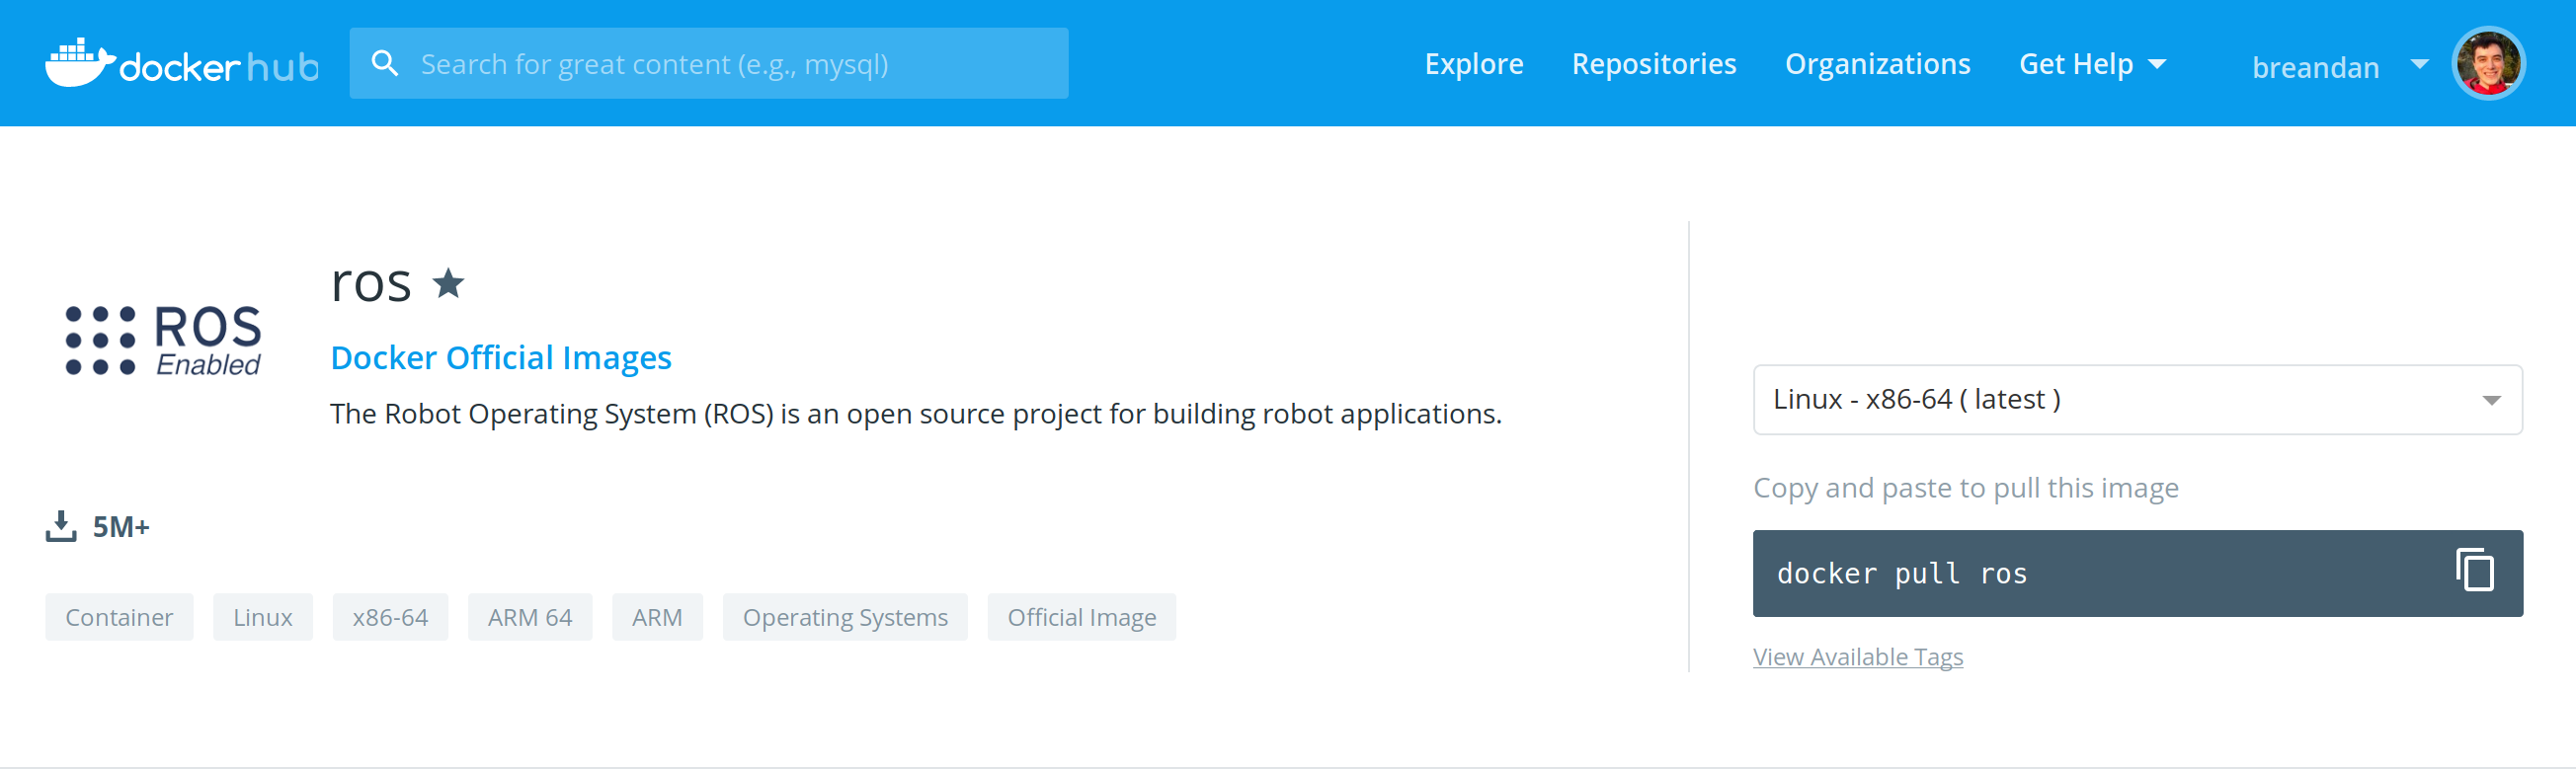
\includegraphics[width=\textwidth]{../figures/ros_docker_images.png}
\end{centering}

\subsection{\href{https://blog.hypriot.com/}{Hypriot}}\label{subsec:hypriot}

Hypriot, a base OS for RPi and other ARM devices, includes support for Docker straight out of the box. Hypriot is a lightweight Raspbian-based Linux distribution which \href{https://github.com/hypriot/image-builder-rpi}{builds} from the latest Raspberry Pi kernels and Raspbian releases.

\subsection{\href{https://www.piwheels.org/}{PiWheels}}

Not all Python packages (especially if they wrap a native library) can be run on all platforms. One might be tempted to build some package from its sources (and in rare cases, they might need to do so). But there is a good chance the package has already been compiled for Raspberry Pi on PiWheels. By using the following command (either in a \inline{Dockerfile} or via the CLI), various Python packages may be installed, e.g. \inline{opencv-python}:
%
\begin{rpilisting}
~$ pip install opencv-python --index-url https://www.piwheels.org/simple
\end{rpilisting}

\subsection{\href{https://hub.docker.com/}{Docker Hub}}\label{subsec:docker_hub}

Docker Hub is the central repository for Docker Images. Unless a separate registry has been configured, whenever users pull a Docker image tag, it will first query the Docker Hub for a matching image. The Docker Hub can be used to upload Docker images, and configure automated builds from GitHub (with a two hour build timeout). Docker Hub does not support layer caching of any kind, so the build will always take a fixed amount of time.\vspace{10pt}
%
\begin{centering}
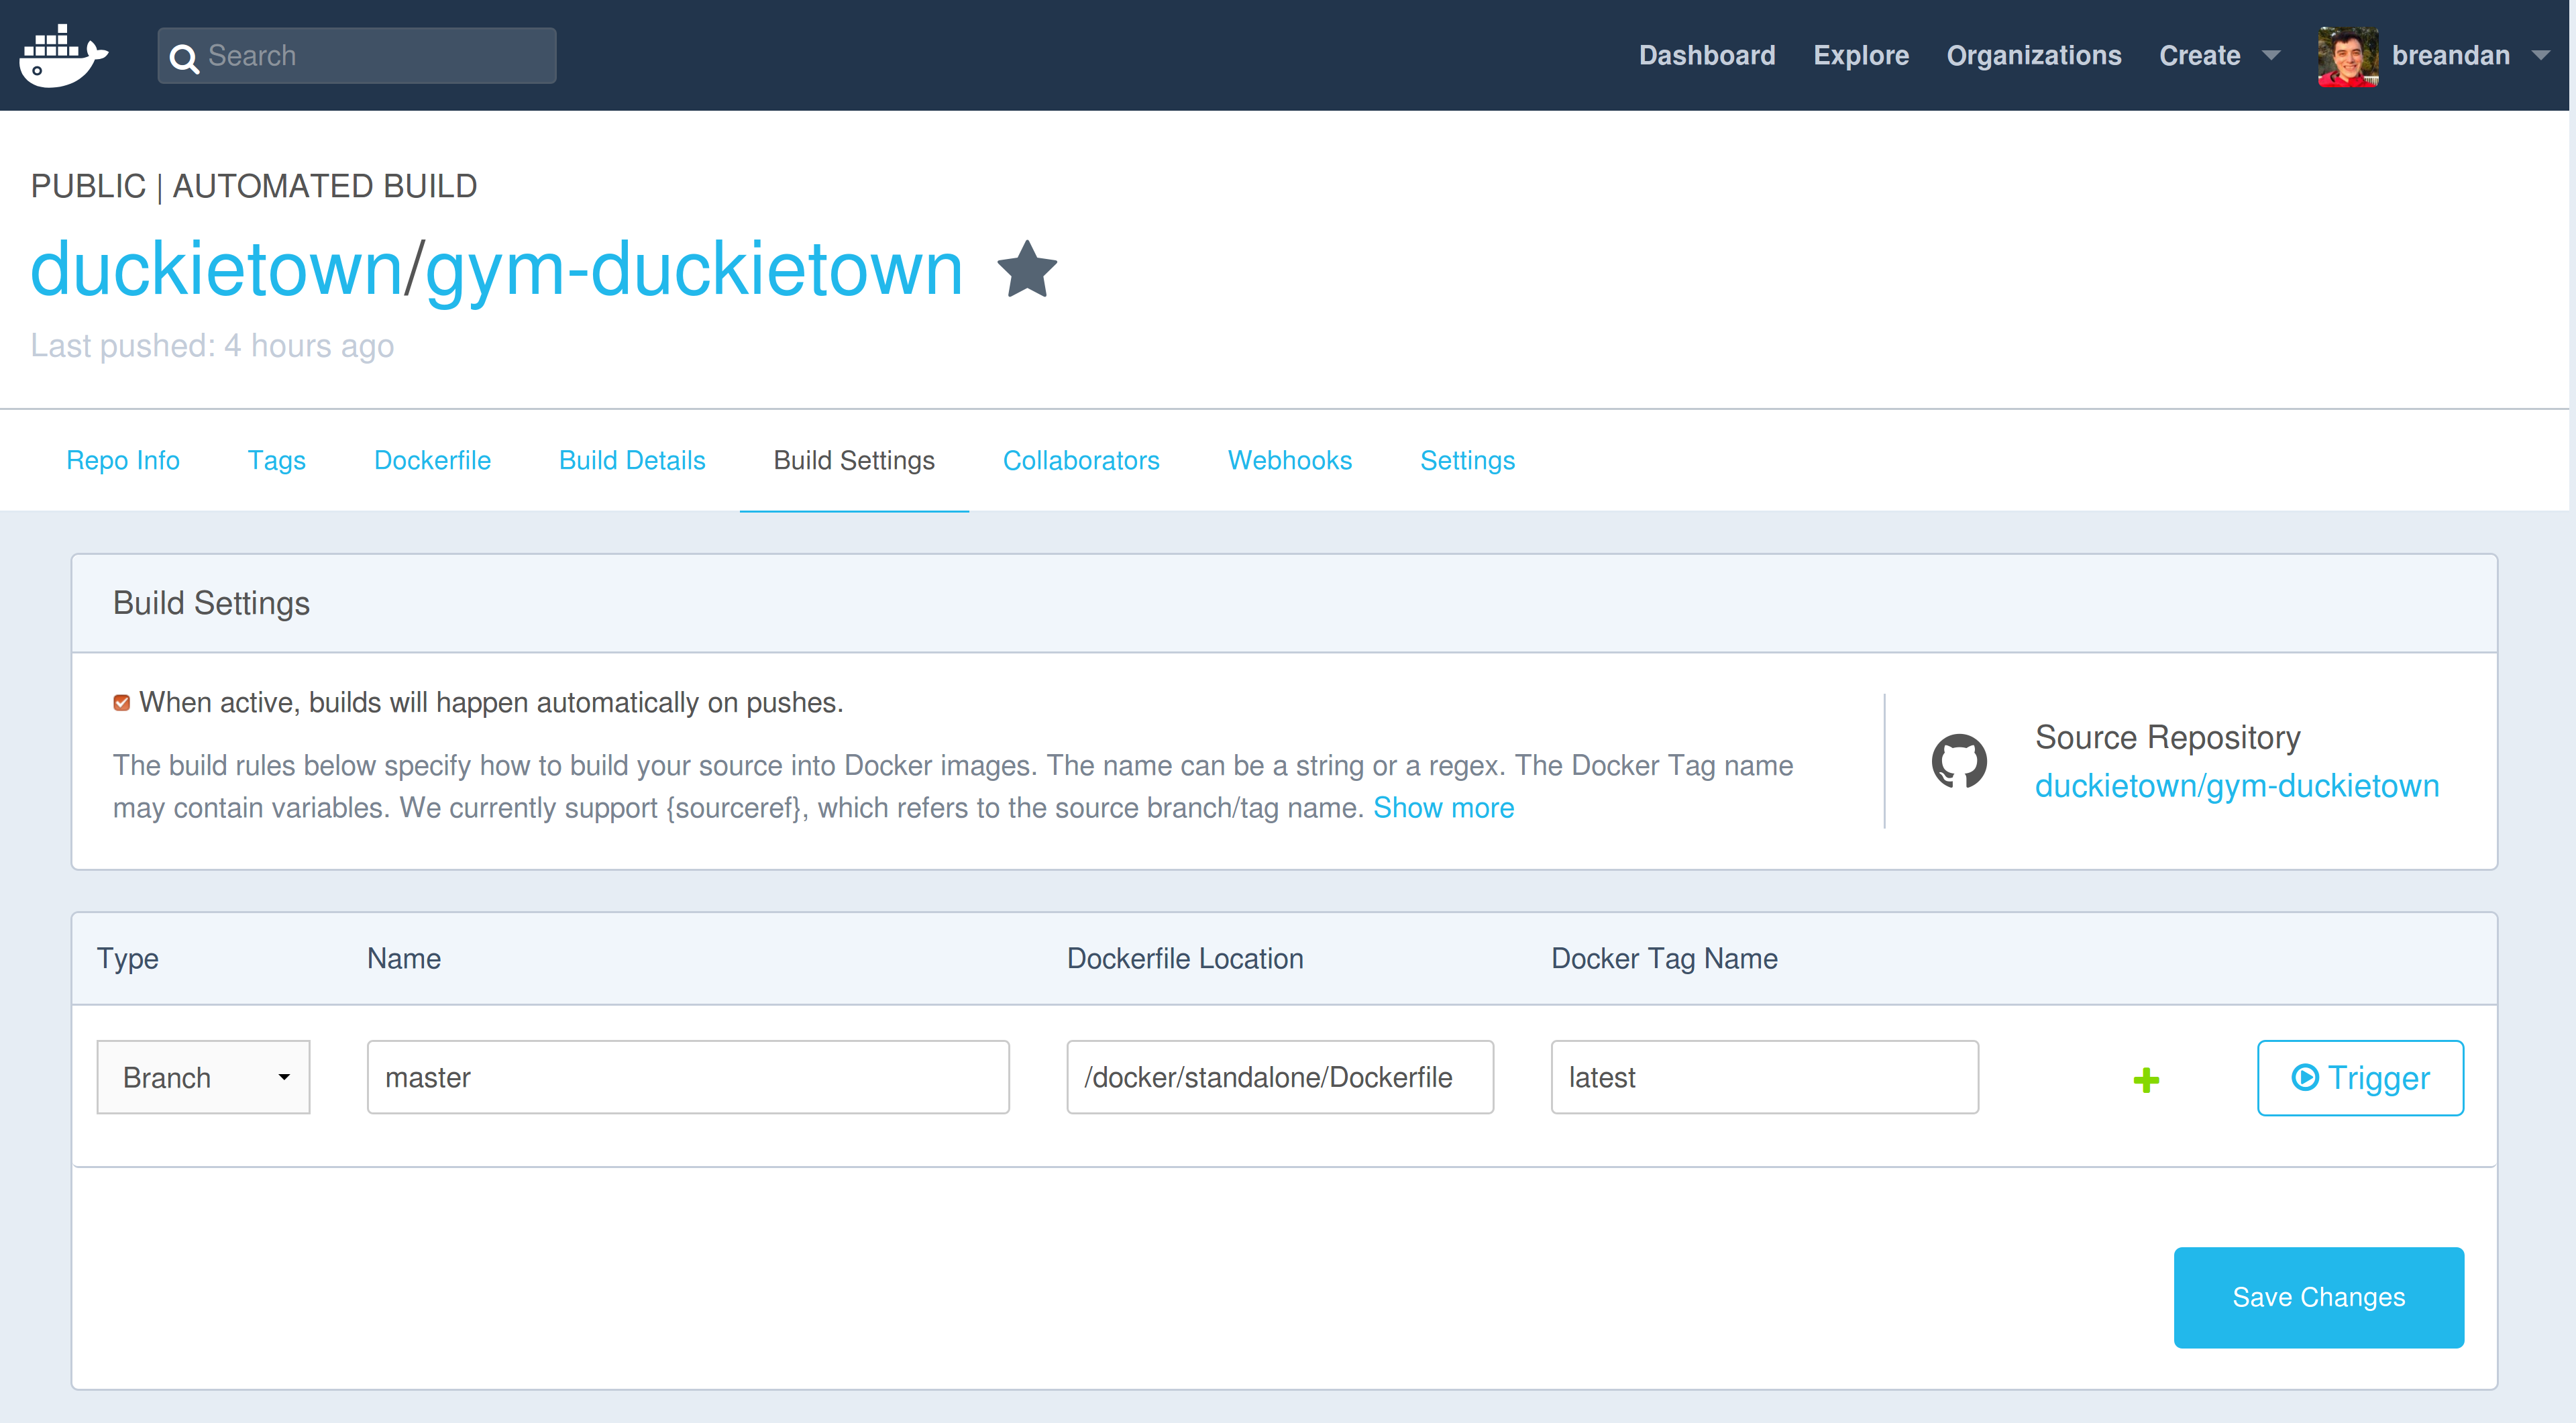
\includegraphics[width=\textwidth]{../figures/docker_hub_autobuild.png}
\end{centering}
%
Docker Hub auto-builds support linking a \inline{Dockerfile} in a GitHub repository, and whenever that \inline{Dockerfile} changes, the Docker image will be updated.

The Docker Hub also has features for configuring repository links and build triggers. These will automatically rebuild downstream Docker images whenever some event occurs.\vspace{10pt}
%
\begin{centering}
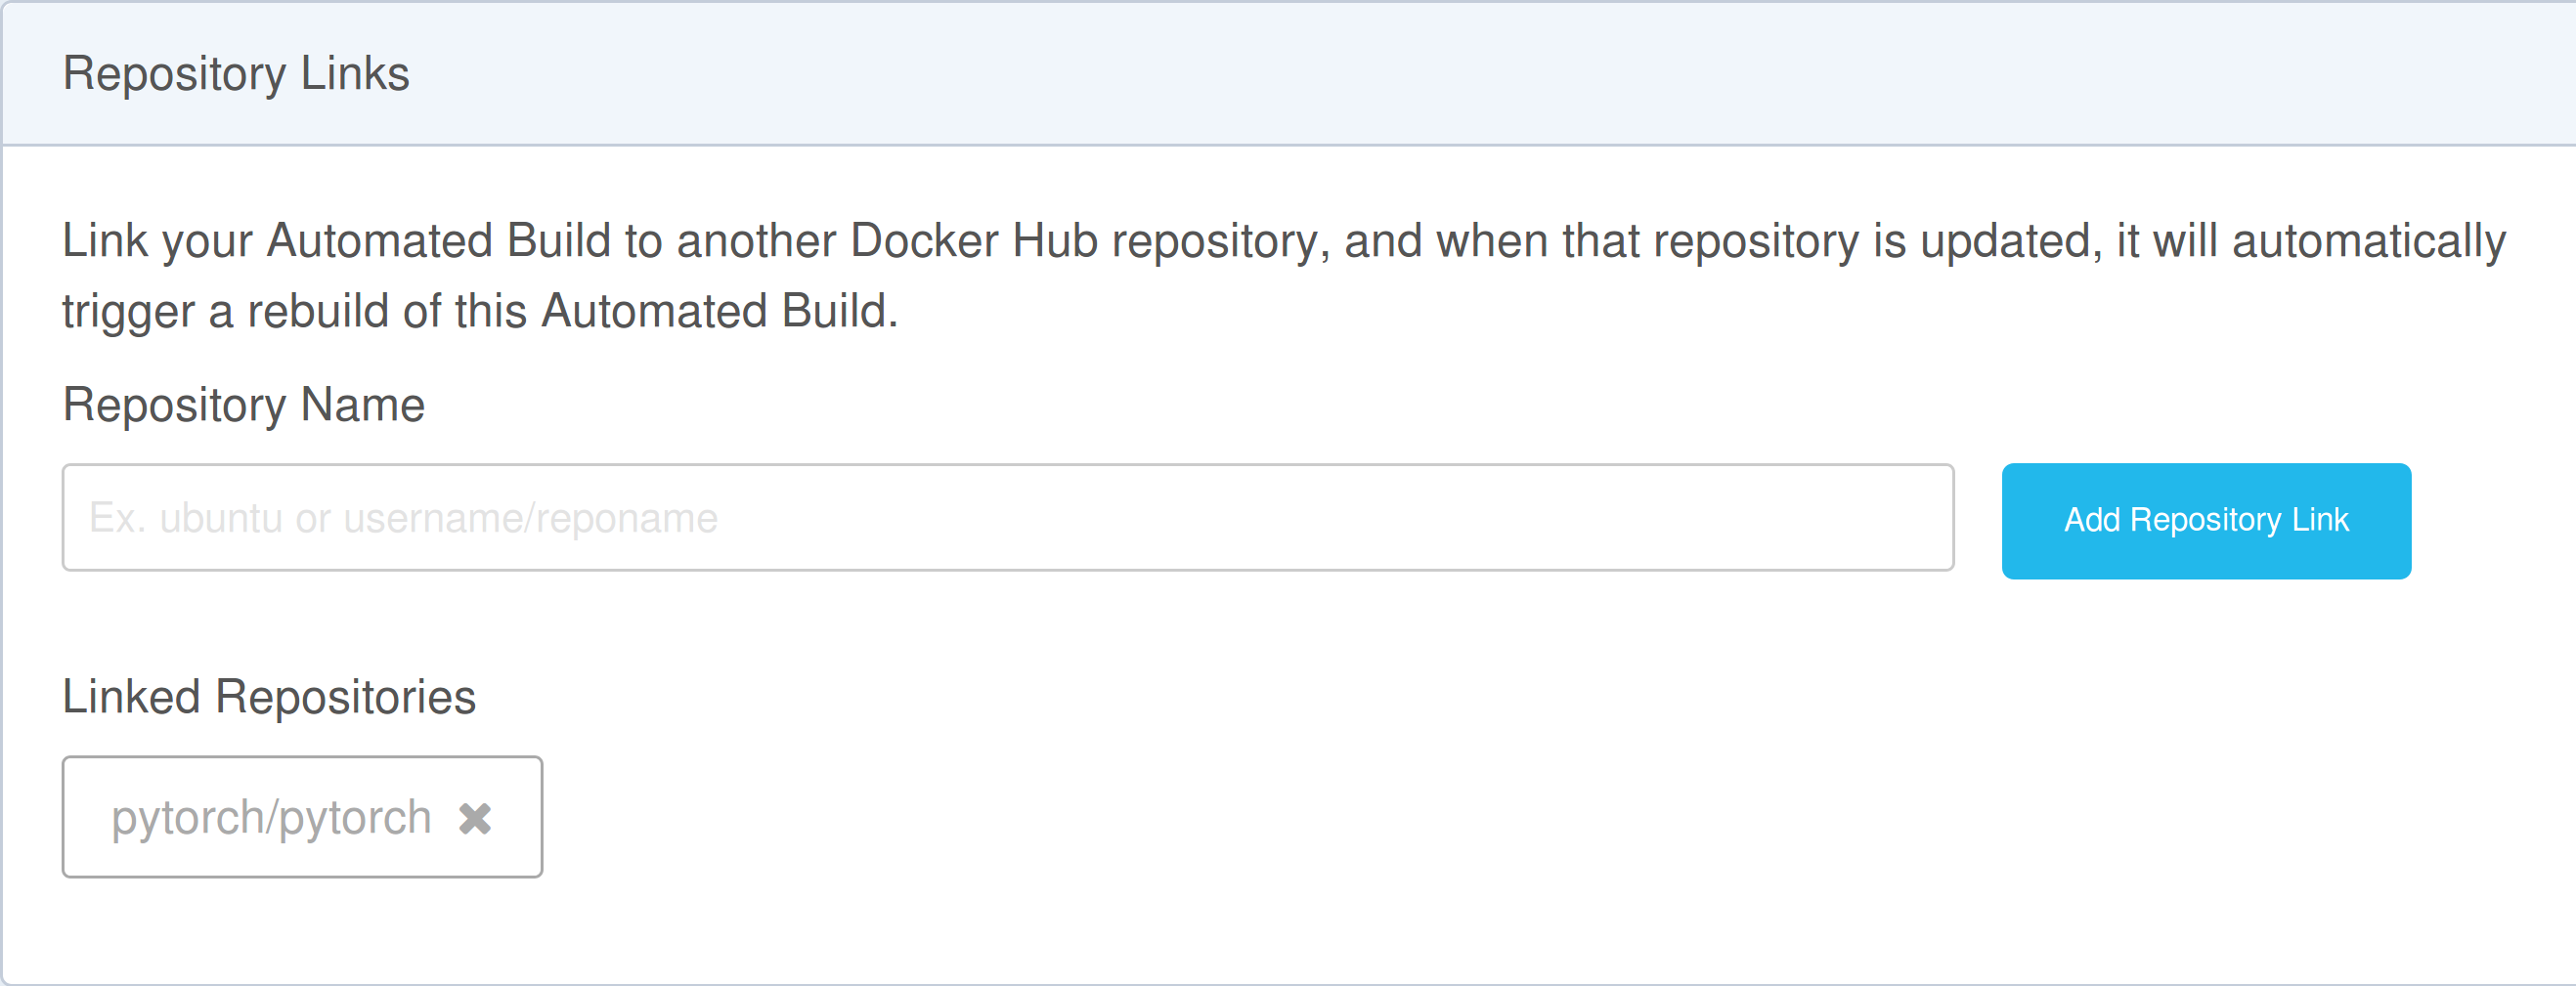
\includegraphics[width=\textwidth]{../figures/docker_hub_repo_links.png}
\end{centering}
%
Repository links allow support chaining builds together across Docker Hub repositories. Whenever a linked repository is updated, the dependent image will be rebuilt.

\subsection{\href{https://cloud.docker.com/}{Docker Cloud}}

Docker Cloud is a Docker registry which is fully integrated with the Docker Hub. Builds are automatically published from Docker Cloud to Docker Hub. Notifications for email and Slack, as well as longer build timeouts (up to 4-hours) are supported. Docker Cloud also supports more advanced build options than Docker Hub, such as a configurable build context and cache settings.\\

\begin{centering}
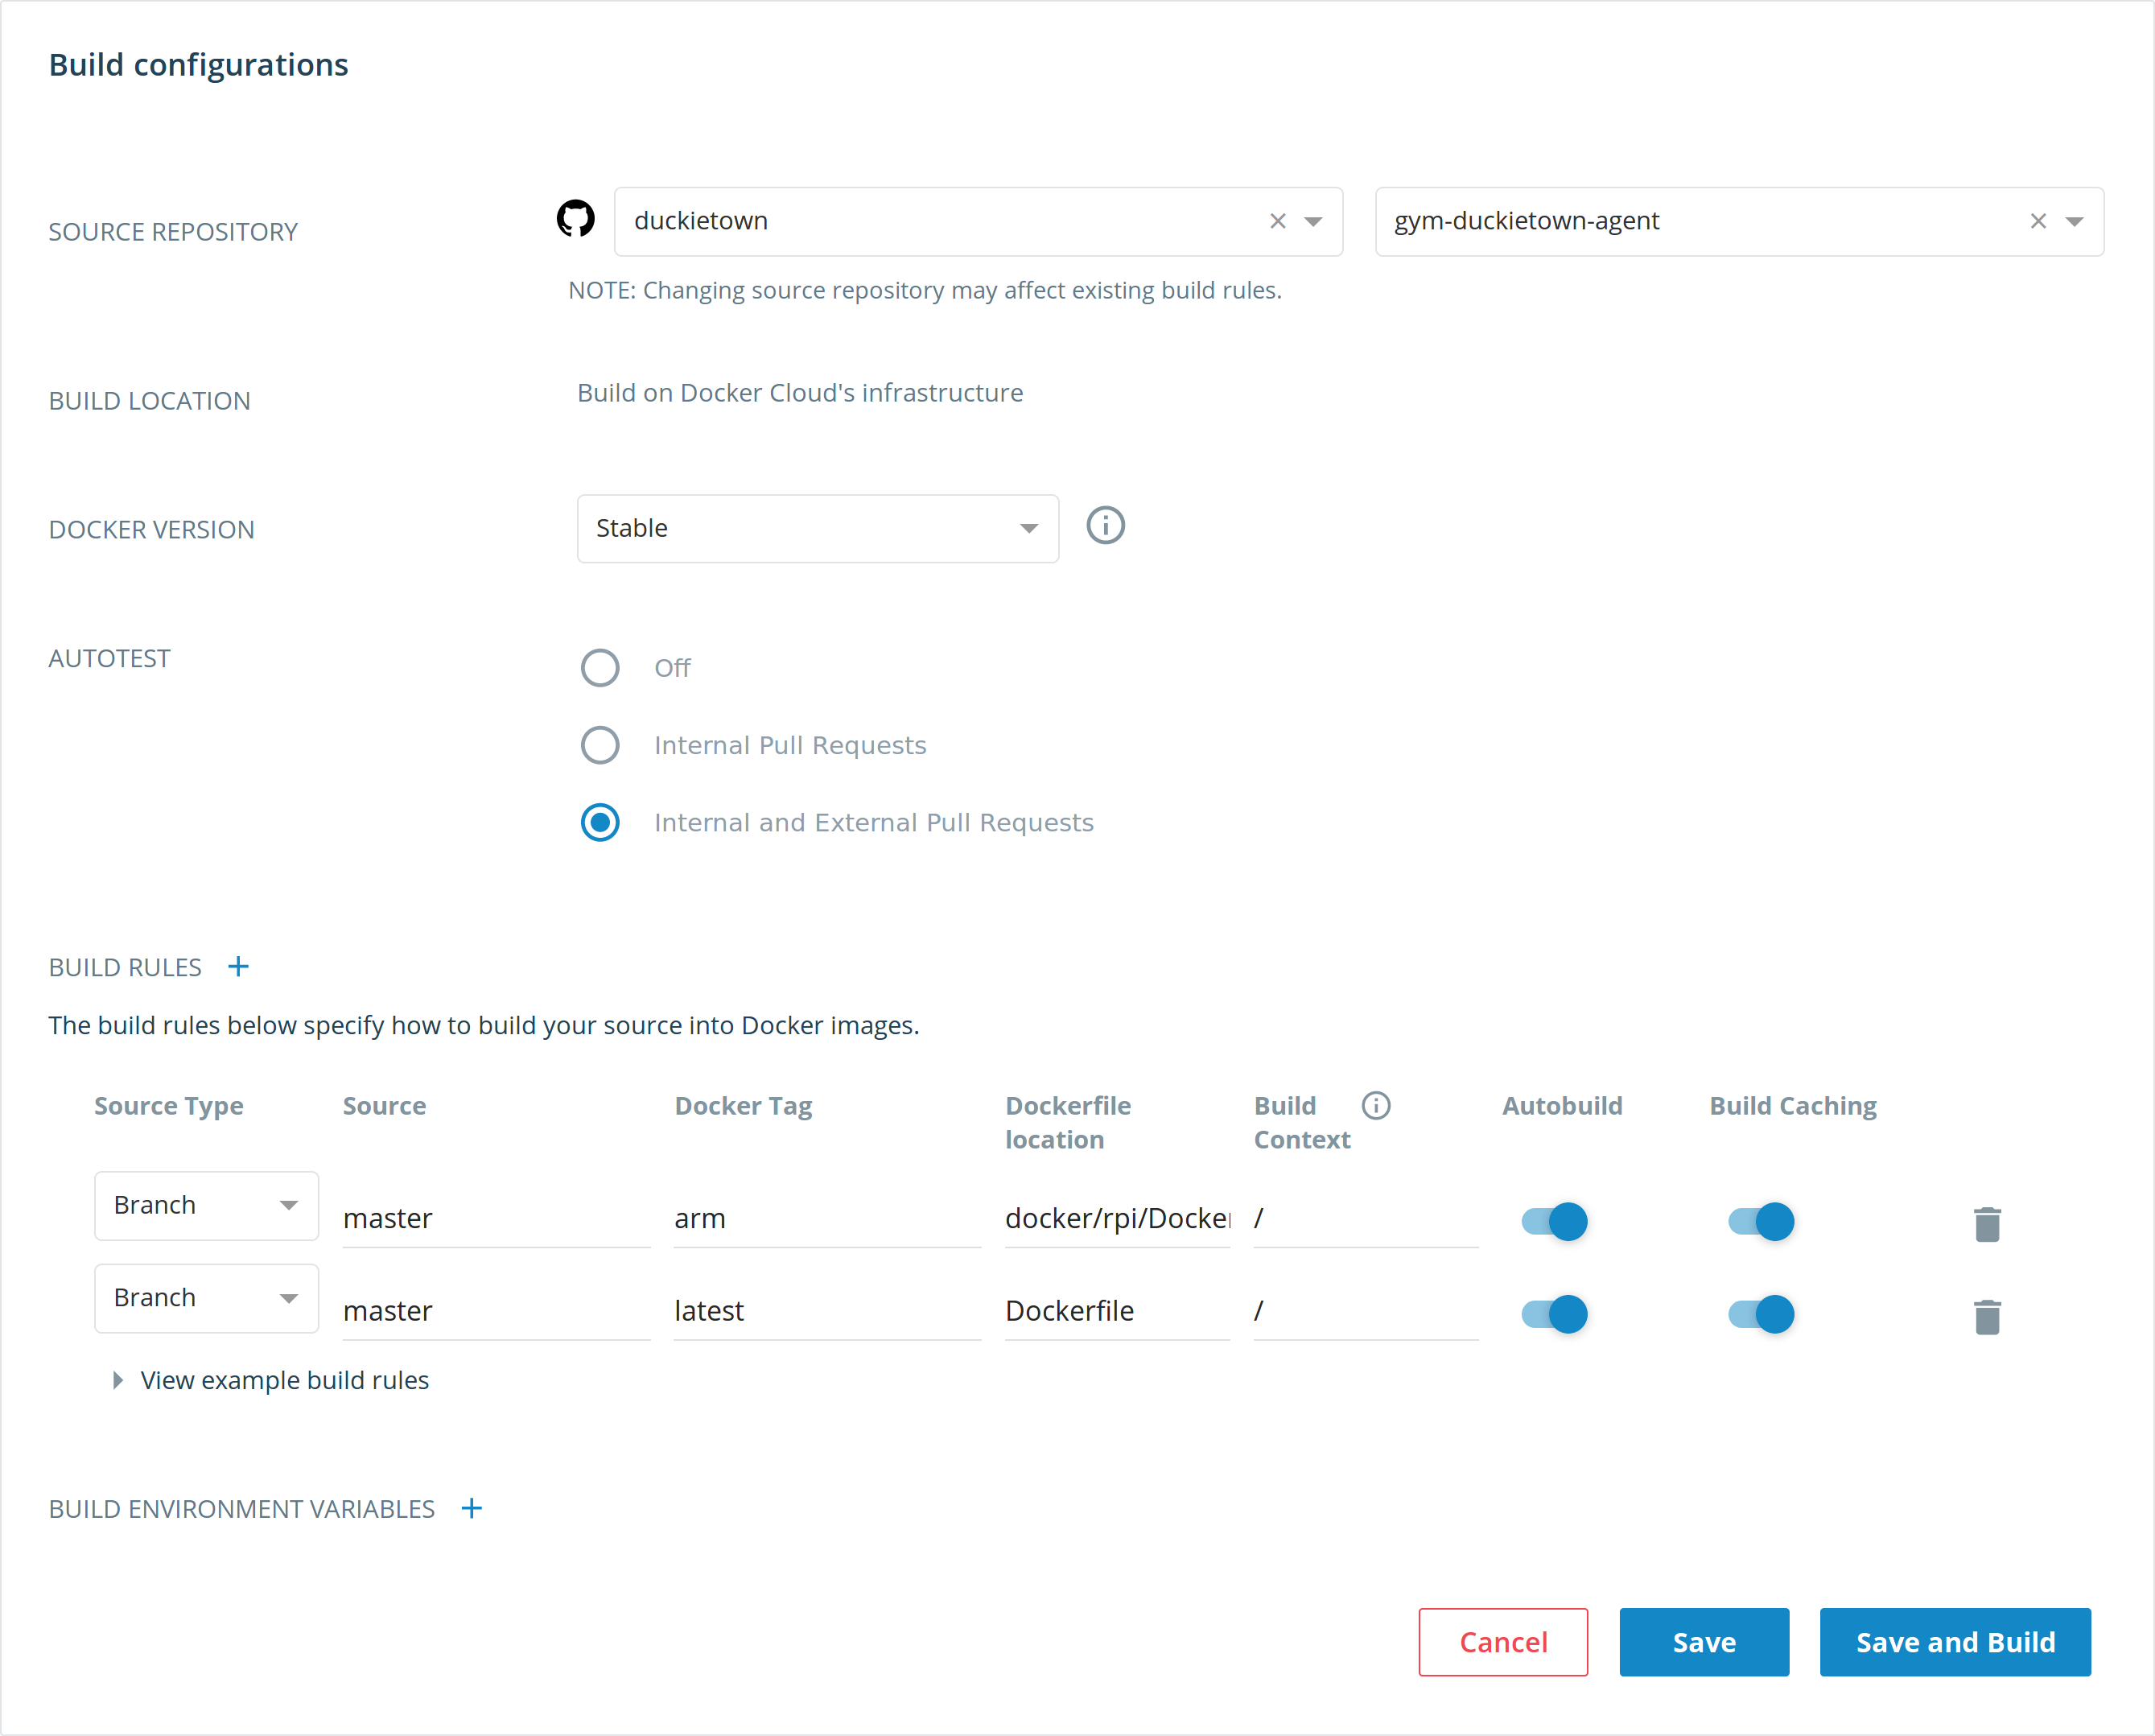
\includegraphics[width=\textwidth]{../figures/docker_cloud.png}
\end{centering}

\end{document}
